% Customizable fields and text areas start with % >> below.
% Lines starting with the comment character (%) are normally removed before release outside the collaboration, but not those comments ending lines

% svn info. These are modified by svn at checkout time.
% The last version of these macros found before the maketitle will be the one on the front page,
% so only the main file is tracked.
% Do not edit by hand!
\Rcs$Revision: 275627 $
\RCS$HeadURL: svn+ssh://svn.cern.ch/reps/tdr2/notes/AN-14-027/trunk/AN-14-027.tex $
\RCS$Id: AN-14-027.tex 275627 2015-01-31 14:43:15Z yxin $
%%%%%%%%%%%%% local definitions %%%%%%%%%%%%%%%%%%%%%
% This allows for switching between one column and two column (cms@external) layouts
% The widths should  be modified for your particular figures. You'll need additional copies if you have more than one standard figure size.
\newlength\cmsFigWidth
\ifthenelse{\boolean{cms@external}}{\setlength\cmsFigWidth{0.85\columnwidth}}{\setlength\cmsFigWidth{0.4\textwidth}}
\ifthenelse{\boolean{cms@external}}{\providecommand{\cmsLeft}{top}}{\providecommand{\cmsLeft}{left}}
\ifthenelse{\boolean{cms@external}}{\providecommand{\cmsRight}{bottom}}{\providecommand{\cmsRight}{right}}
%
%--- Our own macros:
\newcommand\qqbar{{\rm q\bar{q}}}
\newcommand\Hbb{\PH\to\bbbar}
\newcommand\Hww{\PH\to\PW\PW^*\to4{\rm q}}
\newcommand\Hzz{\PH\to\cPZ\cPZ^*\to4{\rm q}}
\newcommand\Zqq{\cPZ\to\qqbar}
%\newcommand\Vqq{V\to\qqbar}
\newcommand\HbbZqq{$\Hbb,\Zqq$}
\newcommand\HbbVqq{$\Hbb,\Vqq$}
\newcommand\HwwZqq{$\Hww,\Zqq$}
\newcommand\HwwVqq{$\Hww,\Vqq$}
\newcommand\Vqq{\PW/\cPZ\to\cPaq \Pq'}


%
%%%%%%%%%%%%%%%  Title page %%%%%%%%%%%%%%%%%%%%%%%%
\cmsNoteHeader{AN-14-027} % This is over-written in the CMS environment: useful as preprint no. for export versions
% >> Title: please make sure that the non-TeX equivalent is in PDFTitle below
%\title{Search for heavy resonances in the W/Z-tagged dijet mass spectrum in pp collisions at 8 TeV}
%\title{Search for heavy resonances in H/W/Z-tagged dijet mass spectrum in pp collisions at 8 TeV}
\title{Search for massive WH and ZH resonances in dijet systems containing jets tagged
as W or Z or H boson decays in pp collisions at $\sqrt{s}= 8\TeV$}

% >> Authors
%Author is always "The CMS Collaboration" for PAS and papers, so author, etc, below will be ignored in those cases
%For multiple affiliations, create an address entry for the combination
%To mark authors as primary, use the \author* form
\address[cern]{CERN}
\address[uzh]{University of Zurich}
\address[jhu]{Johns Hopkins University}
\address[lyon]{Universite Claude Bernard-Lyon I}
\address[SPRACE]{SPRACE-UNESP}

\author[jhu]{Yongjie Xin}
\author[uzh]{Andreas Hinzmann}
\author[jhu]{Petar Maksimovi\'c}
\author[lyon]{Maxime Gouzevich}
\author[lyon]{Alexandra Carvalho}
\author[cern]{Maurizio Pierini}
\author[SPRACE]{Thiago R.F.P. Tomei}

\newcommand{\re}{\ensuremath{\cmsSymbolFace{e}}}
\newcommand{\scalefactorHP}{ \ensuremath{0.86 \pm 0.07}\xspace}
\newcommand{\scalefactorLP}{ \ensuremath{1.39 \pm 0.75}\xspace}
\newcommand{\scalefactorHPu}{ \ensuremath{7.5\%}\xspace}
\newcommand{\scalefactorLPu}{ \ensuremath{54\%}\xspace}
\newcommand{\GRS}{\ensuremath{G_\mathrm{RS}}\xspace}
\newcommand{\GBulk}{\ensuremath{G_\mathrm{Bulk}}\xspace}
\newcommand{\MPl}{\ensuremath{\overline{M}_\text{Pl}}\xspace}


\newcommand{\rsgwwintervalone}{$[1.0 \TeVcc, 1.04 \TeVcc]$}
\newcommand{\rsgwwintervaltwo}{$[1.16 \TeVcc, 1.22 \TeVcc]$}
\newcommand{\rsgwwexplimit}{1.13\TeV}

\newcommand{\pdf}{\ensuremath{\mathrm{pdf}}}
\newcommand{\ta}{\mbox{$\tau$}}
\renewcommand{\ttbar}{\ensuremath{\mathrm{t}\bar{\mathrm{t}}}~}
\newcommand{\mtt}{\ensuremath{m_{\mathrm{t}\bar{\mathrm{t}}}}~}
%\newcommand{\zp}{\ensuremath{{\mathrm{Z^{\prime}}}}}
\newcommand{\wboson}{\ensuremath{{\mathrm{W}}}}
\newcommand{\zboson}{\ensuremath{{\mathrm{Z}}}}
\newcommand{\mzp}{\ensuremath{m_{\mathrm{Z^{\prime}}}}}
\newcommand{\qq}{\ensuremath{\mathrm{q}\bar{\mathrm{q}}}}
%\newcommand{\qq}{$\mathrm{q}\bar{\mathrm{q}}$~}
\newcommand{\invpb}{pb$^{-1}$~}
\newcommand{\intlumi}{19.7~fb$^{-1}$}
\newcommand{\wmasssemilepdata}{ \ensuremath{m_\wboson^{\mathrm{DATA}} = 82.893 \pm 0.285 \; \GeVcc}~} 
\newcommand{\wmasssemilepmc}{ \ensuremath{m_\wboson^{\mathrm{MC}} = 82.747 \pm 0.178 \; \GeVcc}~} 
\newcommand{\topmasssemilepdata}{ \ensuremath{m_{\mathrm{t}}^{\mathrm{DATA}} = 177.1 \pm 2.0 \; \GeVcc}~} 
\newcommand{\topmasssemilepmc}{ \ensuremath{m_{\mathrm{t}}^{\mathrm{MC}} = 171.5 \pm 0.7 \; \GeVcc}~} 
\newcommand{\subjetjes}{\ensuremath{1.002 \pm 0.004}~}
%\newcommand{\mcuteffsemilepdata}{ \ensuremath{\epsilon_{m_\wboson}^{\mathrm{DATA}} = 0.525 \pm 0.007}~} 
%\newcommand{\mcuteffsemilepmc}{ \ensuremath{\epsilon_{m_\wboson}^{\mathrm{MC}} =  0.558 \pm 0.006}~} 
%\newcommand{\mucuteffsemilepdata}{ \ensuremath{\epsilon_\mu^{\mathrm{DATA}} = 0.210 \pm 0.002}~} 
%\newcommand{\mucuteffsemilepmc}{ \ensuremath{\epsilon_\mu^{\mathrm{MC}} =  0.222 \pm 0.002}~} 
\newcommand{\PYTHIAEIGHT} {{\textsc{pythia8}}\xspace}
\newcommand{\qWlimit}{2.38 TeV}
\newcommand{\qZlimit}{2.15 TeV}
\newcommand{\qWexplimit}{2.43 TeV}
\newcommand{\qZexplimit}{2.07 TeV}



% >> Date
% The date is in yyyy/mm/dd format. Today has been
% redefined to match, but if the date needs to be fixed, please write it in this fashion.
% For papers and PAS, \today is taken as the date the head file (this one) was last modified according to svn: see the RCS Id string above.
% For the final version it is best to "touch" the head file to make sure it has the latest date.
\date{\today}

% >> Abstract
% Abstract processing:
% 1. **DO NOT use \include or \input** to include the abstract: our abstract extractor will not search through other files than this one.
% 2. **DO NOT use %**                  to comment out sections of the abstract: the extractor will still grab those lines (and they won't be comments any longer!).
% 3. **DO NOT use tex macros**         in the abstract: External TeX parsers used on the abstract don't understand them.
\abstract{
%  This is a search of massive resonannce decaying into Higgs and a vector boson,
%   where each boson decays into hadronic final states.  This
%  search has been performed on the proton-proton collision data collected
%  with the CMS experiment at the LHC in 2012 at a center-of-mass
%  energy of 8 TeV and corresponding to an integrated luminosity of
%  19.7/fb.
%  The boosted vector bosons are identified using novel jet
%  substructure identification techniques. The Higgs bosons are identified by different 
%  techniques with respect to different decay channels. Higgs decays to b quarks are identified by 
%  b-tagging on the two subjets. While Higgs to WW to qqqq quarks are identified by N-subjettiness.  
  A search for massive resonances decaying into a
   Higgs boson (125 GeV) and a W or a Z boson is reported.
  The analysis is
  performed on an inclusive sample of multijet events corresponding to
  an integrated luminosity of 19.7\fbinv,  collected in
  proton-proton collisions at a centre-of-mass energy of 8\TeV with
  the CMS detector at the LHC. %The Higgs bosons are identified by different 
  %techniques with respect to different decay modes. 
  Jets from Higgs decaying into
  $b$-quark pairs are identified by subjets/jets $b$-tagging.
  The search also uses jet-substructure
  identification techniques that provide sensitivity to the presence of
  highly boosted Higgs bosons decaying into hadronic W pairs and vector bosons
  decaying into a pair of quarks.
%  Limits are setting on W' and Z' bosons, decaying into one Higgs boson and 
%  one vector boson. We exclude Z' resonances up to mass of 1.3TeV. 
  Exclusion limits are set at a confidence level of 95\% on the production of %: 
  Z' decaying into HZ for masses in [1.0, 1.1] TeV and [1.3, 1.5] TeV,  and
  W' decaying into HW for masses in [1.0, 1.6] TeV.

} 

% >> PDF Metadata
% Do not comment out the following hypersetup lines (metadata). They will disappear in NODRAFT mode and are needed by CDS.
% Also: make sure that the values of the metadata items are sensible and are in plain text:
% (1) no TeX! -- for \sqrt{s} use sqrt(s) -- this will show with extra quote marks in the draft version but is okay).
% (2) no %.
% (3) No curly braces {}.
\hypersetup{%
  pdfauthor={Andreas Hinzmann, Petar Maksimovic, Yongjie Xin},%
  pdftitle={Search for heavy resonances in the HZ-tagged dijet mass
    spectrum in pp collisions at 8 TeV},%
pdfsubject={CMS},%
pdfkeywords={CMS, physics, dijet, jet substructure, resonances}}

\maketitle %maketitle comes after all the front information has been supplied
\tableofcontents
% >> Text
%%%%%%%%%%%%%%%%%%%%%%%%%%%%%%%%  Begin text %%%%%%%%%%%%%%%%%%%%%%%%%%%%%
%% **DO NOT REMOVE THE BIBLIOGRAPHY** which is located before the appendix.
%% You can take the text between here and the bibiliography as an example which you should replace with the actual text of your document.
%% If you include other TeX files, be sure to use "\input{filename}" rather than "\input filename".
%% The latter works for you, but our parser looks for the braces and will break when uploading the document.
%%%%%%%%%%%%%%%
%\section*{To-do list}

This is what still needs to be added to the note:

\begin{enumerate}


%\item High priority: the data/MC scale factor for the
%  $\tau_{42}$ cut (and its uncertainty) in $\Hww$ channel.
%  Status: the HERWIG++ samples are in hand, and are being processed.

%\item High priority: figure out how to obtain the theoretical curves
%  for the limit plots.  In fact, these are simplified models and we
%  may need to figure out how to quote the limits.

\item Medium priority: add the description of the simplified models
  into the introduction section.

\item Low priority: Document the study of the impact of changing the value of
  the $\tau_{42}$ cut as a function of the resonance mass.  We decided
  against using this so this is just for completeness.

%\item Low priority: Add to the Appendix the comparison betwen the limits while using
%  CSVL vs CSVM for the fat jet b tagging.

\end{enumerate}




\chapter{Search for X $\to$ WH or ZH at LHC at $\sqrt{s} = 8$~TeV }
\label{chap:chapter4}
\section{Introduction}
\label{sec:introduction}


Several theories of physics beyond the standard model (SM) predict the
existence of vector resonances with
masses above 1\TeVcc that decay into
a W or Z vector boson (V)
 and a SM-like Higgs boson (H).
Here we present a search for 
the production of such resonances
 in proton-proton (pp) collisions at a
centre-of-mass energy of $\sqrt{s}=8$\TeVcc.  The data sample,
corresponding to an integrated luminosity of 19.7\fbinv, was collected
with the CMS detector at the CERN LHC.


%The following models of ${\rm \PWpr\to HW}$ and ${\rm Z'\to HZ}$ resonances are considered in this analysis.

The composite Higgs~\cite{Composite0,Composite1,Composite2} and little Higgs models~\cite{Han:2003wu}
address the issue of the hierarchy problem and predict many new particles,
%provide a direct solution to the hierarchy problem and 
including additional gauge bosons, e.g. heavy spin-1 $\PWpr$ or ${\rm Z'}$ bosons.
These models can be generalized in the Heavy Vector Triplet (HVT)~\cite{Pappadopulo:2014qza}
framework.
Of particular interest for this search is the HVT scenario B model, where
the branching fraction $\mathcal{B}({\rm W' \to WH})$ and $\mathcal{B}({\rm Z' \to ZH}) $ dominate over the corresponding 
branching fractions to fermions, and are comparable to $\mathcal{B}({\rm W' \to WZ})$ 
and $\mathcal{B}({\rm Z' \to WW})$. 
In this scenario, experimental constraints from searches for boson decay 
channels are more stringent than those from fermion decay channels. 
Several searches~\cite{Khachatryan:2014xja,
Aad:2014pha,Aad:2014xka,ATLASWWPAPER,EXO-12-024} 
for ${\rm W^\prime \rightarrow WZ}$ 
based upon the Extended Gauge Boson (EGB) reference 
model~\cite{egm} have excluded resonance 
masses below 1.7\TeVcc. Unlike the HVT scenario B model, 
the EGB model has enhanced fermionic couplings 
and the mass limit is not directly 
comparable to this work. Model independent limits on 
the cross section for the resonant 
production $\ell\nu+\mathrm{jets}$~\cite{EXO-13-009} can 
be used to extract resonance mass 
limits on the the processes ${\rm W^\prime\rightarrow WZ}$ 
and ${\rm Z^\prime \rightarrow WW}$ of 
1.7 TeV and 1.1 TeV, respectively.
A search for ${\rm Z^\prime \rightarrow ZH \rightarrow q\bar{q}}\tau\tau$
was reported in Ref.~\cite{cms-HZ-tautaujet} and
interpreted in the context of HVT scenario model B; however, 
no resonance mass limit could be set with the sensitivity achieved.
Finally, a recent search~\cite{Aad:2015yza} combining leptonic
decays of W and Z bosons, and two b-tagged jets forming a ${\rm \Hbb}$ candidate
excluded HVT model A with coupling constant $g_V = 1$ for heavy vector
boson masses below $m_{V'^0} < 1360~\GeV$ and $m_{V'^\pm} < 1470~\GeV$.

The signal of interest is a narrow heavy vector resonance ${\rm V'}$ decaying into
VH, where the V decays to a pair of quarks and the H decays either to
a pair of b quarks, or to a pair of W bosons, which further decay into
quarks.
The H in the HVT framework does not have properties that are identical 
to those of a SM Higgs boson. We make the assumption that the state 
observed by the LHC Collaborations~\cite{higgsdiscoveryAtlas,Chatrchyan:2012ufa} 
is the same as the one described by the HVT framework and 
that, in accord with present 
measurements~\cite{Khachatryan:2014kcaCMSHiggs1,Khachatryan:2014jbaCMSHiggs2,AtlasHiggs1}, 
its properties are similar to those of a SM Higgs boson.
  
In the decay of massive ${\rm V'}$ bosons 
produced in the pp collisions at the LHC, 
the momenta of the daughter V and H are large enough (${>} 200\GeV$) 
that their hadronic decay products 
are reconstructed as single jets~\cite{Gouzevitch:2013qca}. 
Because this results in a dijet topology, 
traditional analysis techniques relying on resolved jets are 
no longer applicable. The signal is characterized by a peak 
in the dijet invariant mass ($m_\mathrm{jj}$) distribution 
over a continuous background from mainly QCD multijet 
events. The sensitivity to b-quark jets 
from H decays is enhanced through 
subjet or jet b tagging~\cite{BTV-13-001}. 
Jets from ${\rm \Vqq}$, ${\rm \Hbb}$, and ${\rm \Hww}$ 
(virtual W denoted with an asterisk)
decays are identified with jet 
substructure techniques~\cite{topwtag_pas,JME-13-006}.


This is the first search for heavy resonances 
decaying via VH into all-jet final states 
and it incorporates the first application of jet substructure 
techniques to identify ${\rm \Hww}$ at a high Lorentz boost.


This analysis proceeds via the following steps:
\begin{enumerate}
\item The search is performed in the dijet sample, using the same
      preselection as the standard search for resonances decaying to 
      dijets~\cite{cmsdijet, cmsdijet8TeV}.

\item We identify events with one W/Z boson jet: a candidate
  jet originating from merged decaying products of W/Z:  
  \begin{itemize}
  \item we require a pruned jet mass cut, and
  \item an N-subjettiness cut preferring two-prong decays
  \end{itemize}
  (This is identical to Chapter~\ref{chap:chapter3}.)

\item We identify events with a highly boosted Higgs boson:
  \begin{itemize}
  \item we require a pruned jet mass cut, and
  \item two b tagged subjets, or 
  \item (when there are no two b tagged subjets) a N-subjettiness cut
    preferring four subjets
  \end{itemize}
  (The ${\rm \Hbb}$ tagging is synchronized with our sister analysis, the Radion
  search to the HH final state~\cite{HH4b}.)

\item After the full event selection, a potential signal would be
  characterized as a peak in the dijet invariant mass, on top of a
  falling background distribution.  

\item We model the background distribution with a smoothly falling 
  analytical function.  (The functional form is identical
  to the one used in Chapter~\ref{chap:chapter3}.)

\item We form the joint likelihood of several dijet distributions
  of V tagged and H tagged jets.  We include both two types of
  Higgs tags, and also low-purity Higgs and V taggers.  The background
  estimate procedure is the same in all channels -- analytical
  parametrization -- but is performed separately for each channel.

\item Finally, we set the limits on the various simplified models
  for resonances decaying to HV final states.

\end{enumerate}

%\newpage
\section{CMS detector}
\label{sec:cms_detector}


The CMS detector~\cite{:2008zzk}
is a general-purpose device, however it has
many features particularly suited for reconstruction of 
energetic jets, specifically, the finely segmented electromagnetic
and hadronic calorimeters, as well as the charged particle tracking.
The charged particles are reconstructed by the inner tracker,
immersed in a $3.8$~T axial magnetic field; the inner tracker consists
of three cylindrical layers and two endcap disks of pixel sensors, and ten
barrel layers and twelve endcap disks of silicon strips.  This
arrangement results
in a full azimuthal coverage within $|\eta| < 2.5$, where $\eta$
is the pseudorapidity defined as $\eta = -\ln\tan(\theta/2)$.
CMS uses a polar coordinate system, with the 
$z$ axis coinciding with the axis of symmetry of the CMS detector,
and oriented in the counterclockwise proton direction; $\theta$ 
is the polar angle defined with respect to the positive $z$ axis.
%The pseudorapidity is an approximation for the full rapidity $y$, and
%the approximation is exact for massless particles.
%Since many of the
%particles we use are not massless, we use the full rapidity $y$ which
%is defined as $y = \frac{1}{2} \frac {E + p_{z}/c}{E - p_{z}/c}$.

A lead-tungstate crystal electromagnetic calorimeter (ECAL) and 
a brass-scintillator hadronic calorimeter (HCAL) surround the tracking
volume and allow photon, electron and jet reconstruction up to $|\eta|=3$.
The ECAL and HCAL cells are grouped into towers projecting radially 
outward from the interaction region.  In the central region ($|\eta|<1.74$)
the towers have dimensions $\Delta\eta = \Delta\phi = 0.087$; however,
at higher $\eta$, the $\Delta\eta$ and $\Delta\phi$ widths increase.  
ECAL and HCAL
cell energies above the noise suppression thresholds are combined within
each tower to define the calorimeter tower energy. The towers are further
combined into clusters, which are then identified as jets.  For an improved
jet reconstruction, the tracking and calorimeter information is combined 
in an algorithm called particle-flow~\cite{particleflow}, which is described
below.
%\clearpage

%\newpage
\section{Hbb HWW and other Channels}
\label{sec:contamination}

Hbb, Hww tagger will also pick up Higgs signals from other channels of Higgs decay. 
In Table~\ref{table:HbbHww}, branching ratio column is taken from standard model Higgs decays at 125GeV. 
For H(ww$\to$qqqq), the branching ratio of W hadronicly decay is already considered. 
Here we assume we have 100000 Standard Model Higgs, and the numbers in the table are showing the number of Higgs pass
the tagger for each channel, with branching ratio taken into account. 
For example, Hcc part, of 100000 SM Higgs,  in Hcc channel, at 1TeV Z' resonance, which is 0.5TeV Higgs, 
we will have 104.42 events pass the Hbb tagger and 102.41 pass the Hww tagger and we also have 82.33 events which fail the 
Hbb tagger but pass the Hww tagger.  

Considering this table, our analysis will move like this way. 
We will keep the Hbb tagger as it was. 
For the Hww channel, we will only select events that fail the Hbb tagger, but pass Hww tagger.
And the effects of this on the background is shown in Fig~\ref{fig:HbbRatio} 


\begin{table}[htbp]
\caption{}
\begin{tabular}{|l|r|r|r|r|}
\hline
1TeV & \multicolumn{1}{l|}{Braching Ratio} & \multicolumn{1}{l|}{Hbb tagger} & \multicolumn{1}{l|}{Pass Hww tagger} & \multicolumn{1}{l|}{Fail Hbb, pass Hww} \\ \hline
Hbb & 57.70 & 11871.78 & 1765.62 & 804.92 \\ \hline
Hww$\to$qqqq & 9.94 & 86.98 & 2416.41 & 2360.75 \\ \hline
Hcc & 3.00 & 104.42 & 102.41 & 82.33 \\ \hline
Htautau & 6.30 & 17.33 & 47.25 & 37.80 \\ \hline
Hgg & 10.00 & 14.99 & 344.83 & 314.84 \\ \hline
 & \multicolumn{1}{l|}{} & \multicolumn{1}{l|}{} & \multicolumn{1}{l|}{} & \multicolumn{1}{l|}{} \\ \hline
1.5TeV & \multicolumn{1}{l|}{Braching Ratio} & \multicolumn{1}{l|}{Hbb tagger} & \multicolumn{1}{l|}{Pass Hww tagger} & \multicolumn{1}{l|}{Fail Hbb, pass Hww} \\ \hline
Hbb & 57.70 & 11444.80 & 1849.29 & 755.87 \\ \hline
Hww$\to$qqqq & 9.94 & 228.62 & 2043.17 & 1916.43 \\ \hline
Hcc & 3.00 & 121.25 & 113.43 & 88.01 \\ \hline
Htautau & 6.30 & 12.60 & 67.10 & 57.02 \\ \hline
Hgg & 10.00 & 69.93 & 244.76 & 174.83 \\ \hline
 & \multicolumn{1}{l|}{} & \multicolumn{1}{l|}{} & \multicolumn{1}{l|}{} & \multicolumn{1}{l|}{} \\ \hline
2TeV & \multicolumn{1}{l|}{Braching Ratio} & \multicolumn{1}{l|}{Hbb tagger} & \multicolumn{1}{l|}{Pass Hww tagger} & \multicolumn{1}{l|}{Fail Hbb, pass Hww} \\ \hline
Hbb & 57.70 & 13816.27 & 1834.86 & 551.04 \\ \hline
Hww$\to$qqqq & 9.94 & 449.29 & 1655.51 & 1435.83 \\ \hline
Hcc & 3.00 & 228.57 & 133.33 & 99.05 \\ \hline
Htautau & 6.30 & 42.21 & 97.34 & 74.66 \\ \hline
Hgg & 10.00 & 157.62 & 315.24 & 262.70 \\ \hline
\end{tabular}
\label{table:HbbHww}
\caption{table of all signals Higgs gen jet pass Hbb tagger, pass Hww tagger, and fail Hbb tagger but pass Hww tagger, assuming we have 100K Higgs decays to all channels.}
\end{table}


\begin{figure}[htb]
\begin{center}
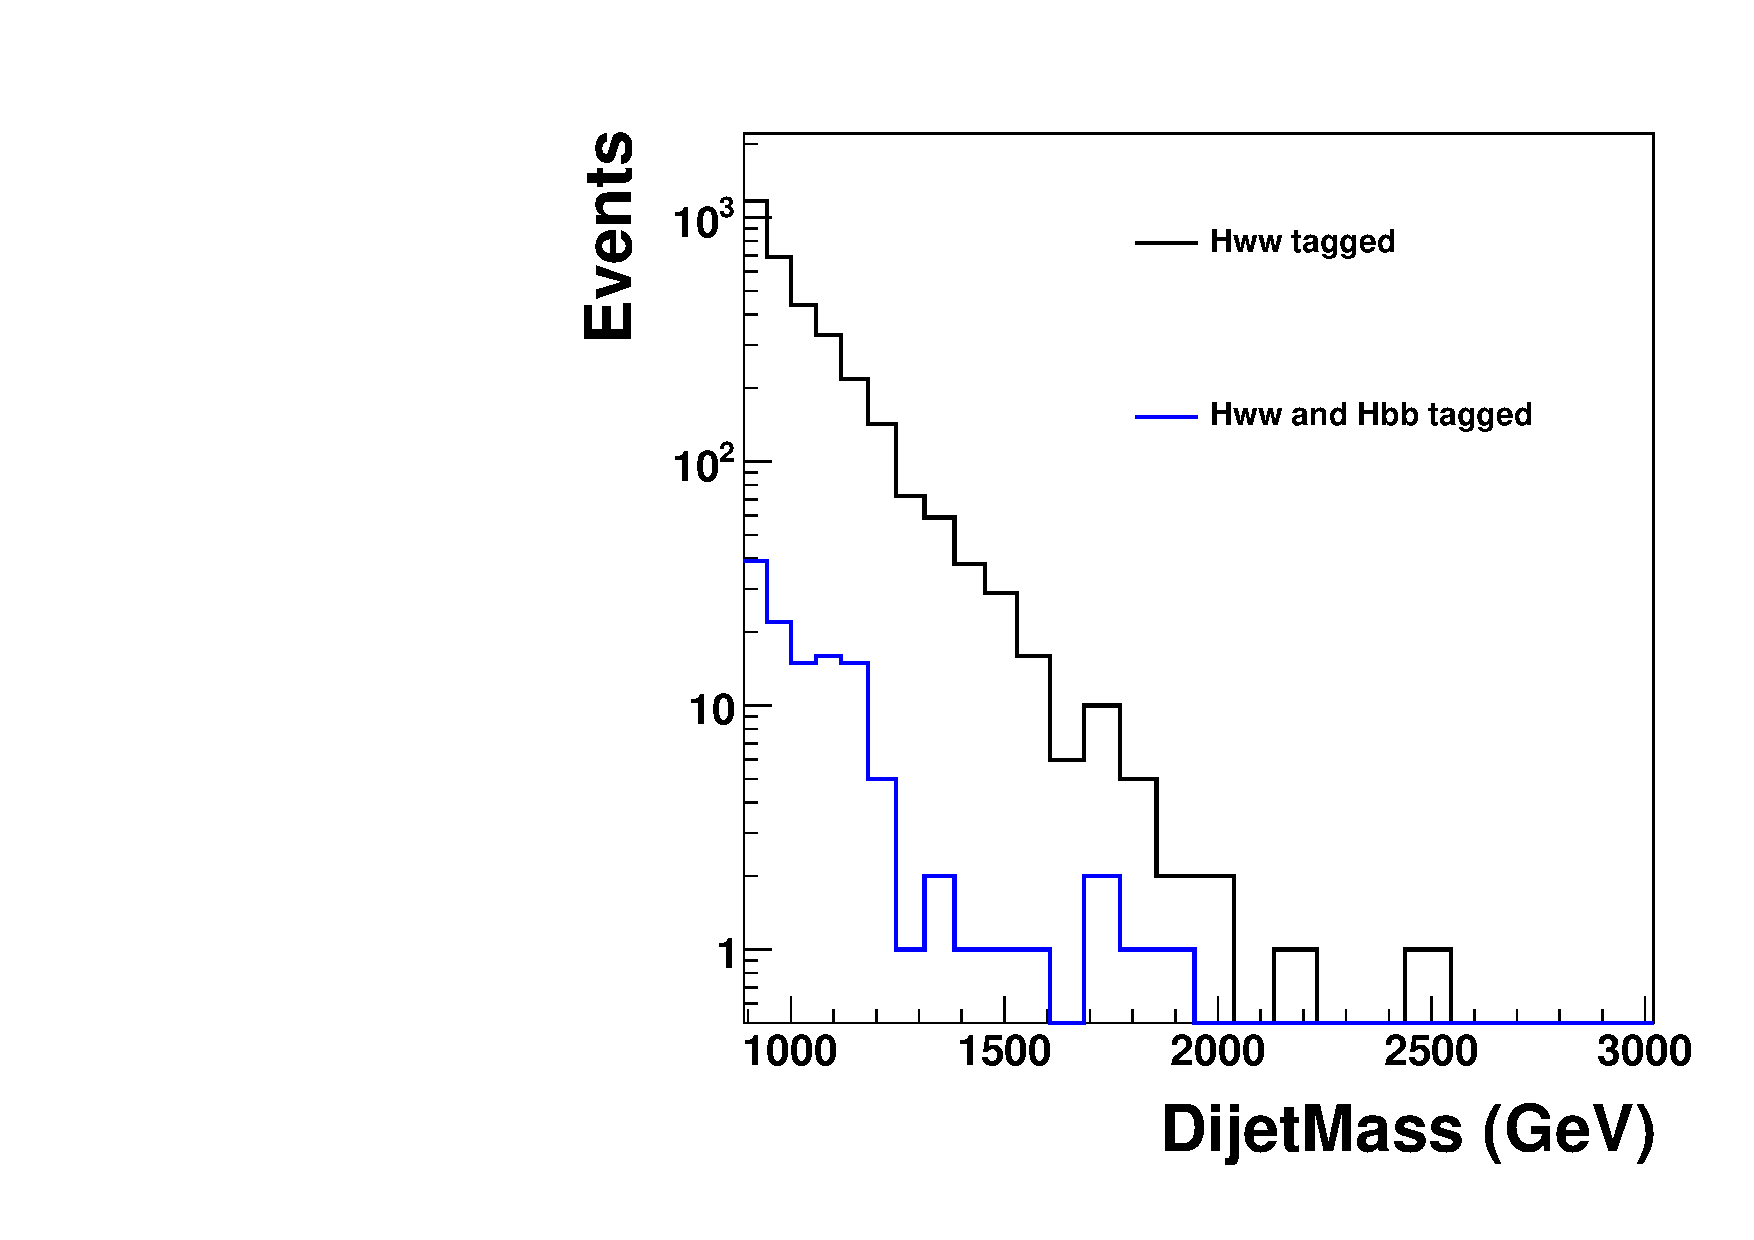
\includegraphics[width=0.49\textwidth]{HqqqqZqqfigs/HbbHww/HighPurity.pdf}
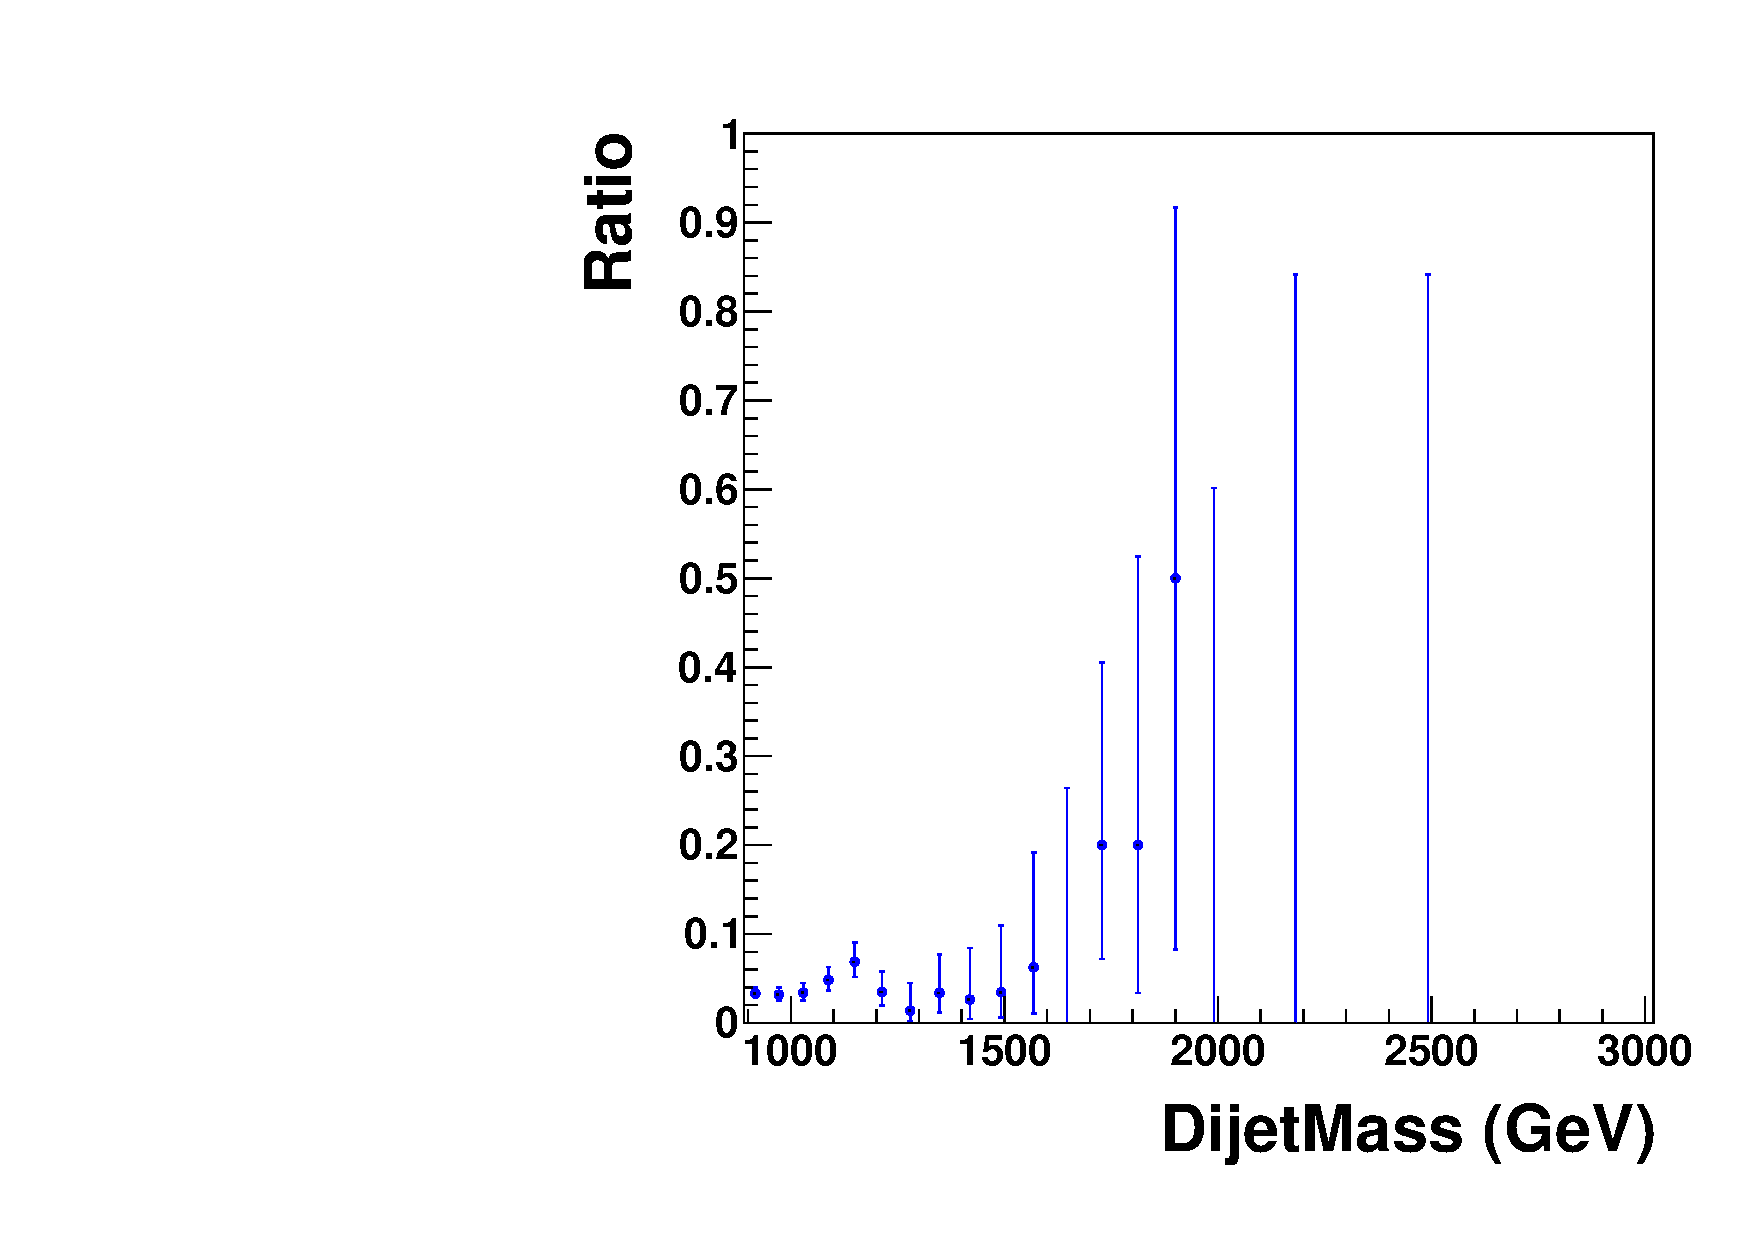
\includegraphics[width=0.49\textwidth]{HqqqqZqqfigs/HbbHww/HighPurityRatio.pdf}
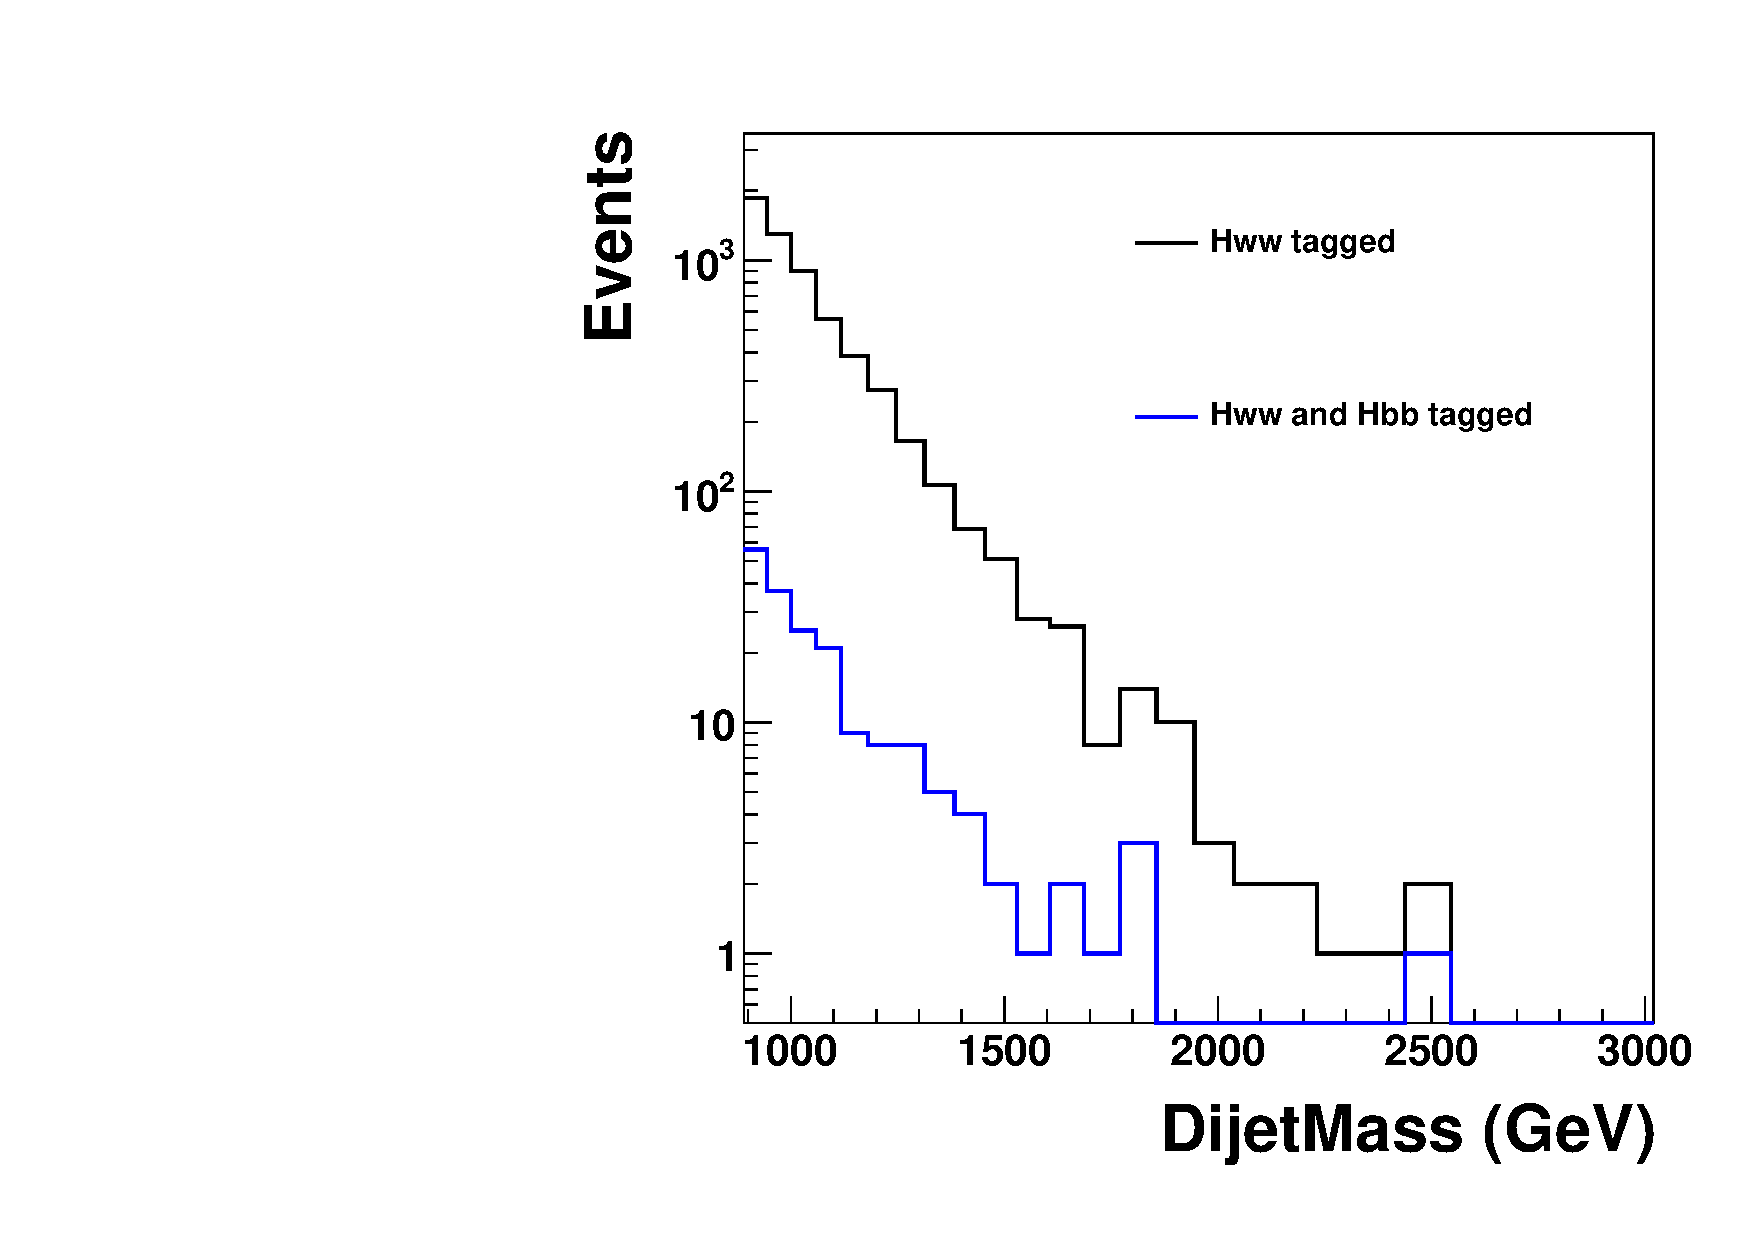
\includegraphics[width=0.49\textwidth]{HqqqqZqqfigs/HbbHww/LowHPurity.pdf}
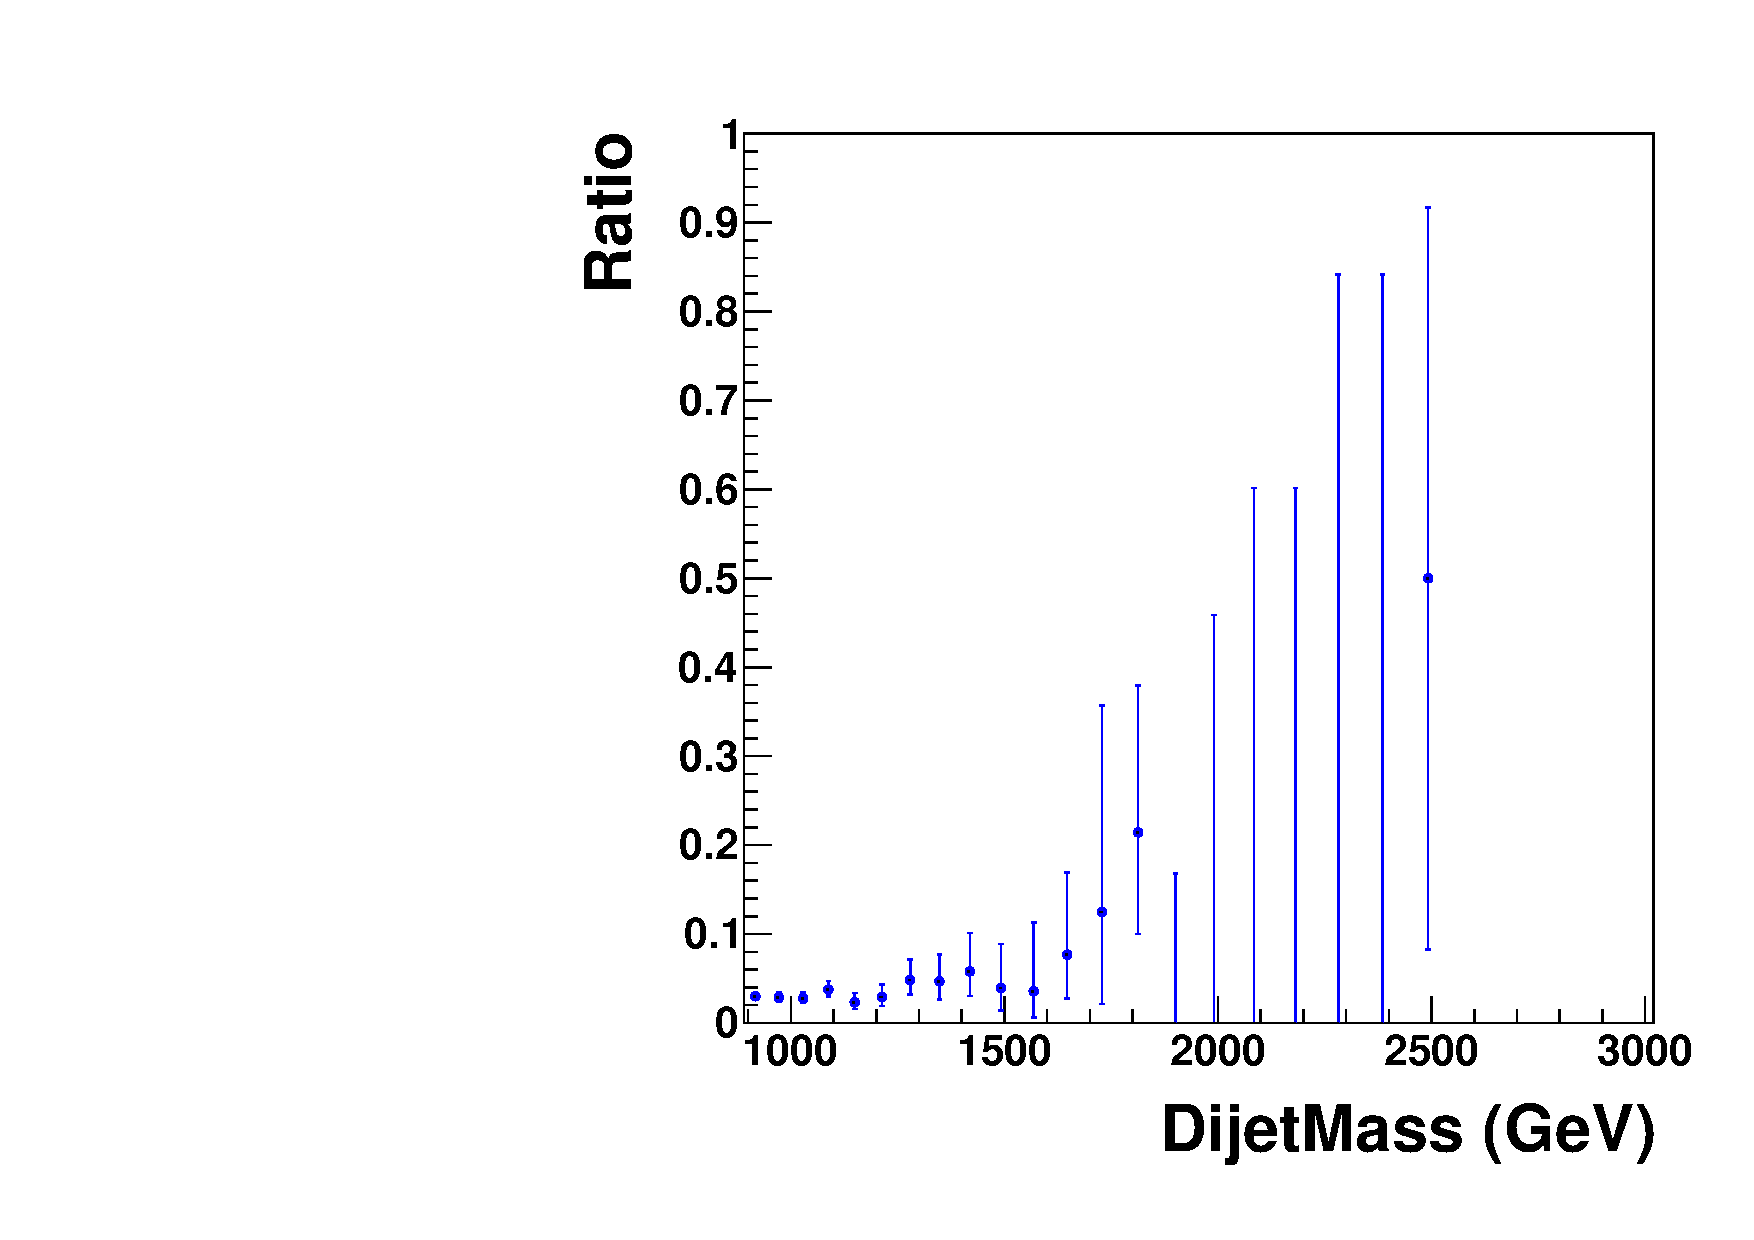
\includegraphics[width=0.49\textwidth]{HqqqqZqqfigs/HbbHww/LowHPurityRatio.pdf}
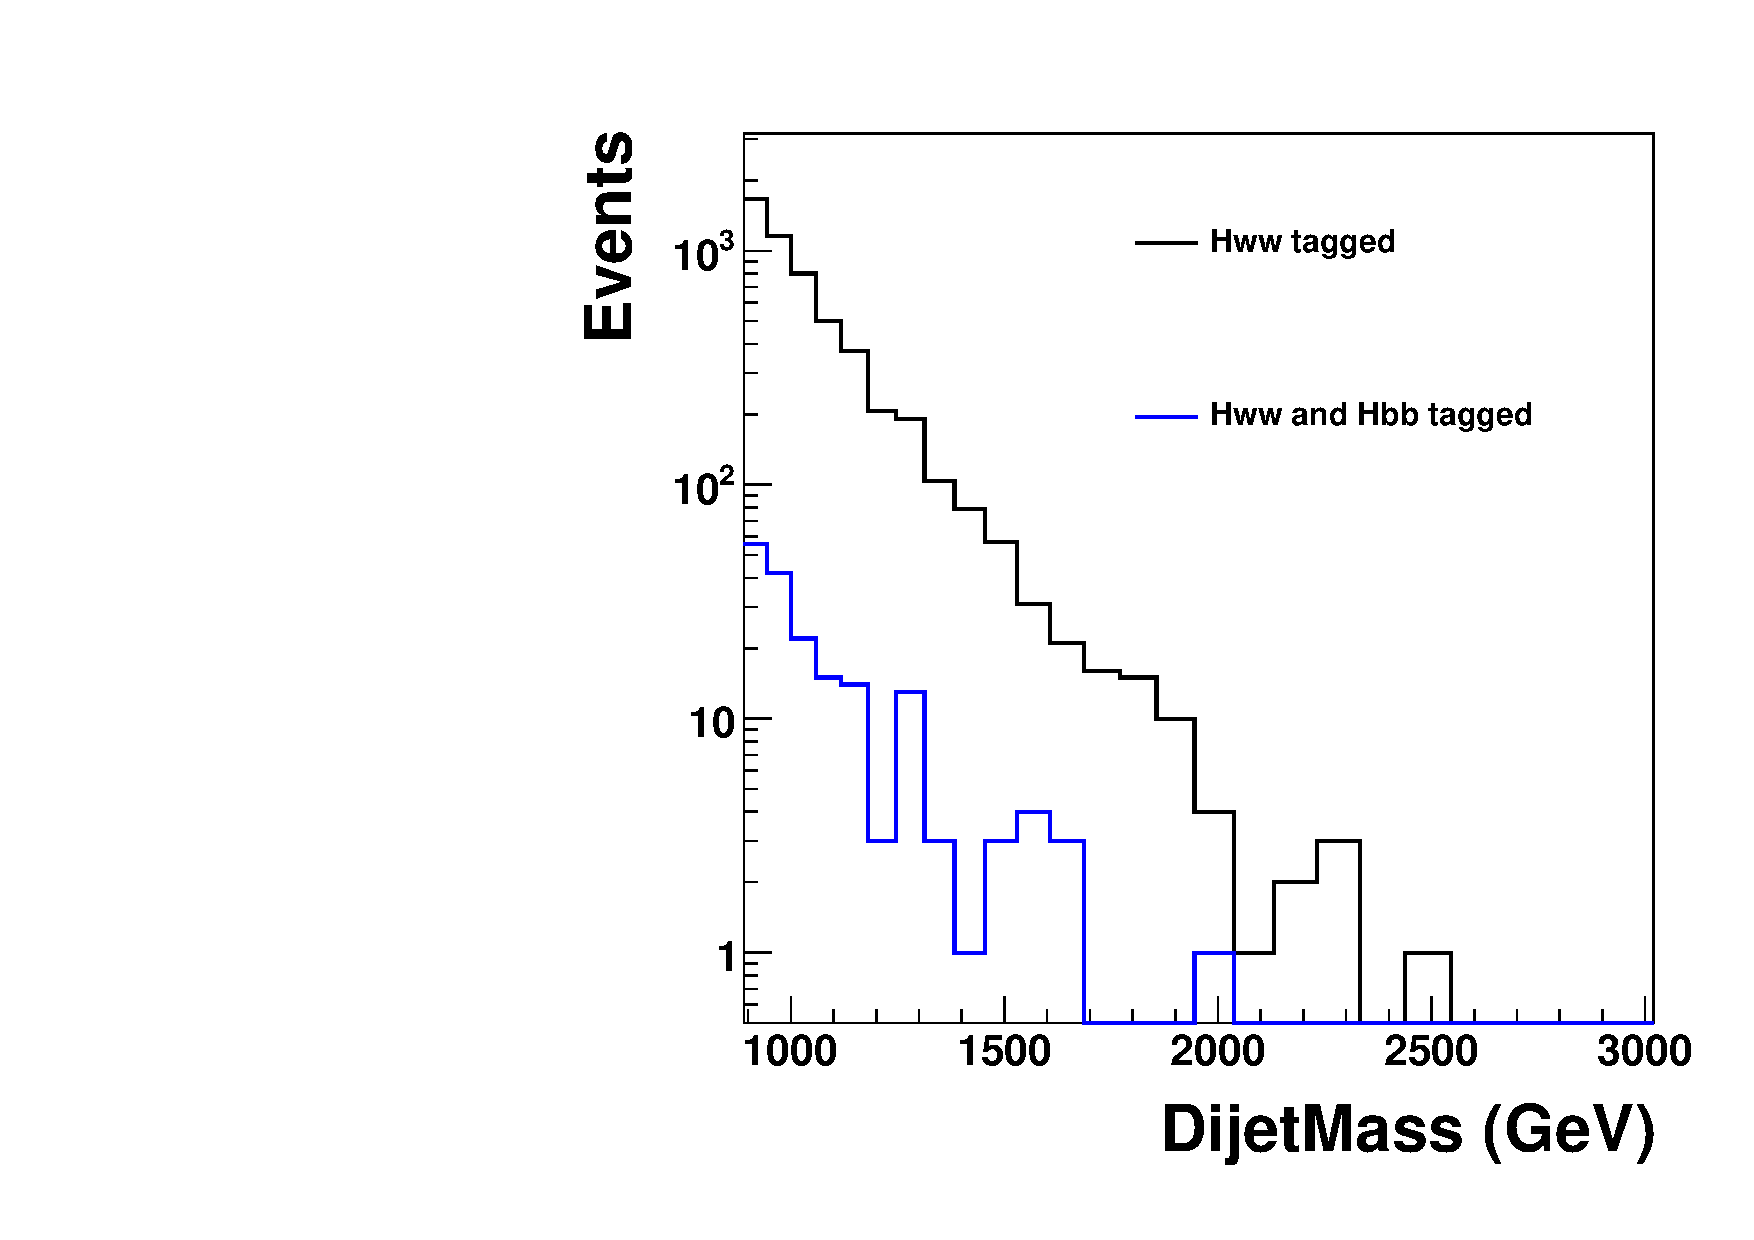
\includegraphics[width=0.49\textwidth]{HqqqqZqqfigs/HbbHww/LowVPurity.pdf}
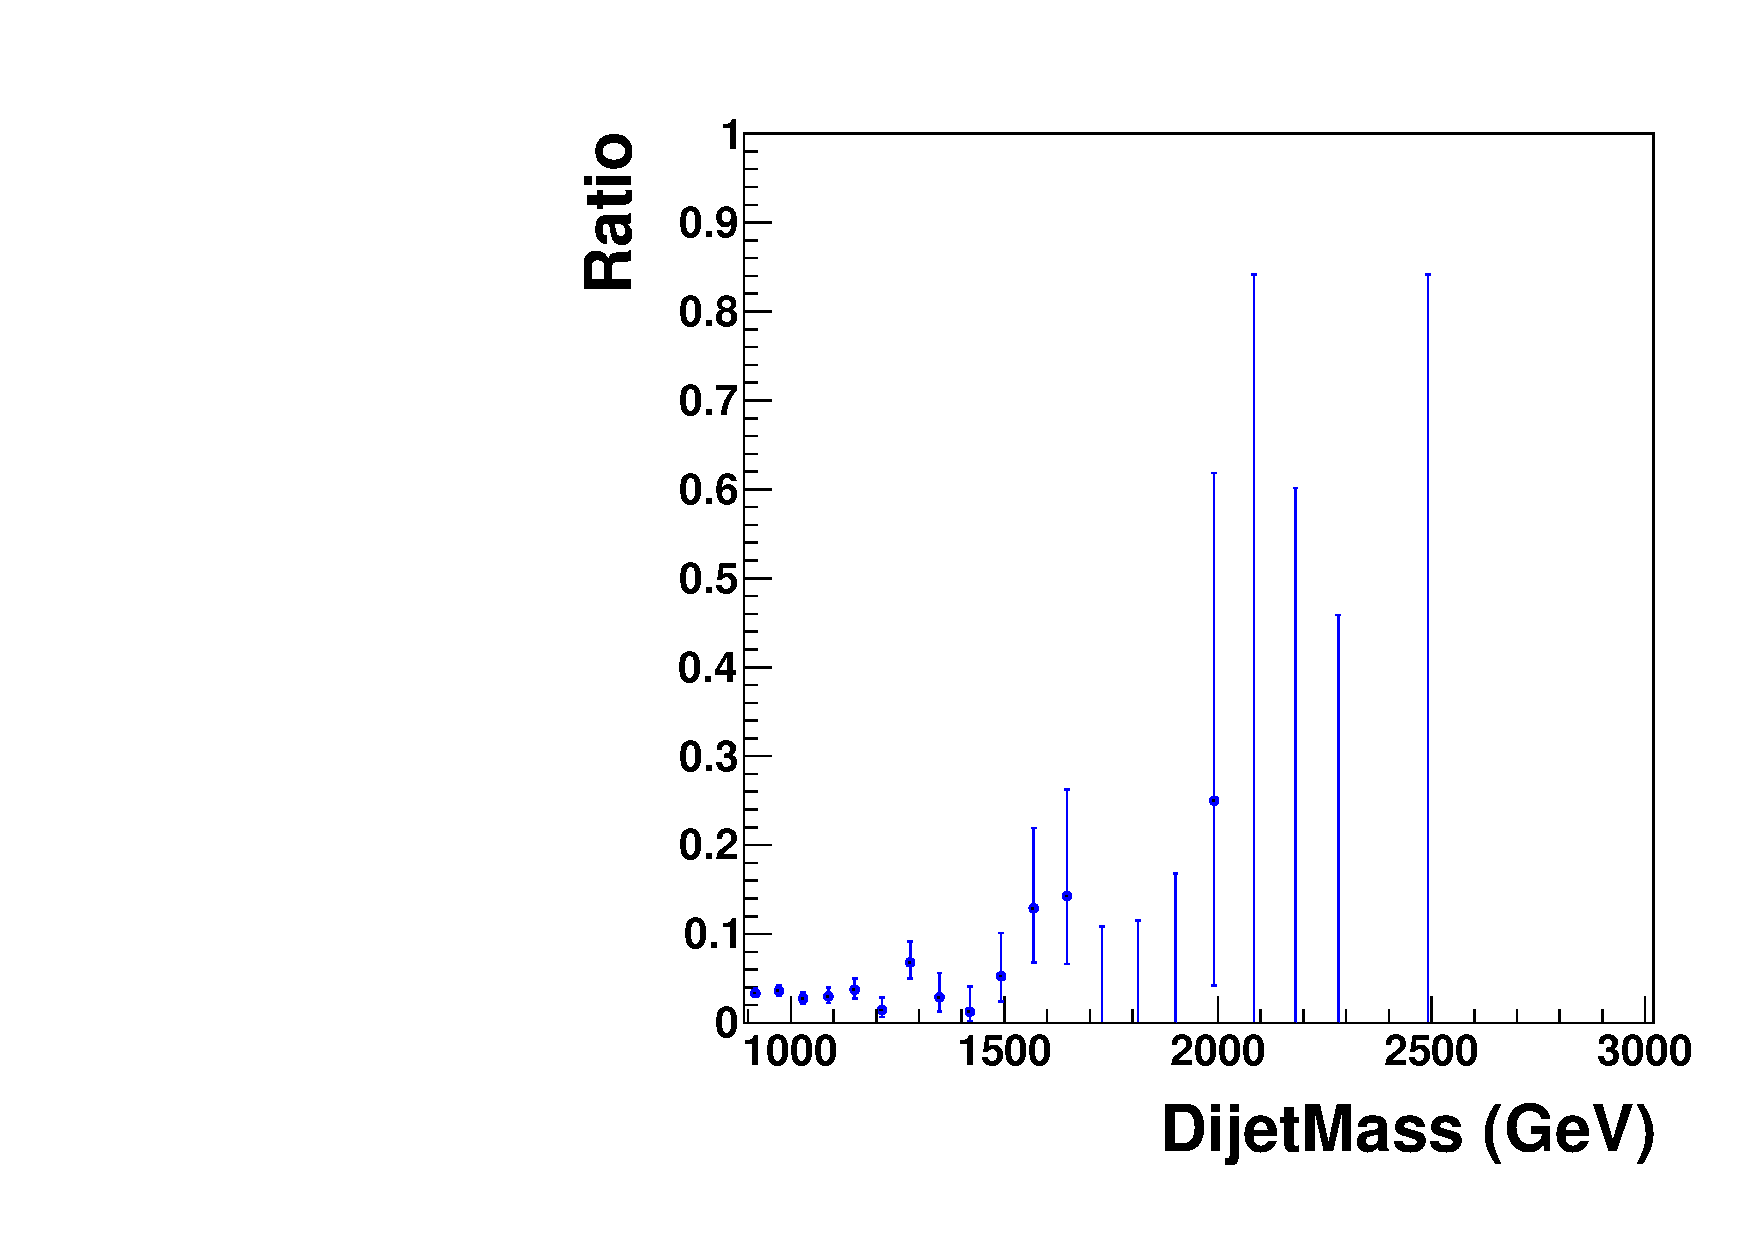
\includegraphics[width=0.49\textwidth]{HqqqqZqqfigs/HbbHww/LowVPurityRatio.pdf}
\end{center}
\caption{
Dijet mass distribution in data, for events pass Hww tagger only. And evnts pass both Hww and Hbb tagger.Plot on the top right, is the High purity Hww tagger, plots in the middle are the Low purity Hww tagger. Plots on the bottom are the low purity V tagger.  Plots on 
the right hand are the corresponding ratio(#EventsPassHbbHww/#EventsPassHww) plot.  
}
\label{fig:HbbRatio}
\end{figure}

\clearpage


\newpage
%\section{Benchmark model for a vector triplet}
%
%Information about the signal models used  is in Table~\ref{table:signalModels}

%\begin{table}[htbp]
%\resizebox{\textwidth}{!}{
%\begin{tabular}{|r|r|r|r|r|r|r|}
%\hline
%\multicolumn{1}{|l|}{M(GeV)} & \multicolumn{1}{l|}{width(GeV)} & \multicolumn{1}{l|}{BR(Z'$\to$WW)} & \multicolumn{1}{l|}{BR(Z'$\to$HZ ) } & \multicolumn{1}{l|}{BR(W'$\to$ZW)} & \multicolumn{1}{l|}{BR(W'$\to$HW )} & \multicolumn{1}{l|}{X-section(pb)} \\ \hline
%800 & 32.03 & 0.4139 & 0.5672 & 0.4287 & 0.5528 & 3.17E-01 \\ 
%900 & 32.97 & 0.4393 & 0.534 & 0.4513 & 0.5223 & 2.39E-01 \\ 
%1000 & 34.95 & 0.4506 & 0.5176 & 0.4603 & 0.5079 & 1.65E-01 \\ 
%1500 & 47.94 & 0.4665 & 0.4893 & 0.4709 & 0.4849 & 2.44E-02 \\ 
%2000 & 62.2 & 0.4698 & 0.4815 & 0.4723 & 0.4791 & 4.01E-03 \\ 
%2500 & 76.81 & 0.471 & 0.4783 & 0.4726 & 0.4767 & 7.08E-04 \\ 
%3000 & 91.57 & 0.4716 & 0.4765 & 0.4727 & 0.4754 & 1.26E-04 \\ 
%\hline
%\end{tabular}
%}
%\caption{Summary of signal models.}
%\label{table:signalModels}
%\end{table}


\section{Data and Monte Carlo samples}
\label{sec:data_and_mc_samples}


The data sample of proton-proton collisions at $\sqrt{s}=8$~\TeVcc was collected in 2012 and corresponds to
an integrated luminosity of \intlumi.
The datasets and also the certifications
used are summarized in Table~\ref{table:dataset}. 
The dijet sample is dominated by light flavored and gluon jets, which we denote as 
the "QCD background".  
%The QCD background is obtained from data by fitting an
%analytic parameterization of the dijet invariant mass distribution.

We list part of our monte carlo simulated signal(from 1 \TeVcc to 2.6 \TeVcc) 
in 
Table~\ref{table:Hww}. 
Signal samples are generated exclusively of the specific 
Higgs decay mode and W/Z decay mode. 
Model parameters and detailed cross sections are summarized in 
Appendix~\ref{appendix:modelParam}.
The matrix element is calculated with Madgraph~5.1.5.11~\cite{madgraph}. 
% in Table~\ref{table:Hbb} and 
%Table~\ref{table:Hww}, 
The signals of interest,
are showered and hadronized with 
\PYTHIA~6.426~\cite{pythia}, and \HERWIG{++} 2.5.0~\cite{herwig}, 
using simulation of the
CMS detector, based on \GEANTfour~\cite{refGEANT}. Tune
Z2*~\cite{bib_tunez1}
is used in \PYTHIA, while the version 23 tune~\cite{herwig} is used in
\HERWIG{++}. The CTEQ61L~\cite{cteq} parton distribution functions
(PDF) are used for \PYTHIA and the MRST2001~\cite{mrst} leading-order
(LO) PDF for \HERWIG{++}
%All Monte Carlo events are fully simulated and reconstructed via the Geant4-based CMS simulation
% and reconstruction software. 
%Information about the signal models used 
%is in Table~\ref{table:signalModels}
W' and Z' are generated with resonance widths
at $\approx$4\% of the resonance mass, slightly smaller than
the experimental resolution in $m_\mathrm{jj}$ for resonance masses
considered in the analysis. Samples showered from
 \PYTHIA are used in the analysis. %On the other hand, to compare
%the effect of hadronization,  \HERWIG{++} is therefore used
%to retrieve the difference.
While, samples from \HERWIG{++} are used to evaluate the systematic 
uncertainty by comparing the difference of hadronization from \PYTHIA.

%All simulated samples are passed through the standard CMS event
%reconstruction software.



%\begin{table}[htbp]
%\begin{tabular}{|r|r|r|r|r|r|r|}
%\hline
%\multicolumn{1}{|l|}{M(GeV)} & \multicolumn{1}{l|}{width(GeV)} & \multicolumn{1}{l|}{BR(Z'$\to$WW)} & \multicolumn{1}{l|}{BR(Z'$\to$HZ ) } & \multicolumn{1}{l|}{BR(W'$\to$ZW)} & \multicolumn{1}{l|}{BR(W'$\to$HW )} & \multicolumn{1}{l|}{X-section(pb)} \\ \hline
%800 & 32.03 & 0.4139 & 0.5672 & 0.4287 & 0.5528 & 3.17E-01 \\ 
%900 & 32.97 & 0.4393 & 0.534 & 0.4513 & 0.5223 & 2.39E-01 \\ 
%1000 & 34.95 & 0.4506 & 0.5176 & 0.4603 & 0.5079 & 1.65E-01 \\ 
%1500 & 47.94 & 0.4665 & 0.4893 & 0.4709 & 0.4849 & 2.44E-02 \\ 
%2000 & 62.2 & 0.4698 & 0.4815 & 0.4723 & 0.4791 & 4.01E-03 \\ 
%2500 & 76.81 & 0.471 & 0.4783 & 0.4726 & 0.4767 & 7.08E-04 \\ 
%3000 & 91.57 & 0.4716 & 0.4765 & 0.4727 & 0.4754 & 1.26E-04 \\ 
%\hline
%\end{tabular}
%\caption{Summary of signal models.}
%\label{table:signalModels}
%\end{table}



\begin{table}[htb]
\begin{center}
\begin{tabular}{ |l| }
\hline
Dataset                                 \\
\hline
/Jet/Run2012A-22Jan2013-v1/AOD  \\
/JetHT/Run2012B-22Jan2013-v1/AOD  \\
/JetHT/Run2012C-22Jan2013-v1/AOD  \\
/JetHT/Run2012D-22Jan2013-v1/AOD  \\
\hline
\end{tabular} 
\end{center}
\caption{Summary of 8~\TeVcc collision data used in this analysis. 
The certification file used for these data is 
{\tt Cert\_190456-208686\_8TeV\_22Jan2013ReReco\_Collisions12\_JSON.txt
}.
}
\label{table:dataset}
\end{table}

\begin{table}[htb]
\begin{center}
\begin{tabular}{ |l|c|r|r| }
\hline
Process     & mass ($\GeVcc$) & Events & X-sec[pb] \\
\hline
Z' $\to$ HZ & 1000   &20000   & 8.56E-02 \\
 & 1500   &20000              & 1.19E-02 \\
 & 2000   &20000              & 1.93E-03 \\
 & 2500  &20000               & 3.39E-04  \\\hline
%W' $\to$ H(ww $\to$ qqqq)W(qq)(m=750$\GeVcc$) &Madgraph   &20000   &4.071E+01  \\
W' $\to$ HW& 1000   &20000   &  1.71E-01  \\
 & 1500 &20000               &  2.55E-02  \\
 & 2000 &20000               &  4.25E-03  \\
 & 2500  &20000              &  7.31E-04  \\
\hline
\end{tabular}
\end{center}
\caption{Examples of the simulated Monte Carlo samples used in this analysis for process
 V' $\to$ VH. Cross sections are calculated from 
production cross sections of V' times its BR(W' $\to$HW or Z' $\to$ HZ). 
 These samples are generated using Madgrap5 and hadronized with Pythia6. }
\label{table:Hww}
\end{table}


\iffalse

\begin{table}[htb]
\begin{center}
\begin{tabular}{ |l|c|r|r| }
\hline
Process           & mass ($\GeVcc$) & Events & X-sec[pb] \\
\hline
Z' $\to$ H(bb)Z(qq) & 1000  &20000   & 3.45E-02 \\
 & 1500     &20000   & 4.81E-03 \\
 & 2000    &20000   & 7.79E-04  \\
 & 2500    &20000   & 1.37E-04 \\\hline
%W' $\to$ H(bb)W(qq)(m=750$\GeVcc$) &Madgraph   &20000   &4.071E+01  \\
W' $\to$ H(bb)W(qq)& 1000  &20000   & 3.28E-02 \\
 & 1500    &20000   & 4.61E-03 \\
 & 2000    &20000   & 7.50E-04 \\
 & 2500     &20000   & 1.32E-04 \\
\hline
\end{tabular}
\end{center}
\caption{Examples of the simulated Monte Carlo samples used in this analysis for process
 Z'/W'$\to$Z/W(qq) + H(bb). Those samples was generated using Madgrap5 and hadronized with Pythia6.}
\label{table:Hbb}
\end{table}

\begin{table}[htb]
\begin{center}
\begin{tabular}{ |l|c|r|r| }
\hline
Process     & mass ($\GeVcc$) & Events & X-sec[pb] \\
\hline
Z' $\to$ H(ww $\to$ qqqq)Z(qq) & 1000   &20000   & 5.88E-03 \\
 & 1500   &20000   & 8.19E-04 \\
 & 2000   &20000   & 1.33E-04 \\
 & 2500  &20000   & 2.33E-05 \\\hline
%W' $\to$ H(ww $\to$ qqqq)W(qq)(m=750$\GeVcc$) &Madgraph   &20000   &4.071E+01  \\
W' $\to$ H(ww $\to$ qqqq)W(qq)& 1000   &20000   & 5.58E-03 \\
 & 1500 &20000   & 7.85E-04  \\
 & 2000 &20000   & 1.28E-04 \\
 & 2500  &20000   & 2.24E-05 \\
\hline
\end{tabular}
\end{center}
\caption{Examples of the simulated Monte Carlo samples used in this analysis for process
 Z'/W'$\to$Z/W(qq) + H(ww $\to$ qqqq). Those samples was generated using Madgrap5 and hadronized with Pythia6.}
\label{table:Hww}
\end{table}

\fi



\newpage

\section{Trigger}
\label{sec:trigger}


Events are selected if one of the following triggers has fired: HLT\_HT750, HLT\_PFHT650, HLT\_PFNoPUHT650,
HLT\_FatDiPFJetMass750\_DR1p1\_Deta1p5.  All versions of each of these triggers are used. None of these triggers are prescaled druing the 2012 data taking period. HLT\_PFNoPUHT650 trigger is used for the data set after the RunC(including RunC), while HLT\_PFHT650
trigger is only used for RunA and RunB data sets. 


Figure~\ref{fig:trigger efficiencies part1}, Figure~\ref{fig:trigger efficiencies part2}, and Figure~\ref{fig:trigger efficiencies part3} show the trigger efficiencies of the OR of the highest threshold HLT\_PFHT650 trigger and the HLT\_FatJetMass trigger w.r.t. an OR of the lower threshold HLT\_HT550 trigger. From the plot, the trigger is $99\%$ effiecient above 890\GeVcc for the untagged, single tagged and double tagged data. 


\begin{figure}[htb]
\centering
     \resizebox{0.75\linewidth}{!}{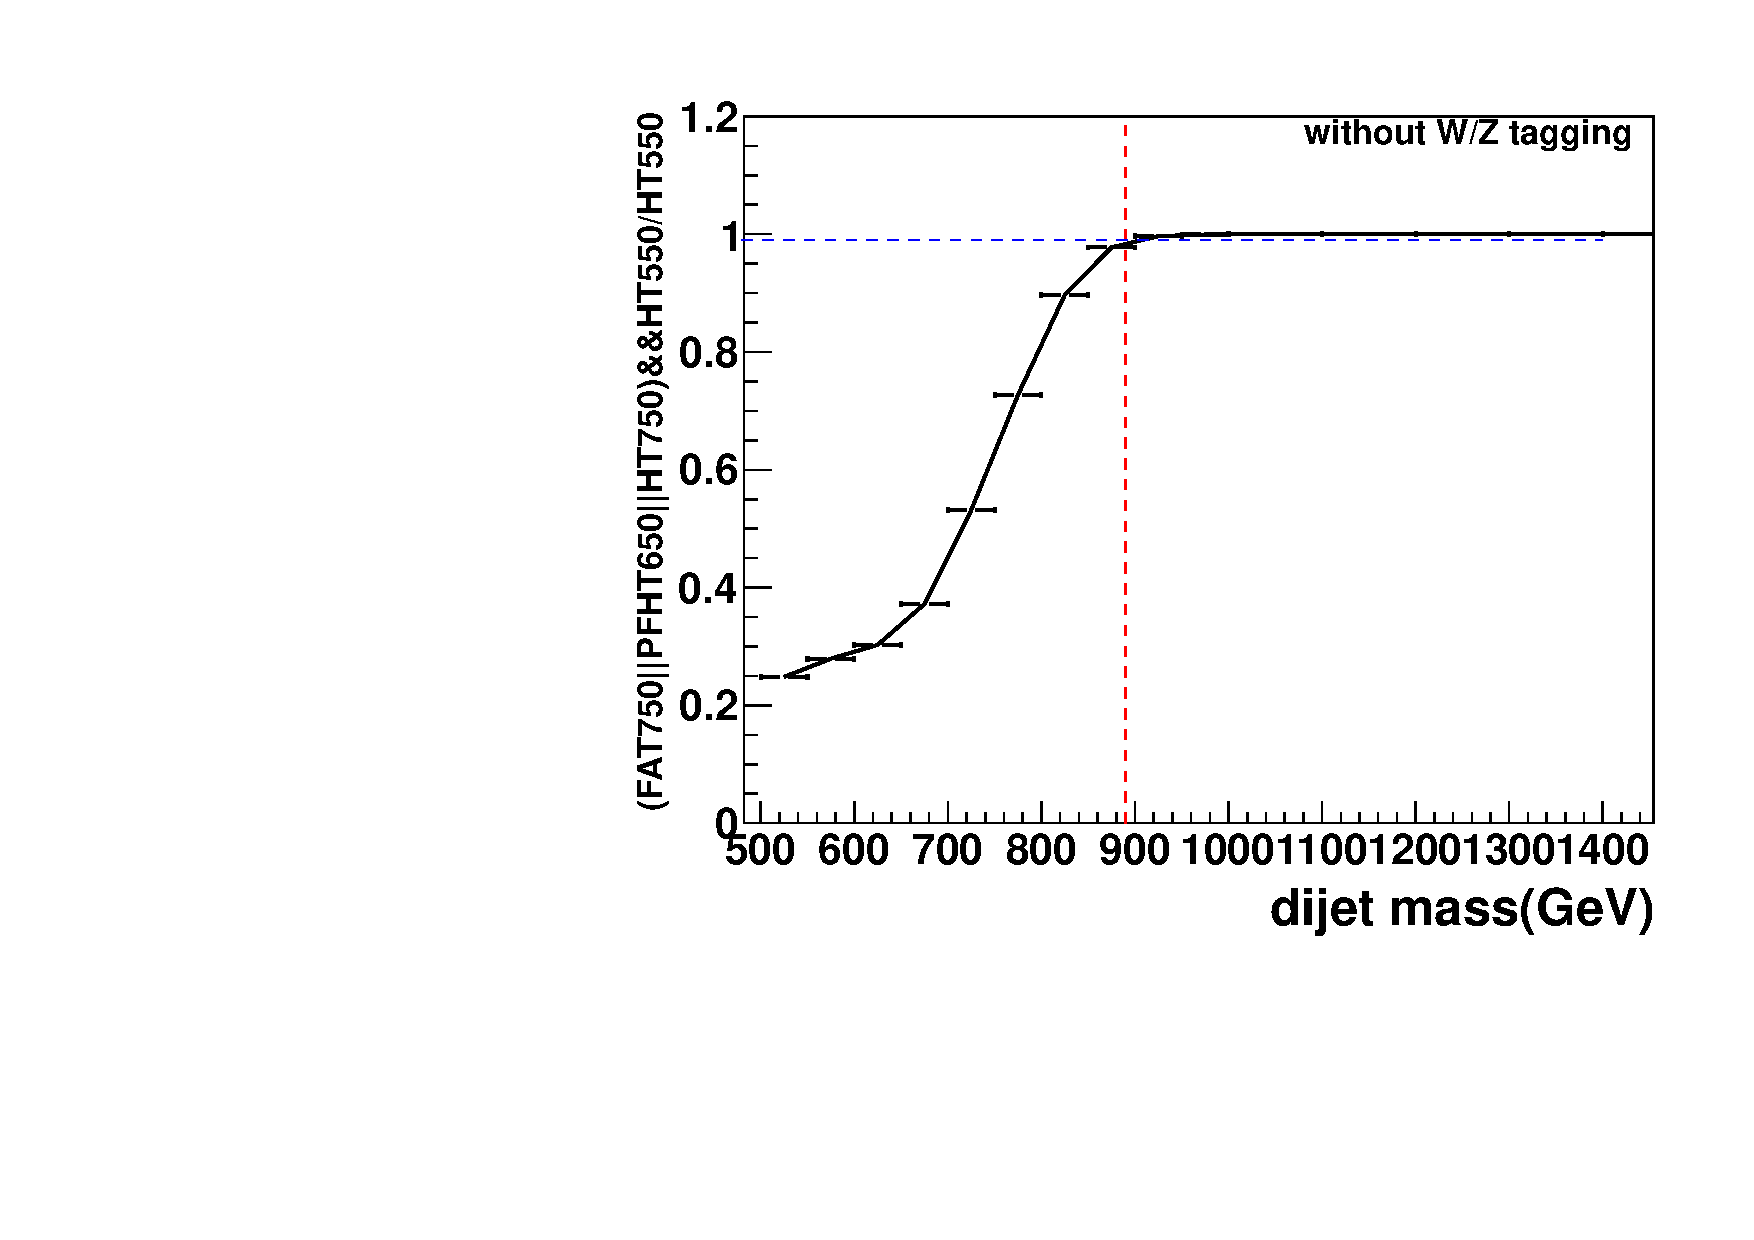
\includegraphics{EXO-12-024/figs/trigger-eff/Dataeff_withouttagging.pdf}} \\   
\caption[Trigger efficiencies]{Trigger efficiency for untagged data of FAT\_750$\parallel$HLT\_PF(NoPU)HT650$\parallel$HLT\_HT750 measured using data collected by lower threshold $H_T550$ trigger. The dash red line is positioned at $m_{jj}$ equal $890 GeV$, the blue line is at efficiency at 99$\%$. }
  \label{fig:trigger efficiencies part1}
\end{figure}

\begin{figure}[htb]
\centering
     \resizebox{0.75\linewidth}{!}{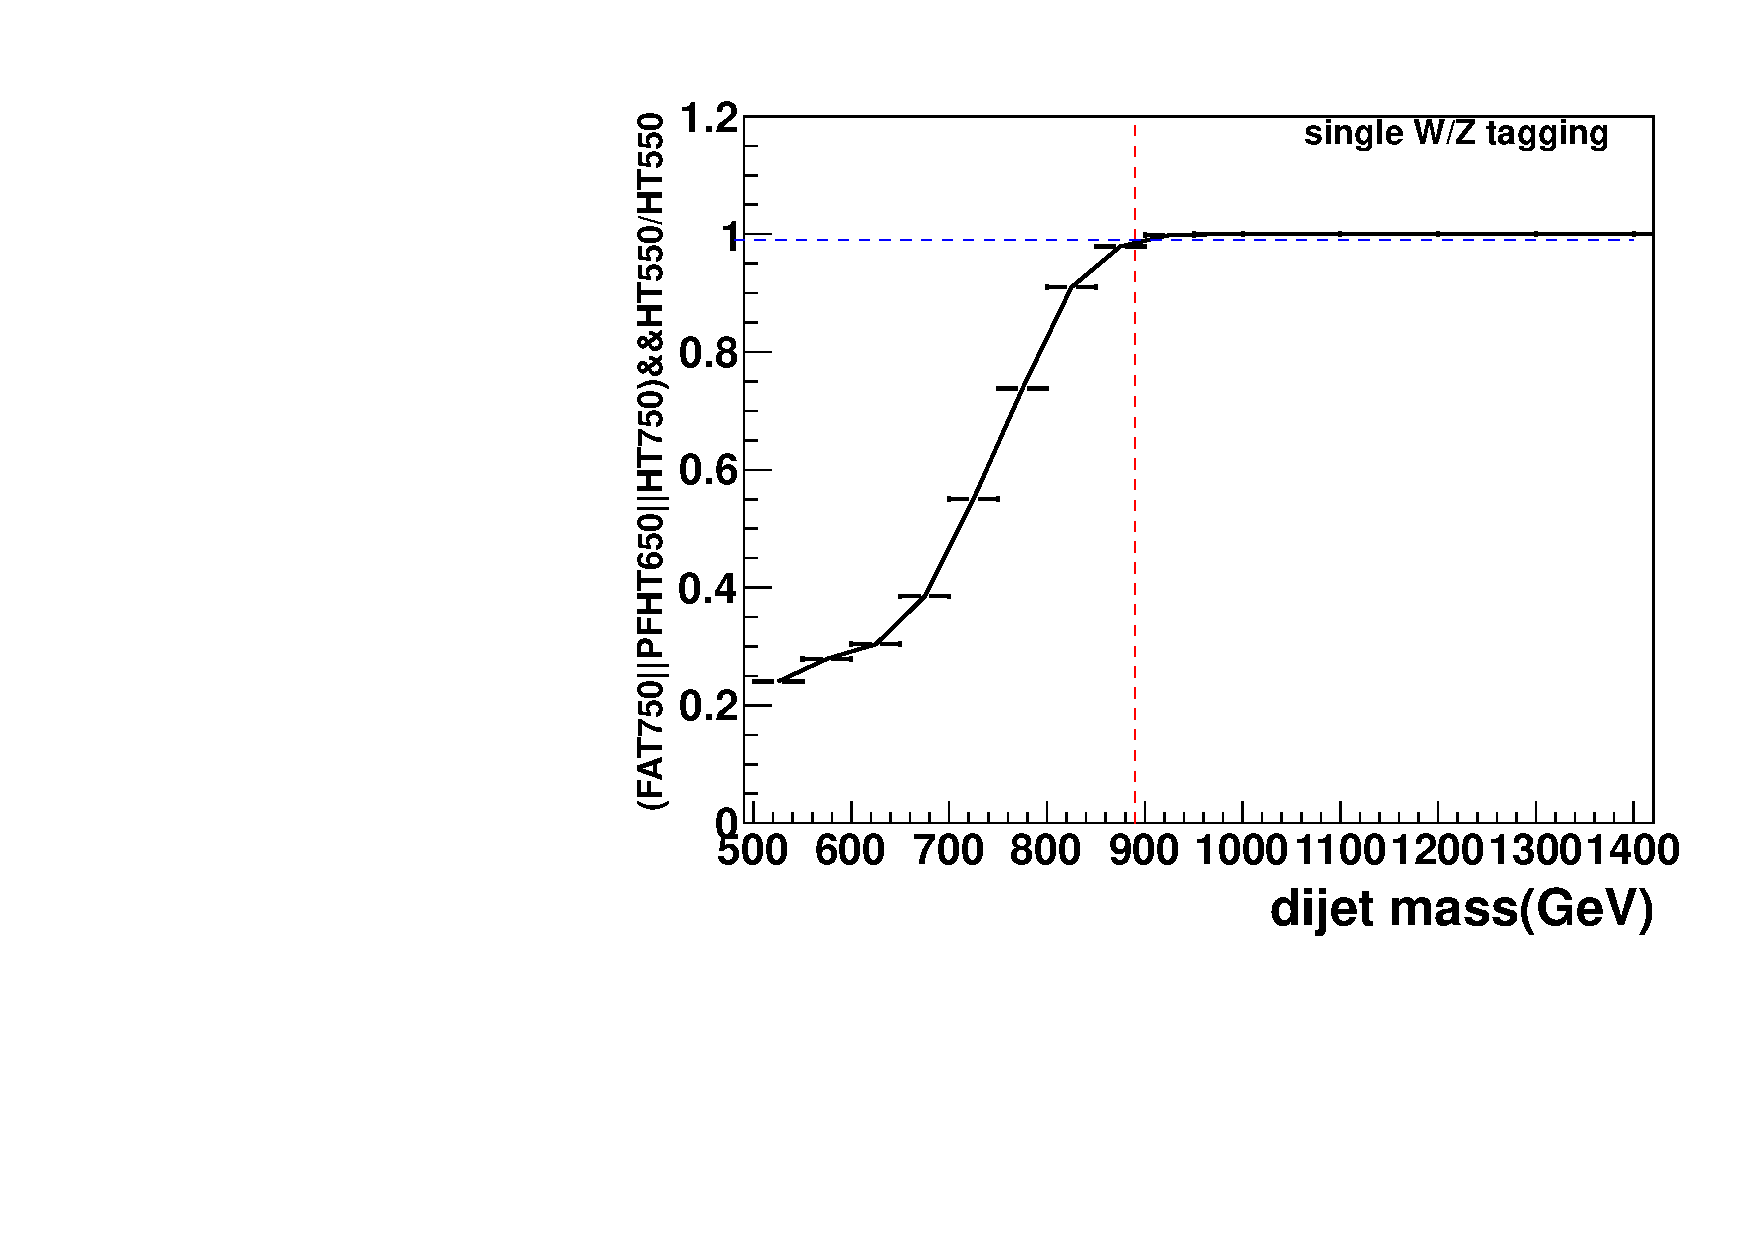
\includegraphics{EXO-12-024/figs/trigger-eff/Dataeff_singletagging.pdf}}  \\
\caption[Trigger efficiencies]{Trigger efficiency for single tagged data of FAT\_750$\parallel$HLT\_PF(NoPU)HT650$\parallel$HLT\_HT750 measured using data collected by lower threshold $H_T550$ trigger. The dash red line is positioned at $m_{jj}$ equal $890 GeV$, the blue line is at efficiency at 99$\%$. }
  \label{fig:trigger efficiencies part2}
\end{figure}

\begin{figure}[htb]
\centering
     \resizebox{0.75\linewidth}{!}{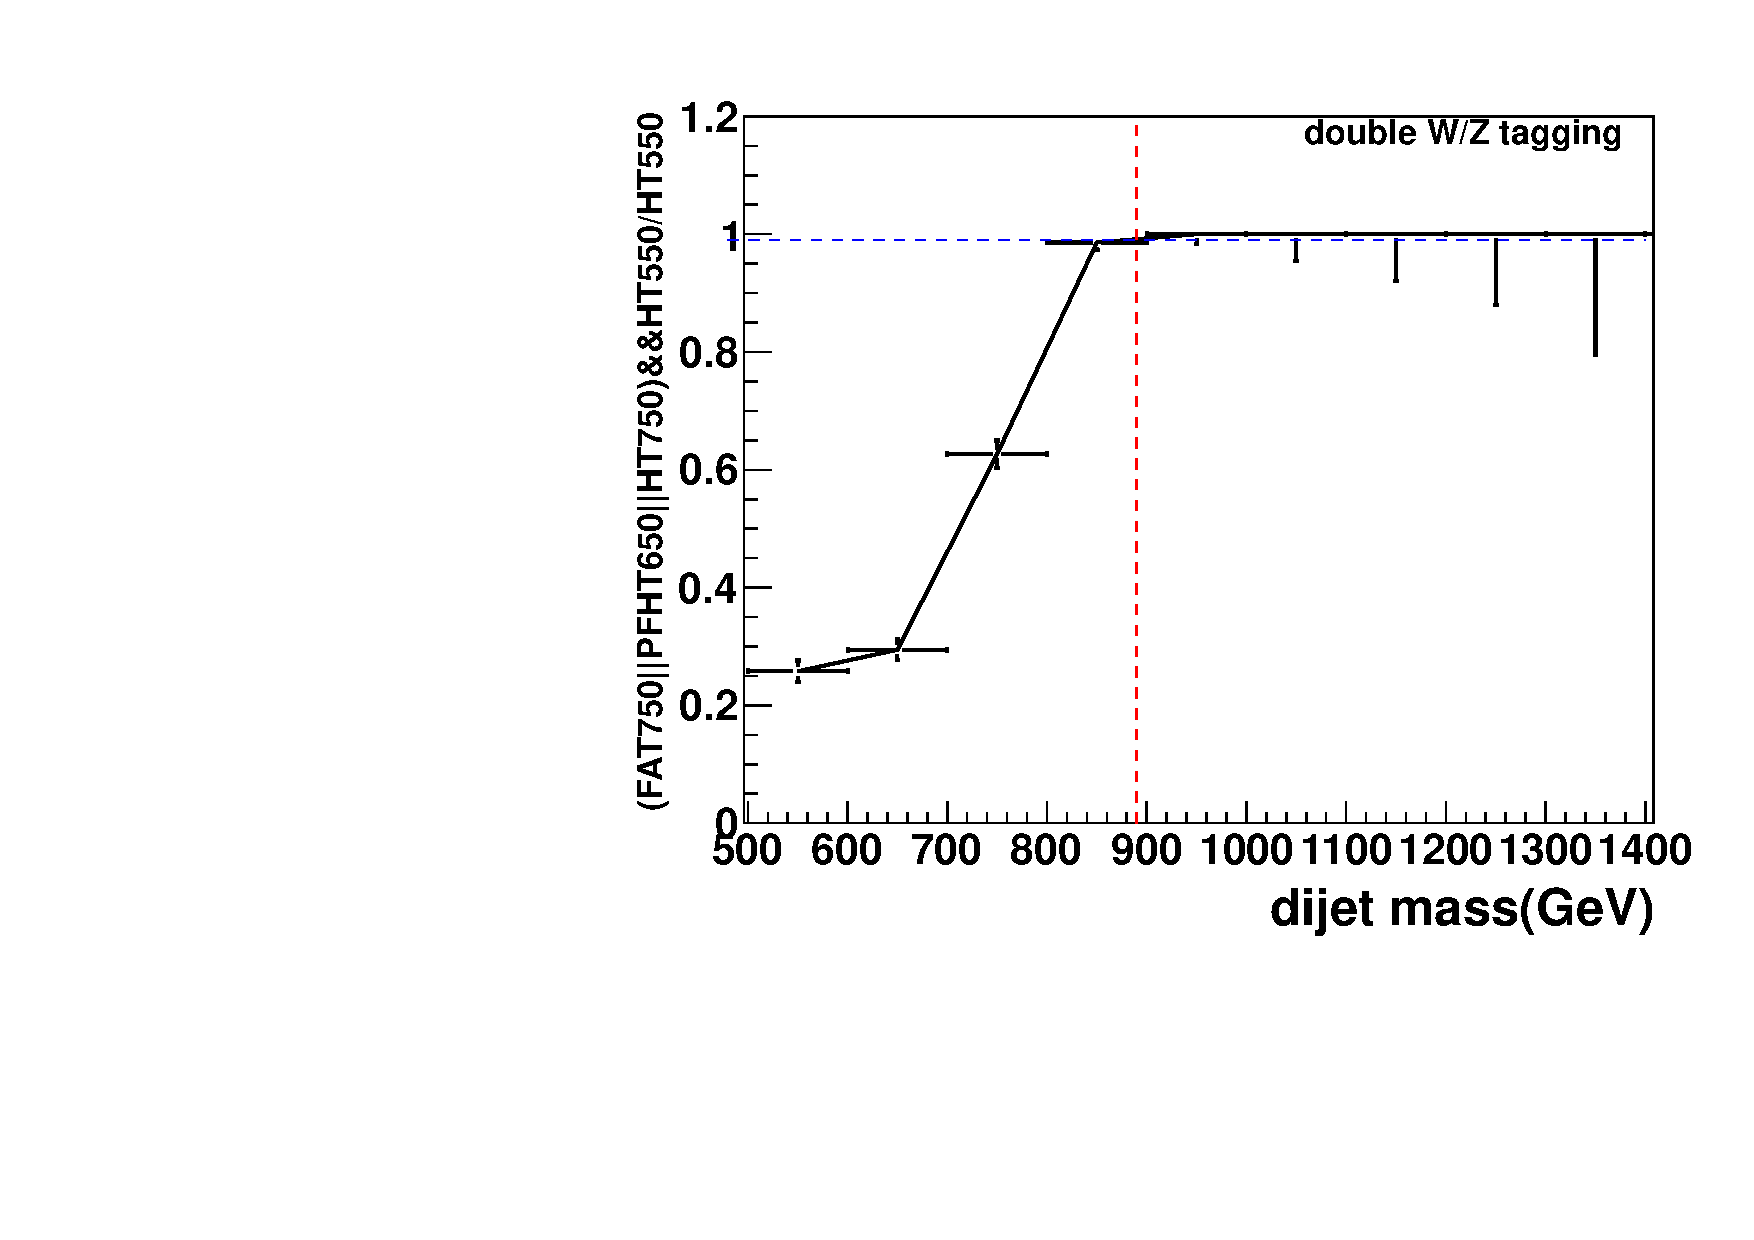
\includegraphics{EXO-12-024/figs/trigger-eff/Dataeff_doubletagging.pdf}} \\
\caption[Trigger efficiencies]{Trigger efficiency for double tagged data of FAT\_750$\parallel$HLT\_PF(NoPU)HT650$\parallel$HLT\_HT750 measured using data collected by lower threshold $H_T550$ trigger. The dash red line is positioned at $m_{jj}$ equal $890 GeV$, the blue line is at efficiency at 99$\%$. }
  \label{fig:trigger efficiencies part3}
\end{figure}


\clearpage














\section{Event preselection}
\label{sec:analysisEXO-14-009}


The event reconstruction adopt the same algorithm and procedure as
Section~\ref{sec:analysis1} in Chapter~\ref{chap:chapter3}. For details, please refer to that section.  





%\section{The W/Z-Tagging algorithm}
\label{sec: W/Z tagging1}

The products of hadronic decays of W bosons can
fall within a single jet if these particles are boosted relative to
their mass.  The W tagging algorithm is developed to
identify these boosted W jets, based on the removal of the softest
components of the jets (jet pruning)~\cite{catop_cms,topwtag_pas}.

 Jet pruning is implemented as application of additional cuts in the process
of CA jet clustering. This algorithm starts from a set of ``protojets" given by the PF particles
that form the original CA jet within a cone of R = 0.8. As in the standard CA jet clustering,
these protojets are iteratively combined with each other until all jets is found; however, here
the large angle and low pT protojets are removed in the process. 
%The jet pruning algorithm uses the CA $R=0.8$ jets
%as inputs. In the process, soft and
%wide-angle particles (relative to the parent in the clustering) are
%ignored.  
The same parameters are chosen for the jet pruning algorithm
as in the original theoretical papers~\cite{jetpruning1,jetpruning2}.

The following selection is then applied on the pruned jets
to identify jets from hadronic W/Z decays:

\begin{itemize}

\item {\bf Pruned jet mass}  $\mbox{\boldmath$m_{\text{jet}}$}$
  - Require the total pruned jet mass to satisfy $70 < m_\text{jet} < 100$~GeV.

\item {\bf N-subjettiness} 
  - Require the 2-subjettiness/1-subjettiness ($\tau_{2}/\tau_{1}$) $< $0.5 for the ungroomed CA8 jets. (N-subjettiness will be introduced in next section.)
\end{itemize}

A detailed performance study of this W-tagger has been made public in Reference~\cite{JME-13-006}.

\subsection{N-subjettiness}
\label{sec:N-subjettiness1}

N-subjettiness~\cite{Thaler:2010tr,Thaler:2011gf,Stewart:2010tn} exploits the fact that the pattern of the hadronic decay of a heavy object is reflected through the presence of distinctive energy lobes corresponding to the decay products, as opposed to QCD jets which present a more uniformly spread energy configuration (not aligned along the subjet axis). The inclusive jet shape N-subjettiness is defined, in its generalized version as derived in Reference~\cite{Thaler:2010tr}, as 
%
\begin{equation}
\tau_N = \frac{1}{d_{0}} \sum_{k} p_{T,k}\,min( (\Delta R_{1,k})^{\beta}, (\Delta R_{2,k})^{\beta}...(\Delta R_{N,k})^{\beta})
\end{equation}
%
where the index $k$ runs over the jet constituents and the distances
$\Delta R_{n,k}$ are calculated with respect to the axis of the $n^{\mathrm{th}}$
subjet. The normalization factor $d_{0}$ is calculated as $d_{0}=
\sum_{k} p_{T,k}R^{\beta}_{0}$, setting $R_{0}$ to the jet radius of
the original jet. In the analysis, the N-subjettiness is calculated
from the ungroomed jets with the parameter $\beta=1$. In particular,
the variable able to best discriminate between $\PW/\cPZ$ jets and QCD jets
is the ratio of 2-subjettiness over 1-subjettiness,
$\tau_{21}=\tau_{2} / \tau_{1}$, which turns out to be smaller for signal than for background as demonstrated in Figure~\ref{fig:N-sub-mass}.

\begin{figure}[htb]
\centering
\begin{tabular}{cc}
     \resizebox{0.5\linewidth}{!}{\includegraphics{EXO-12-024/figs/N-subjettiness/Signal_MC_Pre.pdf}} &
     \resizebox{0.5\linewidth}{!}{\includegraphics{EXO-12-024/figs/N-subjettiness/Signal_MC.pdf}} \\
\end{tabular}
\caption[N-subjettiness]{Comparison for $\tau_{2}/\tau_{1}$ distribution between signal (red) and background (black) before the jet mass cut (left) and after the jet mass cut applied (right). The signal MC used here is Herwig WW 1.5 TeV, and background is Herwig QCD.}
\label{fig:N-sub-mass}
\end{figure}

%\textbf{PLAN} in Fig~\ref{N-sub} and Fig~\ref{N-sub-mass}, I'm gonna add prettier plots for different signals(pythia and herwig, 1.0Tev to 3.0TeV resonance).  

%The leading two ungroomed CA8 jets to the leading two pruned CA8 jets are matched requireing $\Delta R < 0.5 $, which fails in less than 0.1\% of the events.

We select ``high purity'' $\PW/\cPZ$ jets by
requiring $\tau_{21} \leq 0.5$, while $ 0.5 <
\tau_{21} < 0.75$ defines the ``low purity'' $\PW/\cPZ$ jets.
%
The division of events with one $\PW/\cPZ$-tag follows the same delineation.
%
The events with two $\PW/\cPZ$-tagged jets are always required 
to have one high purity $\PW/\cPZ$ tag, and are similarly divided
into the ``high'' and the ``low purity'' categories depending on whether
the other $\PW/\cPZ$-tagged jet has passed the high or the low purity requirement, 
respectively.
%
The high purity category has been optimized to reach on average the
best sensitivity for all models considered in this search.  The low
purity category adds sensitivity in particular at high dijet masses
where the $\PW/\cPZ$-tagging efficiency drops along with the
background rate.

\subsection{Optimization study for the W-tagger}
\label{sec:optimal}
%\textbf{PLAN} This part we're gonna talk about what we did for the optimization search of tau2/tau1 cut. 

The cut values for the pruned jet mass and N-subjettiness were optimized based on the best expected limit.
The final cut values are a compromise between best expected limits for WW and ZZ resonances in the range between 1 and 2 TeV, because we target both of them with the same analysis.

Figure~\ref{fig:optimization0} shows the optimization of the N-subjettiness ($\tau_{21}$) or massdrop ($\mu$) cut value.
The massdrop variable was used in the 2011 version of this analysis and has been replaced by the 
N-subjettiness.
A N-subjettiness cut gives a 30\% better limit than the massdrop cut.
The $\tau_{21}<0.5$ is the best cut value for equal performance in both WW and ZZ resonances.
The expected limit changes by $<$5\% changing the $\tau_{21}$ cut value by $\pm$0.05.

\begin{figure}[htb]
\centering
\begin{tabular}{cc}
     \resizebox{0.5\linewidth}{!}{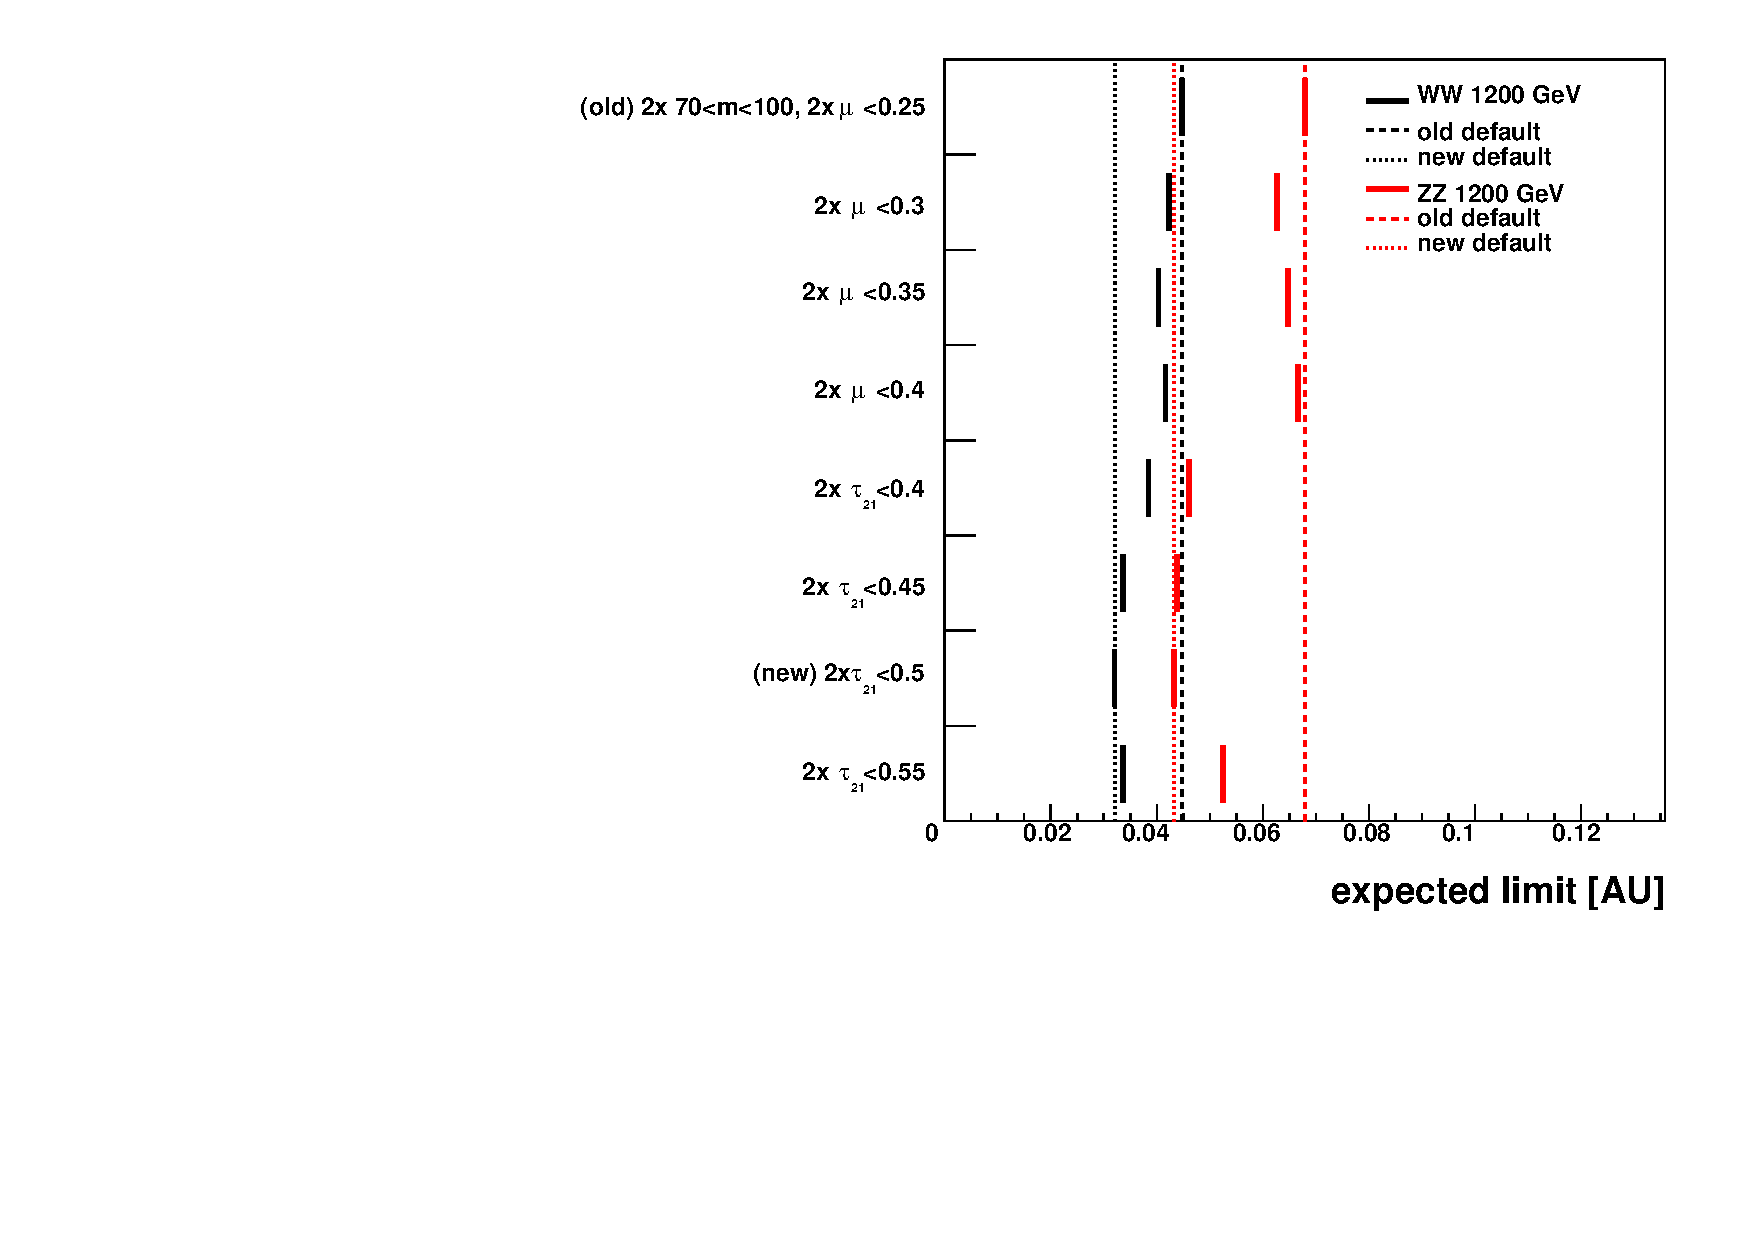
\includegraphics{EXO-12-024/figs/N-subjettiness/optimization1200_0.pdf}} &
%     \resizebox{0.5\linewidth}{!}{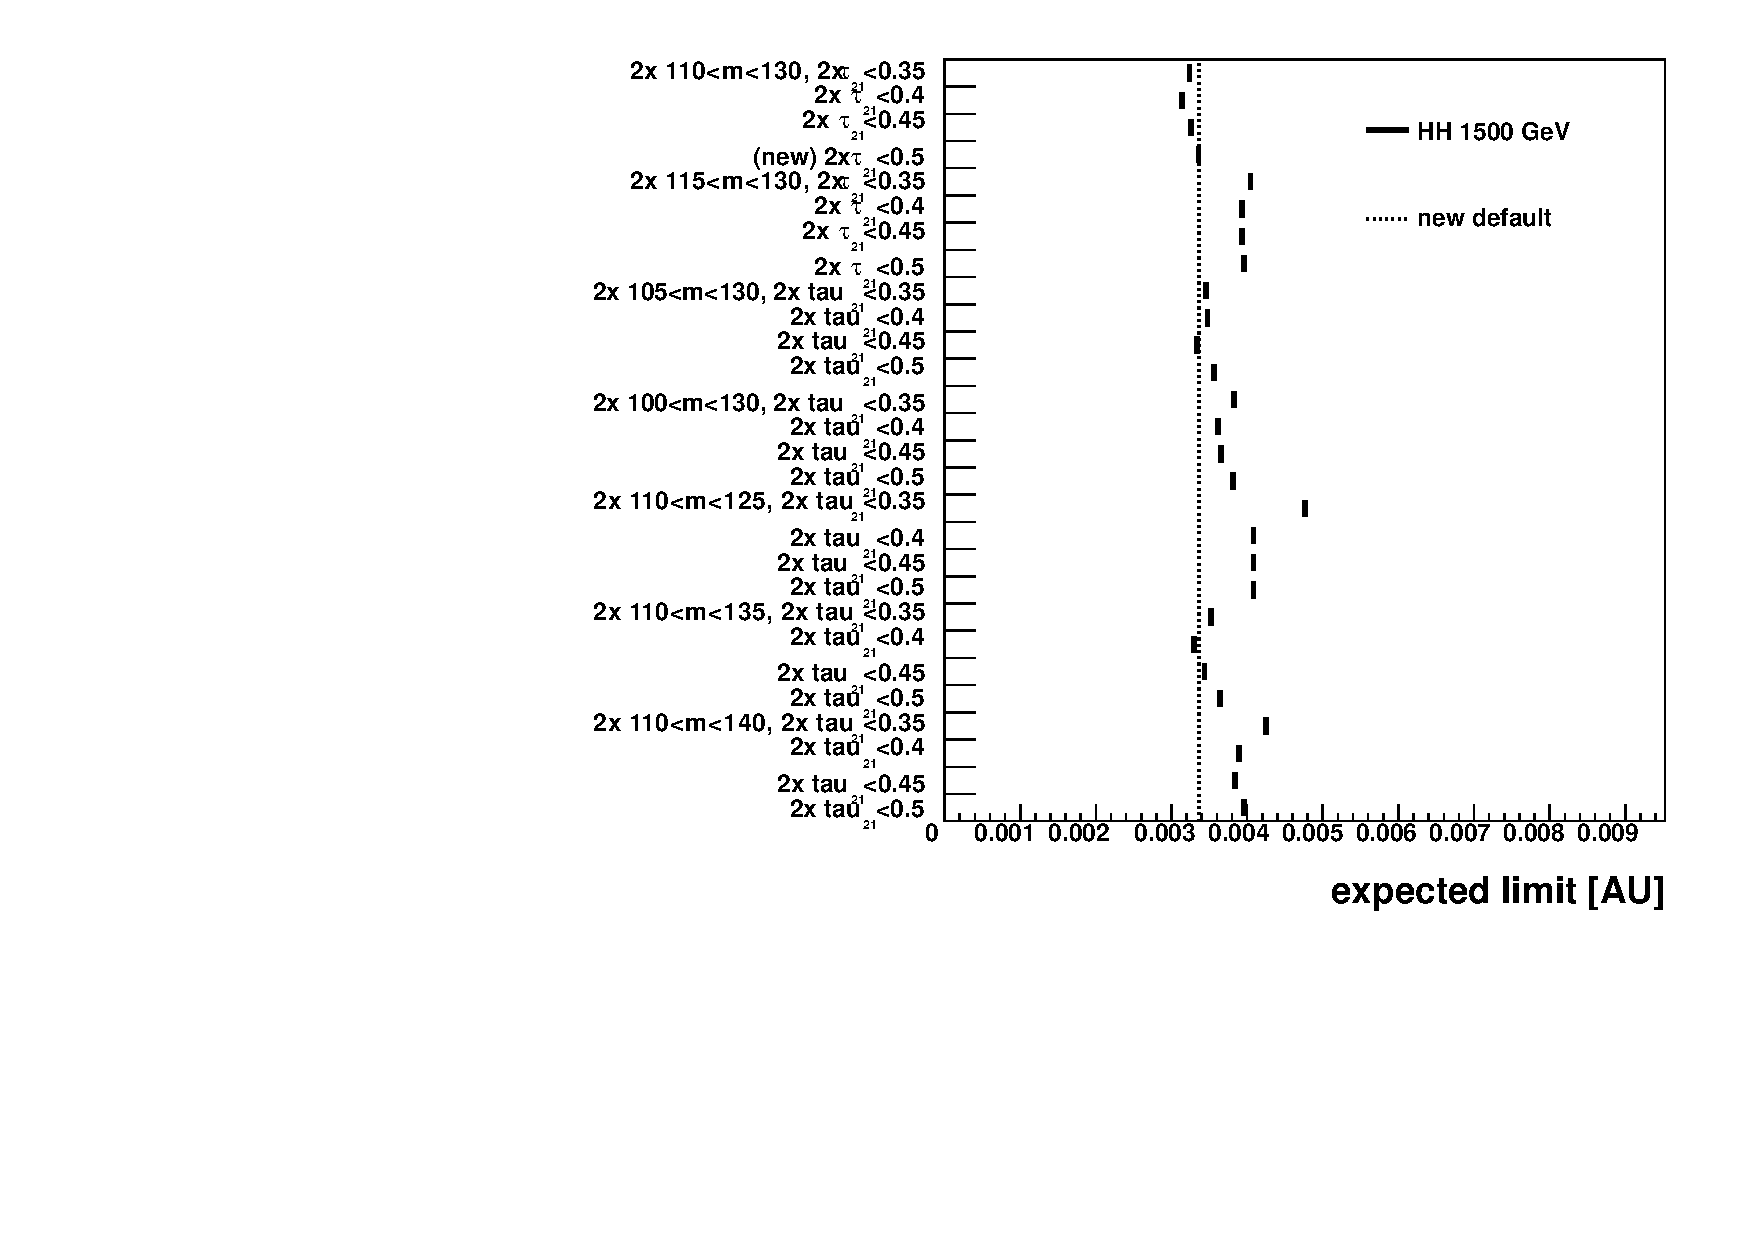
\includegraphics{figs/N-subjettiness/optimization1500_0.pdf}} &
     \resizebox{0.5\linewidth}{!}{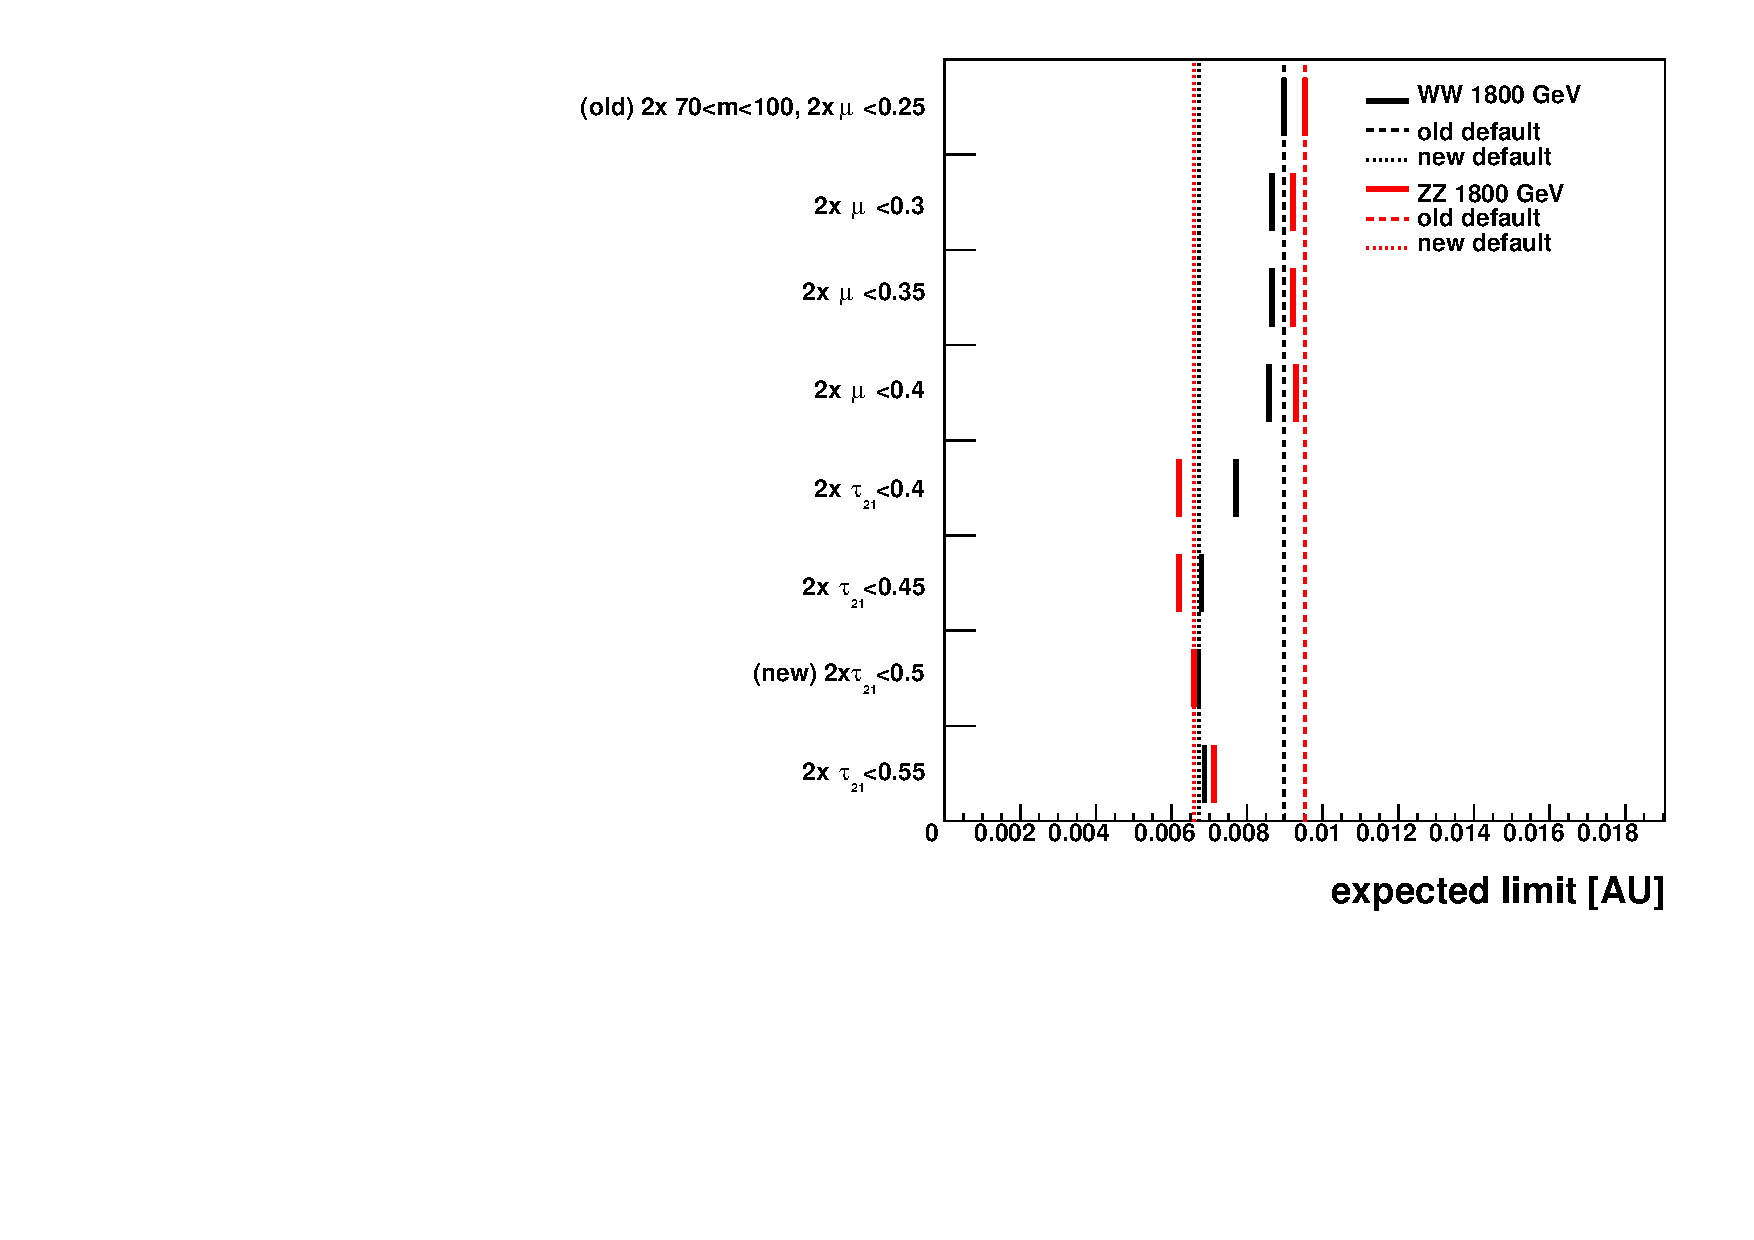
\includegraphics{EXO-12-024/figs/N-subjettiness/optimization1800_0.pdf}} \\
\end{tabular}
\caption[N-subjettiness]{Optimizataion of the N-subjettiness ($\tau_{21}$) or massdrop ($\mu$) cut value for the best expected limit.}
\label{fig:optimization0}
\end{figure}

Figure~\ref{fig:optimization1} shows the optimization of the pruned jet mass window cut.
Neither widing nor narrowing the pruned jet mass window on either side can improve the expected limit for WW and ZZ at the same time.
The jet mass window of $70 < m_\text{jet} <  100$~GeV provides best performance for WW and ZZ at the same time.

\begin{figure}[htb]
\centering
\begin{tabular}{cc}
     \resizebox{0.5\linewidth}{!}{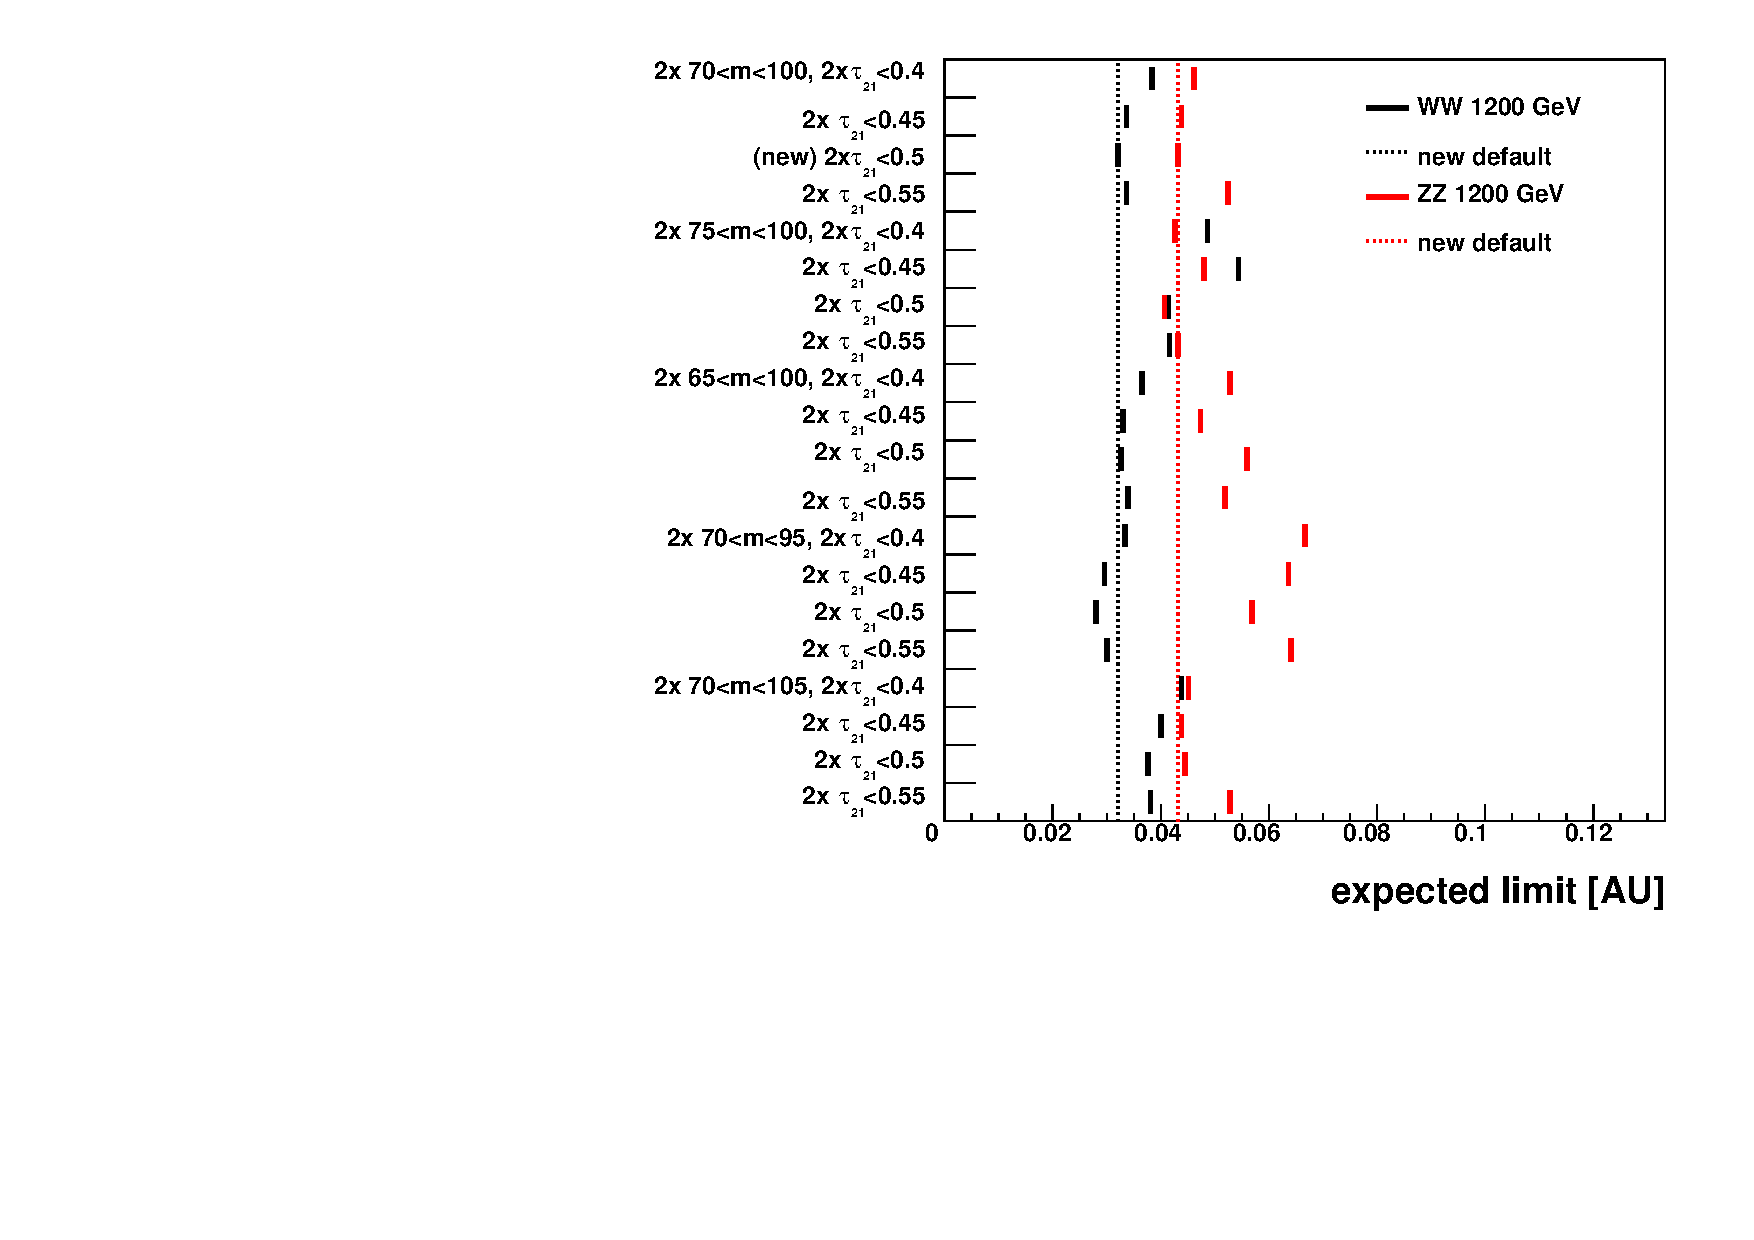
\includegraphics{EXO-12-024/figs/N-subjettiness/optimization1200_1.pdf}} &
%     \resizebox{0.5\linewidth}{!}{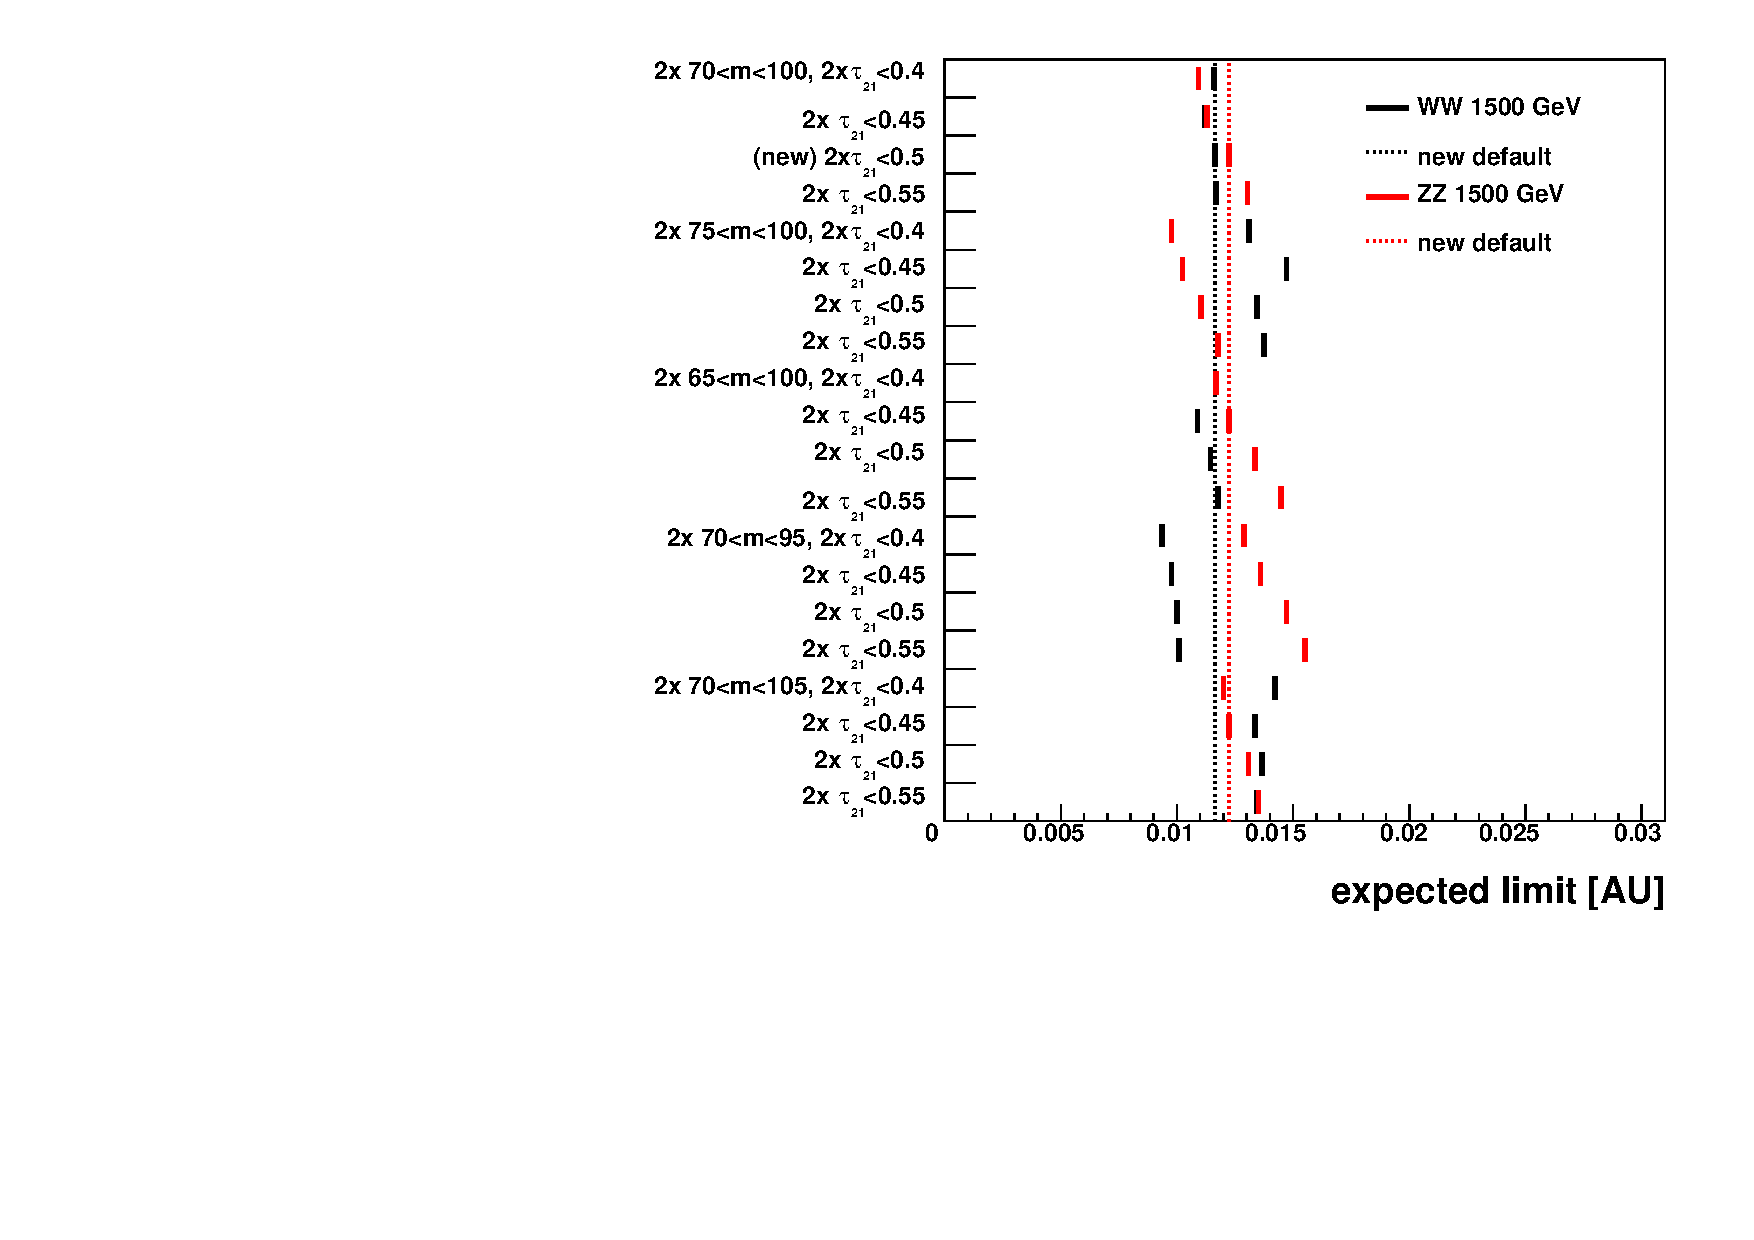
\includegraphics{figs/N-subjettiness/optimization1500_1.pdf}} &
     \resizebox{0.5\linewidth}{!}{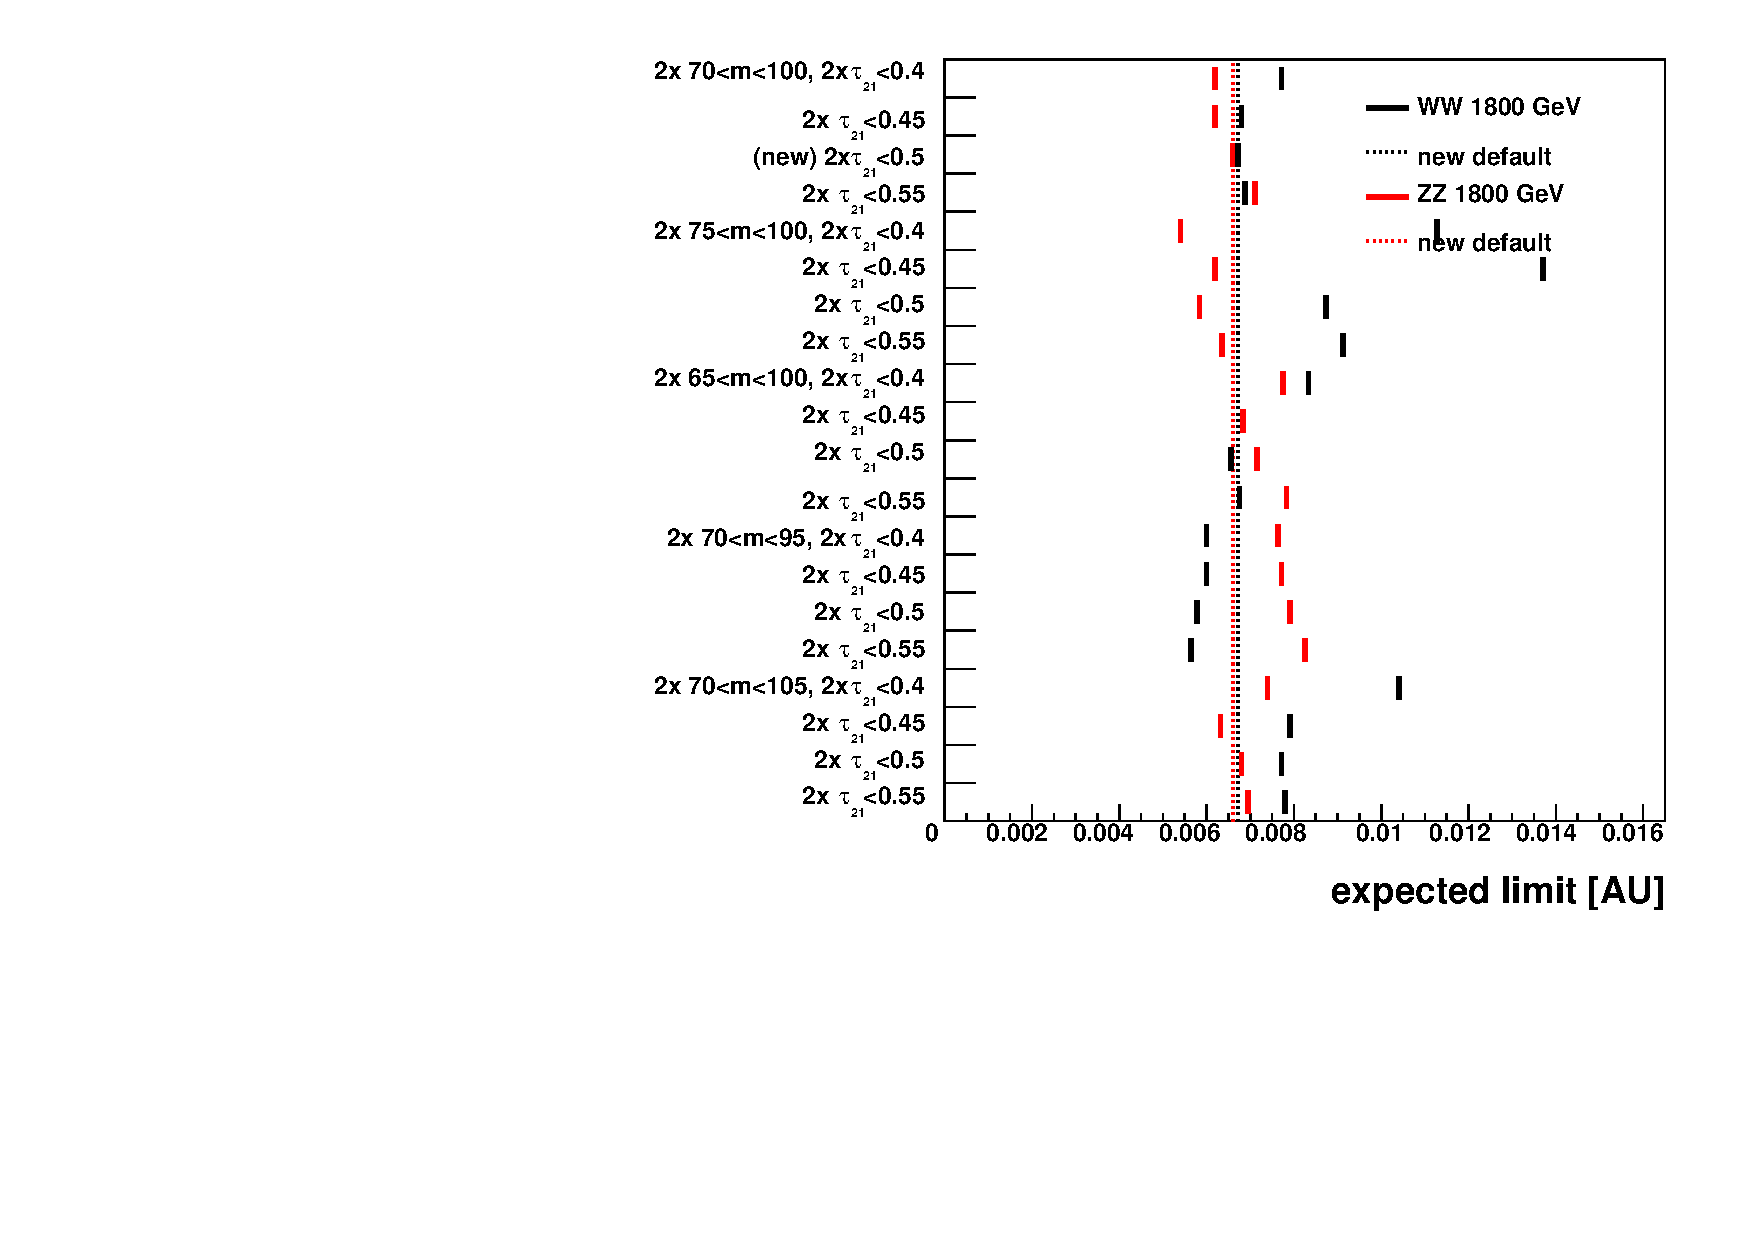
\includegraphics{EXO-12-024/figs/N-subjettiness/optimization1800_1.pdf}} \\
\end{tabular}
\caption[N-subjettiness]{Optimizataion of the pruned jet mass window cut for the best expected limit.}
\label{fig:optimization1}
\end{figure}

Figure~\ref{fig:optimization2} shows the dependency of the expected limit on the jet algorithm used for the resonance mass reconstruction.
It is found that AK5, AK7 and CA8 show almost the same performance.
This analysis switched since 2011 from AK5 to CA8 for consistency with other similar analyses. 
%EXO-12-021 and EXO-12-022.

\begin{figure}[htb]
\centering
\begin{tabular}{cc}
%     \resizebox{0.5\linewidth}{!}{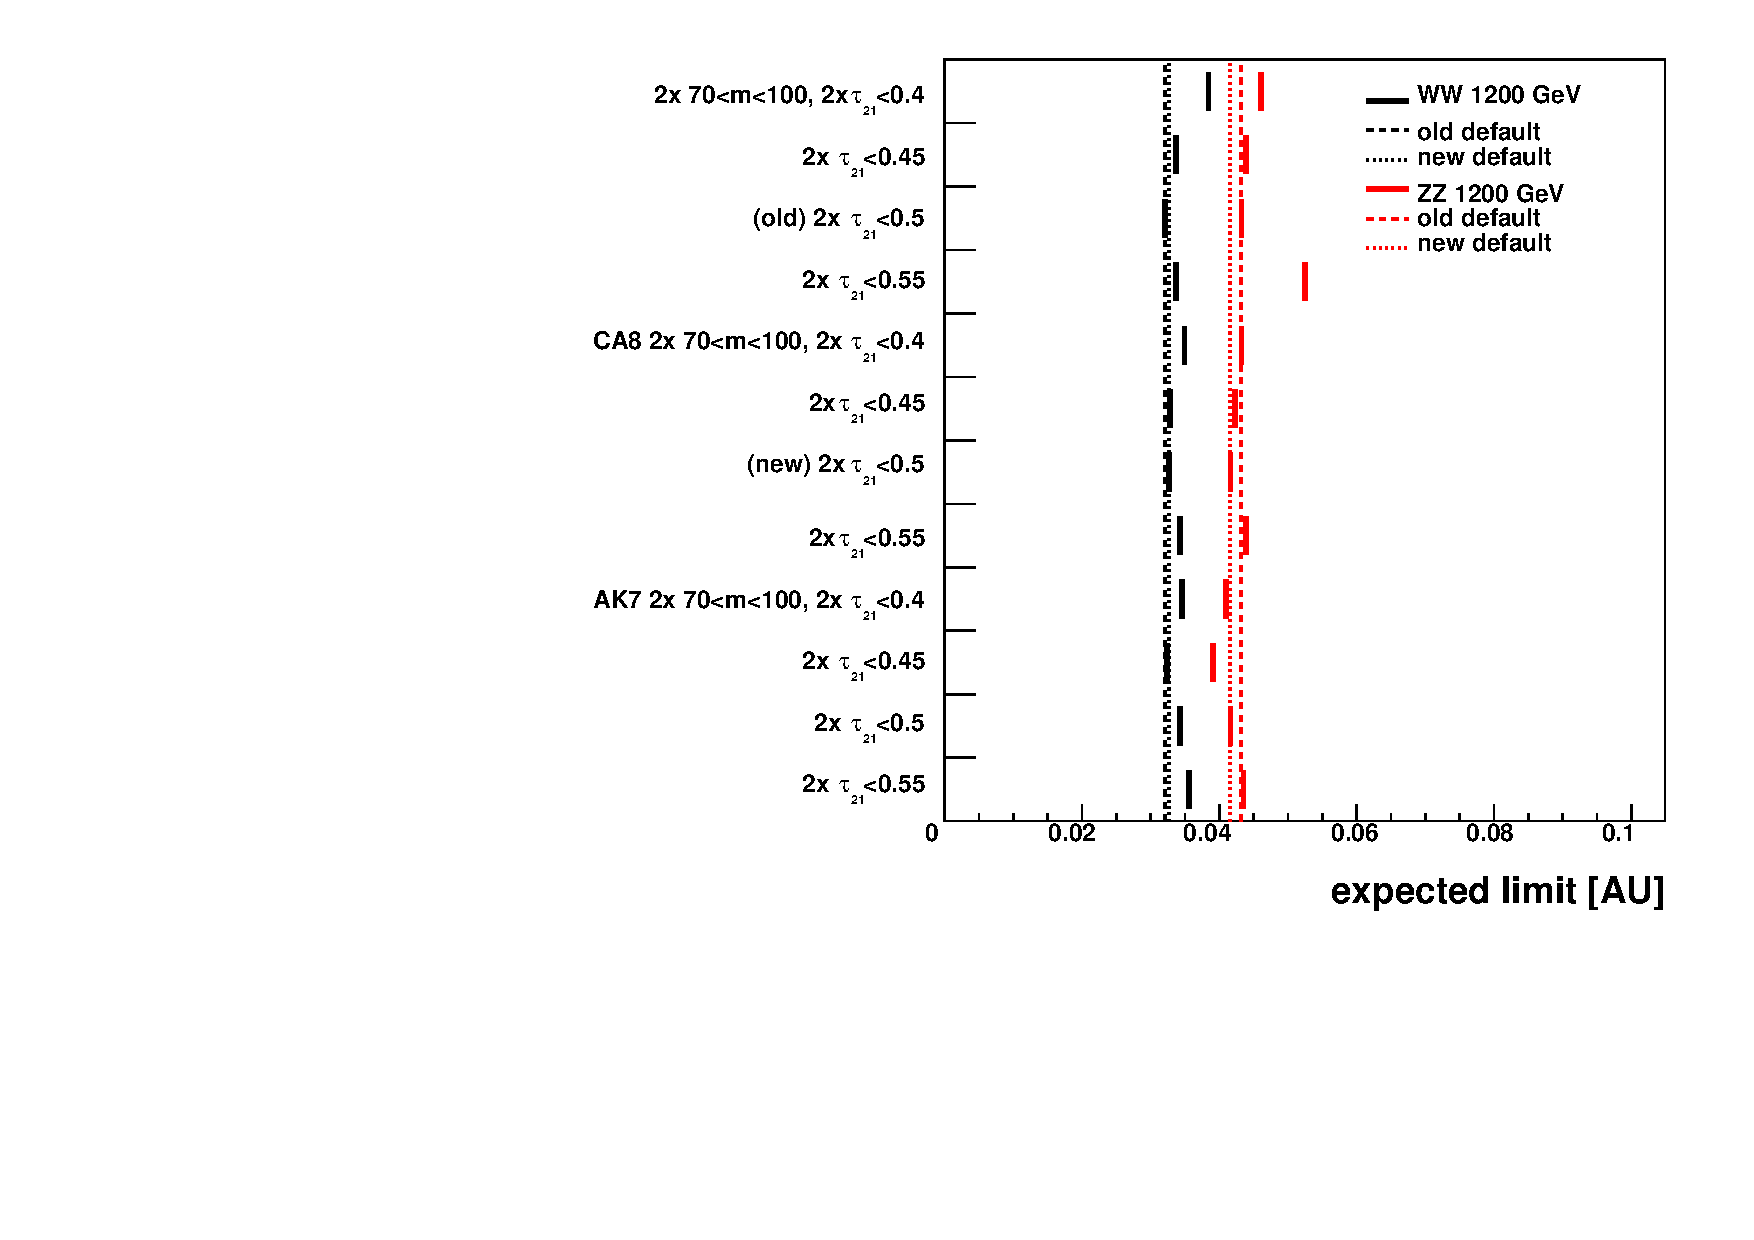
\includegraphics{figs/N-subjettiness/optimization1200_2.pdf}} &
%     \resizebox{0.5\linewidth}{!}{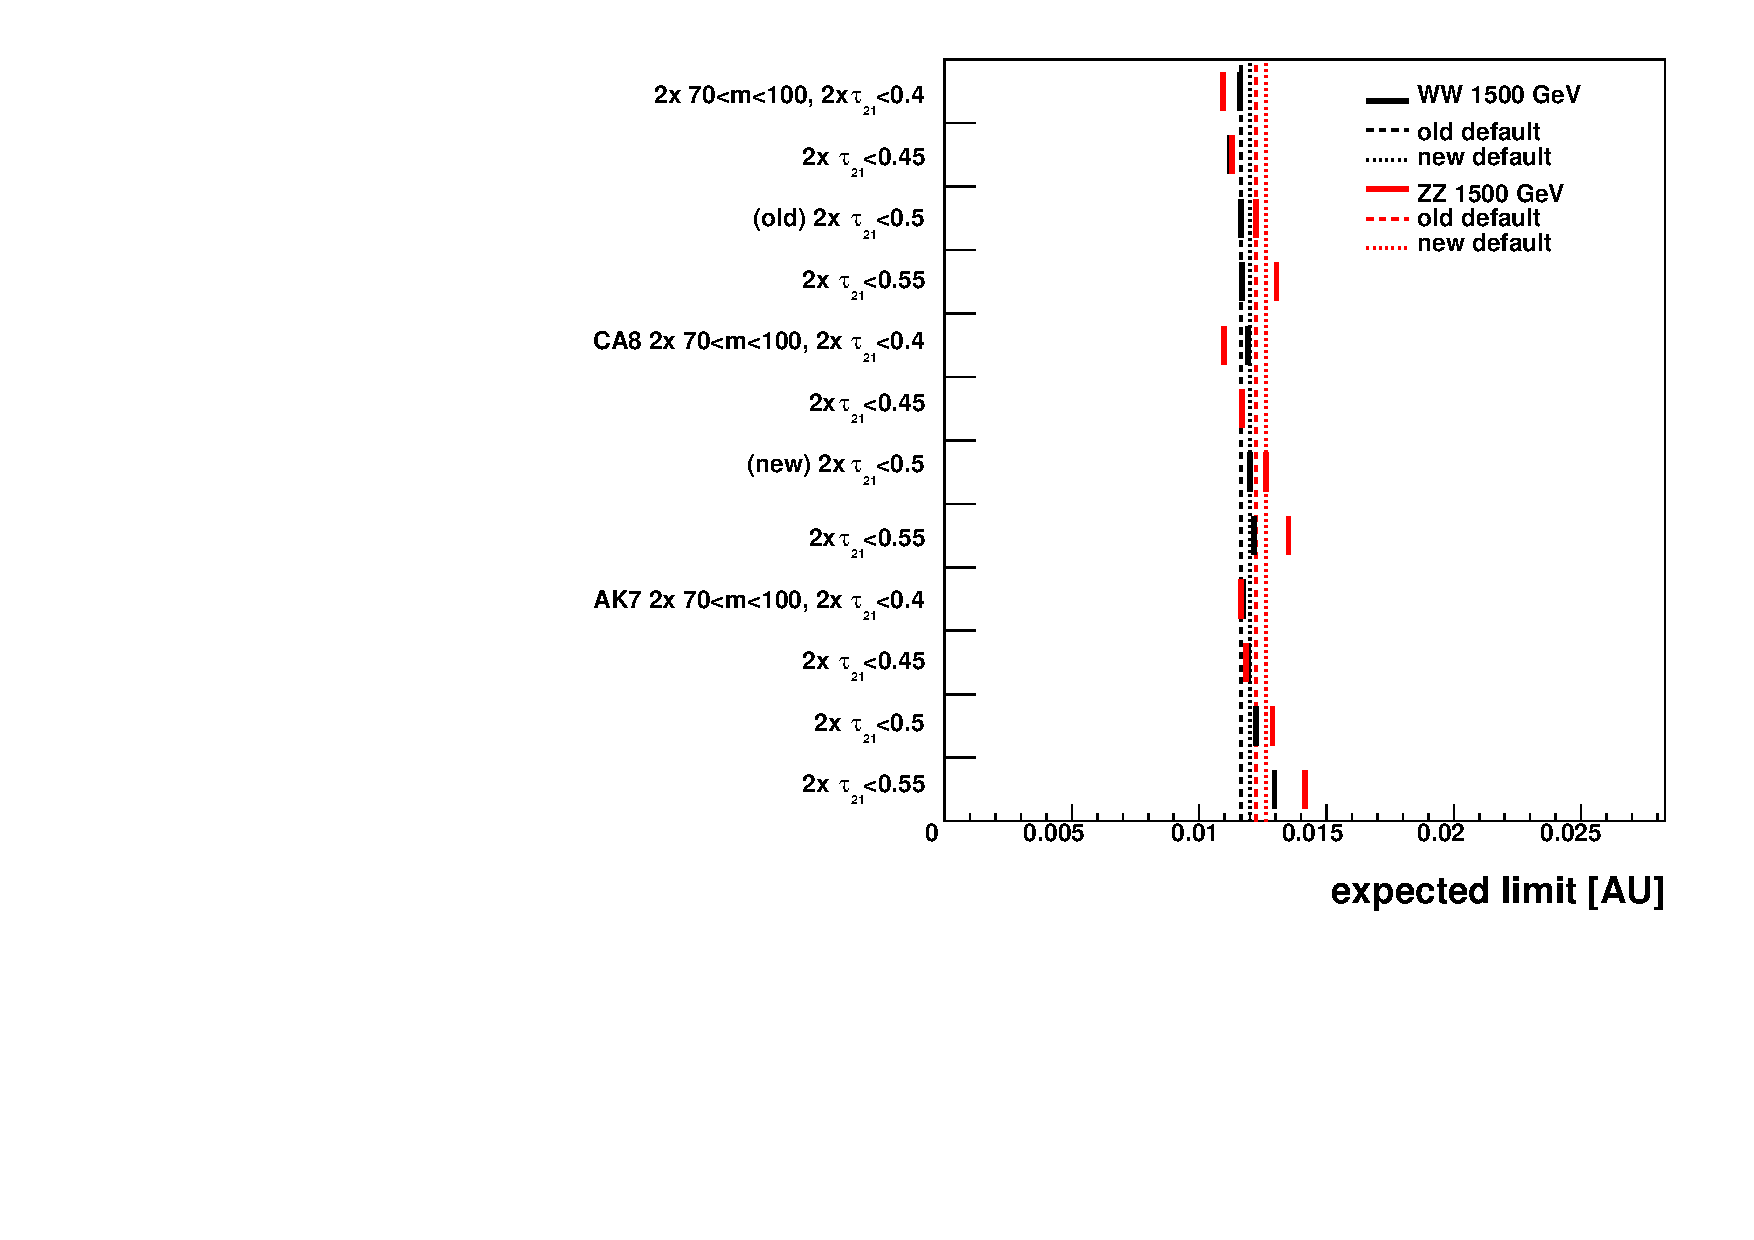
\includegraphics{figs/N-subjettiness/optimization1500_2.pdf}} &
     \resizebox{0.5\linewidth}{!}{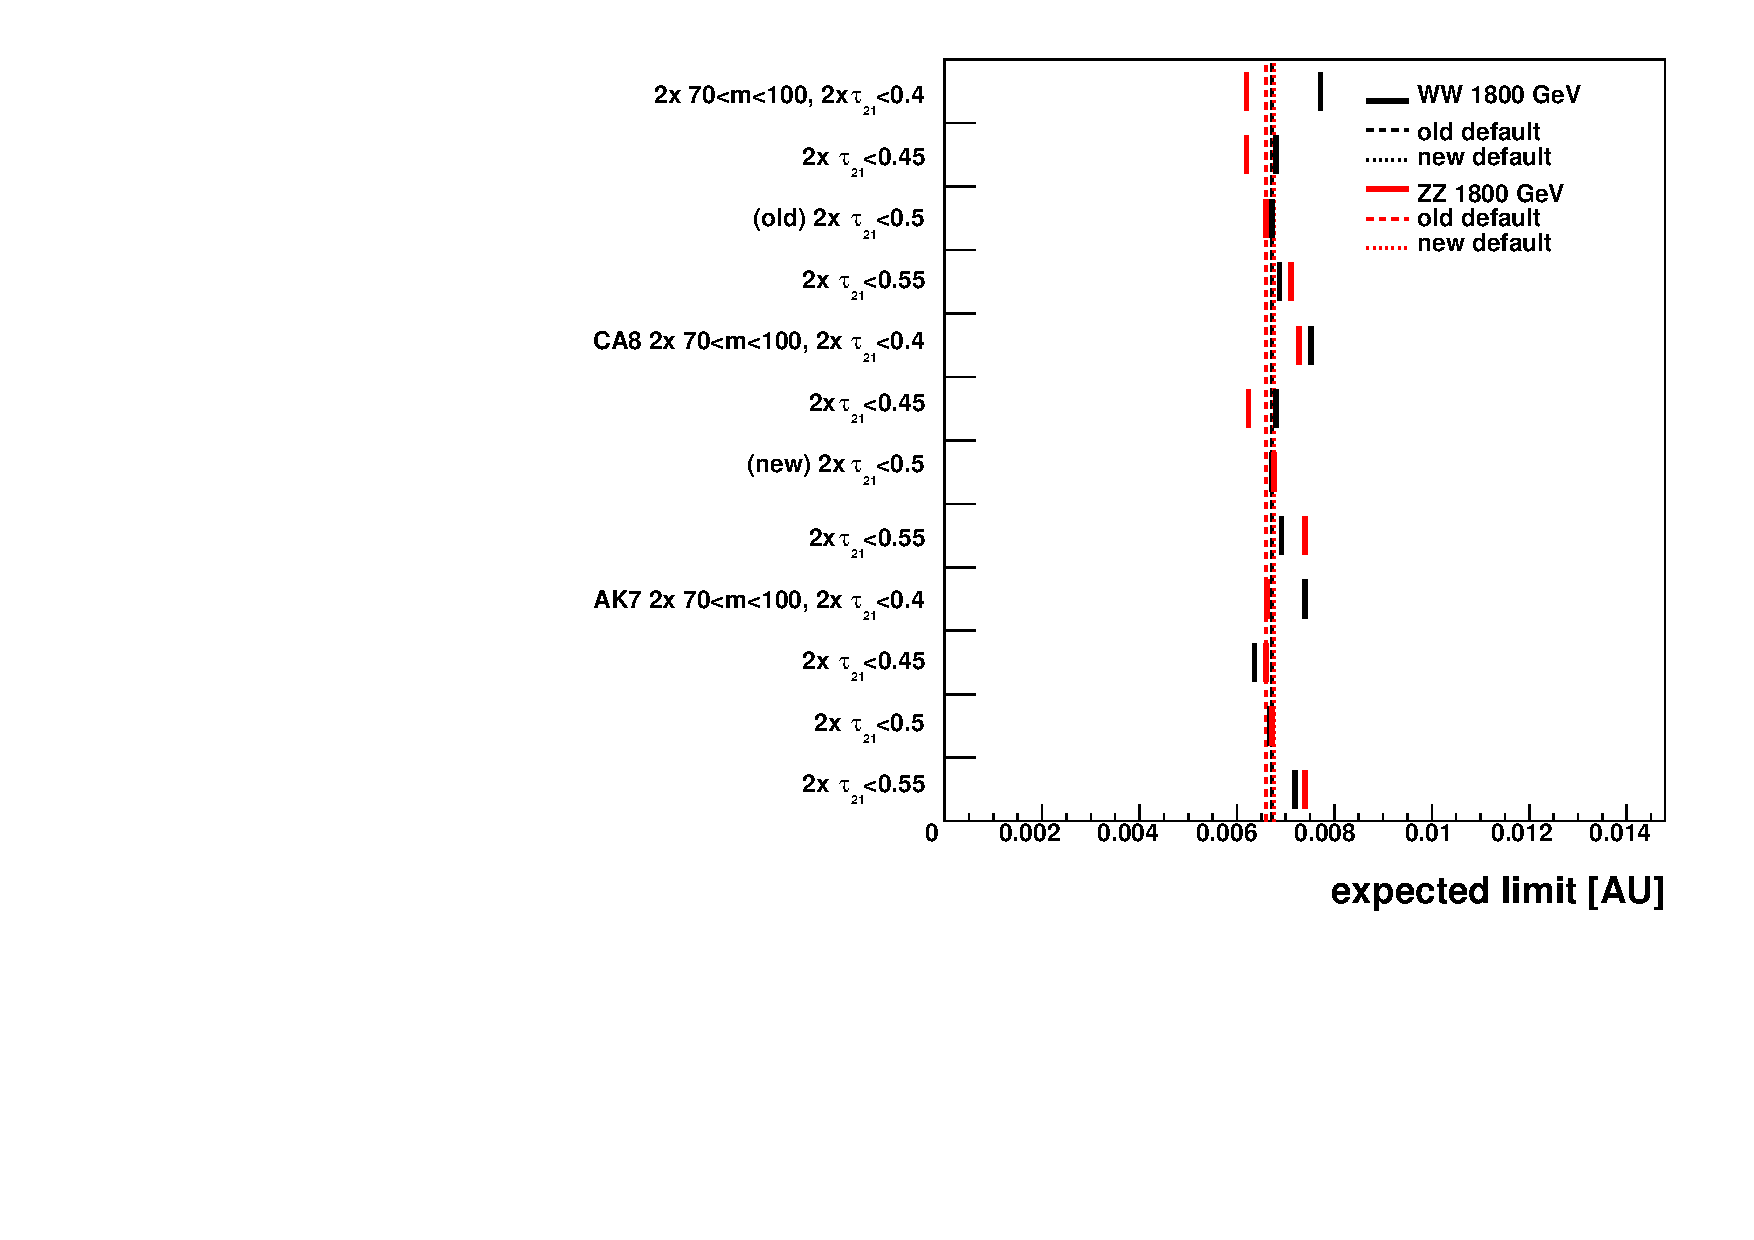
\includegraphics{EXO-12-024/figs/N-subjettiness/optimization1800_2.pdf}} \\
\end{tabular}
\caption[N-subjettiness]{Comparison of expected limit for different jet algorithms.}
\label{fig:optimization2}
\end{figure}

\section{The H tagging and W/Z tagging algorithms}
\label{sec: H tagging}

The products of hadronic decays of Higgs, W, and Z bosons can fall
within a single jet if these particles are highly boosted.  In this
analysis, we aim to cover as much of the Higgs branching ratio as
possible.  The Standard Model Higgs with a mass of 125 \GeVcc decays
to b$\bar{\rm b}$ with a branching fraction of 57.7\%, and to WW$^*$
with a braching fraction of 21.4\%.~\cite{pdg-higgs}.  Using these two
decay modes in a VH search, where WW$^*$ specifically decays to four
quarks, is the main topic of this note.  (The semileptonic decay mode
$ H \to WW \to 2q\ell \nu$ is viable, but its reconstruction is more
involved and will be covered in a subsequent analysis.)

%% &&& {\bf TO-DO: consider adding the branching fraction plot here. }


The algorithms to identify W/Z, ${\rm H \to b\bar{b}}$ and 
${\rm H \to WW^*}$ jets are necessarily different, but they use similar
jet-level variables: N-subjettiness (described in
Section~\ref{sec:N-subjettiness}) and jet pruning
(Section~\ref{sec:jetPruning}).  The W/Z-tagger is described in
Section~\ref{sec:wztagging}, and the two H-taggers in
Sections~\ref{sec:higgsTaggerbb} and ~\ref{sec:higgsTaggerww}.


%{\bf TO-DO: add a plot of this Higgs jet mass from signal, QCD, data, as a comparison.  And we need also to show the optimization of this mass choice. }

\subsection{N-subjettiness}
\label{sec:N-subjettiness}

N-subjettiness~\cite{Thaler:2010tr,Thaler:2011gf,Stewart:2010tn}
exploits the fact that the pattern of the hadronic decay of a heavy
object is reflected through the presence of distinctive energy lobes
corresponding to the decay products, as opposed to QCD jets which
present a more uniformly spread energy configuration. 
The inclusive jet shape N-subjettiness is
defined, in its generalized version~\cite{Thaler:2010tr}, as
%
\begin{equation}
\tau_N = \frac{1}{d_{0}} \sum_{k} p_{T,k}\,min( (\Delta R_{1,k})^{\beta}, (\Delta R_{2,k})^{\beta}...(\Delta R_{N,k})^{\beta})
\end{equation}
%
where the index $k$ runs over the jet constituents and the distances
$\Delta R_{n,k}$ are calculated with respect to the axis of the $n^{\mathrm{th}}$
subjet. The normalization factor $d_{0}$ is calculated as $d_{0}=
\sum_{k} p_{T,k}R^{\beta}_{0}$, setting $R_{0}$ to the jet radius of
the original jet. In the analysis, we use onepass\_kt\_axes definition
of subjet axes and the N-subjettiness is calculated
from the unpruned jets with the parameter $\beta=1$. 
It has been shown in the literature~\cite{Thaler:2010tr} that the
best way to separate (N+1)-prong from the N-prong decays merged into
a single jet is to select jets with low value of the ratio $\tau_{N+1}/\tau_N$.
In this vein, the variable able to best discriminate between $\PW/\cPZ$ jets and QCD jets
is $\tau_{21}=\tau_{2} / \tau_{1}$. The distribution of $\tau_{21}$ for
the VV signal and QCD background is given in Fig.~\ref{fig:N-sub-mass}.
%While, 
%the best variable to discriminate $H \to WW$ is $\tau_{42}=\tau_{4} / \tau_{2}$, given in 
%Fig.~\ref{fig:tau421TeV} and Fig.~\ref{fig:tau422TeV}.

\begin{figure}[htb]
\centering
\begin{tabular}{cc}
     \resizebox{0.5\linewidth}{!}{\includegraphics{figs/N-subjettiness/Signal_MC_Pre.pdf}} &
     \resizebox{0.5\linewidth}{!}{\includegraphics{figs/N-subjettiness/Signal_MC.pdf}} \\
\end{tabular}
\caption[N-subjettiness]{Comparison for $\tau_{2}/\tau_{1}$ distribution 
between signal (red) and background (black) 
before the jet mass cut (left) and after 
the jet mass cut of [70, 100]~GeV applied (right). 
The signal MC used here is Herwig WW 1.5 TeV, and background is Herwig QCD.}
\label{fig:N-sub-mass}
\end{figure}

%\textbf{PLAN} in Fig~\ref{N-sub} and Fig~\ref{N-sub-mass}, I'm gonna add prettier plots for different signals(pythia and herwig, 1.0Tev to 3.0TeV resonance).  

%The leading two ungroomed CA8 jets to the leading two pruned CA8 jets are matched requireing $\Delta R < 0.5 $, which fails in less than 0.1\% of the events.




\subsection{Jet Pruning}
\label{sec:jetPruning}

Jet pruning consists of the removal of the softest
components of the jets~\cite{catop_cms,topwtag_pas}.
The jet pruning algorithm uses the CA $R=0.8$ jets as inputs. In the
process, soft and wide-angle particles (relative to the parent in the
clustering) are ignored and are not clustered.  
The same parameters are chosen for the jet
pruning algorithm as in the original paper~\cite{jetpruning1,jetpruning2}.

%% &&& from Petar: is this really true?  I thought that the pruning
%% &&& reruns the CA8 jet clustering from scratch, but in the process
%% &&& prunes the soft and wide-angle PF candidates from the jet.
%% &&& We should check this...


The result of jet pruning on the CA8 jets is two fold, i.e., the invariant jet mass 
reconstruction and subjet indentification.
In all cases,
we use the jet invariant mass computed from the whole (or ``fat'') 
pruned jet.  This quantity is referred below to as the pruned jet mass.
For W/Z tagging, we use pruned jet mass between 70 and 100 \GeVcc. 
%is sychorinzed with VV search~\cite{EXO-12-024}.
For the identification of Higgs jets, we require the pruned jet mass to
lie between 110 and 135~\GeVcc.  The distribution of the pruned jet
mass of the Higgs candidate jet is shown on Fig.~\ref{fig:JetMassTagging} 


\begin{figure}[htb]
\begin{center}
%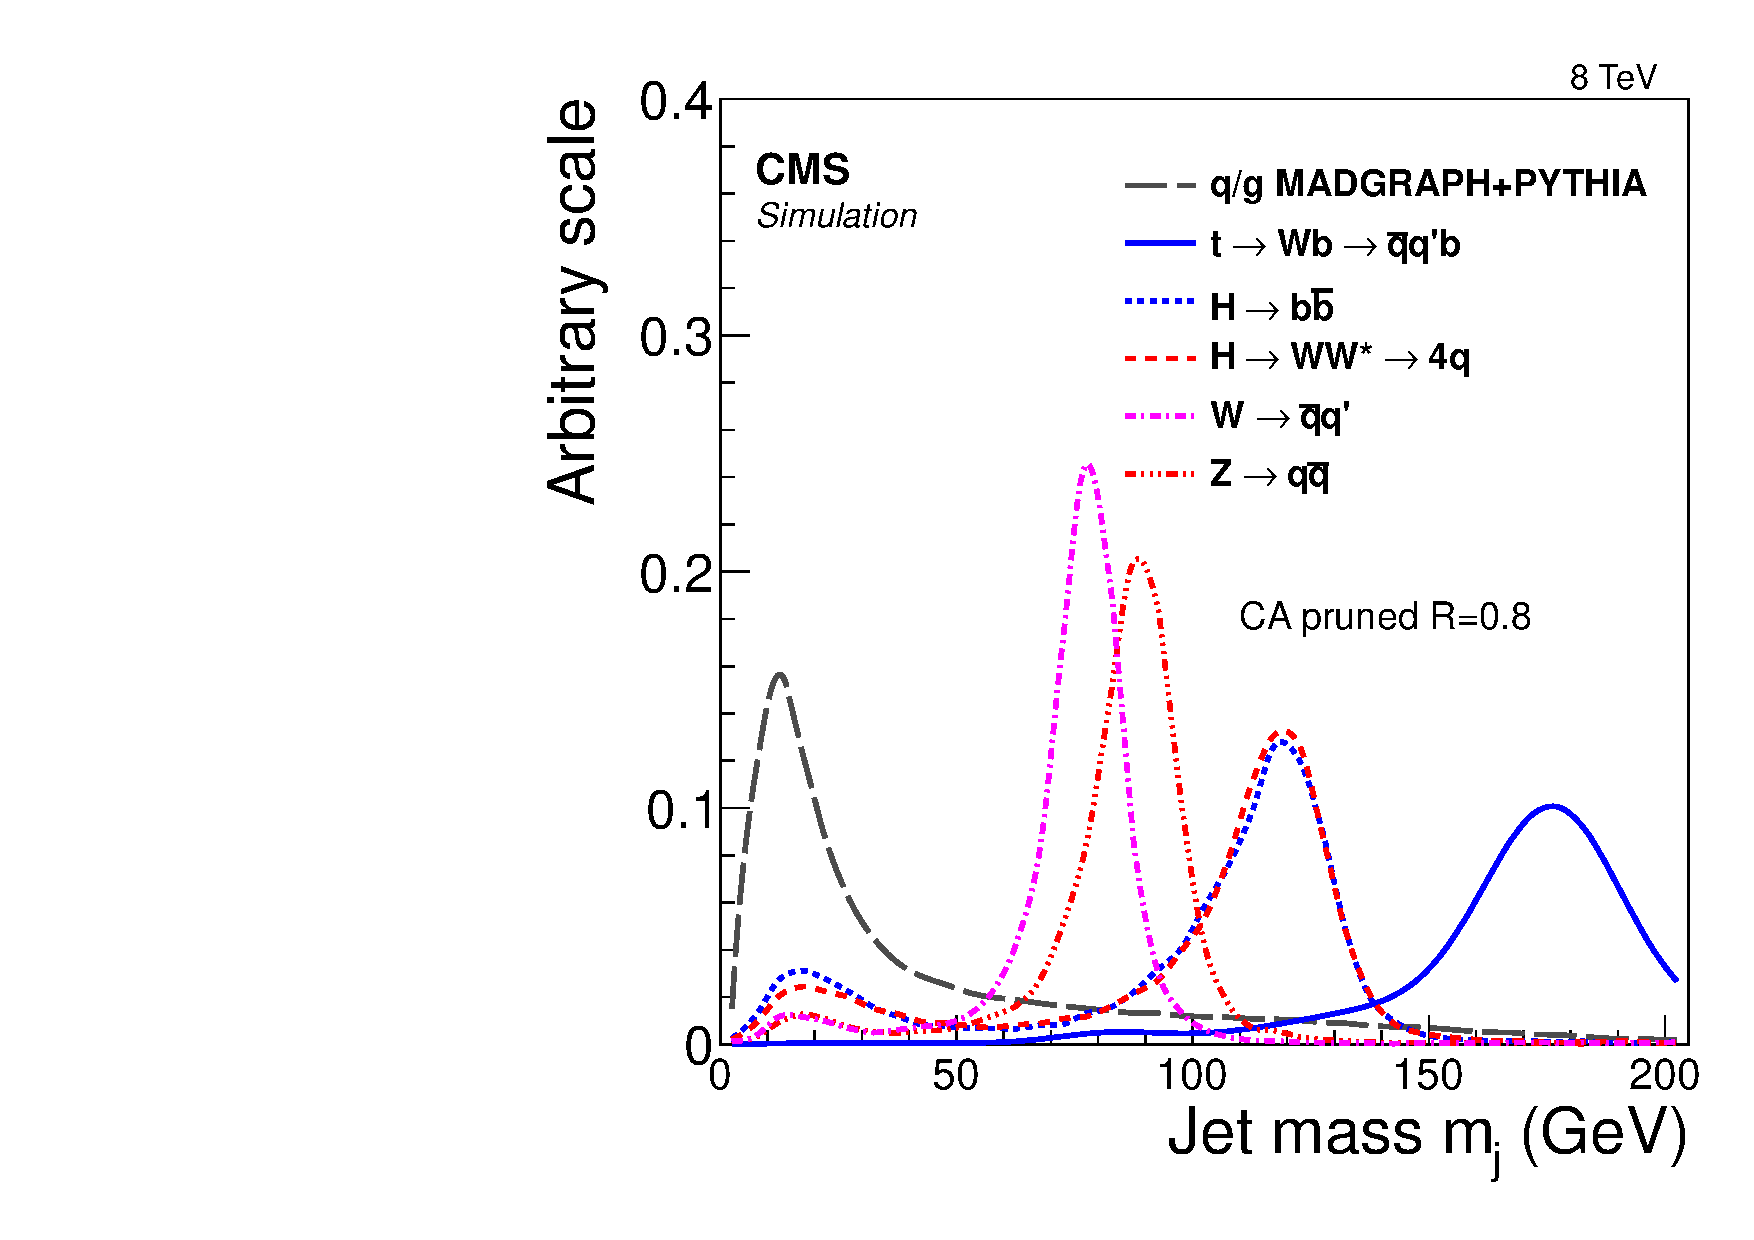
\includegraphics[width=0.49\textwidth]{HbbZqqfigs/Signal/signal-data-qcd-jetmass.pdf}
%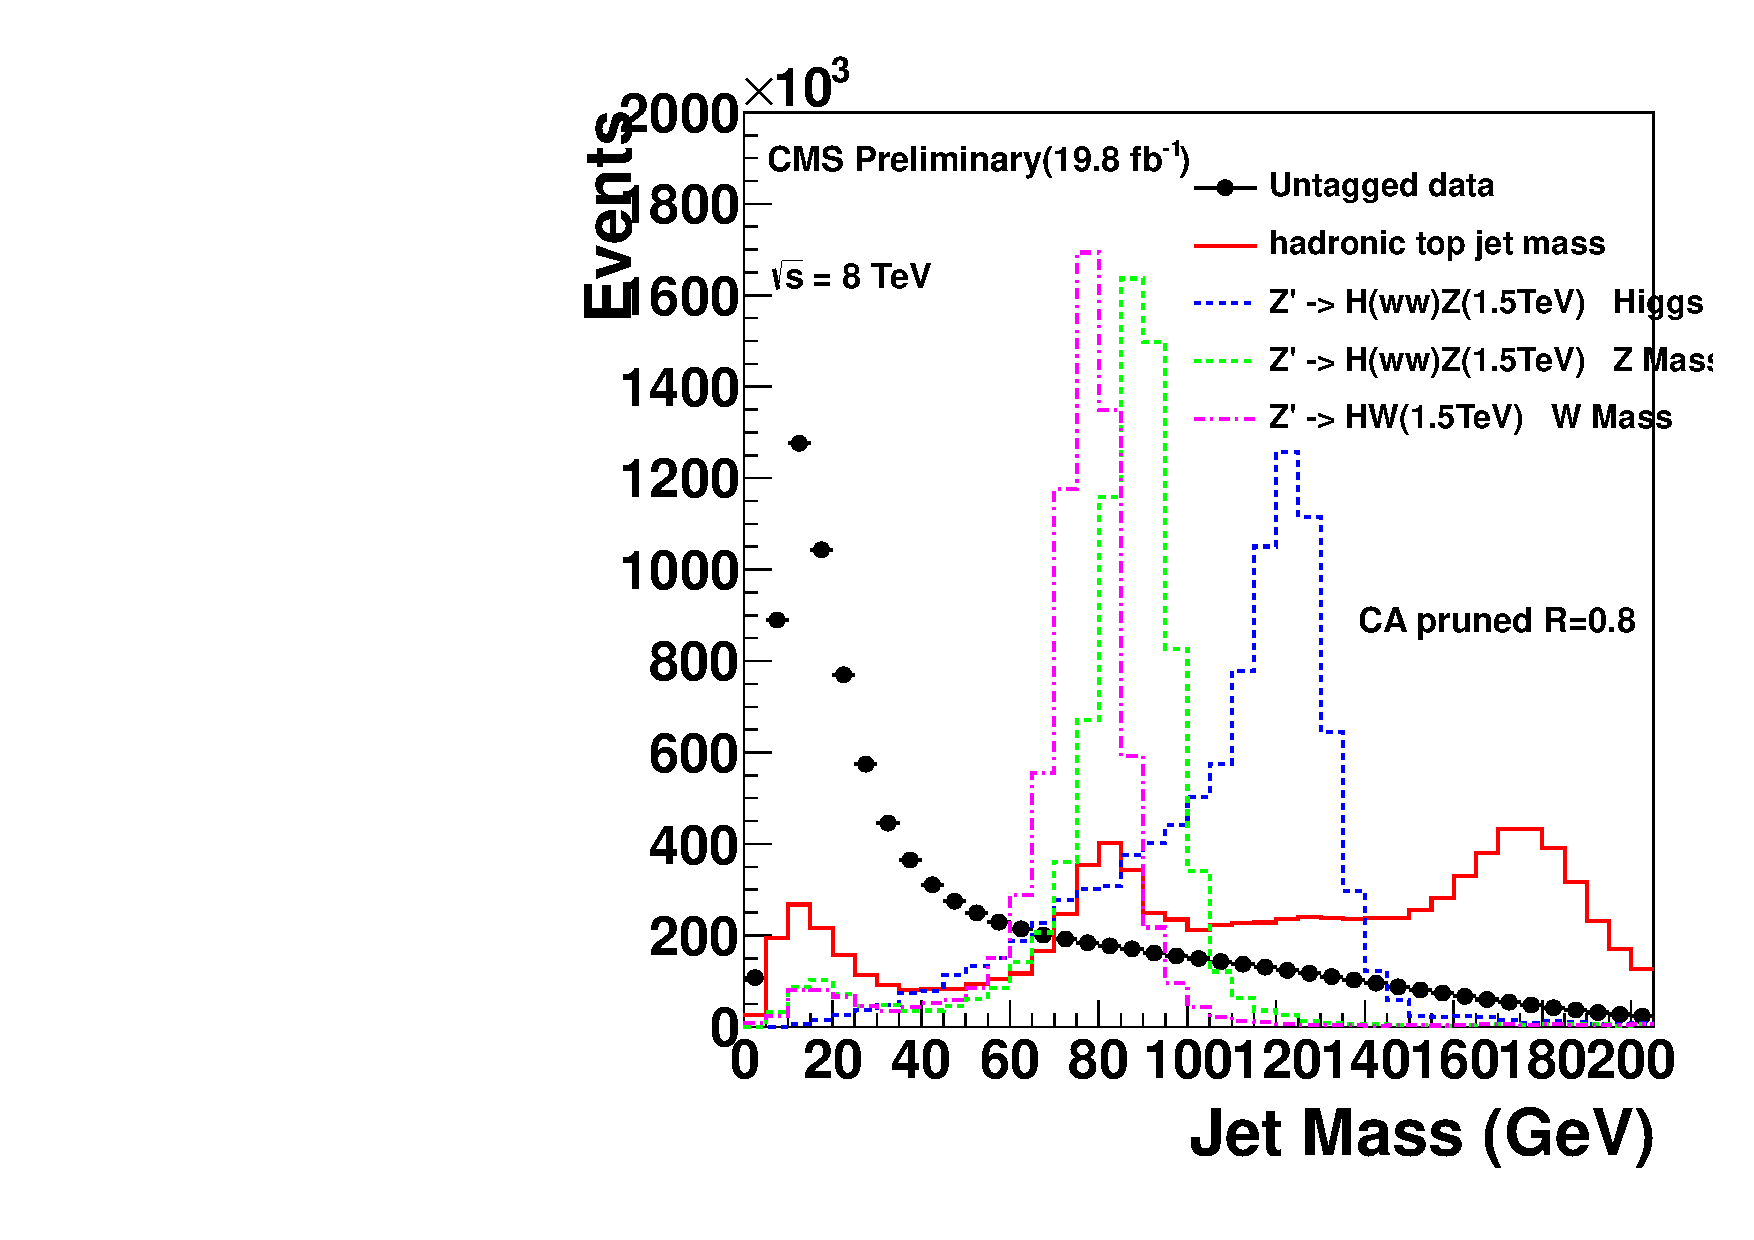
\includegraphics[width=0.49\textwidth]{HqqqqZqqfigs/Signal/signal-data-qcd-jetmass.pdf}
%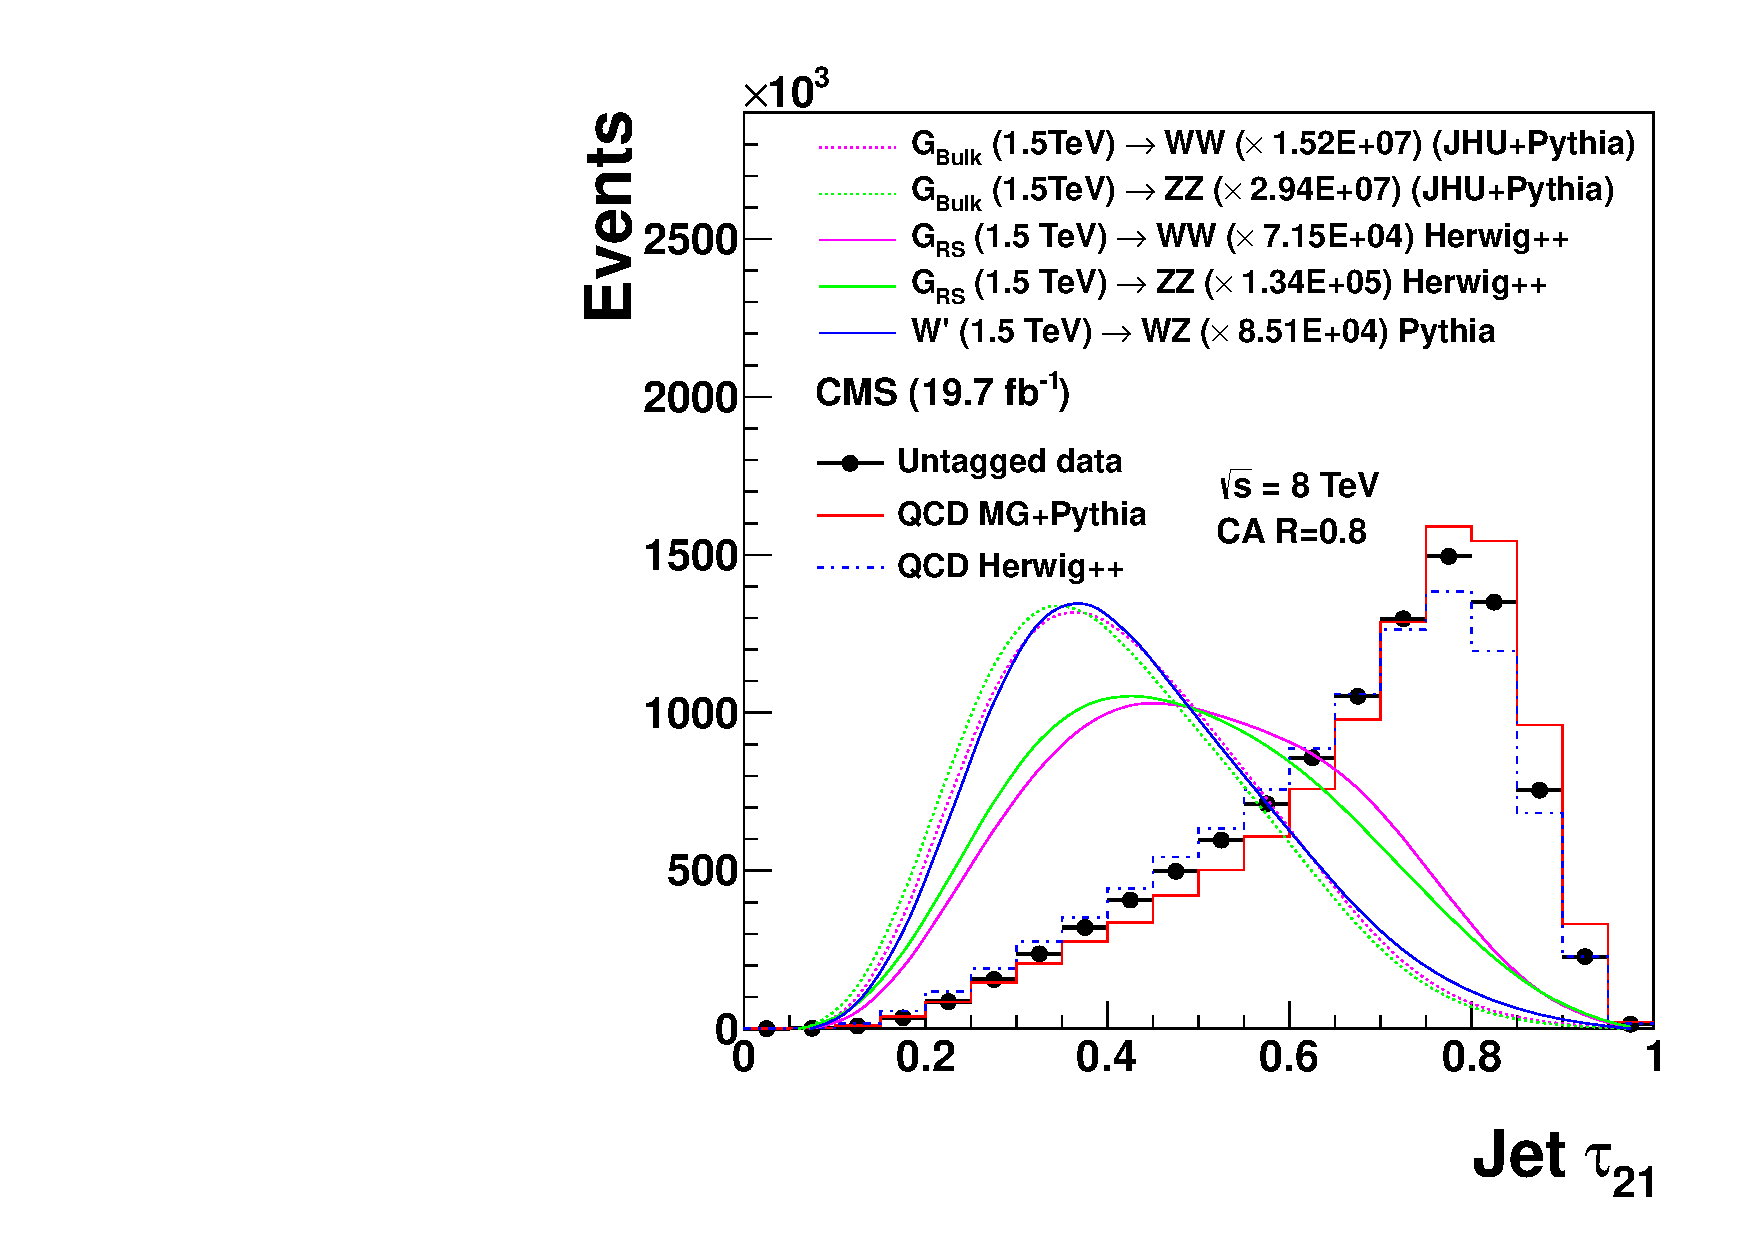
\includegraphics[width=0.49\textwidth]{figs/signal-acc-eff/signal-data-qcd-Jet-Tau21.pdf}
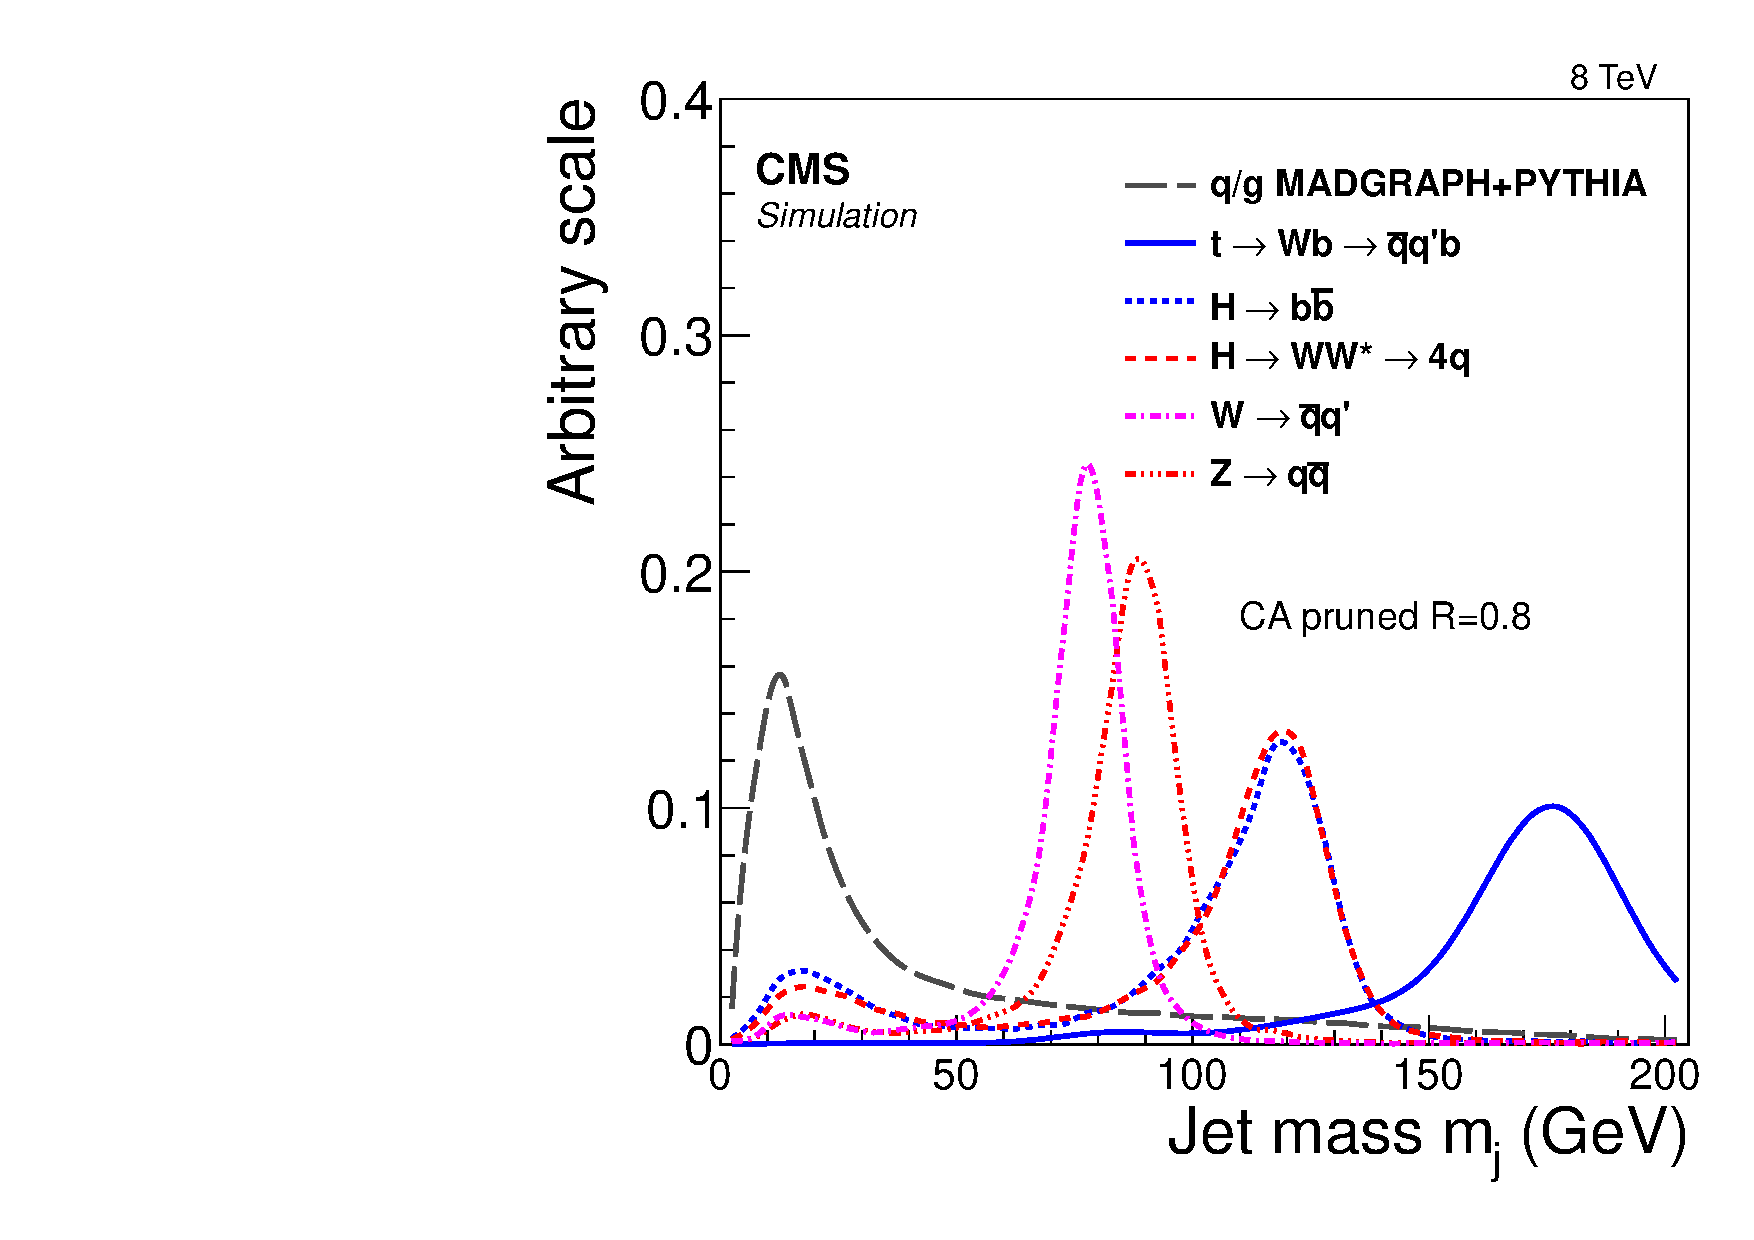
\includegraphics[width=0.69\textwidth]{HbbZqqfigs/Signal/signal-data-qcd-jetmass.pdf}
\end{center}
\caption{Pruned jet mass in signal MC, data and $t\overline{t}$ MC. 
  MC samples are normalized to data.  MC
  distributions are plotted as smooth curves connecting the histogram
  entries; the MC histograms have the same binning as the data.
  Higgs, W/Z and top jets are matched to their generator level particles, 
  respectively. }
%The pruned jet mass of $\Hbb$ jets is shown on
%  the left, and of $\Hww$ jets on the right.}
%  MC is normalized to fit into the plot.  }
 % The signal MC
 % distributions are plotted as smooth curves connecting the histogram
  %entries. 
\label{fig:JetMassTagging}
\end{figure}


The main role of jet pruning is to allow better delineation of subjets
within the jet.  In ${\rm H \to b\bar{b}}$ tagger, the axes of the 
pruned subjets are used as the basis for b tagging.



\subsection{W/Z tagging  } 
\label{sec:wztagging}

For the identification of W/Z jets, we employ the same tagging algorithm 
previously used in published 
searches~\cite{CMS:2013fea}.  W/Z jets are selected using the following
requirements:
\begin{itemize}

\item {\bf Pruned jet mass}  $\mbox{\boldmath$m_{\text{jet}}$}$
  - Require the total pruned jet mass to satisfy $70 \GeVcc < m_\text{jet} <  100 \GeVcc $.

\item {\bf N-subjettiness} 
  - We split the events into two categories, ``high purity'' $\PW/\cPZ$ jets by
    requiring $\tau_{21} \leq 0.5$, while $ 0.5 < \tau_{21} < 0.75$ defines 
    the ``low purity'' $\PW/\cPZ$ jets.  The thresholds are taken from the published VV
    search.

\end{itemize}
The performance of the W/Z tagger has been documented in detail in Ref.~\cite{JME-13-006}.





%\subsection{Optimization of the Higgs Mass window }







%{\bf TO-DO: add a plot of this Higgs jet mass from signal, QCD, data, as a comparison. 
% Also show the optimization of the resulting choice of the mass window. }

%% &&& {\bf HH to 4b might explain this. }


\subsection{${\rm H \to b\bar{b}}$}
\label{sec:higgsTaggerbb}

To identify Higgs jets arising from the shower and hadronization of two 
collimated b quarks, we apply b tagging either on the two subjets or the
fat jet , based on the angular separation of the two subjets, which is 
recommended by BTV-13-001~\cite{BTV-13-001}. 
%CSV B tagging method on the jets, no matter subjets or fat jets, 
%uses a fixed cone size of 0.3 to collects the tracks around 
%the jet axis. 

 we use the following selection, syncrhonized with
the radion search to $\PH\PH \to {\rm 4b}$~\cite{HH4b} and the search for HW 
resonances in the semileptonic channel~\cite{HWlv}:
\begin{itemize}

\item {\bf Pruned jet mass}  $\mbox{\boldmath$m_{\text{jet}}$}$
  - Require the total pruned jet mass to satisfy $110 \GeVcc < m_\text{jet} <  135 \GeVcc $.

\item {\bf Subjet b-tagging}
        \begin{itemize}
	\item if $\Delta R$ between the CA8 subjets is bigger than 0.3: 
  		{\it both} subjets must pass the CSV Loose working point.
	\item if $\Delta R$ between the CA8 subjets is smaller than 0.3:
		require the {\it fat} CA8 jet to pass the CSV Loose working point. 
        \end{itemize}

\end{itemize}



\subsection{${\rm H \to WW^* \to 4q}$}
\label{sec:higgsTaggerww}

%tau4/tau2 < 0.5

In this channel, Higgs decays to two W bosons, one real and one
virtual (denoted with an asterisk).  Given that this is effectively a
three-body decay ${\rm H\to Wqq}$, the jets from the four quarks are
not on an even footing -- the subjets from the real W are harder, and
they also form a W mass.  The subjets from the softer two quarks are
less well defined.

A naive ${\rm H \to 4q}$ tagger would require a fat jet with four subjets. 
%{\bf TO-DO: add the plot with the number of subjets.}
However, a study done using the subjets as defined by the CMS Top Tagging
algorithm (which reruns the CA8 jet clustering with additional weak 
pruning~\cite{cmstoptagging}) removes $\approx 90\%$ of the signal.   
Compounded with a decreasing angular separation
between Higgs decay products, 
 as a function of the Higgs \pt, at higher 
resonance masses, {\it e.g.} at 2\TeVcc, only 1\% of signal 
passes this selection. 
The distribution of the number of subjets of the reconstructed Higgs jets 
in signal MC (obtained from the CMS Top Tagging) is shown 
in Fig.~\ref{fig:Nsubjets}

\begin{figure}[htb]
\centering
\begin{tabular}{cc}
     \resizebox{0.7\linewidth}{!}{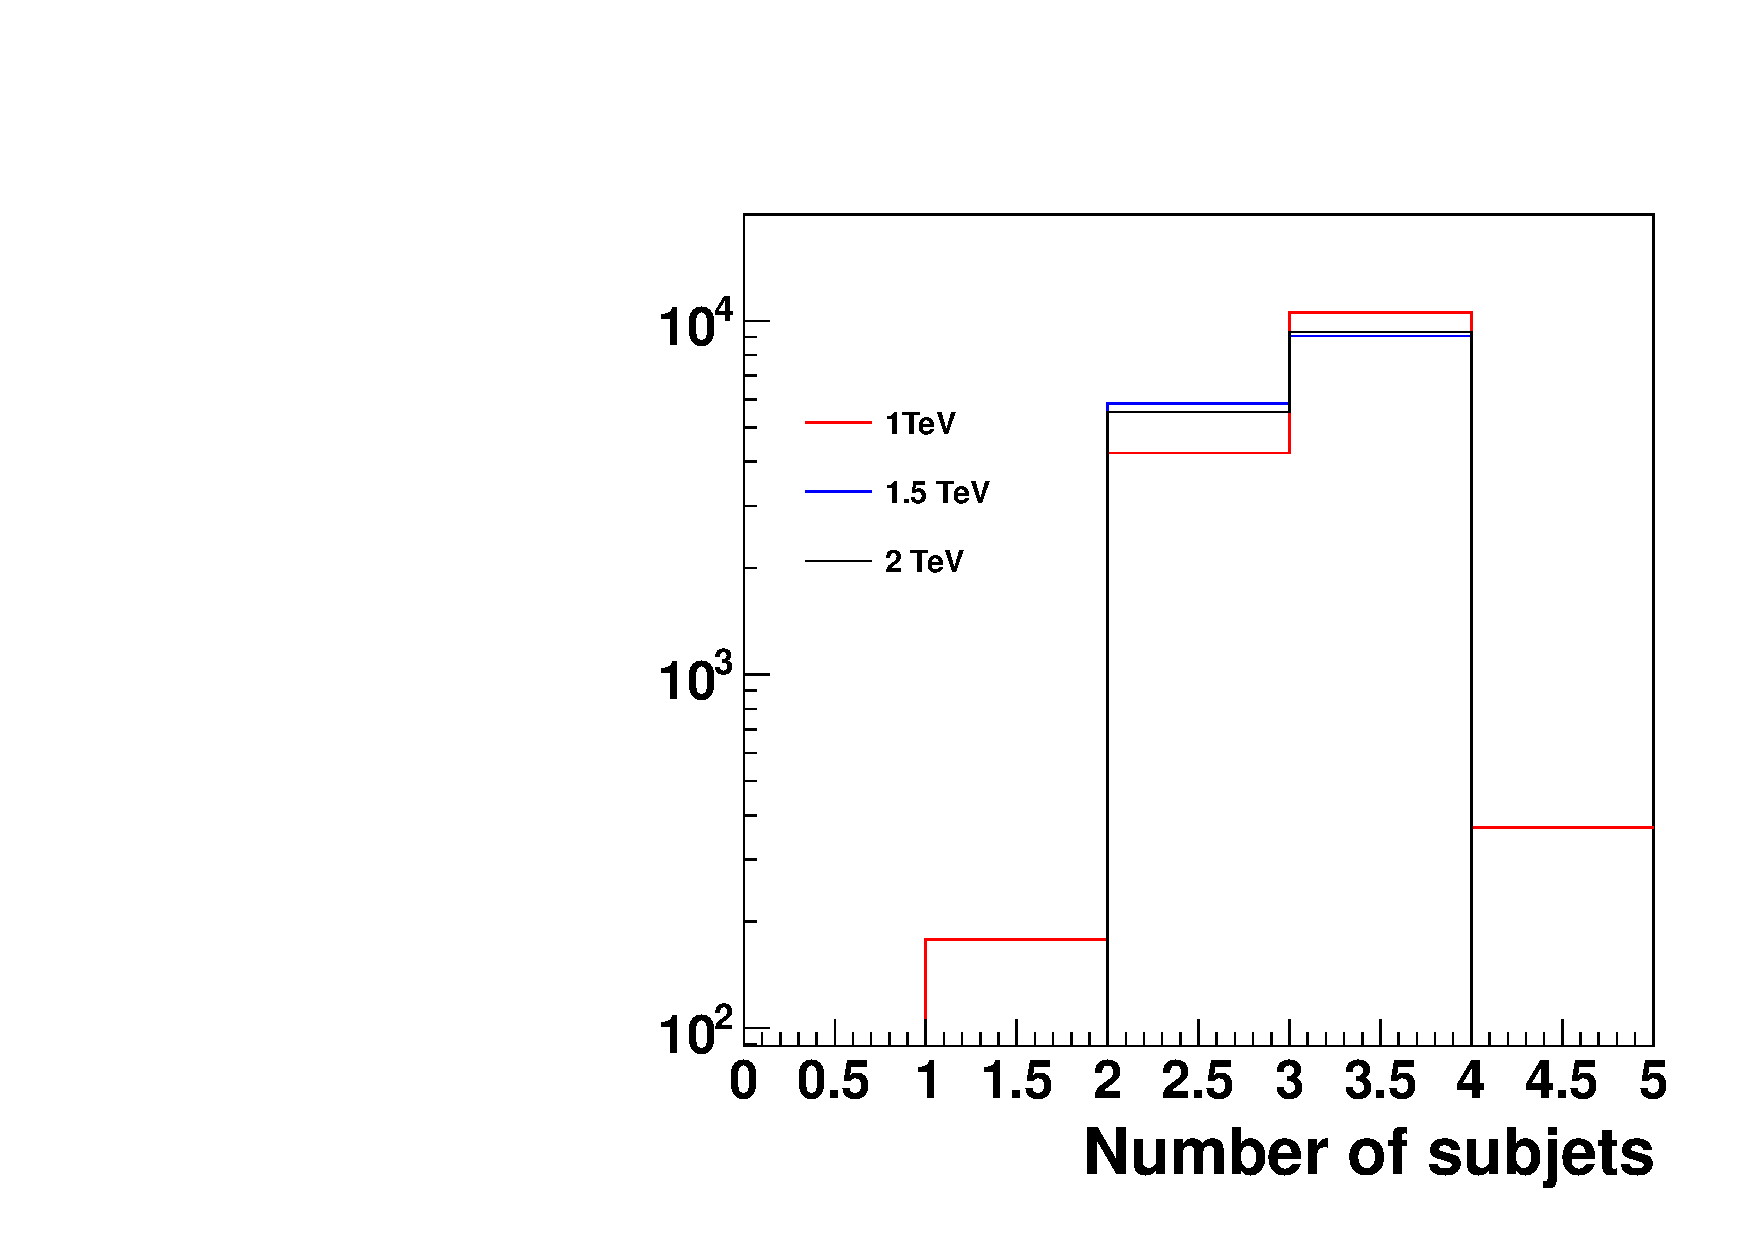
\includegraphics{HqqqqZqqfigs/N-subjettiness/Nsubjets.pdf}} 
%     \resizebox{0.5\linewidth}{!}{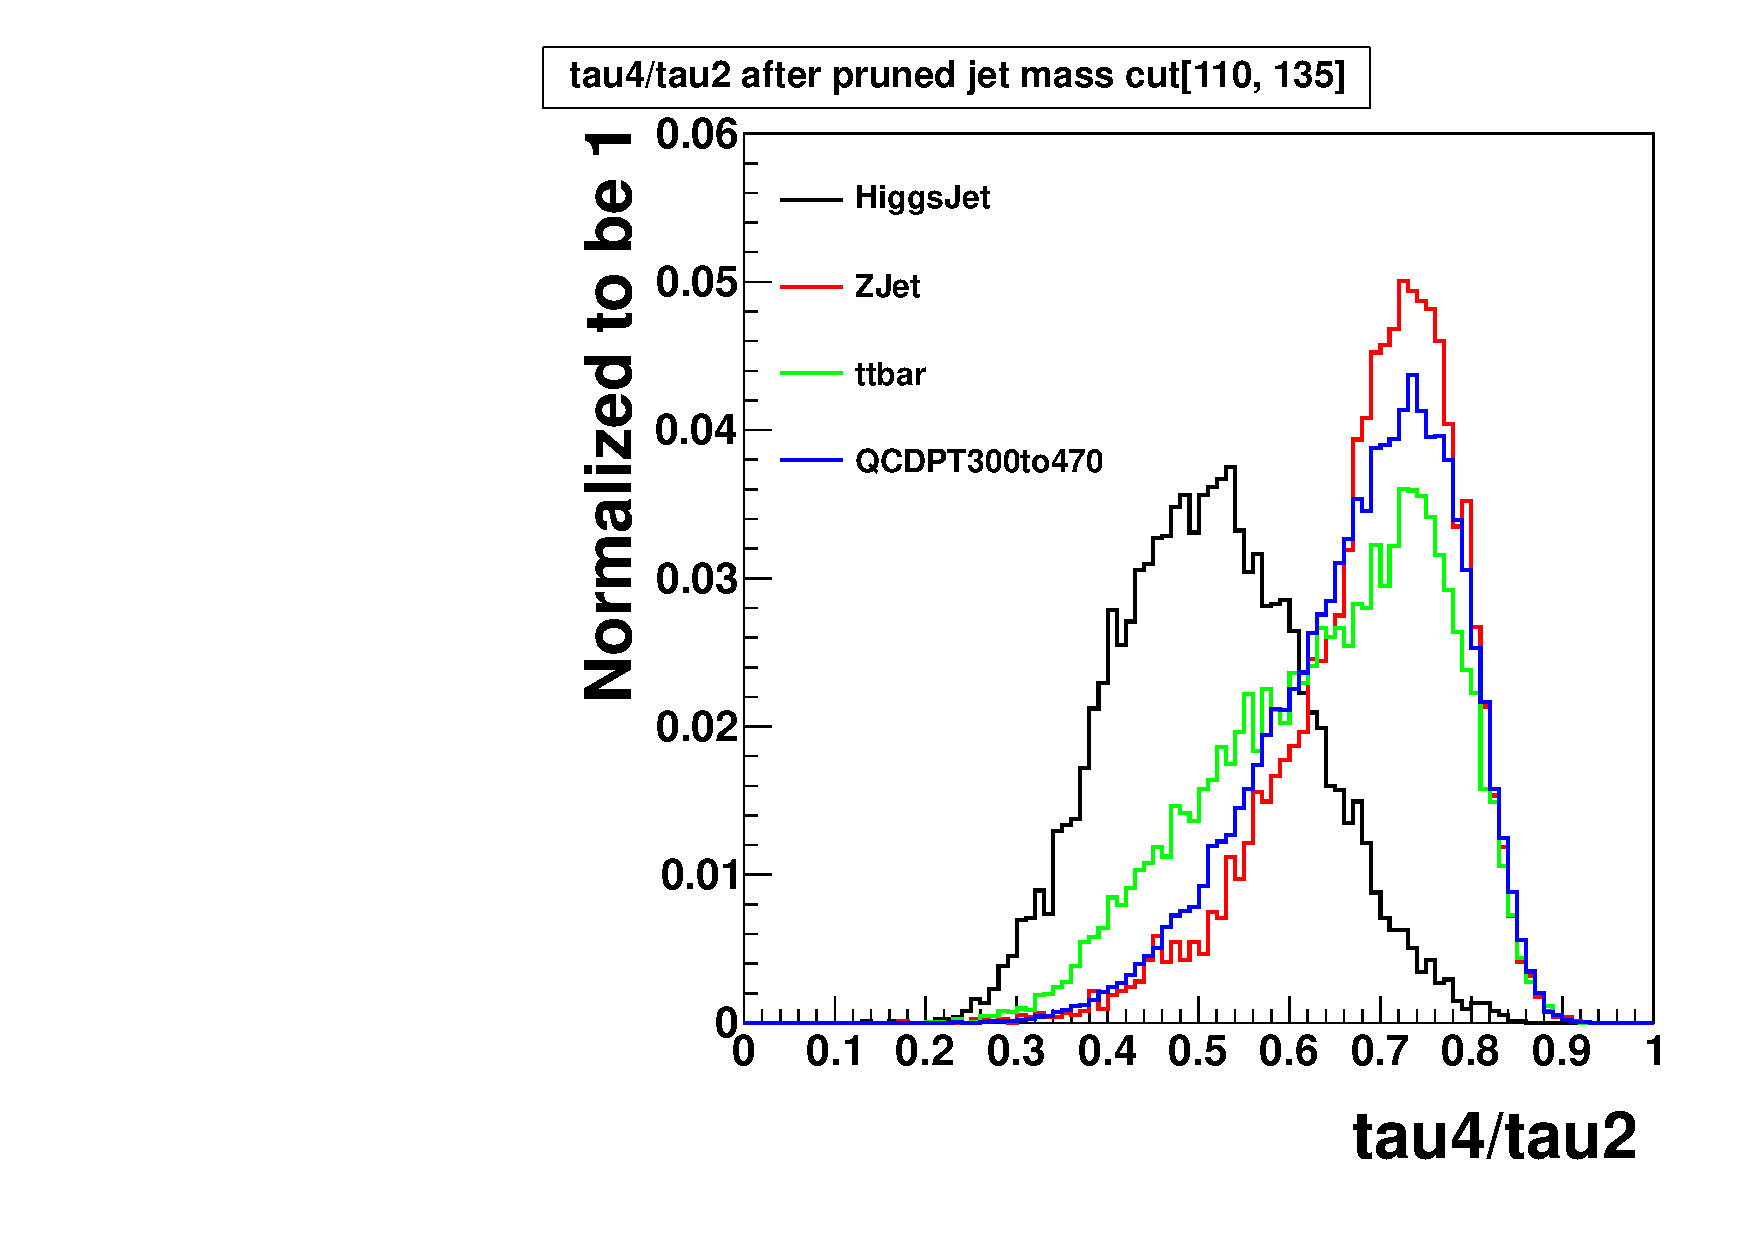
\includegraphics{HqqqqZqqfigs/N-subjettiness/Tau421TeVAfter.pdf}} \\
\end{tabular}
\caption{Number of subjets of the Higgs jets,  in \HwwVqq signal MC. 
Subjets are abtained from the CMSTopTag jet collection. }
\label{fig:Nsubjets}
\end{figure}


As an alternative, we explore the N-subjettiness, in particular the
variables involving $\tau_4$.  The ratio 
$\tau_{42} \equiv\tau_4/\tau_2$ has the best separation 
between the ${\rm H\to 4q}$
signal and not only QCD background, but also Z and top jets.
Figs~\ref{fig:tau421TeV} and~\ref{fig:tau422TeV} show the
discriminating power of $\tau_{42}$ against \ttbar and QCD, for 1~TeV
and 2~TeV resonance masses respectively.

\begin{figure}[htbp]
  \centering
  \begin{tabular}{cc}
    \resizebox{0.5\linewidth}{!}{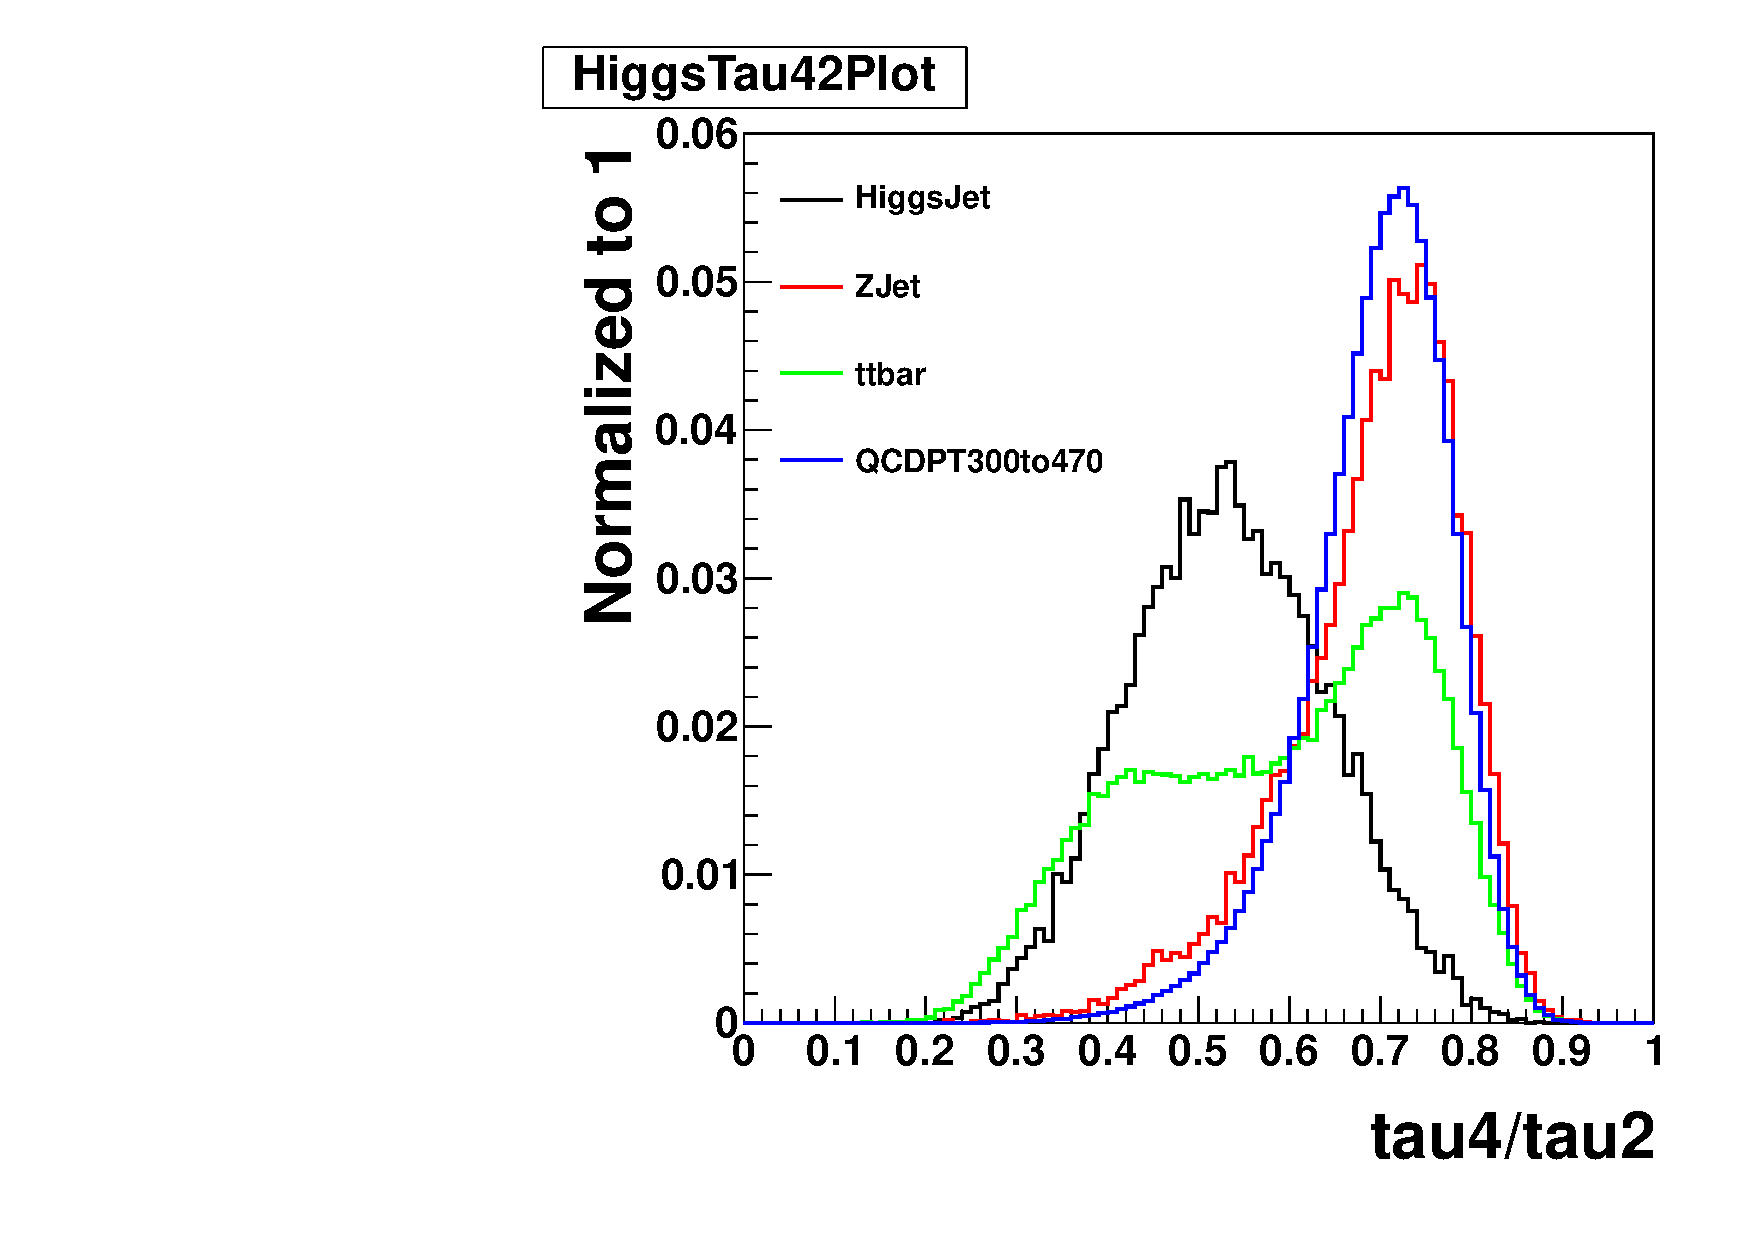
\includegraphics{HqqqqZqqfigs/N-subjettiness/Tau421TeVPre.pdf}} &
    \resizebox{0.5\linewidth}{!}{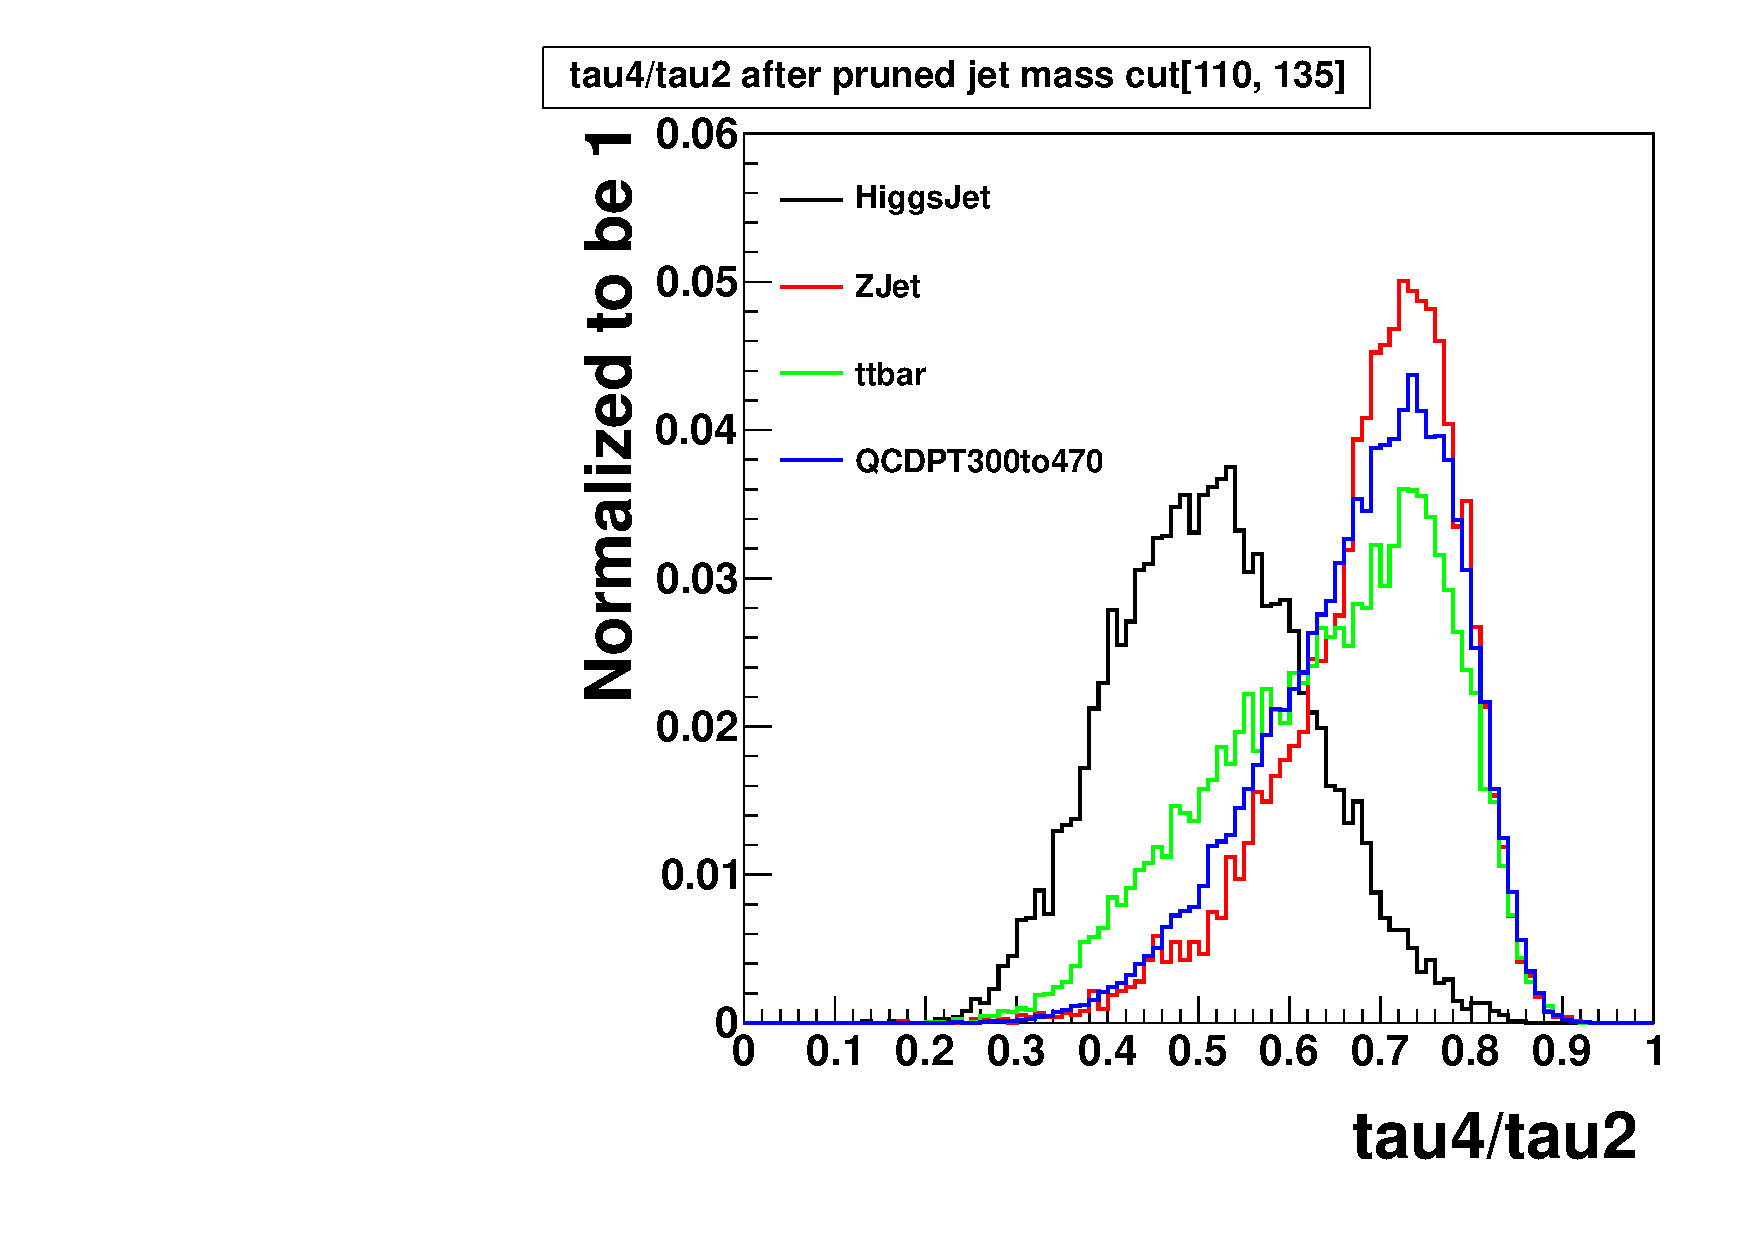
\includegraphics{HqqqqZqqfigs/N-subjettiness/Tau421TeVAfter.pdf}} \\
  \end{tabular}
  \caption{ 
    Distribution for $\tau_{4}/\tau_{2}$ in data and in
    simulations of signal (1.0 TeV) and background events.  All simulated
    distributions are scaled to match the number of events in data,
   % except that matched top is scaled to its fraction of unmatched
   %$ ${\rm t\bar{t}}$ times the number of data events.  
    W/Z, matched
    top and Higgs jets are required to match their generator level
    particles, respectively. }
  \label{fig:tau421TeV}
\end{figure}

\begin{figure}[htbp]
  \centering
  \begin{tabular}{cc}
    \resizebox{0.5\linewidth}{!}{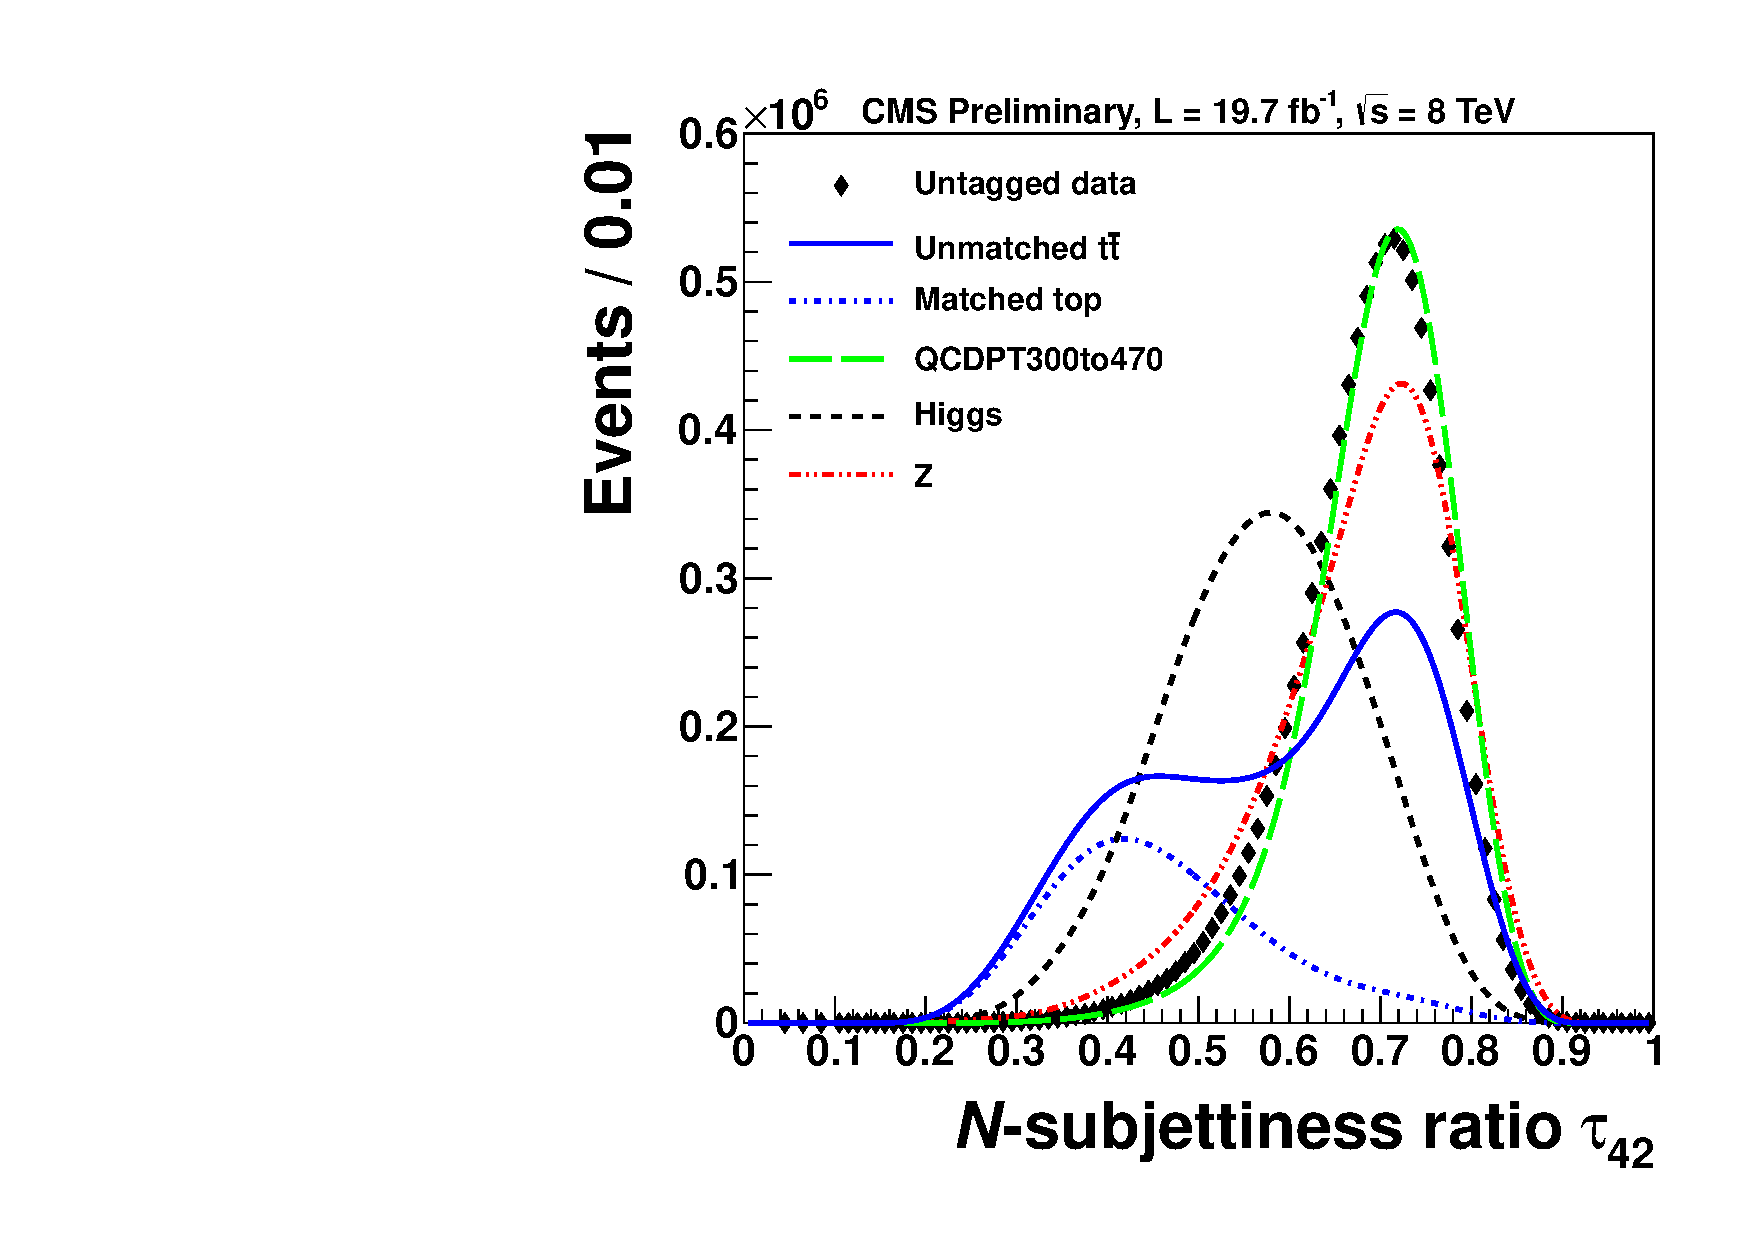
\includegraphics{HqqqqZqqfigs/N-subjettiness/tau42PlotAllPre.pdf}} &
    \resizebox{0.5\linewidth}{!}{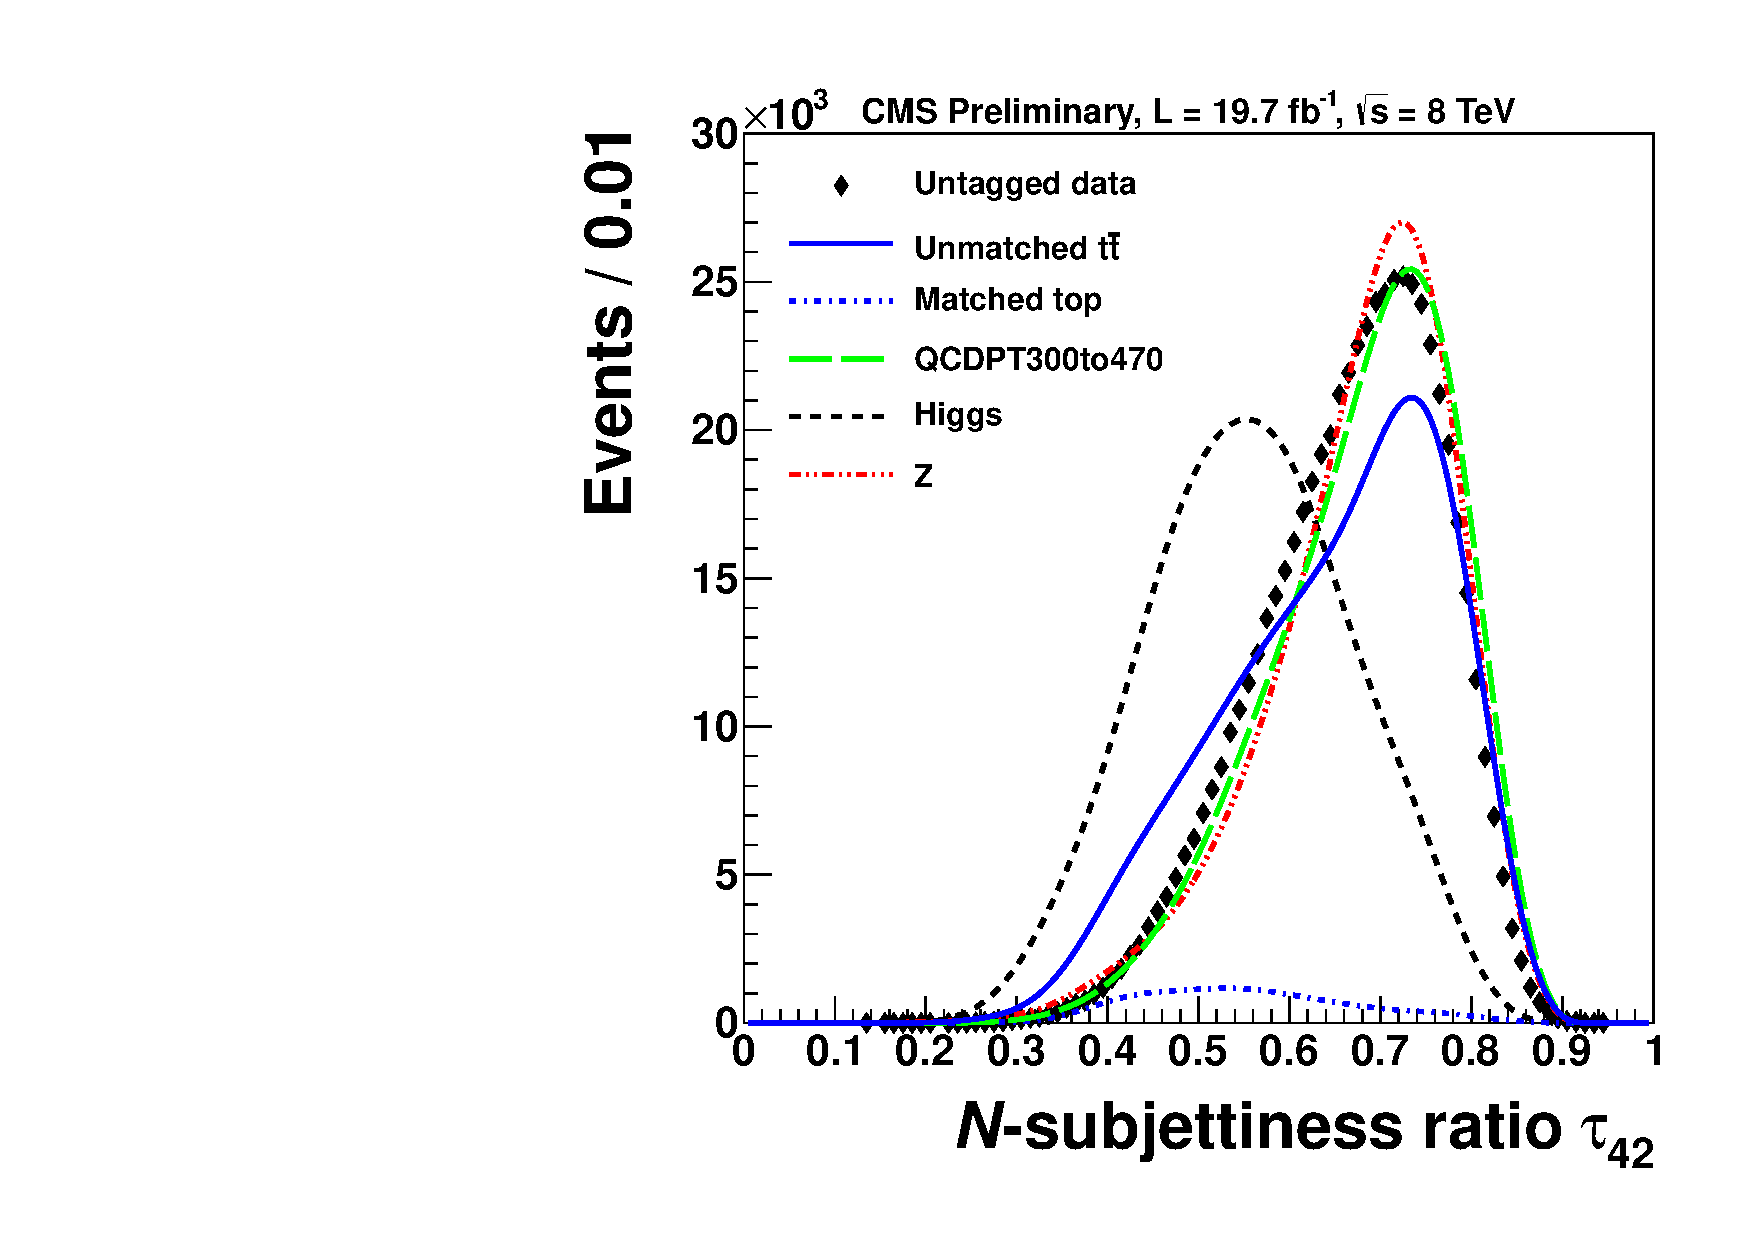
\includegraphics{HqqqqZqqfigs/N-subjettiness/tau42PlotAllAfter.pdf}} \\
  \end{tabular}
  \caption{ Distribution for $\tau_{4}/\tau_{2}$ in data and in
    simulations of signal (2.0 TeV) and background events.  All simulated
    distributions are scaled to match the number of events in data,
    except that matched top is scaled to its fraction of unmatched
    ${\rm t\bar{t}}$ times the number of data events.  W/Z, matched
    top and Higgs jets are required to match their generator level
    particles, respectively.  }
  \label{fig:tau422TeV}
\end{figure}

We also explore other combinations of $\tau_{NM} \equiv \tau_N/\tau_M $,
which are listed in Appendix.~\ref{appendix:tauNM}.
The ROC (receiver operating characteristic) 
curve of for several $\tau_{NM}$ cuts (but the same pruned jet mass cut)
is shown in Fig.~\ref{fig:roc}.  The signal efficiency is evaluated
using Higgs jets in 2 \TeV signal MC, and the false positive rate
({\it i.e.}, mistag rate) is derived from QCDPT300to470 MC sample.
From the figure, it is clear that $\tau_{42}$ outperforms any other
single $\tau_{NM}$ variable.
%
%
\begin{figure}[htbp]
  \centering
  \begin{tabular}{cc}
    \resizebox{0.7\linewidth}{!}{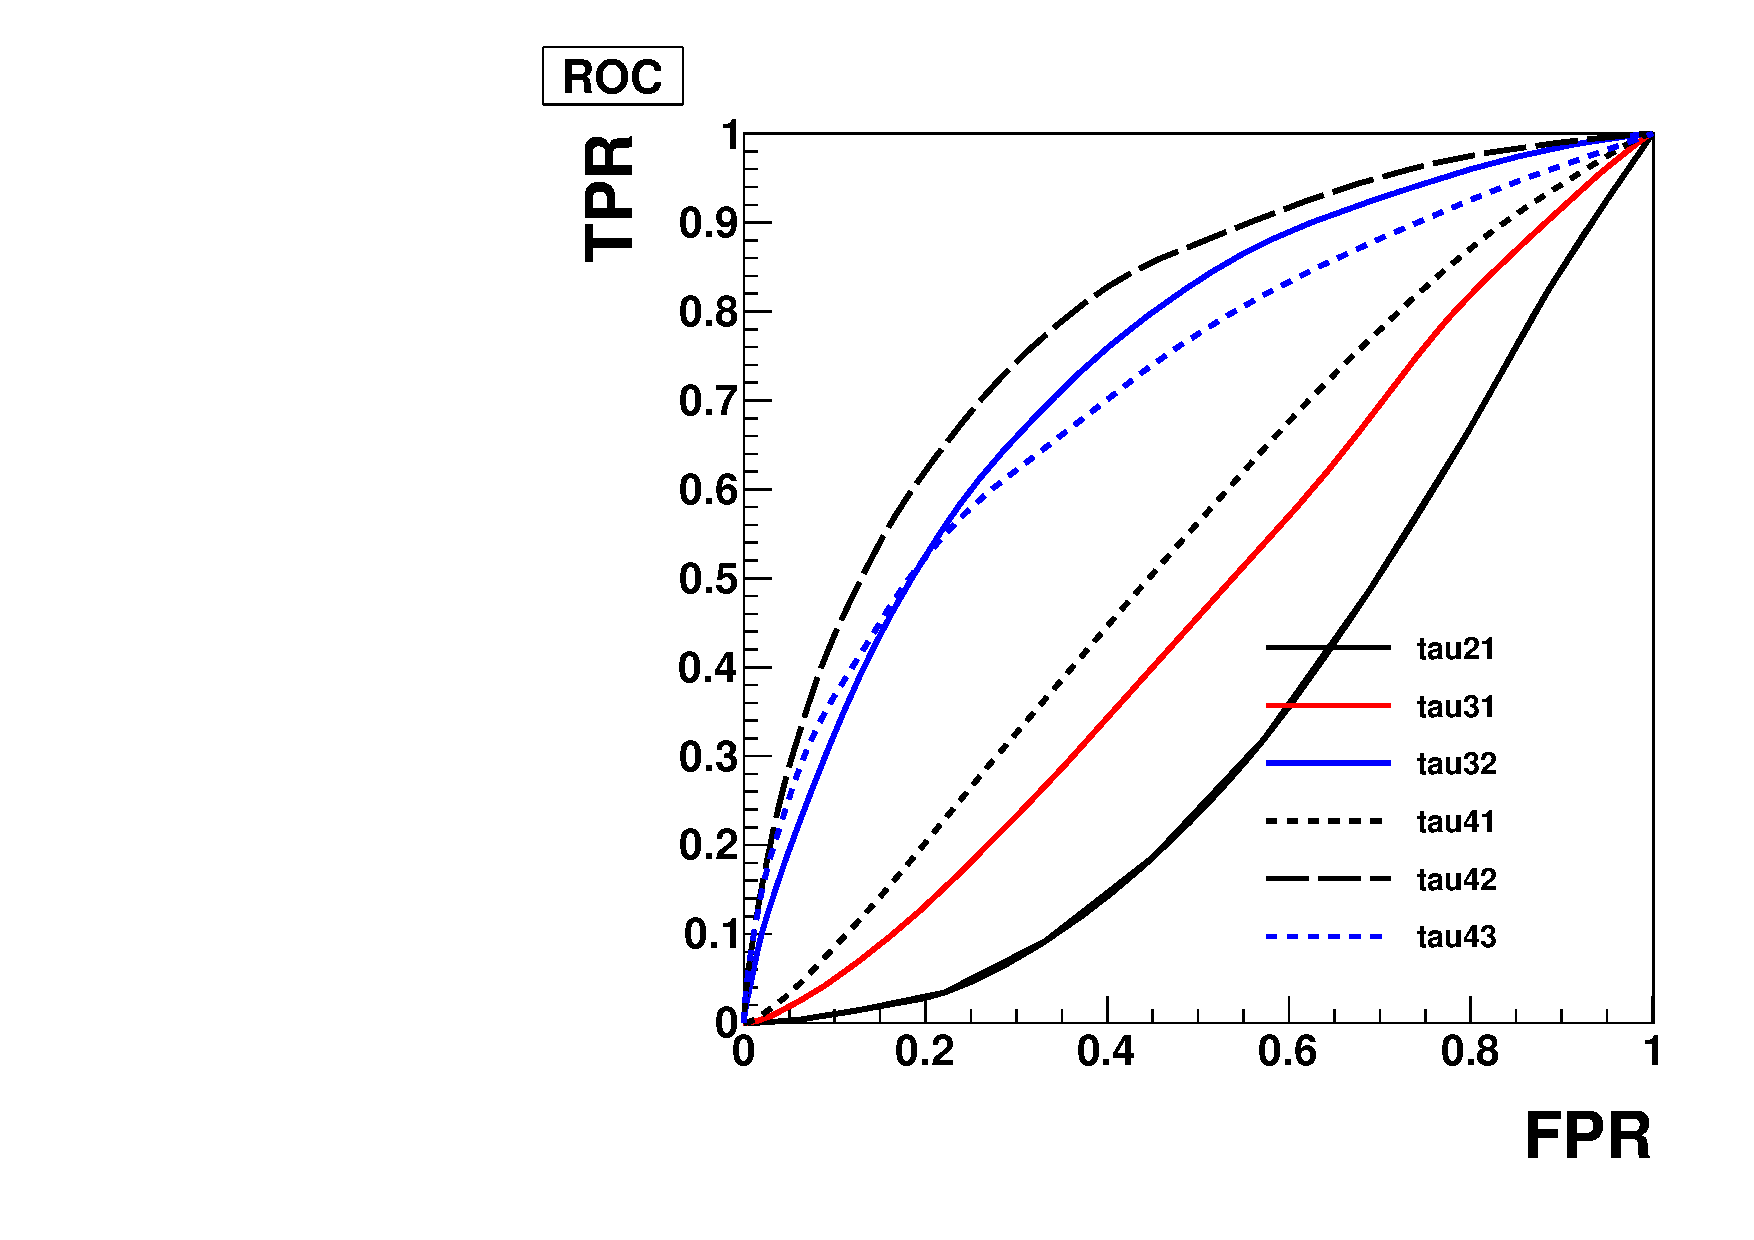
\includegraphics{ROC.pdf}} 
    %     \resizebox{0.5\linewidth}{!}{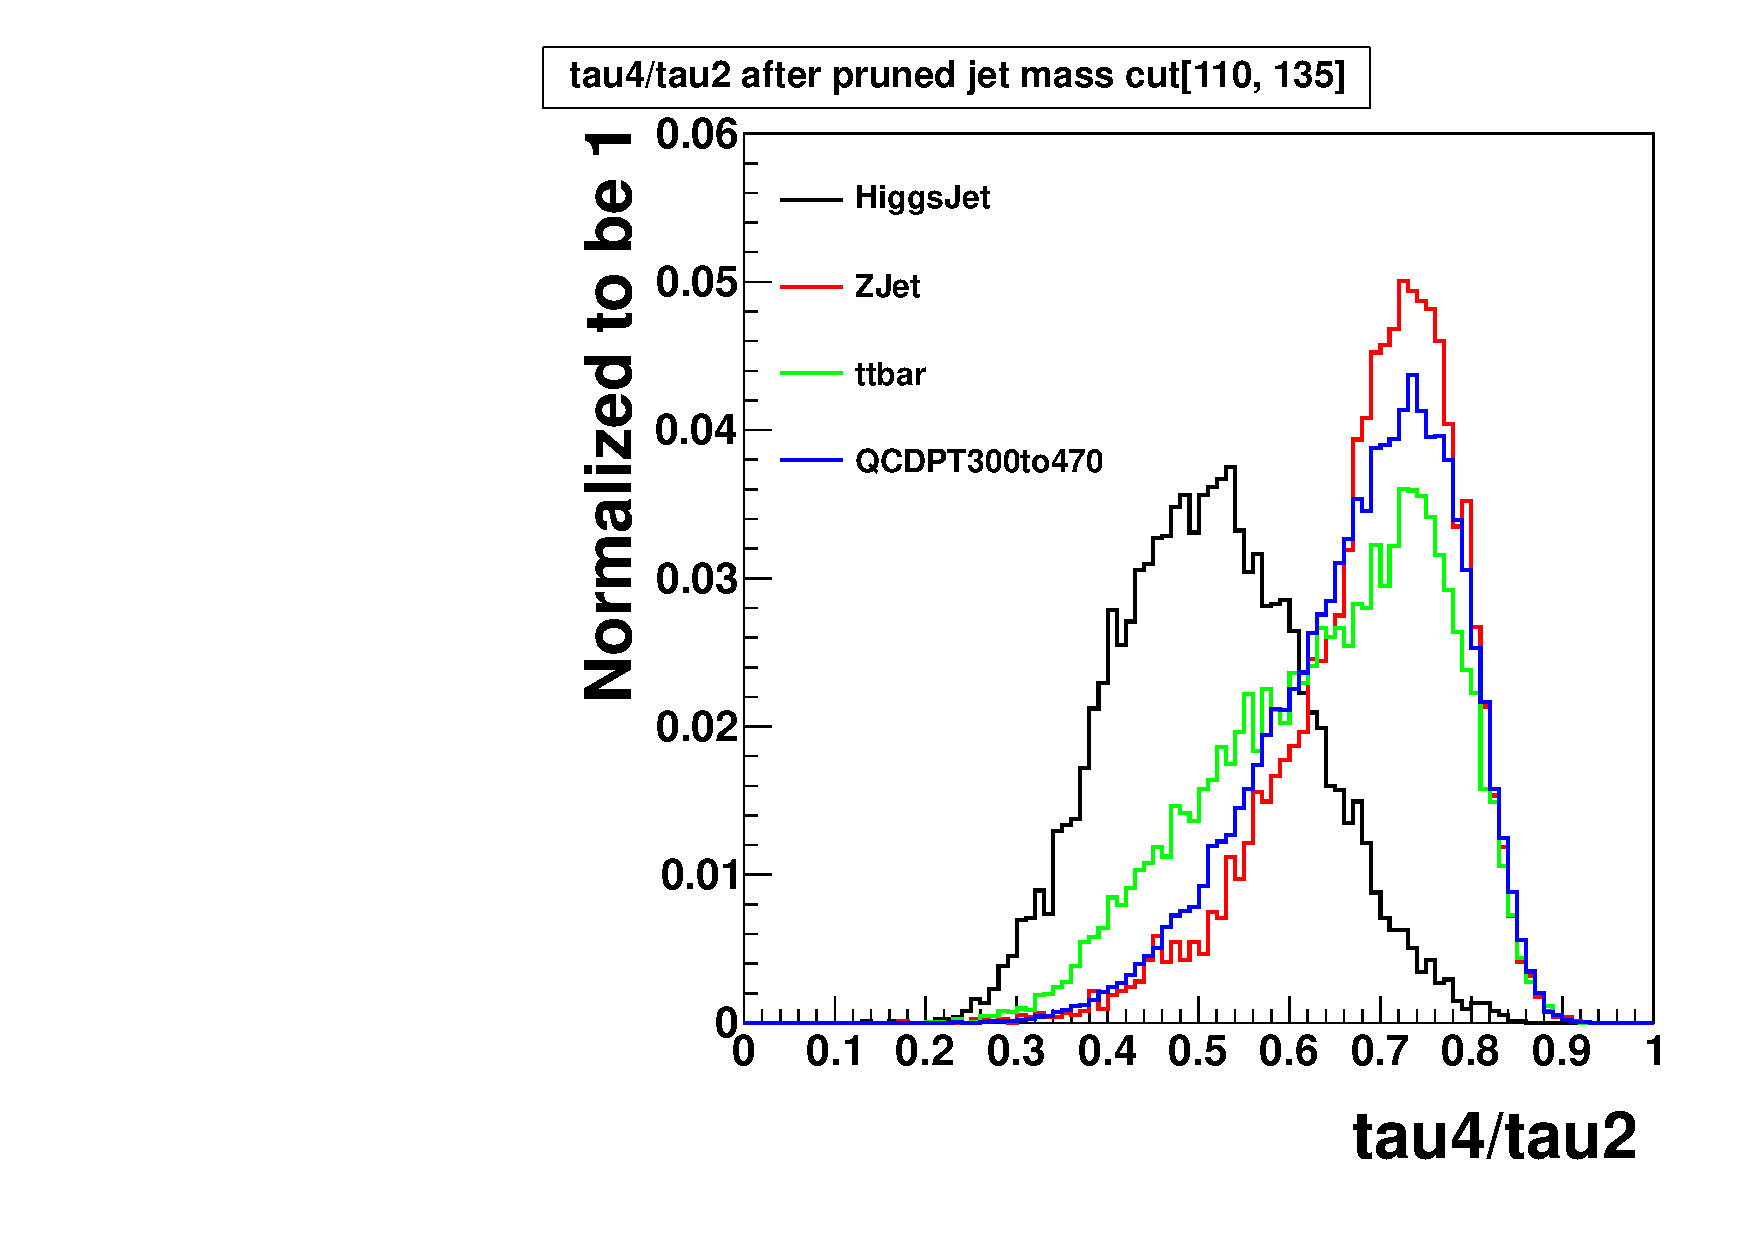
\includegraphics{HqqqqZqqfigs/N-subjettiness/Tau421TeVAfter.pdf}} \\
  \end{tabular}
  \caption{ ROC curves for different $\tau_{NM}$ after the cut on the
    pruned jet mass.  The false positive rate (FPR) is obtained from
    QCDPT300to470 and the true positive rate (TPR) from Higgs jets
    in 2 \TeV signal MC sample.  Using $\tau_{42}$ to select Higgs
    jets outperforms all other $\tau_{NM}$ variables. }
  \label{fig:roc}
\end{figure}



After optimizing the cut on $\tau_{42}$ (documented in
Sec.~\ref{sec:tau42Opti} below), the full selection of the ${\rm H \to
  WW^* \to 4q}$ tagger is:
\begin{itemize}

\item {\bf Pruned jet mass}  $\mbox{\boldmath$m_{\text{jet}}$}$
  - We require the total pruned jet mass to satisfy $110 \GeVcc < m_\text{jet} <  135 \GeVcc $.

\item {\bf N-subjettiness}
  - We split the events into two categories, ``high purity'' Higgs jets by
    requiring $\tau_{42} \leq 0.55$, while $ 0.55 < \tau_{42} < 0.65$ defines
    the ``low purity'' Higgs jets.  

\end{itemize}
 



\clearpage

%\subsection{$\tau_4/\tau_2$ optimization study}
\subsubsection{Optimization of the $\tau_4/\tau_2$ threshold}
\label{sec:tau42Opti}


Having selected $\tau_{42}$ as the discriminating variable, we next
optimize its upper value.  In this study, the jet mass is confined
within $[110, 135]~\GeV$.  We use the limit setting method (described
in Sec.~\ref{sec:statistics}) and evaluate the expected limits of
several signal resonance masses at different $\tau_{42}$ working
points.  These expected limits are presented
in Table.~\ref{table:tau42Opti}.
Given our focus on the resonance masses above 1500~\GeV, we
choose to cut on $\tau_{42} < 0.55$. In the following analysis, 
to compensate the signal efficiency loss at higher resonance mass, we 
introduce an additional categories for $\Hww$ tagger as $0.55 < \tau_{42} < 0.65$.
This is chosen from back-of-envelope calculation based on 
Figs~\ref{fig:tau421TeV} and~\ref{fig:tau422TeV}, since this category provides 
very limited sensitivity.  
%Figure~\ref{}i 

\begin{table}[htbp]
\begin{center}
\topcaption{Upper limits (in units of 0.01~pb) 
for high purity HW and HZ signals at different resonance masses and also
different $\tau_{42}$ working points. }
\label{table:tau42Opti}
\begin{tabular}{|r|r|r|r|r|}
\hline
\multicolumn{1}{|l|}{HW / $\tau_{42}$} & 0.45 & 0.5 & 0.55 & 0.6 \\ 
1000 & 4.14 & 4.09 & 4.46 & 4.91 \\ 
1500 & 0.97 & 0.88 & 0.86 & 0.91 \\ 
2000 & 0.89 & 0.64 & 0.51 & 0.47 \\ 
2500 & 1.36 & 0.82 & 0.53 & 0.40 \\ \hline 
\multicolumn{1}{|l|}{HZ / $\tau_{42}$} & \multicolumn{1}{l|}{} & \multicolumn{1}{l|}{} & \multicolumn{1}{l|}{} & \multicolumn{1}{l|}{} \\ 
1000 & 4.31 & 4.36 & 4.63 & 5.05 \\ 
1500 & 0.98 & 0.89 & 0.86 & 0.90 \\ 
2000 & 0.70 & 0.55 & 0.42 & 0.39 \\ 
2500 & 0.96 & 0.61 & 0.41 & 0.32 \\ \hline
\end{tabular}
\end{center}
\end{table}



%\subsection{Summary of Higgs and W/Z tagging categories}
%\label{sec:total}

%In summary, the W or Z jets from the signal are selected by the
%V-tagger, and the Higgs candiadates are selected by an OR of the two
%Higgs taggers, $\Hbb$ and $\Hww$.  Both V-tagger and $\Hww$ taggers 
%have high-purity and
%low-purity categories.  The latter are added to increase the
%sensitivity of the analysis at high resonance masses, where the QCD
%background is low, and a higher signal efficiency is at the premium.
%All the `two-dimensional' categories are shown in
%Table~\ref{table:categories}.  For the \HwwVqq\ channel, we drop the
%low-purity Higgs and low-purity V-tagging category, because it 
%adds only a negligible sensitivity.

%\begin{table}[htb]
%\begin{center}
%  \topcaption{
%    The five event categories used in this analysis.
%    \label{table:categories}}
%\begin{tabular}{ ccc}
%\hline
%$\Hbb$, $\Vqq$ & $\Hww$, $\Vqq$  \\
%\hline
%high-purity V-tag &  high-purity H-tag, high-purity V-tag \\
%low-purity  V-tag &  high-purity H-tag, low purity V-tag\\
%                  &  high-purity V-tag, low purity H-tag\\
%\hline
%\end{tabular}
%\end{center}
%\end{table}




\iffalse

\begin{table}[htbp]
\begin{tabular}{|r|r|r|r|r|r|r|}
\hline
\multicolumn{1}{|l|}{$\tau_{42}$} & \multicolumn{1}{l|}{1000GeV} & \multicolumn{1}{l|}{1500GeV} & \multicolumn{1}{l|}{1800GV} & \multicolumn{1}{l|}{2000GeV} & \multicolumn{1}{l|}{2500GeV} & \multicolumn{1}{l|}{3000GeV} \\ \hline
0.60 & 49.90 & 44.10 & 38.05 & 33.58 & 21.45 & 11.08 \\ \hline
0.55 & 54.20 & 45.33 & 38.52 & 33.91 & 20.88 & 10.69 \\ \hline
0.50 & 55.81 & 45.51 & 37.97 & 32.22 & 19.98 & 9.70 \\ \hline
0.45 & 55.91 & 43.12 & 35.28 & 29.06 & 17.80 & 8.43 \\ \hline
0.40 & 49.17 & 35.99 & 31.21 & 24.55 & 14.13 & 6.73 \\ \hline
0.35 & 37.64 & 28.42 & 22.15 & 18.95 & \multicolumn{1}{l|}{} & \multicolumn{1}{l|}{} \\ \hline
\end{tabular}
\caption{Optimization for $\tau_{42}$ tagger, with a fixed pruned jet 
  mass in $[110~GeV/c^2, 135~GeV/c^2]$.  The table shows the ratio of 
  the number of signal events(without normalization) divided by the number of signal+background
  events(data).}
\label{table:tau42Opti}
\end{table}

\fi



\clearpage


%\input{H-taggingAlgo2.tex}
%% &&& Petar: no need for this now:  
%% \newpage
\section{Data and MC comparisons}
\label{sec:data-mc-comp}

In this section, we compare some kinematic features of the jets between QCD MC and data, which are
 shown in Fig~\ref{fig:mjjSingle}, \ref{fig:mjjDouble},\ref{fig:dySingle}, \ref{fig:dyDouble}, \ref{fig:dphiSingle}, 
\ref{fig:dphiDouble},\ref{fig:metSumPtSingle},
\ref{fig:Pt0Single}, \ref{fig:Pt0Double}, \ref{fig:Pt1Single}, \ref{fig:Pt1Double},
\ref{fig:Eta0Single}, \ref{fig:Eta0Double}, \ref{fig:Eta1Single}, \ref{fig:Eta1Double},
%\ref{fig:CA8Single},\ref{fig:CA8Double}
and \ref{fig:massNsub}.
Predictions from Pythia6 with Tune $Z2*$ and Herwig++ with Tune 23 are shown.
The comparison is shown in the exclusive dijet category, low and high purity,  single and double tagged events..
The distributions are shown after the event selection (in particular $|y| < 2.5$, $|\Delta\eta|<1.3$, $m_{jj} > 890  \GeVcc$) is applied.
The number of data events in each mass bin are shown in Table~\ref{table:eventnumbers}.
The MC is normalized to the number of data events in each category and the shapes are compared.


\begin{table}[htb]
%\begin{center}
\begin{tabular}{|p{3.0cm}|p{3.0cm}|p{3.0cm}|p{3.0cm}|p{3.0cm}|}
%\begin{tabular}{|c|c|c|c|c|}
\hline
lower mass bin border & low purity 1-tag events & high purity 1-tag events& low purity 2-tag events& high purity 2-tag events\\
\hline
890 & 165671 & 105892 & 7586 & 2544 \\ 
944 & 115622 & 72007 & 4950 & 1673 \\ 
1000 & 80537 & 48930 & 3311 & 1005 \\ 
1058 & 56423 & 33398 & 2159 & 658 \\ 
1118 & 39817 & 23086 & 1407 & 427 \\ 
1181 & 27651 & 15817 & 962 & 302 \\ 
1246 & 19531 & 10741 & 647 & 175 \\ 
1313 & 13617 & 7477 & 434 & 135 \\ 
1383 & 9880 & 5128 & 272 & 75 \\ 
1455 & 6992 & 3578 & 195 & 49 \\ 
1530 & 4939 & 2525 & 138 & 25 \\ 
1607 & 3443 & 1658 & 86 & 24 \\ 
1687 & 2454 & 1160 & 52 & 10 \\ 
1770 & 1744 & 815 & 42 & 9 \\ 
1856 & 1193 & 547 & 35 & 6 \\ 
1945 & 881 & 389 & 21 & 4 \\ 
2037 & 643 & 230 & 12 & 3 \\ 
2132 & 402 & 167 & 8 & 3 \\ 
2231 & 287 & 99 & 5 & 1 \\ 
2332 & 193 & 86 & 3 &  \\ 
2438 & 138 & 57 & 1 &  \\ 
2546 & 87 & 28 & 0 &  \\ 
2659 & 60 & 13 & 2 &  \\ 
2775 & 48 & 11 &  &  \\ 
2895 & 38 & 5 &  &  \\ 
3019 & 14 & 4 &  &  \\ 
3147 & 17 & 3 &  &  \\ 
3279 & 4 & 1 &  &  \\ 
3416 & 4 & 0 &  &  \\ 
3558 & 4 & 1 &  &  \\ 
3704 &  & 1 &  &  \\ 
3854 &  &  &  &  \\ 
4010 &  &  &  &  \\ 
\hline
\end{tabular}
\caption{Number of events in each mass bin exclusive, with 1 W/Z-tag and  2 W/Z-tags required in low
purity and high purity categories.}
\label{table:eventnumbers}
\end{table}



\newpage


\begin{figure}[htb]
\centering
\begin{tabular}{cc}
     \resizebox{0.5\linewidth}{!}{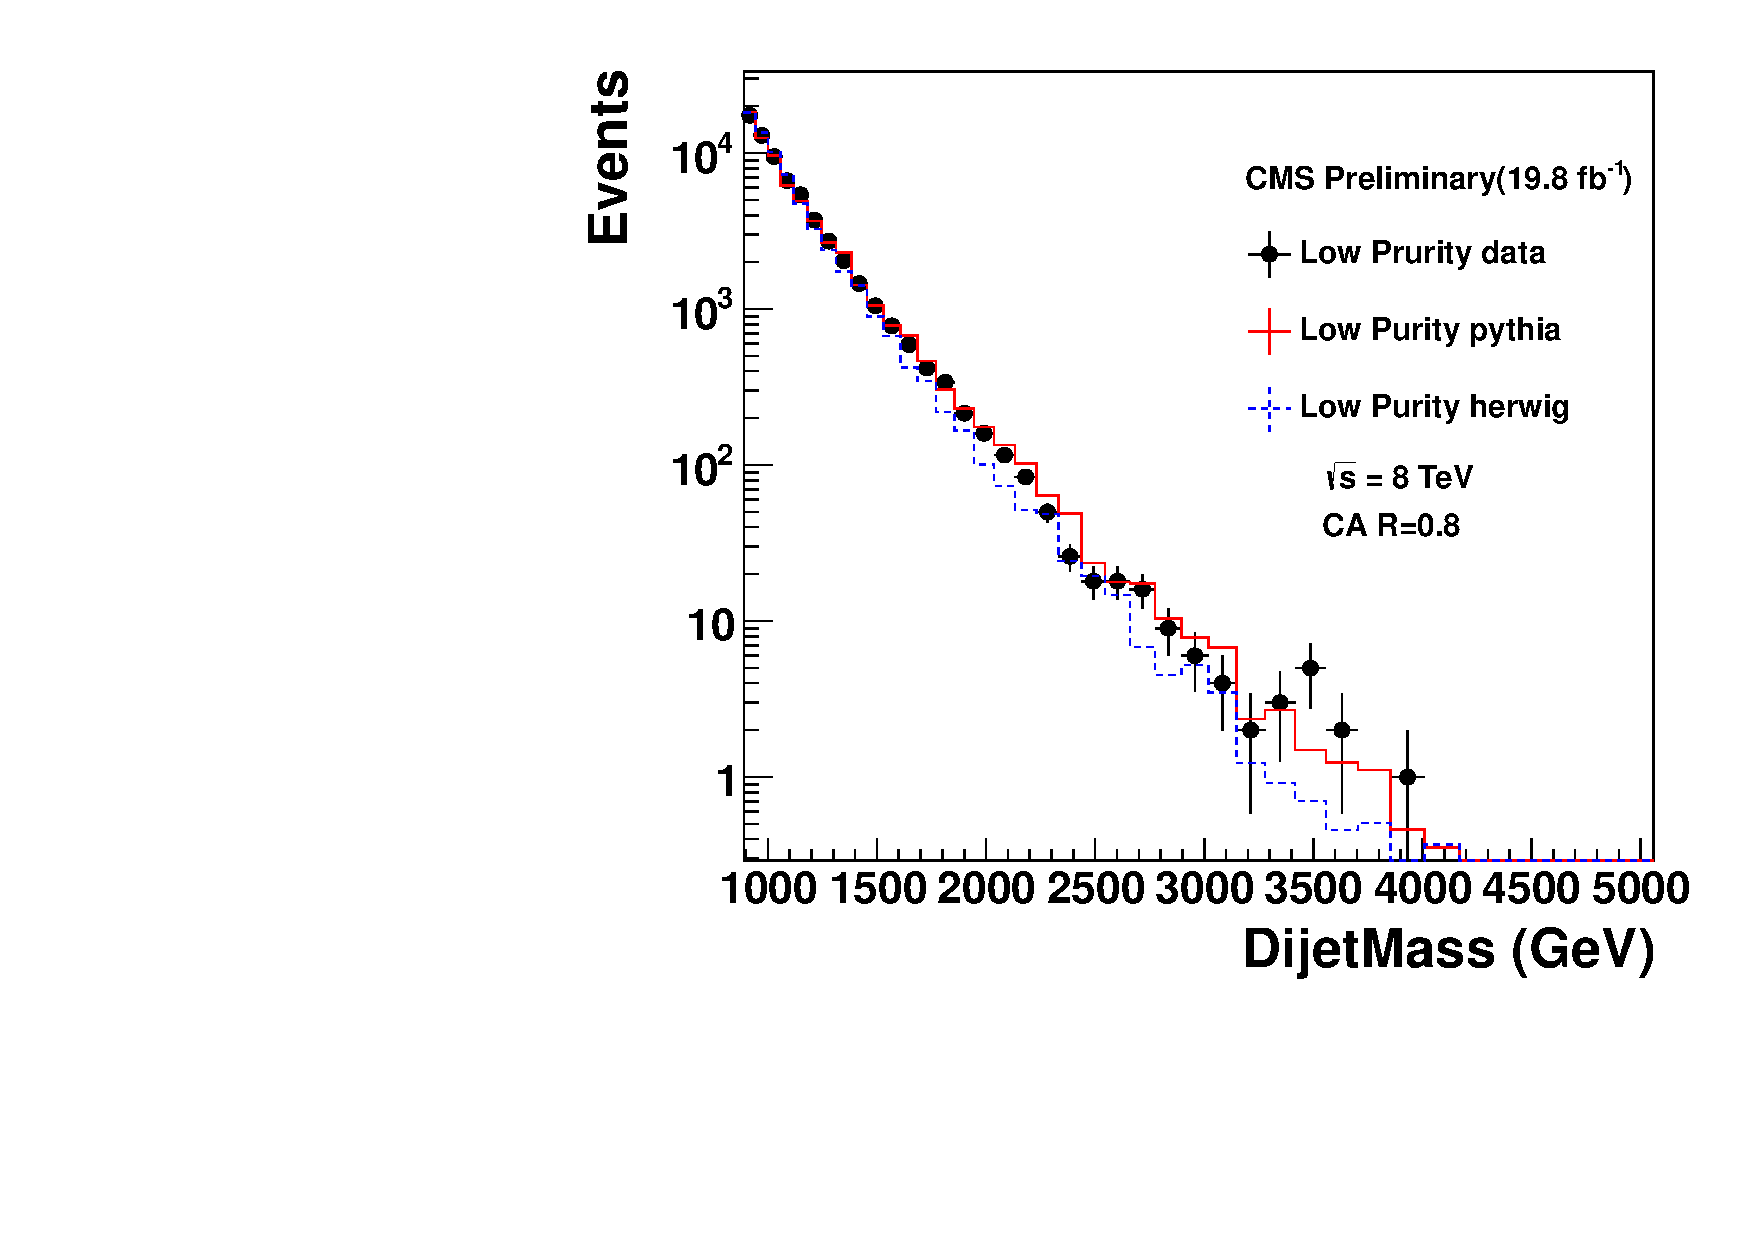
\includegraphics{figs/Data-MC-comparisons/DijetMass-qVLowP.pdf}} &
     \resizebox{0.5\linewidth}{!}{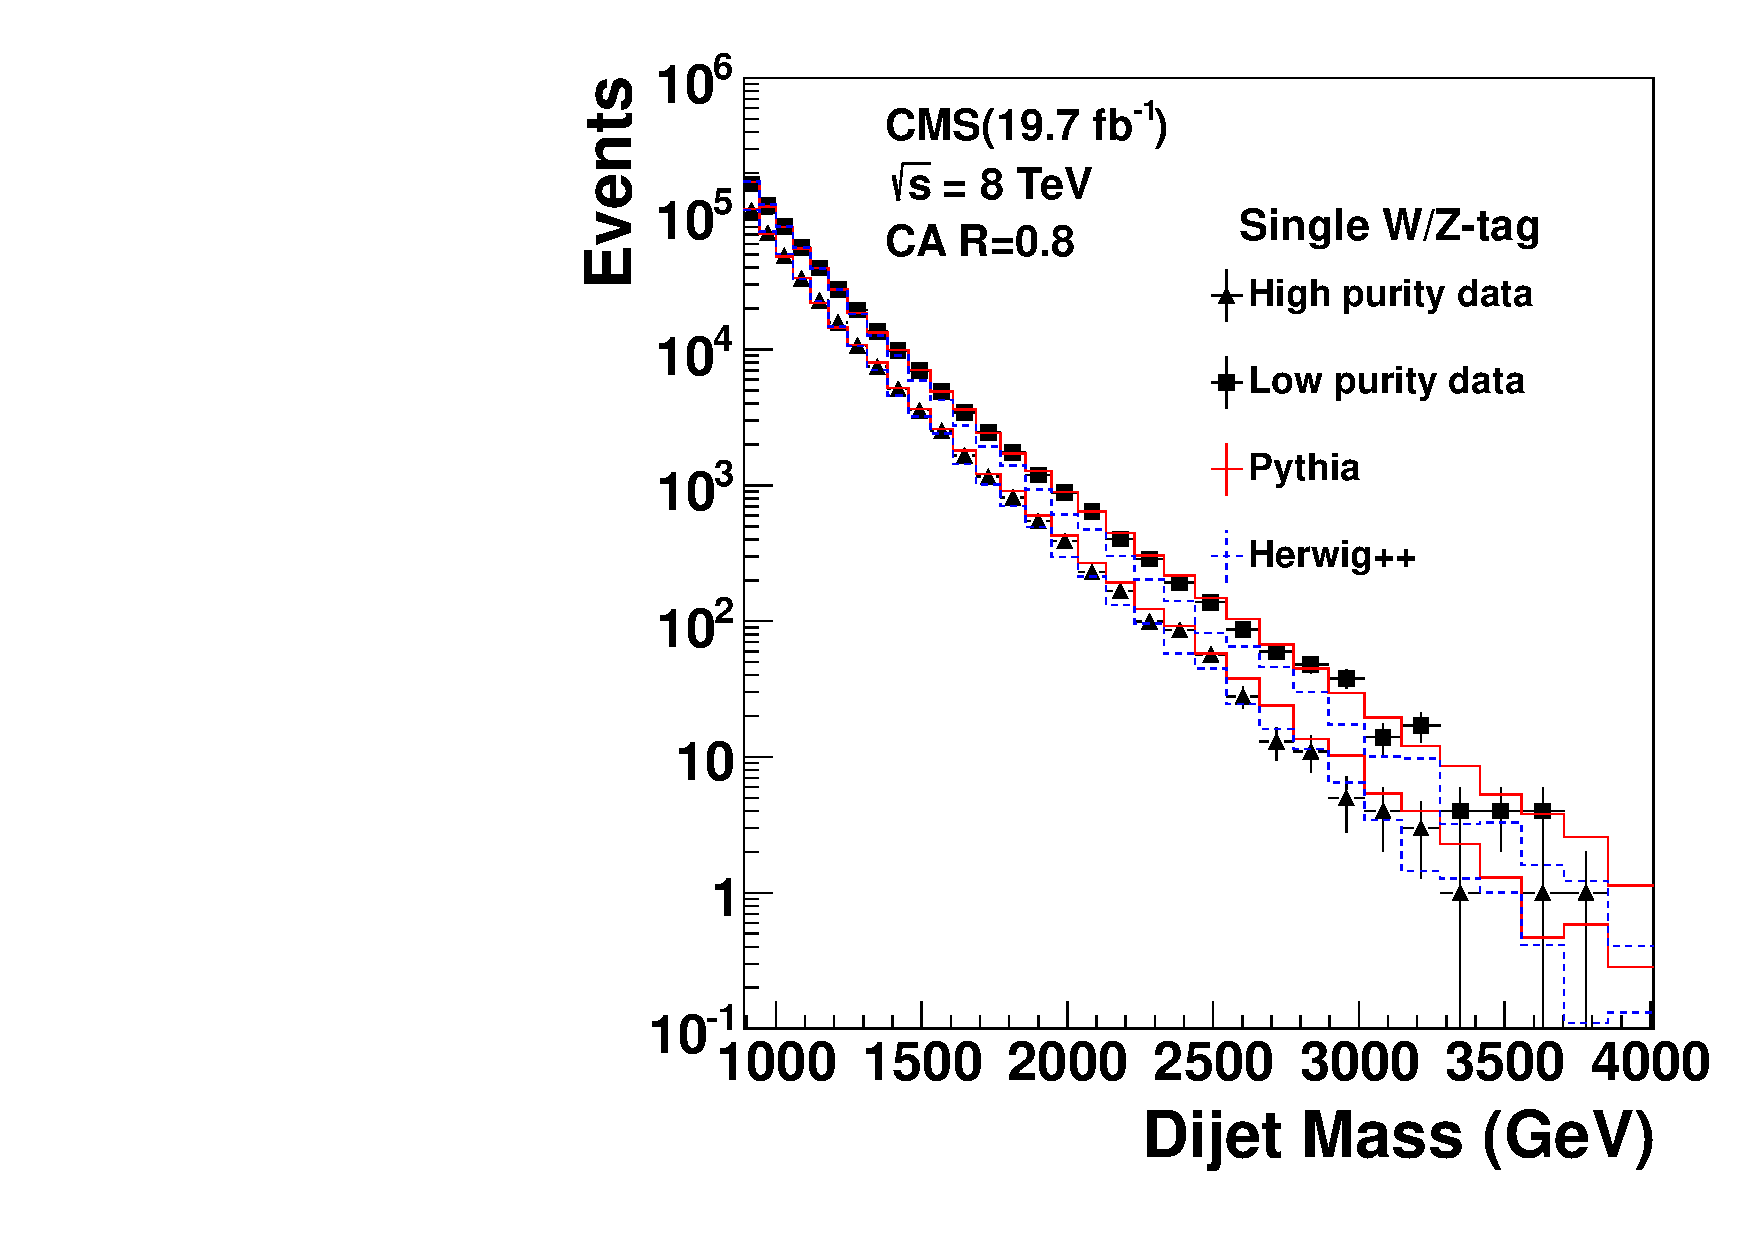
\includegraphics{figs/Data-MC-comparisons/DijetMass-qVMiumHigh.pdf}} \\
\end{tabular}
  \caption[Invariant Mass Single]{Comparisons between data and Monte Carlo
           for invariant mass of the two leading jets of low purity (left) and low-high purity (right) 1-tagged events.
           The MC is normalized to the number of data events in each category.
           }
  \label{fig:mjjSingle}
\end{figure}

\begin{figure}[htb]
\centering
\begin{tabular}{cc}
     \resizebox{0.5\linewidth}{!}{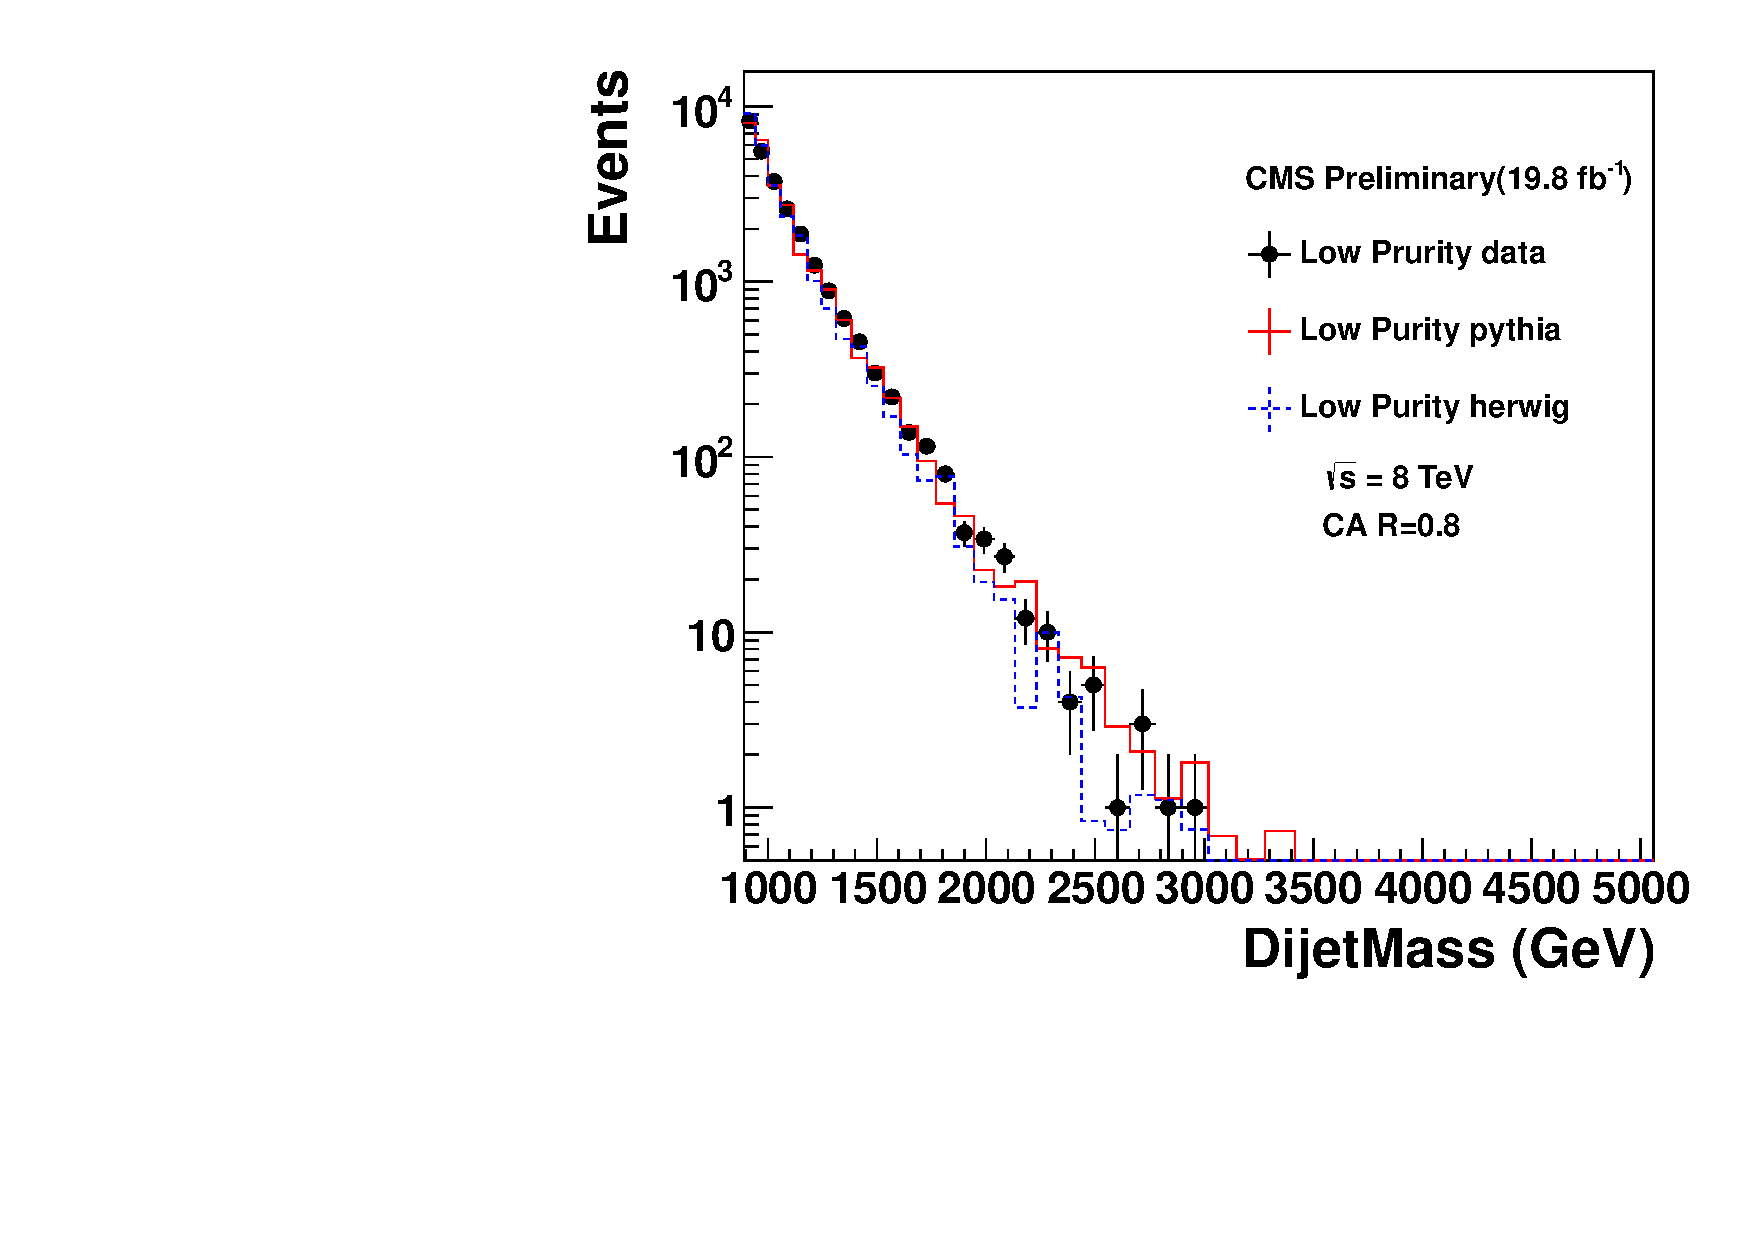
\includegraphics{figs/Data-MC-comparisons/DijetMass-VVLowP.pdf}} &
     \resizebox{0.5\linewidth}{!}{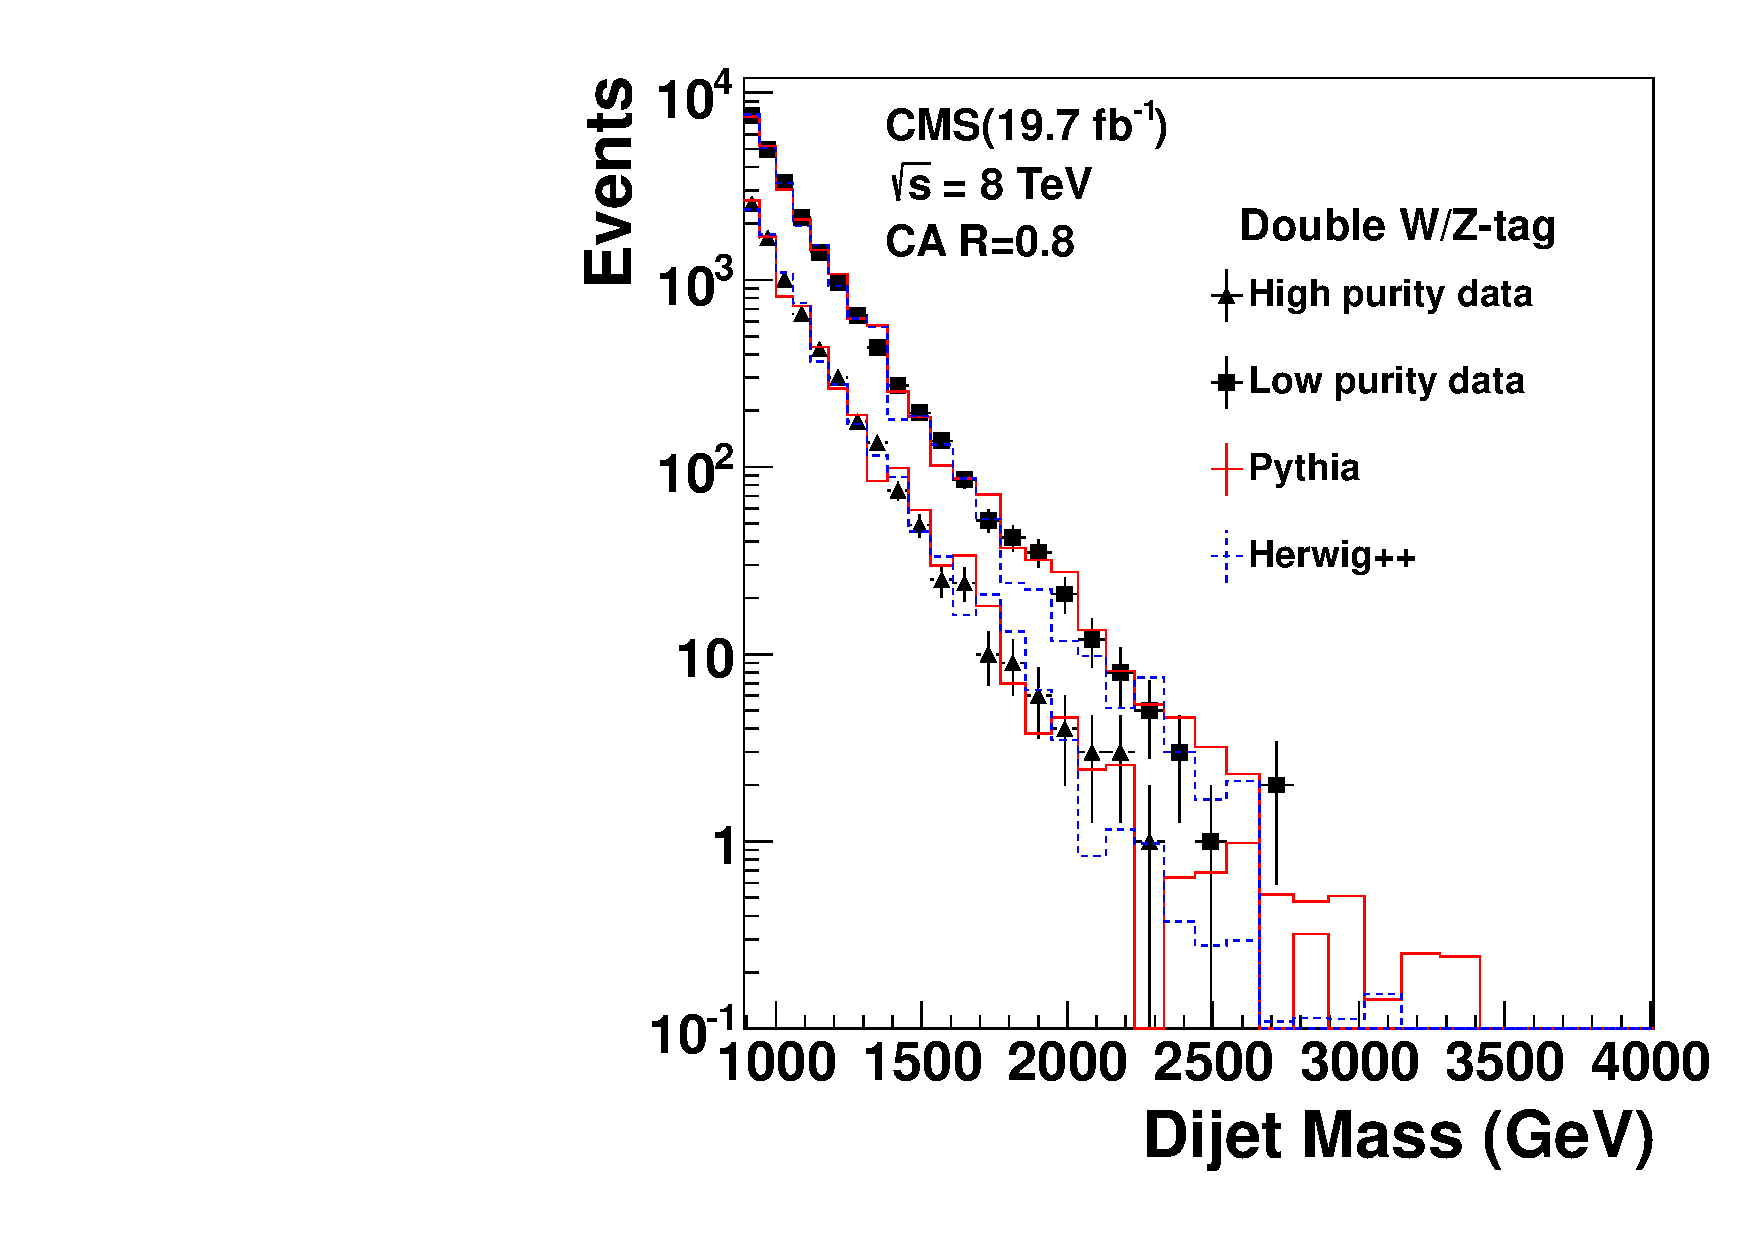
\includegraphics{figs/Data-MC-comparisons/DijetMass-VVMiumHigh.pdf}} \\
\end{tabular}
  \caption[Invariant Mass Double]{Comparisons between data and Monte Carlo
           for invariant mass of the two leading jets of low purity (left) and low-high purity (right) 2-tagged events.
           The MC is normalized to the number of data events in each category.
           }
  \label{fig:mjjDouble}
\end{figure}

\newpage
\begin{figure}[htb]
\centering
\begin{tabular}{cc}
     \resizebox{0.5\linewidth}{!}{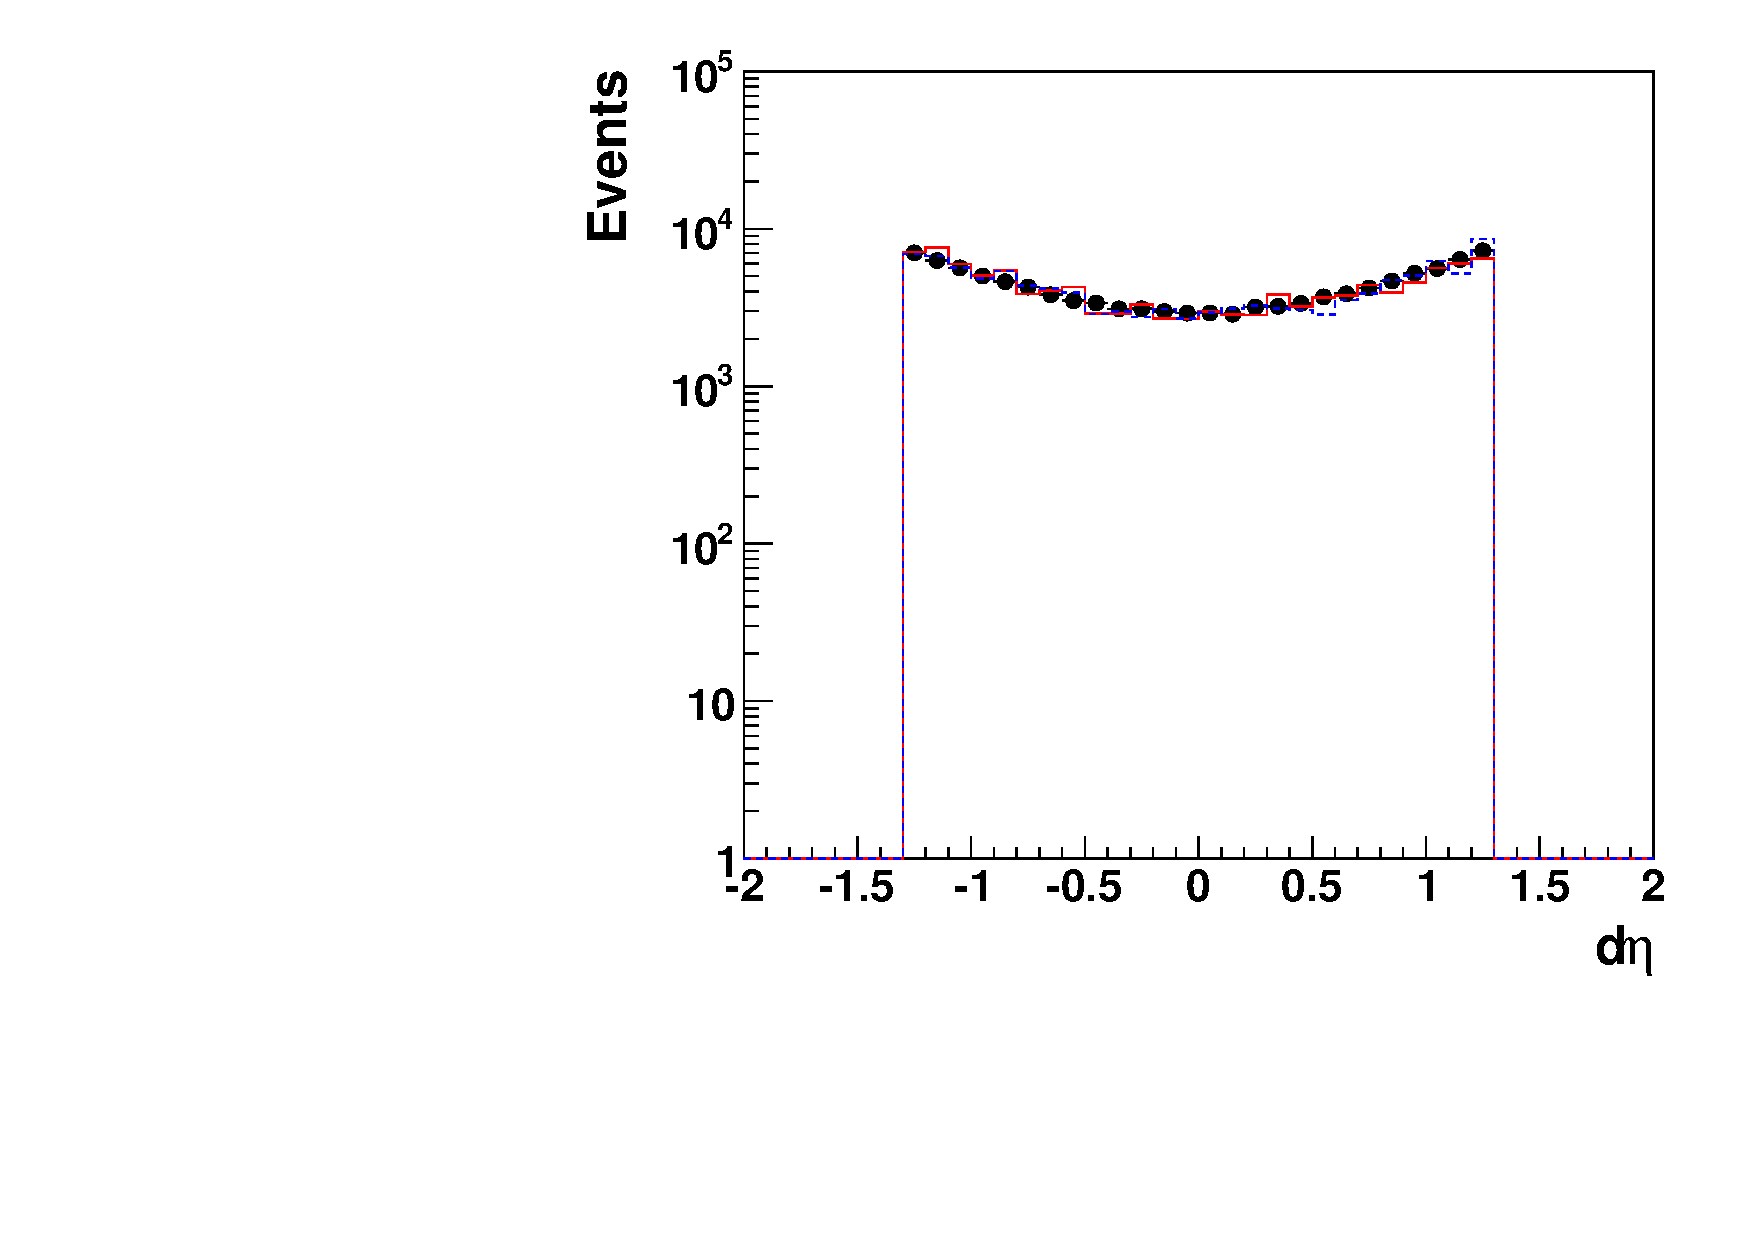
\includegraphics{figs/Data-MC-comparisons/Deta-qVLowP.pdf}} &
     \resizebox{0.5\linewidth}{!}{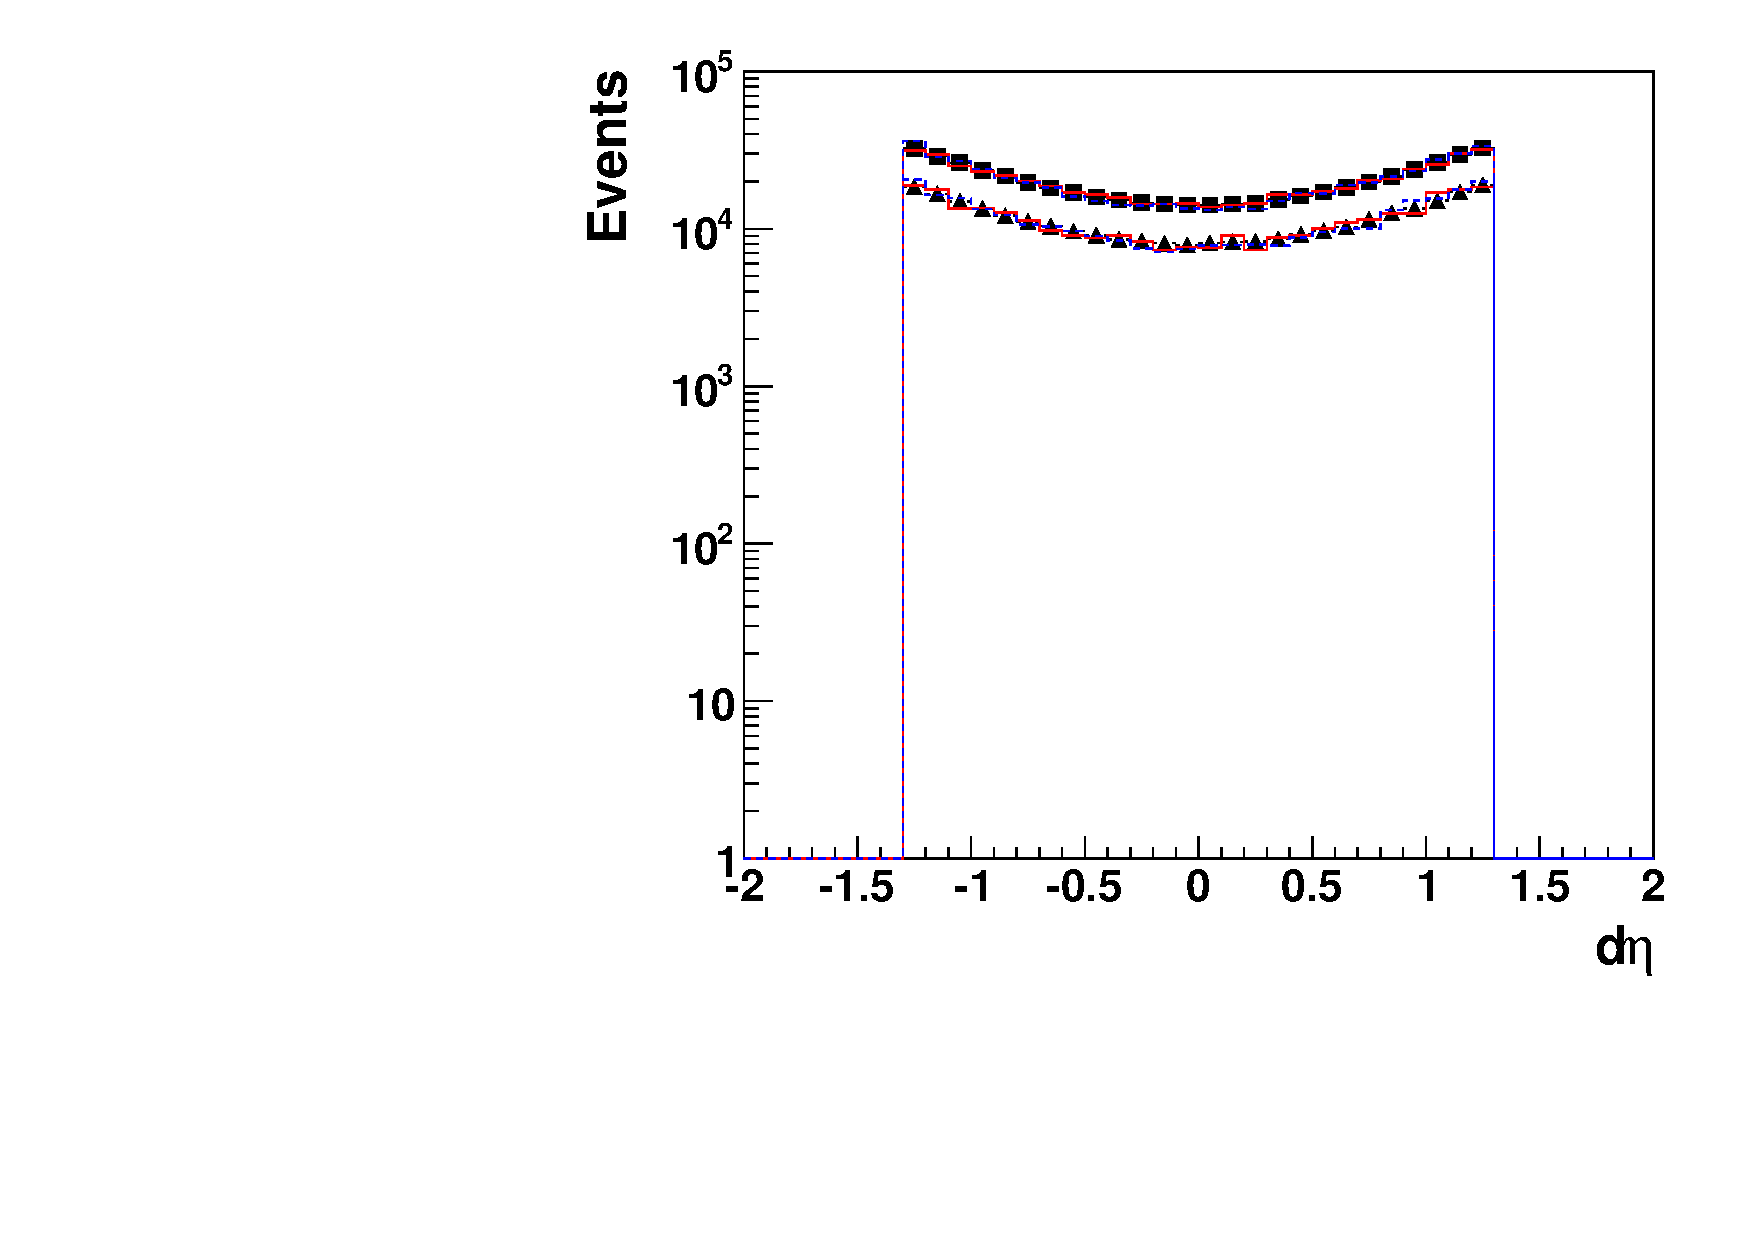
\includegraphics{figs/Data-MC-comparisons/Deta-qVMiumHigh.pdf}} \\
\end{tabular}
  \caption[Delta Eta Single]{Comparisons between data and Monte Carlo
                    for $\Delta\eta$ of the two leading jets of low purity (left) and low-high purity (right) 1-tagged events.
	   The MC is normalized to the number of data events in each category. }
  \label{fig:dySingle}
\end{figure}

\begin{figure}[htb]
\centering
\begin{tabular}{cc}
     \resizebox{0.5\linewidth}{!}{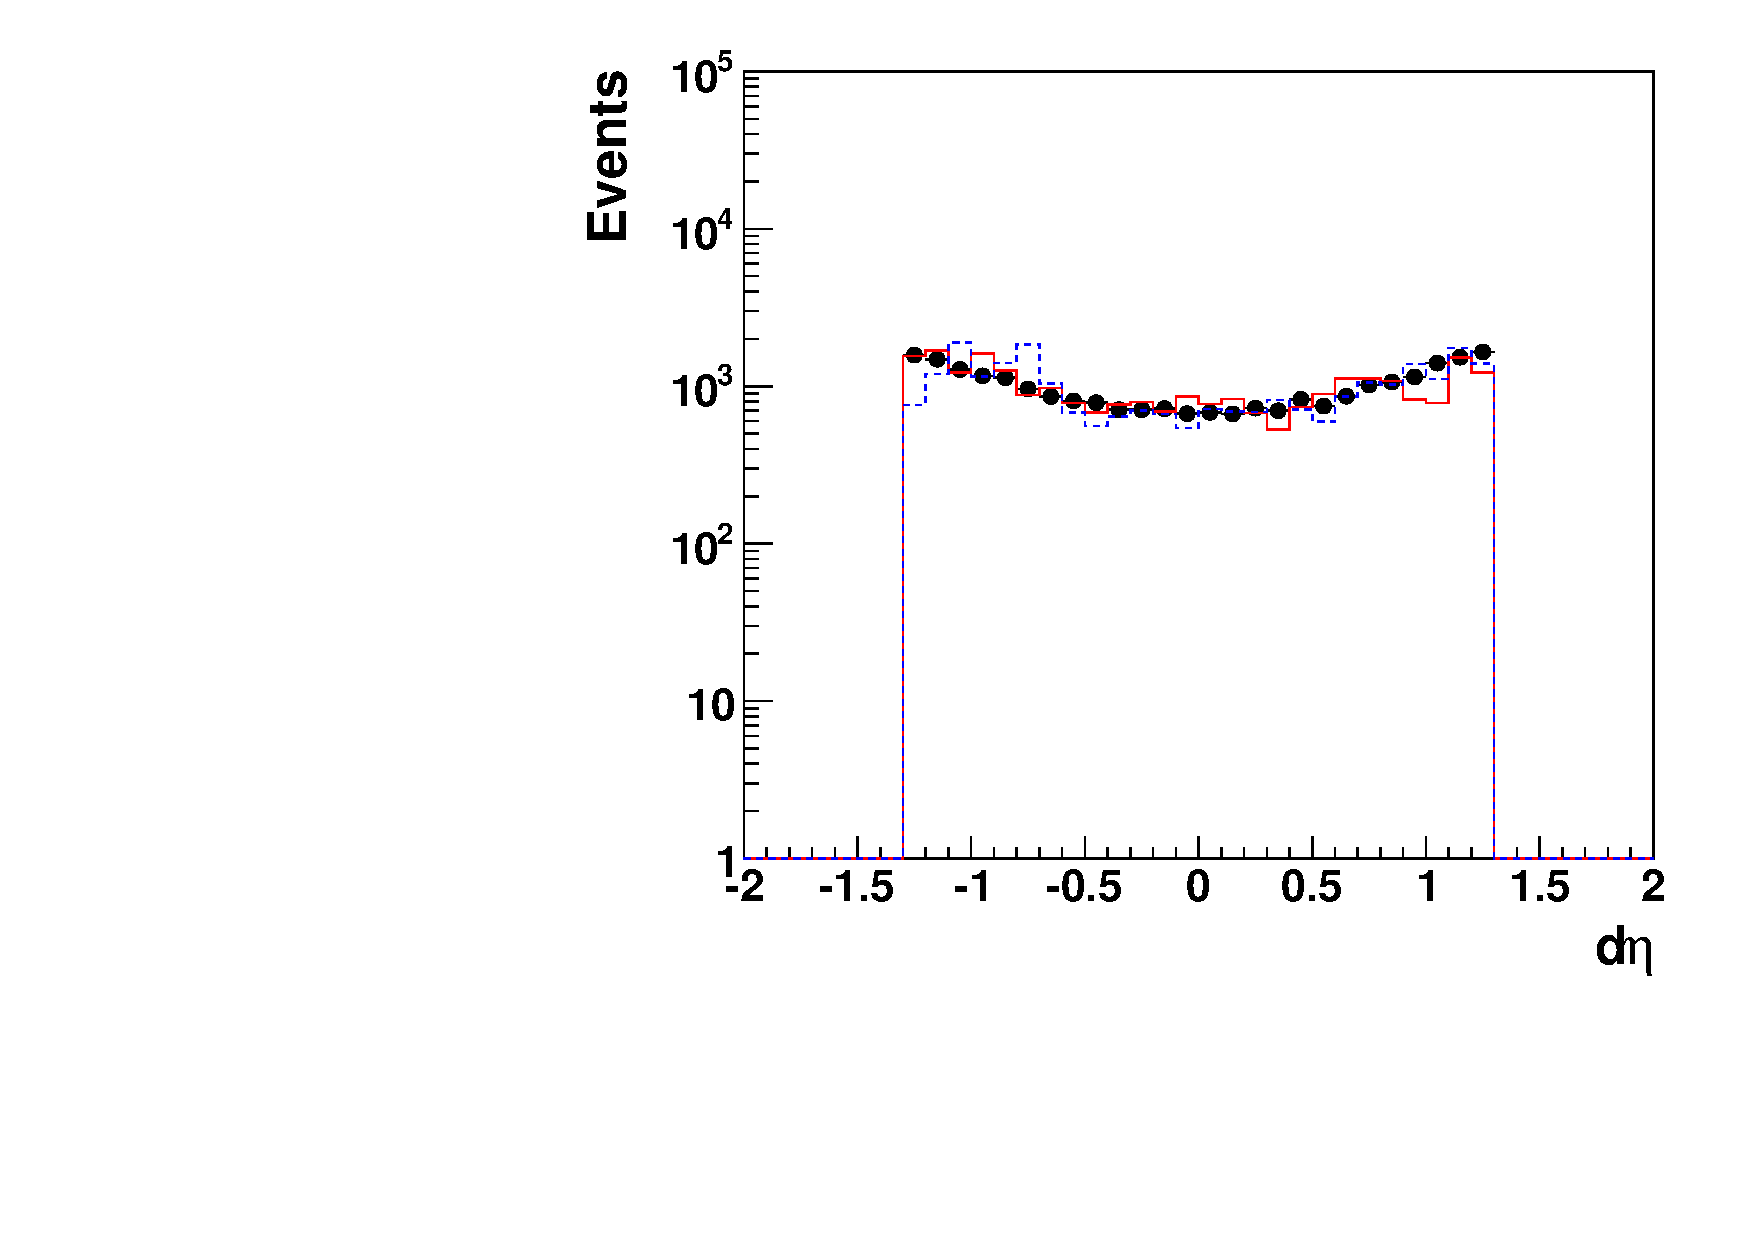
\includegraphics{figs/Data-MC-comparisons/Deta-VVLowP.pdf}} &
     \resizebox{0.5\linewidth}{!}{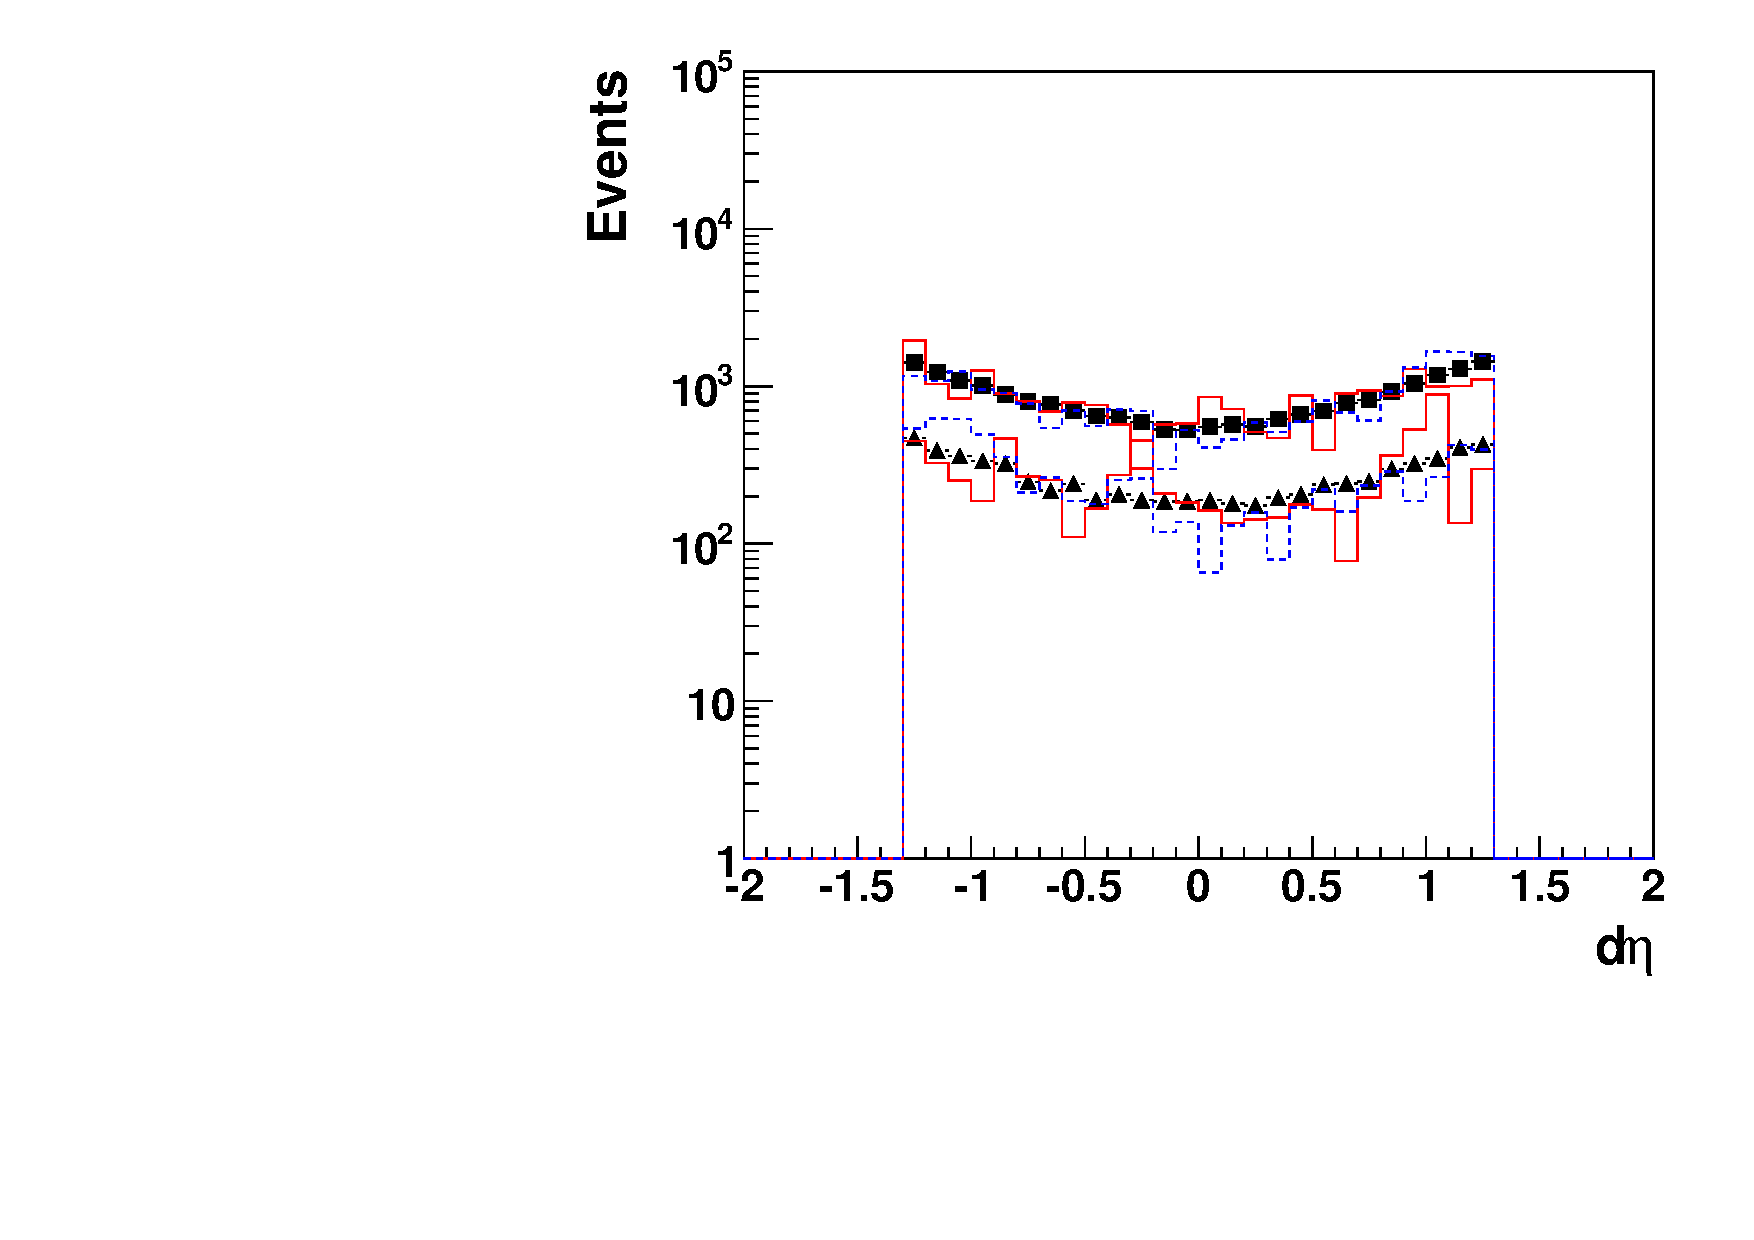
\includegraphics{figs/Data-MC-comparisons/Deta-VVMiumHigh.pdf}} \\
\end{tabular}
  \caption[Delta Eta Double]{Comparisons between data and Monte Carlo
                     for $\Delta\eta$ of the two leading jets of low purity (left) and low-high purity (right) 2-tagged events. The MC is normalized to the number of data events in each category. }
  \label{fig:dyDouble}
\end{figure}


\newpage
\begin{figure}[htb]
\centering
\begin{tabular}{cc}
     \resizebox{0.5\linewidth}{!}{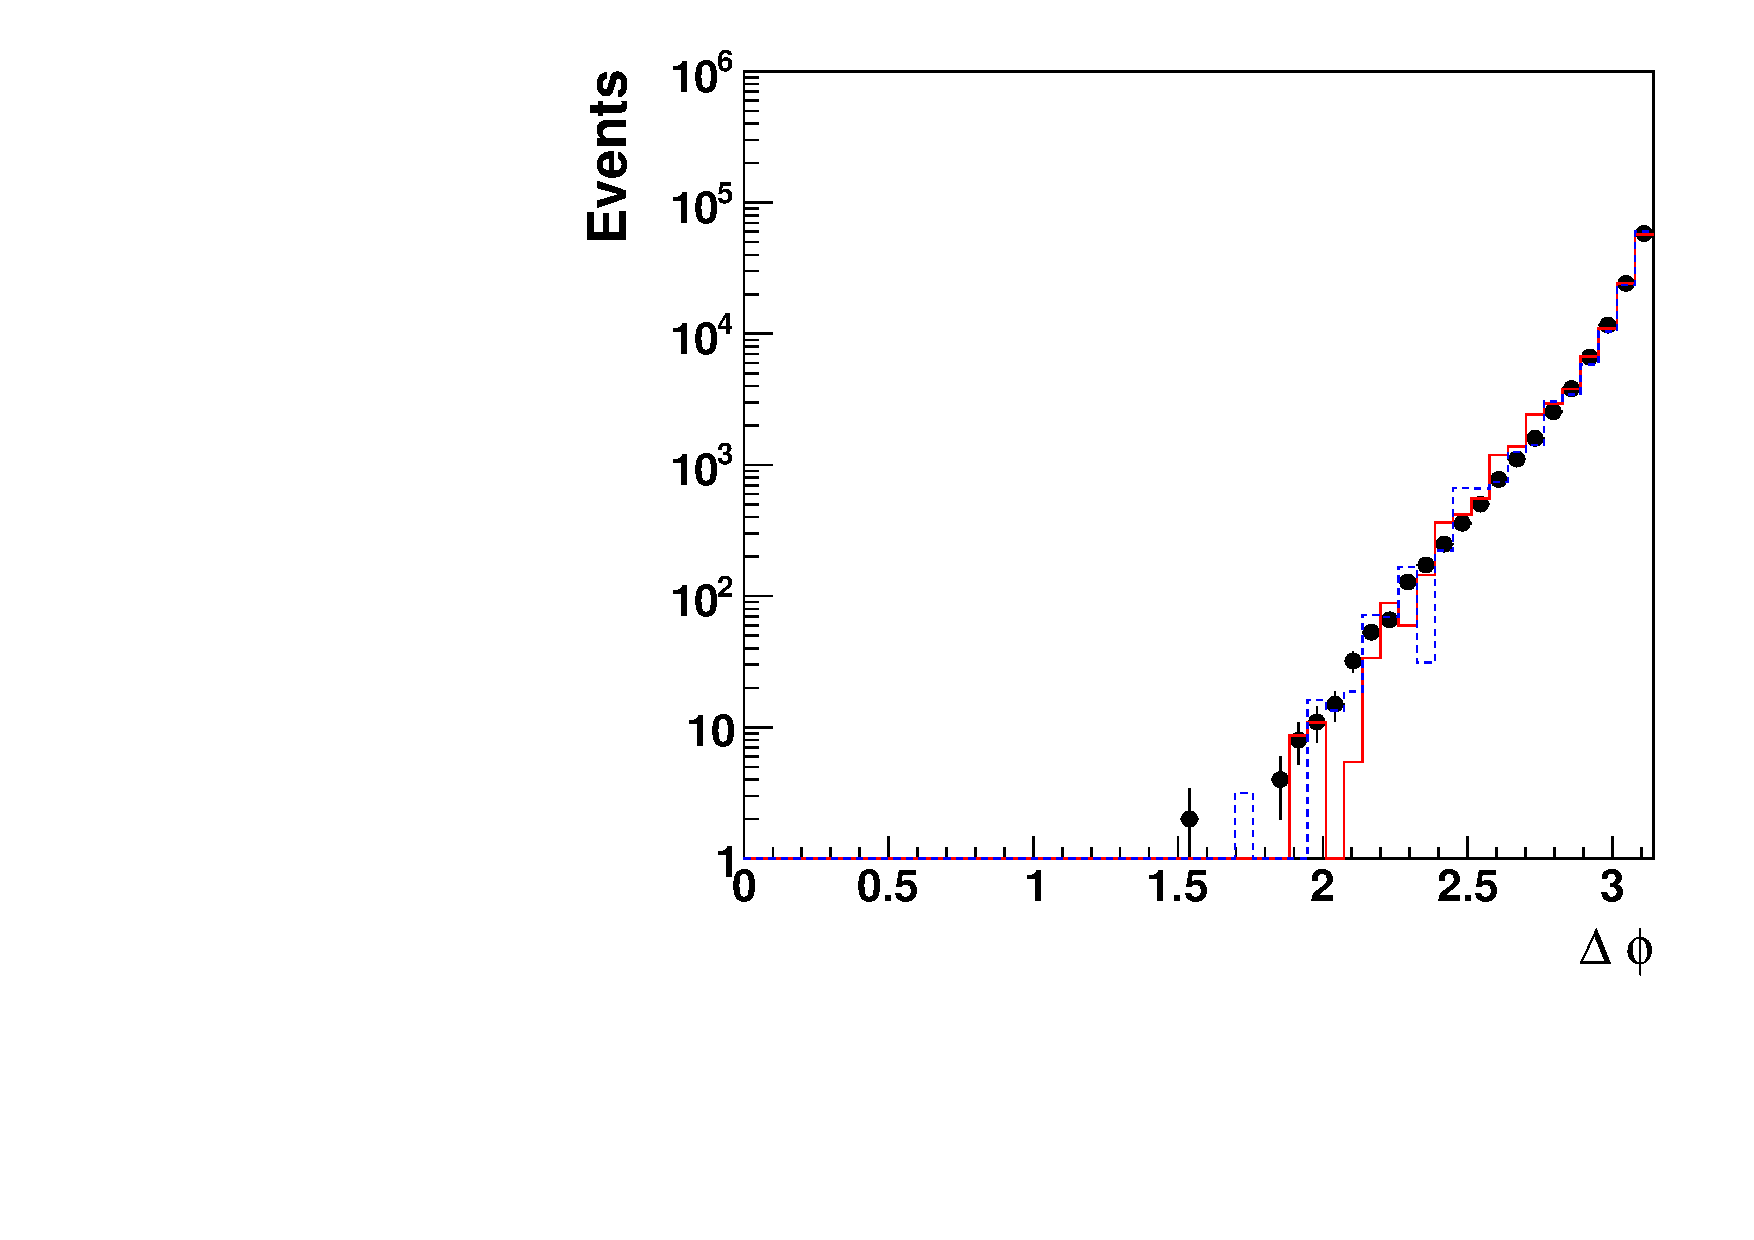
\includegraphics{figs/Data-MC-comparisons/Dphi-qVLowP.pdf}} &
     \resizebox{0.5\linewidth}{!}{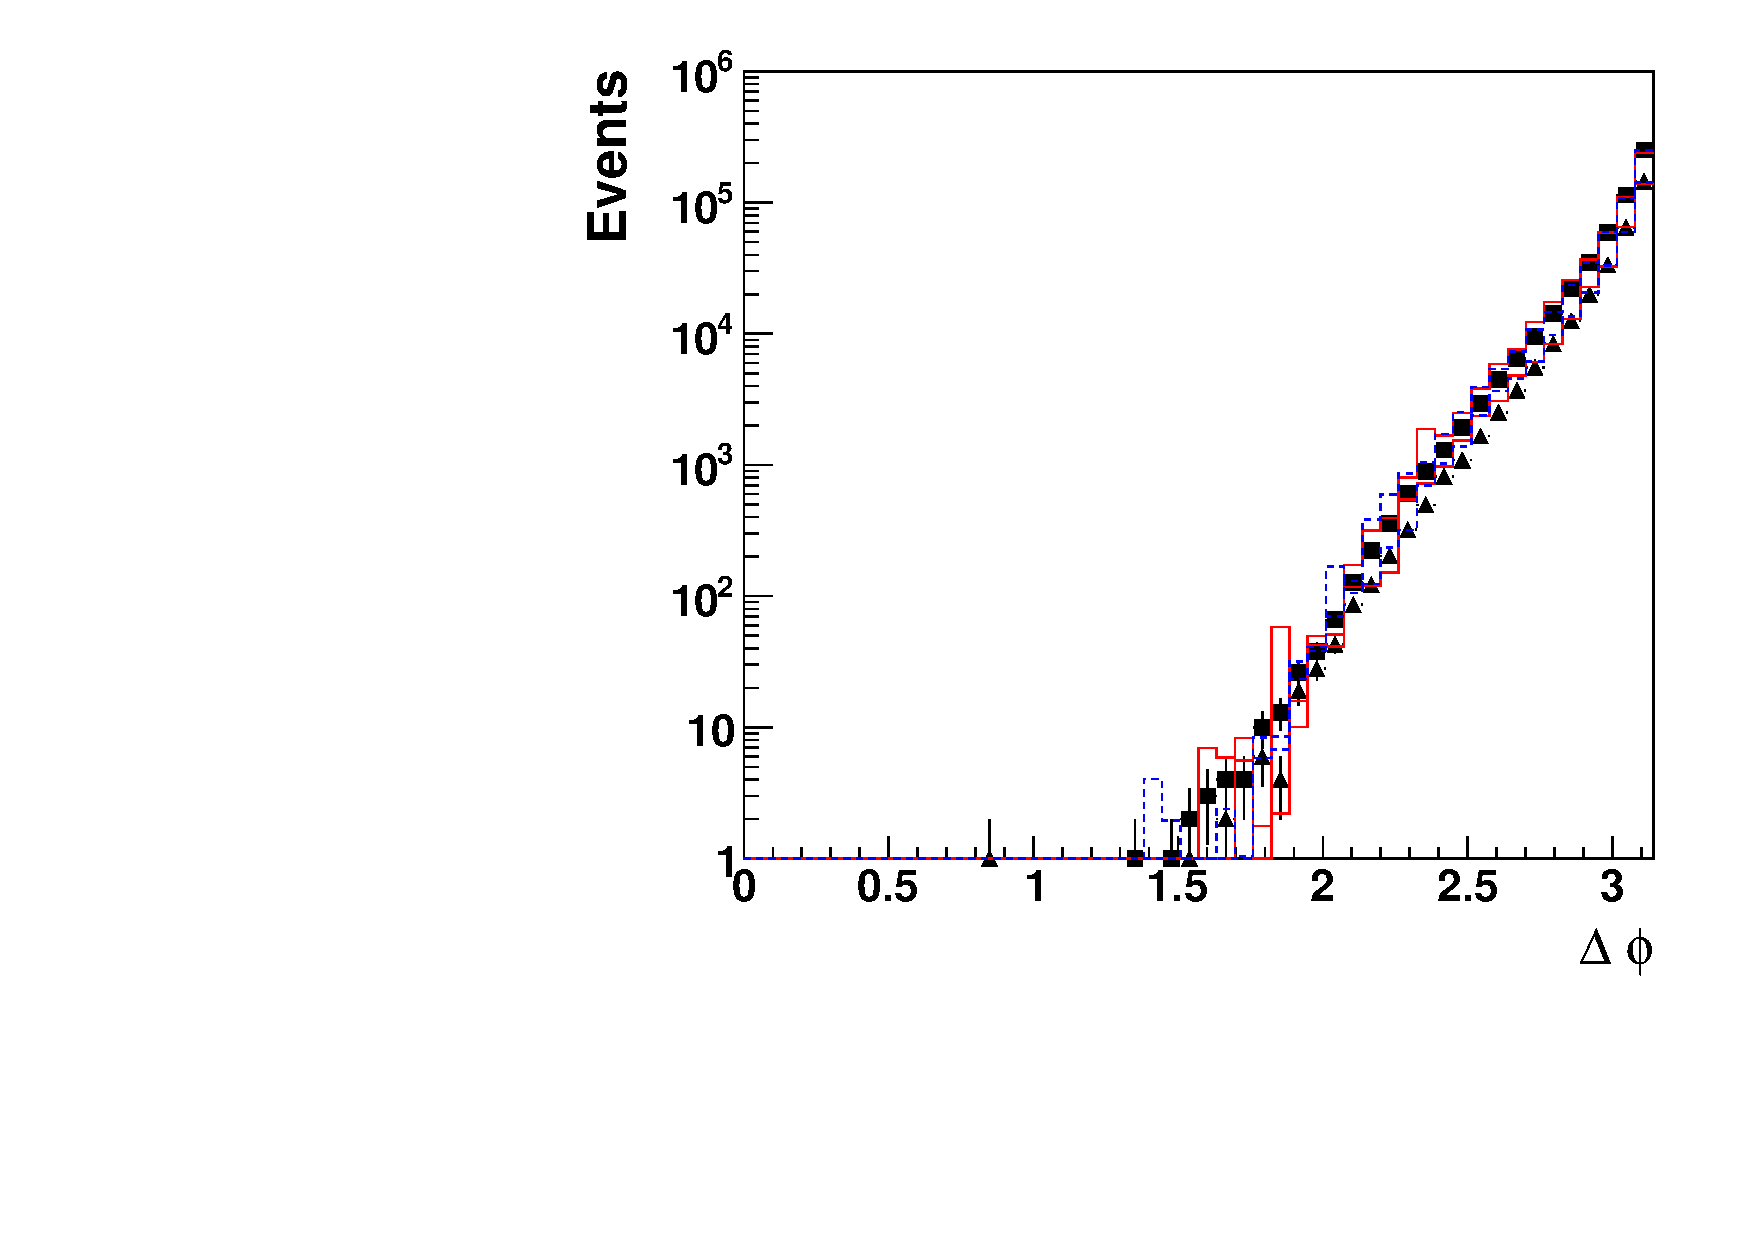
\includegraphics{figs/Data-MC-comparisons/Dphi-qVMiumHigh.pdf}} \\
\end{tabular}
  \caption[Delta Eta Single]{Comparisons between data and Monte Carlo
                    for $\Delta\phi$ of the two leading jets of low purity (left) and low-high purity (right) 1-tagged events.
	   The MC is normalized to the number of data events in each category. }
  \label{fig:dphiSingle}
\end{figure}

\begin{figure}[htb]
\centering
\begin{tabular}{cc}
     \resizebox{0.5\linewidth}{!}{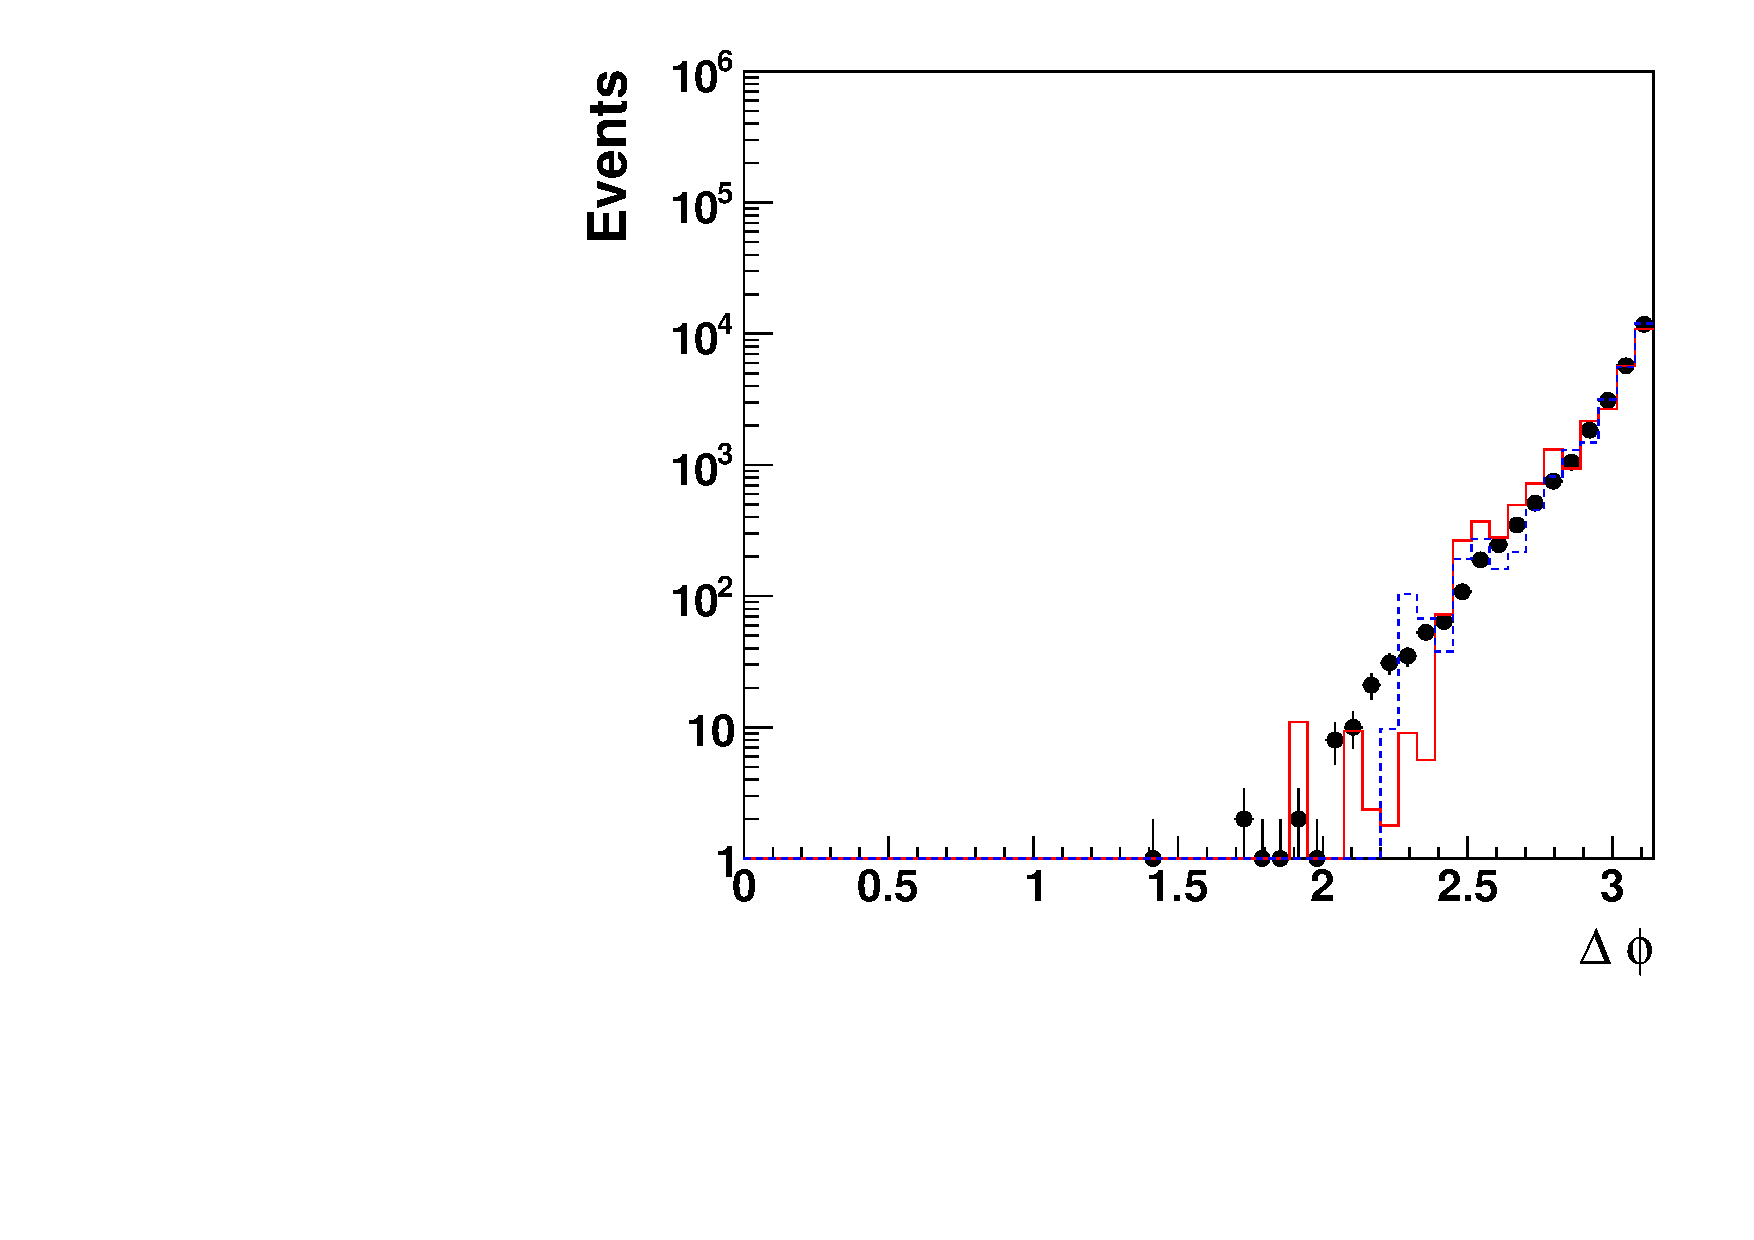
\includegraphics{figs/Data-MC-comparisons/Dphi-VVLowP.pdf}} &
     \resizebox{0.5\linewidth}{!}{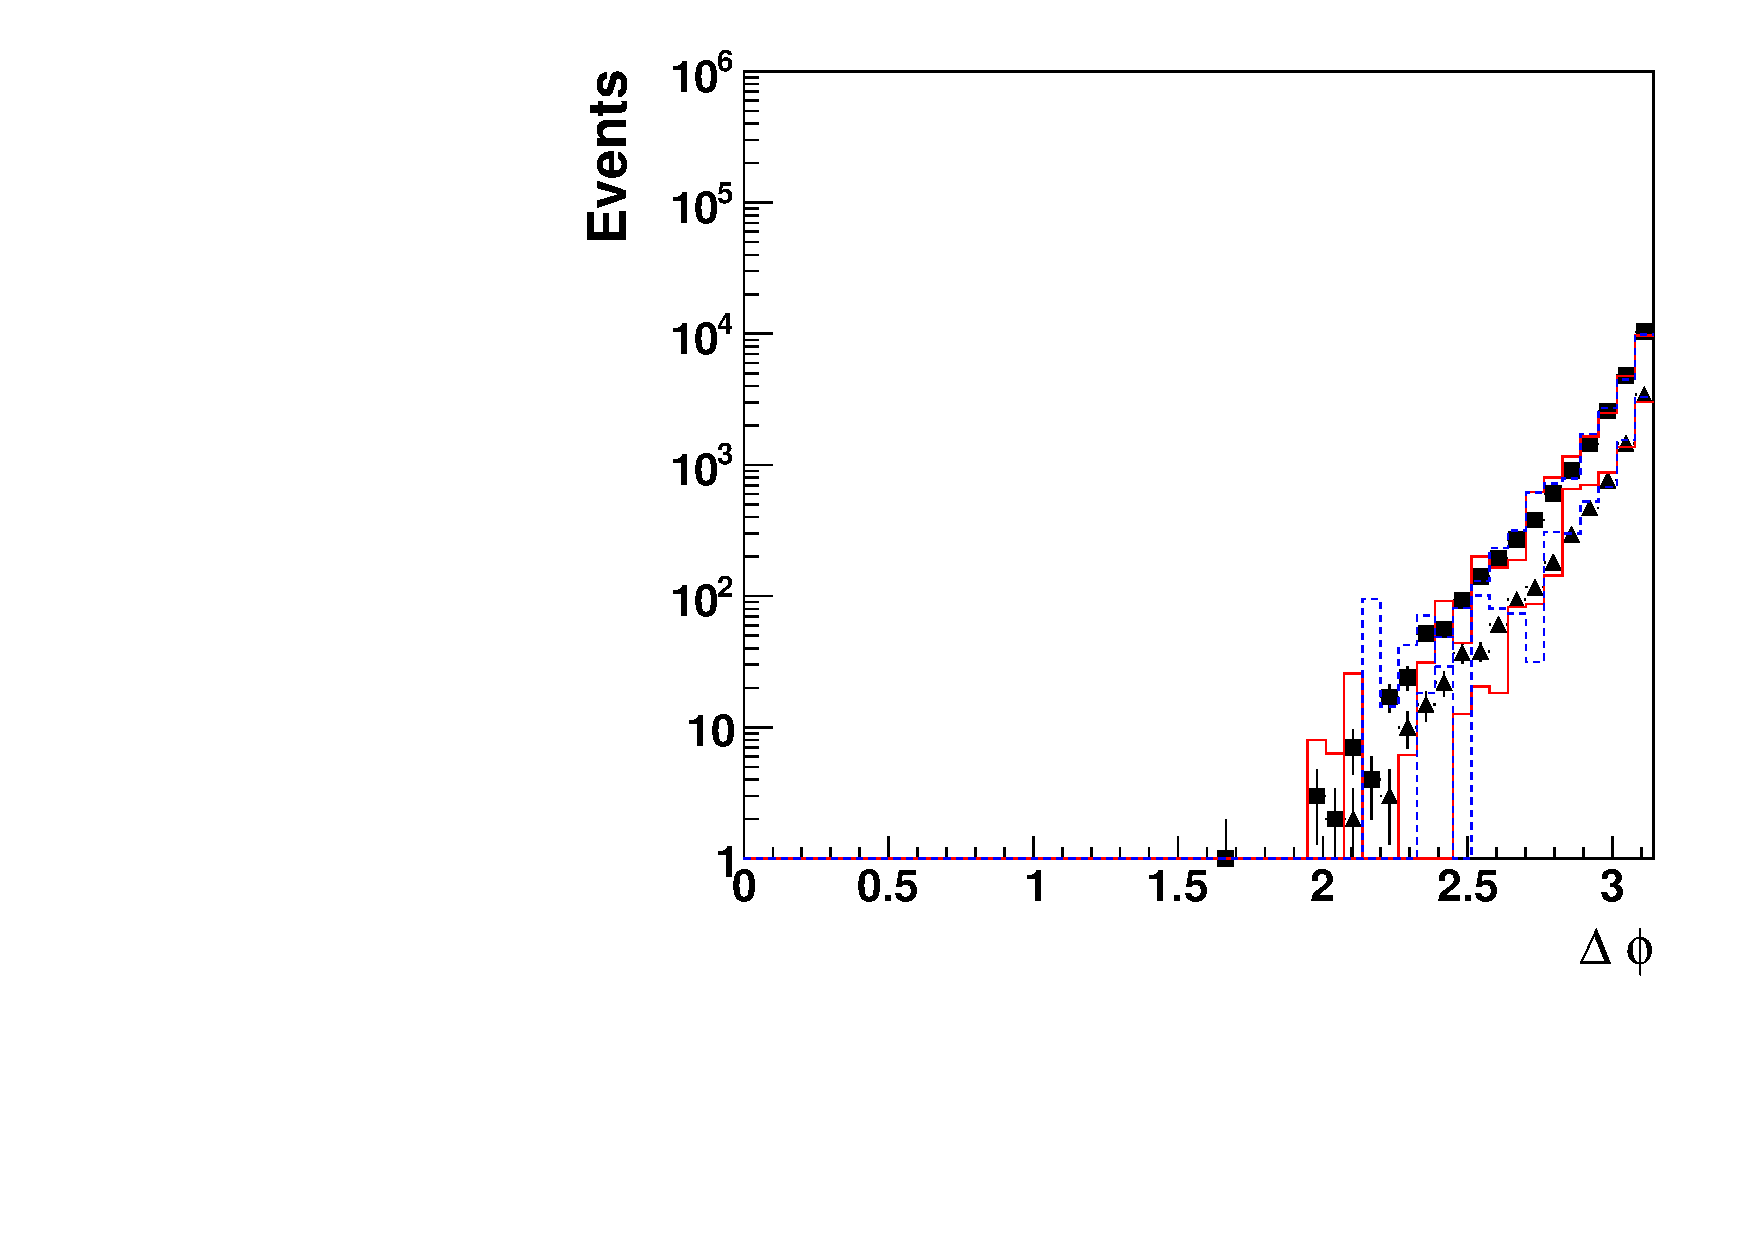
\includegraphics{figs/Data-MC-comparisons/Dphi-VVMiumHigh.pdf}} \\
\end{tabular}
  \caption[Delta Eta Double]{Comparisons between data and Monte Carlo
                     for $\Delta\phi$ of the two leading jets of low purity (left) and low-high purity (right) 2-tagged events. The MC is normalized to the number of data events in each category. }
  \label{fig:dphiDouble}
\end{figure}

\newpage

\begin{figure}[htb]
\centering
\begin{tabular}{cc}
     \resizebox{0.5\linewidth}{!}{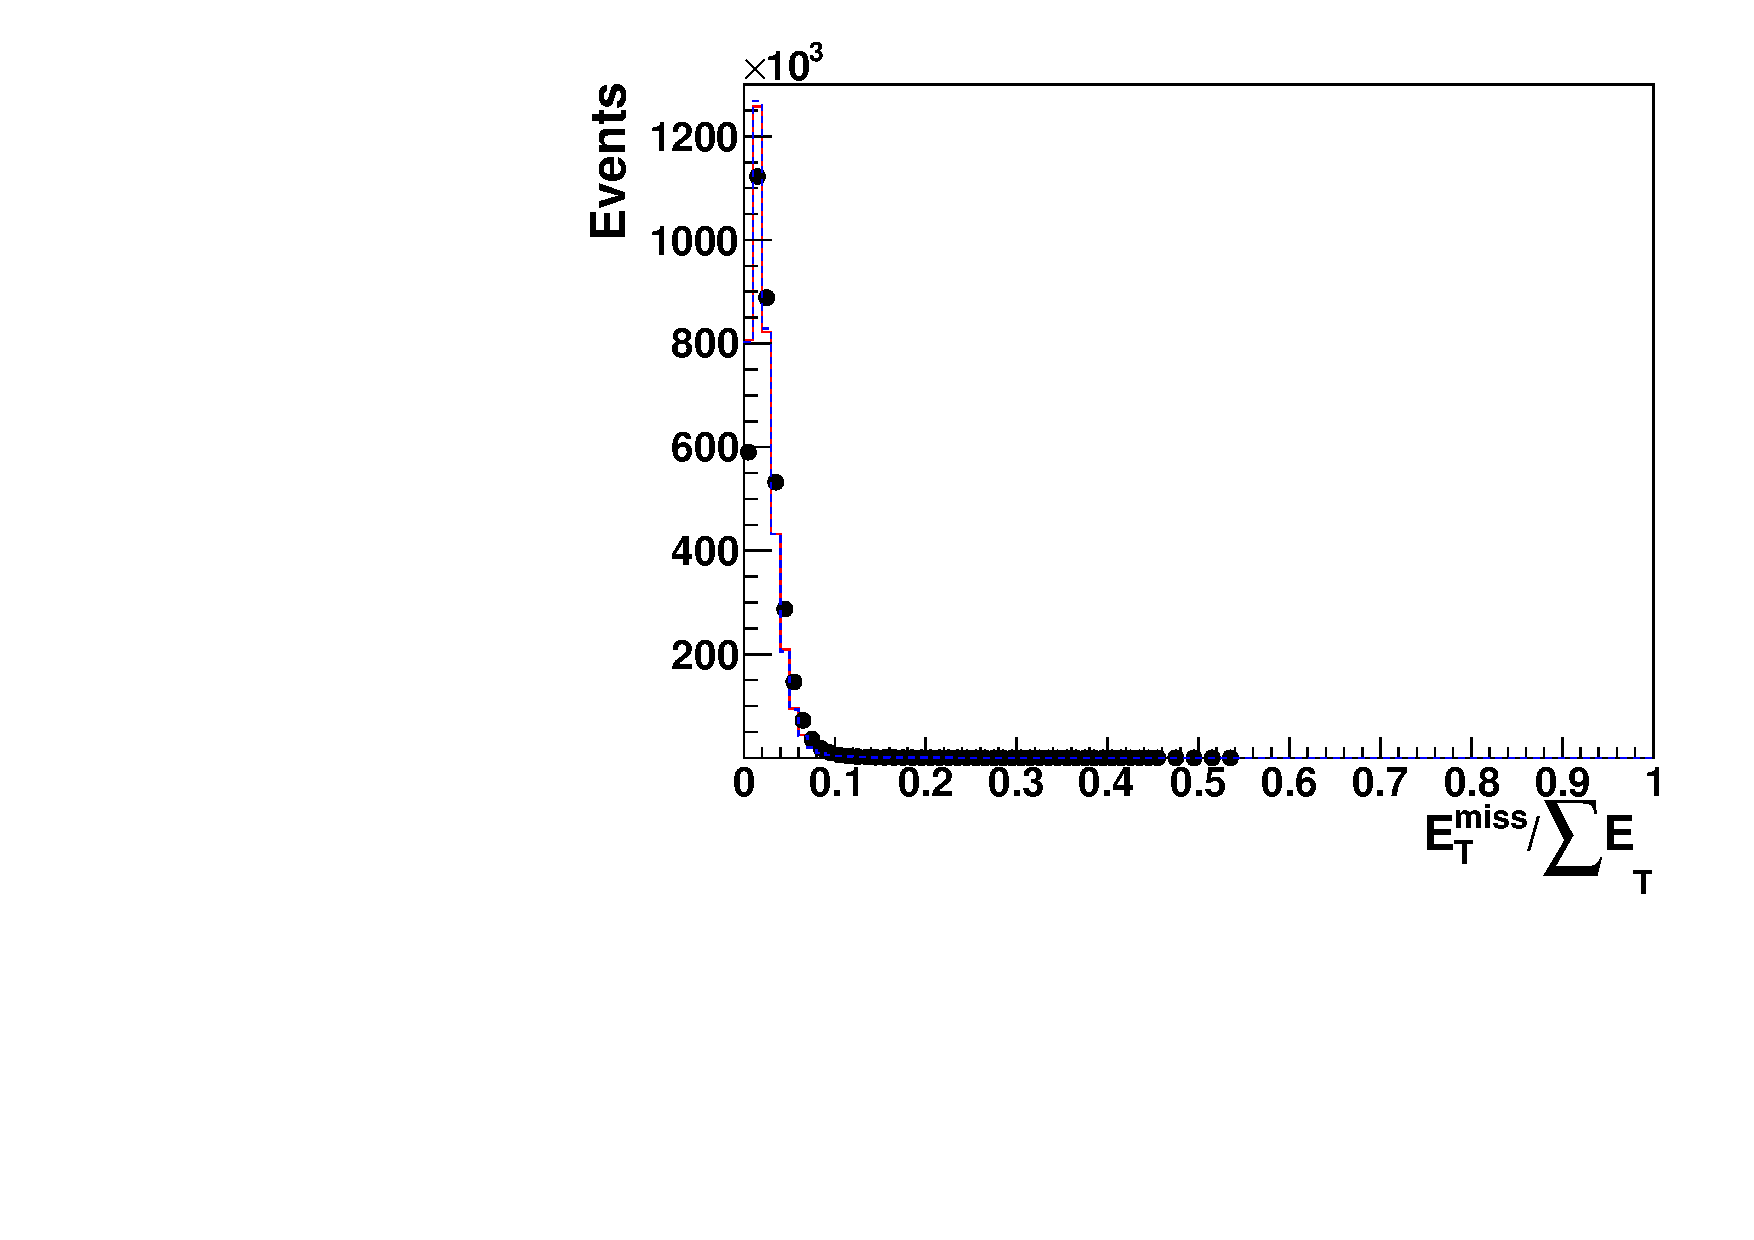
\includegraphics{figs/Data-MC-comparisons/etsumEt.pdf}} &
     \resizebox{0.5\linewidth}{!}{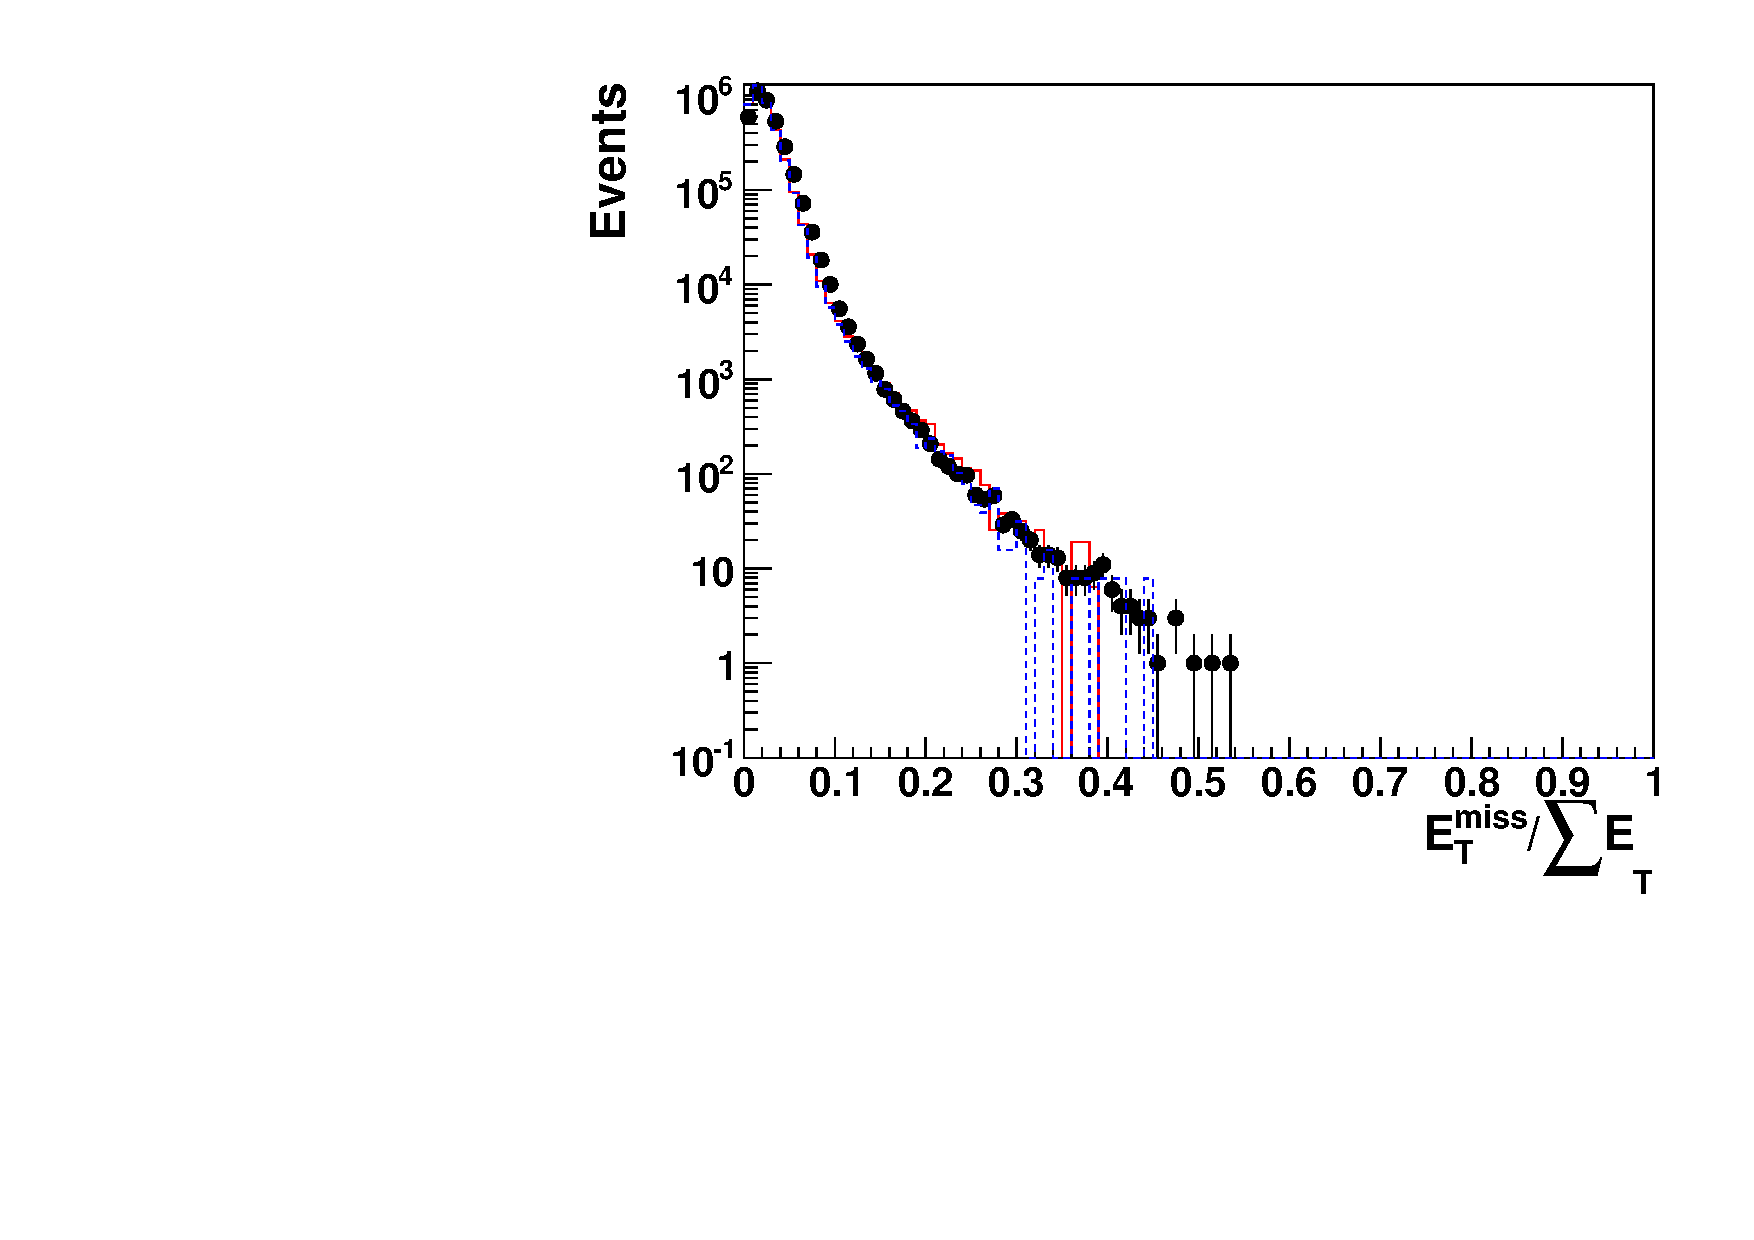
\includegraphics{figs/Data-MC-comparisons/etsumEtlog.pdf}} \\
\end{tabular}
  \caption[Leading two jets mass drop]{Comparisons between data and Monte Carlo for $E_{T}^{miss}/\sum E_{T}$ 
	   The MC is normalized to the number of data events. Plot on the right is the log scale plot. (The plot includes only a subset of the full data sample.)}
  \label{fig:metSumPtSingle}
\end{figure}

%\begin{figure}[htb]
%\centering
%\begin{tabular}{cc}
%     \resizebox{0.5\linewidth}{!}{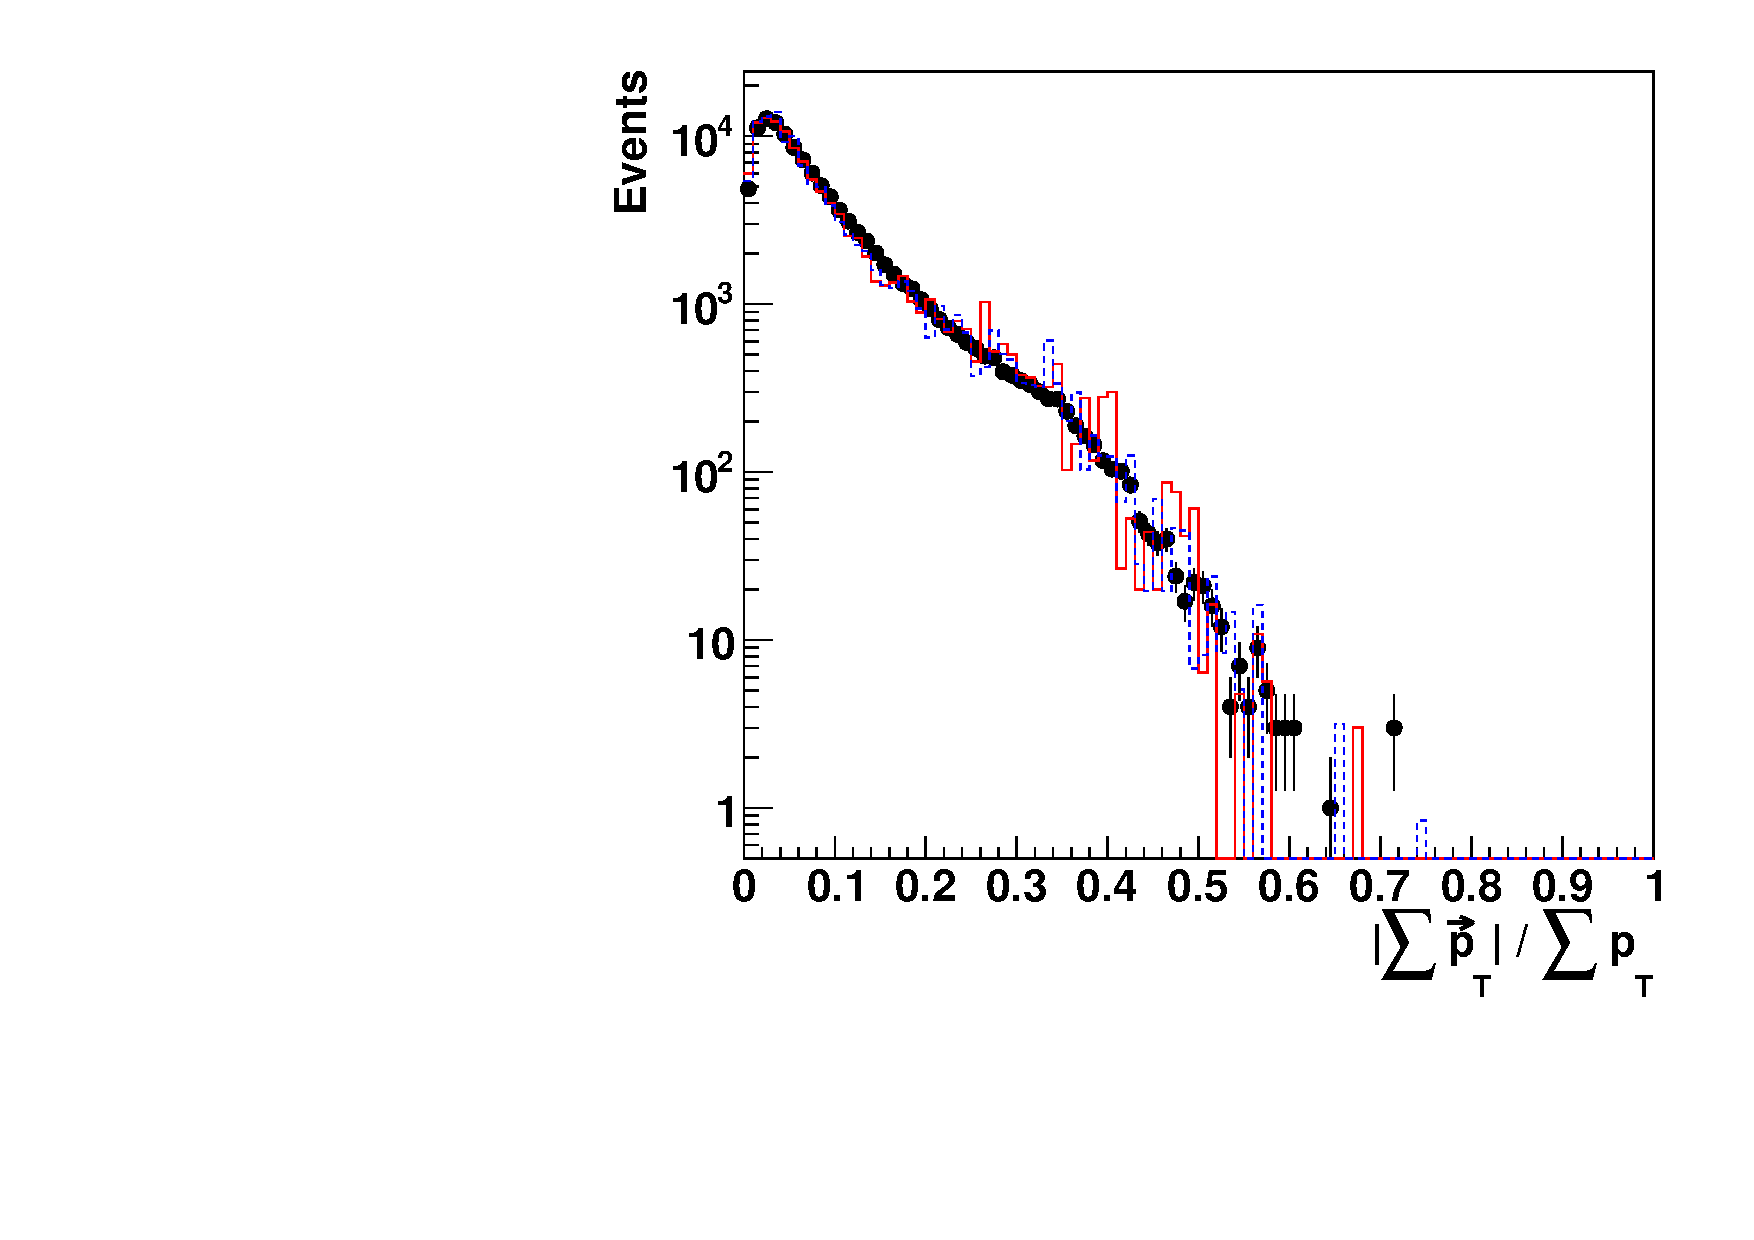
\includegraphics{figs/Data-MC-comparisons/PTVSPT-qVLowP.pdf}} &
%     \resizebox{0.5\linewidth}{!}{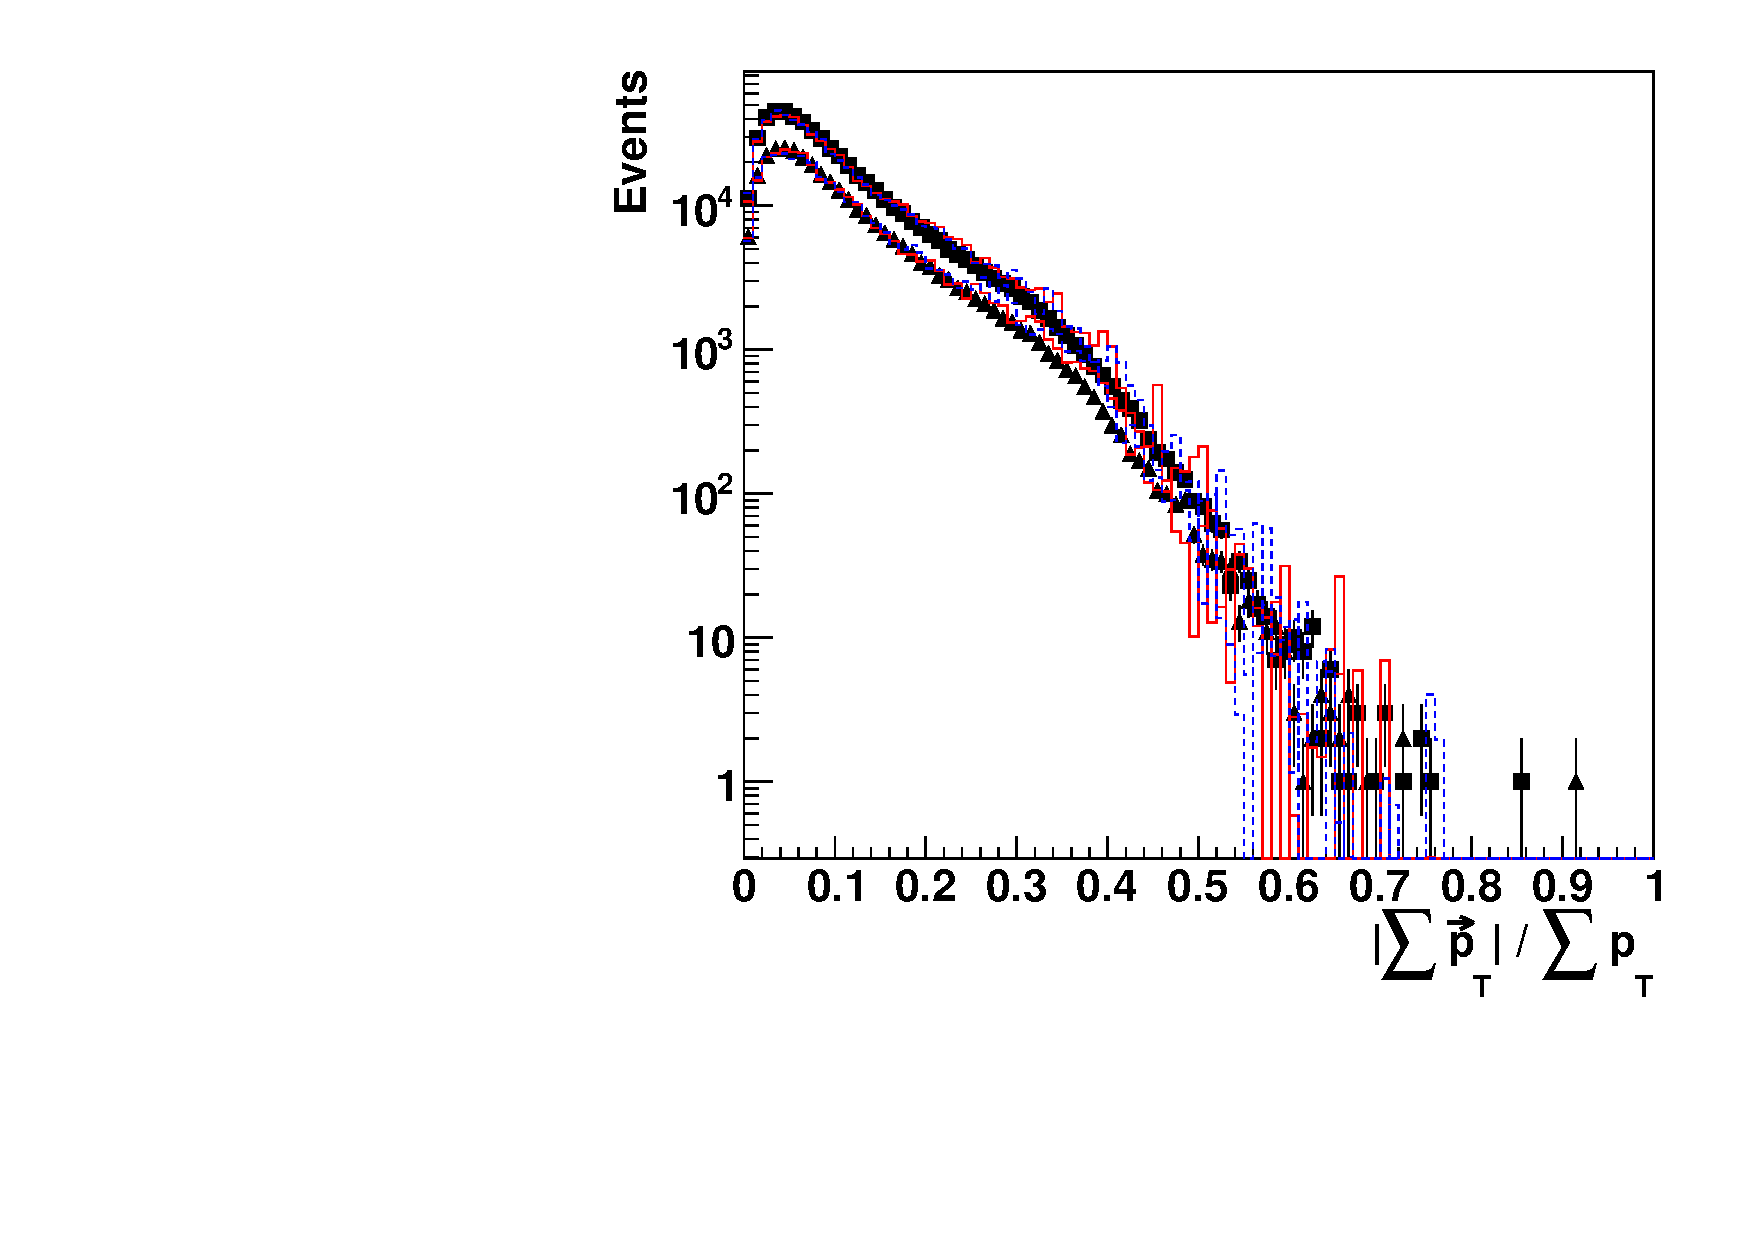
\includegraphics{figs/Data-MC-comparisons/PTVSPT-qVMiumHigh.pdf}} \\
%\end{tabular}
%  \caption[Delta Eta Single]{Comparisons between data and Monte Carlo
%                    for $|\sum{\vec{p}_{T}}| / \sum{p_{T}}$ of the two leading jets of low purity (left) and low-high purity (right) 1-tagged events.
%	   The MC is normalized to the number of data events in each category. }
%  \label{fig:metSumPtSingle}
%\end{figure}

%\begin{figure}[htb]
%\centering
%\begin{tabular}{cc}
%     \resizebox{0.5\linewidth}{!}{\includegraphics{figs/Data-MC-comparisons/PTVSPT-VVLowP.pdf}} &
%     \resizebox{0.5\linewidth}{!}{\includegraphics{figs/Data-MC-comparisons/PTVSPT-VVMiumHigh.pdf}} \\
%\end{tabular}
%  \caption[Delta Eta Double]{Comparisons between data and Monte Carlo
%                     for $|\sum{\vec{p}_{T}}| / \sum{p_{T}}$ of the two leading jets of low purity (left) and low-high purity (right) 2-tagged events. The MC is normalized to the number of data events in each category. }
%  \label{fig:metSumPtDouble}
%\end{figure}

\newpage
\begin{figure}[htb]
\centering
\begin{tabular}{cc}
     \resizebox{0.5\linewidth}{!}{\includegraphics{figs/Data-MC-comparisons/PT0-qVLowP.pdf}} &
     \resizebox{0.5\linewidth}{!}{\includegraphics{figs/Data-MC-comparisons/PT0-qVMiumHigh.pdf}} \\
\end{tabular}
  \caption[PT Single]{Comparisons between data and Monte Carlo
                    for $\pt$ of the leading jet of low purity (left) and low-high purity (right) 1-tagged events.
	   The MC is normalized to the number of data events in each category. }
  \label{fig:Pt0Single}
\end{figure}

\begin{figure}[htb]
\centering
\begin{tabular}{cc}
     \resizebox{0.5\linewidth}{!}{\includegraphics{figs/Data-MC-comparisons/PT0-VVLowP.pdf}} &
     \resizebox{0.5\linewidth}{!}{\includegraphics{figs/Data-MC-comparisons/PT0-VVMiumHigh.pdf}} \\
\end{tabular}
  \caption[Delta Eta Double]{Comparisons between data and Monte Carlo
                     for $\pt$ of the leading jet of low purity (left) and low-high purity (right) 2-tagged events. The MC is normalized to the number of data events in each category. }
  \label{fig:Pt0Double}
\end{figure}

\newpage
\begin{figure}[htb]
\centering
\begin{tabular}{cc}
     \resizebox{0.5\linewidth}{!}{\includegraphics{figs/Data-MC-comparisons/PT1-qVLowP.pdf}} &
     \resizebox{0.5\linewidth}{!}{\includegraphics{figs/Data-MC-comparisons/PT1-qVMiumHigh.pdf}} \\
\end{tabular}
  \caption[PT Single]{Comparisons between data and Monte Carlo
                    for $\pt$ of the second leading jet of low purity (left) and low-high purity (right) 1-tagged events.
	   The MC is normalized to the number of data events in each category. }
  \label{fig:Pt1Single}
\end{figure}

\begin{figure}[htb]
\centering
\begin{tabular}{cc}
     \resizebox{0.5\linewidth}{!}{\includegraphics{figs/Data-MC-comparisons/PT1-VVLowP.pdf}} &
     \resizebox{0.5\linewidth}{!}{\includegraphics{figs/Data-MC-comparisons/PT1-VVMiumHigh.pdf}} \\
\end{tabular}
  \caption[Delta Eta Double]{Comparisons between data and Monte Carlo
                     for $\pt$ of the second leading jet of low purity (left) and low-high purity (right) 2-tagged events. The MC is normalized to the number of data events in each category. }
  \label{fig:Pt1Double}
\end{figure}



\newpage
\begin{figure}[htb]
\centering
\begin{tabular}{cc}
     \resizebox{0.5\linewidth}{!}{\includegraphics{figs/Data-MC-comparisons/Eta0-qVLowP.pdf}} &
     \resizebox{0.5\linewidth}{!}{\includegraphics{figs/Data-MC-comparisons/Eta0-qVMiumHigh.pdf}} \\
\end{tabular}
  \caption[PT Single]{Comparisons between data and Monte Carlo
                    for $\eta$ of the leading jet of low purity (left) and low-high purity (right) 1-tagged events.
	   The MC is normalized to the number of data events in each category. }
  \label{fig:Eta0Single}
\end{figure}

\begin{figure}[htb]
\centering
\begin{tabular}{cc}
     \resizebox{0.5\linewidth}{!}{\includegraphics{figs/Data-MC-comparisons/Eta0-VVLowP.pdf}} &
     \resizebox{0.5\linewidth}{!}{\includegraphics{figs/Data-MC-comparisons/Eta0-VVMiumHigh.pdf}} \\
\end{tabular}
  \caption[Delta Eta Double]{Comparisons between data and Monte Carlo
                     for $\eta$ of the leading jet of low purity (left) and low-high purity (right) 2-tagged events. The MC is normalized to the number of data events in each category. }
  \label{fig:Eta0Double}
\end{figure}


\newpage
\begin{figure}[htb]
\centering
\begin{tabular}{cc}
     \resizebox{0.5\linewidth}{!}{\includegraphics{figs/Data-MC-comparisons/Eta1-qVLowP.pdf}} &
     \resizebox{0.5\linewidth}{!}{\includegraphics{figs/Data-MC-comparisons/Eta1-qVMiumHigh.pdf}} \\
\end{tabular}
  \caption[PT Single]{Comparisons between data and Monte Carlo
                    for $\eta$ of the second leading jet of low purity (left) and low-high purity (right) 1-tagged events.
	   The MC is normalized to the number of data events in each category. }
  \label{fig:Eta1Single}
\end{figure}

\begin{figure}[htb]
\centering
\begin{tabular}{cc}
     \resizebox{0.5\linewidth}{!}{\includegraphics{figs/Data-MC-comparisons/Eta1-VVLowP.pdf}} &
     \resizebox{0.5\linewidth}{!}{\includegraphics{figs/Data-MC-comparisons/Eta1-VVMiumHigh.pdf}} \\
\end{tabular}
  \caption[Delta Eta Double]{Comparisons between data and Monte Carlo
                     for $\eta$ of the second leading jet of low purity (left) and low-high purity (right) 2-tagged events. The MC is normalized to the number of data events in each category. }
  \label{fig:Eta1Double}
\end{figure}

%\newpage
%\begin{figure}[htb]
%\centering
%\begin{tabular}{cc}
%     \resizebox{0.5\linewidth}{!}{\includegraphics{figs/Data-MC-comparisons/CA8CA8-qVLowP.pdf}} &
%     \resizebox{0.5\linewidth}{!}{\includegraphics{figs/Data-MC-comparisons/CA8CA8-qVMiumHigh.pdf}} \\
%\end{tabular}
%  \caption[PT Single]{Comparisons between data and Monte Carlo
%                    for $\Delta \phi$ of the leading ungroomed CA8 jet and leading pruned CA8 jet of low purity (left) and low-high purity (right) 1-tagged events.
%	   The MC is normalized to the number of data events in each category. }
%  \label{fig:CA8Single}
%\end{figure}

%\begin{figure}[htb]
%\centering
%\begin{tabular}{cc}
%     \resizebox{0.5\linewidth}{!}{\includegraphics{figs/Data-MC-comparisons/CA8CA8-VVLowP.pdf}} &
%     \resizebox{0.5\linewidth}{!}{\includegraphics{figs/Data-MC-comparisons/CA8CA8-VVMiumHigh.pdf}} \\
%\end{tabular}
%  \caption[PT Single]{Comparisons between data and Monte Carlo
%                    for $\Delta \phi$ of the leading ungroomed CA8 jet and leading pruned CA8 jet of low purity (left) and low-high purity (right) 2-tagged events.
%           The MC is normalized to the number of data events in each category. }
%  \label{fig:CA8Double}
%\end{figure}


\newpage
\begin{figure}[htb]
\centering
\begin{tabular}{cc}
     \resizebox{0.5\linewidth}{!}{\includegraphics{figs/Data-MC-comparisons/lumi19fb_dataMC_ca8jet_norm_mlog.pdf}} &
     \resizebox{0.5\linewidth}{!}{\includegraphics{figs/Data-MC-comparisons/data-qcd-Jet-Tau21.pdf}}\\
\end{tabular}
  \caption[Leading two jets mass]{Comparisons between data and Monte Carlo for
                    mass(left) and $\tau_{21}$(right) of the leading two jets.
	   The MC is normalized to the number of data events in each category.}
  \label{fig:massNsub}
\end{figure}



















\newpage

\begin{figure}[htb]
\centering
\begin{tabular}{cc}
     \resizebox{0.5\linewidth}{!}{\includegraphics{figs/Data-MC-comparisons/npv.pdf}} &
     \resizebox{0.5\linewidth}{!}{\includegraphics{figs/Data-MC-comparisons/npvlog.pdf}} \\
\end{tabular}
  \caption[Leading two jets mass drop]{Comparisons between data and Monte Carlo for
                   number of primary vertice to show the effect on Monte Carlo after pile up reweighting. 
	   The MC is normalized to the number of data events. Plot on the right is the log scale plot. (The plot includes only a subset of the full data sample.)}
  \label{fig:npv}
\end{figure}

\begin{figure}[htb]
\centering
\begin{tabular}{cc}
     \resizebox{0.5\linewidth}{!}{\includegraphics{figs/Data-MC-comparisons/neutralHadronEnergyFraction.pdf}} &
     \resizebox{0.5\linewidth}{!}{\includegraphics{figs/Data-MC-comparisons/neutralHadronEnergyFractionlog.pdf}} \\
\end{tabular}
  \caption[Leading two jets mass drop]{Comparisons between data and Monte Carlo for neutral hadron energy fraction.  
	   The MC is normalized to the number of data events. Plot on the right is the log scale plot. (The plot includes only a subset of the full data sample.)}
  \label{fig:neutralHadronEnergyFraction}
\end{figure}

\newpage

\begin{figure}[htb]
\centering
\begin{tabular}{cc}
     \resizebox{0.5\linewidth}{!}{\includegraphics{figs/Data-MC-comparisons/neutralEmEnergyFraction.pdf}} &
     \resizebox{0.5\linewidth}{!}{\includegraphics{figs/Data-MC-comparisons/neutralEmEnergyFractionlog.pdf}} \\
\end{tabular}
  \caption[Leading two jets mass drop]{Comparisons between data and Monte Carlo for neutral eletromagnetic energy fraction.  
	   The MC is normalized to the number of data events. Plot on the right is the log scale plot. (The plot includes only a subset of the full data sample.)}
  \label{fig:neutralEmEnergyFraction}
\end{figure}

\begin{figure}[htb]
\centering
\begin{tabular}{cc}
     \resizebox{0.5\linewidth}{!}{\includegraphics{figs/Data-MC-comparisons/chargedHadronEnergyFraction.pdf}} &
     \resizebox{0.5\linewidth}{!}{\includegraphics{figs/Data-MC-comparisons/chargedHadronEnergyFractionlog.pdf}} \\
\end{tabular}
  \caption[Leading two jets mass drop]{Comparisons between data and Monte Carlo for charged hadron energy fraction.  
	   The MC is normalized to the number of data events. Plot on the right is the log scale plot. (The plot includes only a subset of the full data sample.)}
  \label{fig:chargedHadronEnergyFraction}
\end{figure}

\newpage


\begin{figure}[htb]
\centering
\begin{tabular}{cc}
     \resizebox{0.5\linewidth}{!}{\includegraphics{figs/Data-MC-comparisons/chargedEmEnergyFraction.pdf}} &
     \resizebox{0.5\linewidth}{!}{\includegraphics{figs/Data-MC-comparisons/chargedEmEnergyFractionlog.pdf}} \\
\end{tabular}
  \caption[Leading two jets mass drop]{Comparisons between data and Monte Carlo for charged eletromagnetic energy fraction.  
	   The MC is normalized to the number of data events. Plot on the right is the log scale plot. (The plot includes only a subset of the full data sample.)}
  \label{fig:chargedEmEnergyFraction}
\end{figure}

\begin{figure}[htb]
\centering
\begin{tabular}{cc}
     \resizebox{0.5\linewidth}{!}{\includegraphics{figs/Data-MC-comparisons/chargedMultiplicity.pdf}} &
     \resizebox{0.5\linewidth}{!}{\includegraphics{figs/Data-MC-comparisons/chargedMultiplicitylog.pdf}} \\
\end{tabular}
  \caption[Leading two jets mass drop]{Comparisons between data and Monte Carlo for charged multiplicity.  
	   The MC is normalized to the number of data events. Plot on the right is the log scale plot. (The plot includes only a subset of the full data sample.)}
  \label{fig:chargedMultiplicity}
\end{figure}

\newpage

\begin{figure}[htb]
\centering
\begin{tabular}{cc}
     \resizebox{0.5\linewidth}{!}{\includegraphics{figs/Data-MC-comparisons/nConstituents.pdf}} &
     \resizebox{0.5\linewidth}{!}{\includegraphics{figs/Data-MC-comparisons/nConstituentslog.pdf}} \\
\end{tabular}
  \caption[Leading two jets mass drop]{Comparisons between data and Monte Carlo for number of constituents.  
	   The MC is normalized to the number of data events. Plot on the right is the log scale plot. (The plot includes only a subset of the full data sample.)}
  \label{fig:nConstituents}
\end{figure}


\begin{figure}[htb]
\centering
\begin{tabular}{cc}
     \resizebox{0.5\linewidth}{!}{\includegraphics{figs/Data-MC-comparisons/muonEnergyFraction.pdf}} &
     \resizebox{0.5\linewidth}{!}{\includegraphics{figs/Data-MC-comparisons/muonEnergyFractionlog.pdf}} \\
\end{tabular}
  \caption[Leading two jets mass drop]{Comparisons between data and Monte Carlo for the muon energy fraction of the leading two jets.  
	   The MC is normalized to the number of data events. Plot on the right is the log scale plot. (The plot includes only a subset of the full data sample.)}
  \label{fig:muonEnergyFraction}
\end{figure}

\newpage


%We find that the QCD MC agrees with data, although not perfect.
%For the dijet kinematics shown in Fig~\ref{fig:mjj},\ref{fig:dy},\ref{fig:dphi},\ref{fig:metSumPt},\ref{fig:jet1-pt},\ref{fig:jet2-pt},\ref{fig:eta of leading jet} and \ref{fig:eta of second leading jet}, we observe better agreement of Pythia6 $Z2*$ than Herwig++.
%For the jet substructure variables shown in Fig~\ref{fig:mass of leading two jets},\ref{fig:mass drop of leading two jets} and \ref{fig:subjet dR of leading two jets}, we observe that Herwig++ is better than Pythia $Z2*$.  
%In summary, Pythia6 $Z2*$ is more accurate at modelling the dijet kinematics,
%while Herwig++ models better the jet substructure.
We find that the QCD MC agrees with data, although not perfect.
For the dijet kinematics and also the jet substruture variables, we observe about the same agreement of Pythia6 $Z2*$ and Herwig++. 
For this analysis, we chose to model the background shape from the data itself
(as described below)
and depend on QCD MC only to provide us guidance and a cross check.

Fig~\ref{fig:dphiSingle}, Fig~\ref{fig:dphiDouble} and Fig~\ref{fig:metSumPtSingle} are particulariy useful to identify jets from calorimenter noise which would show up at low values of $\Delta\phi$ and high values of $E_{T}^{miss}/\sum E_{T}$. No enhencement in this region is observed which gives confidence that the applied noise filter cleaning and jet ID cuts leave no noise contamination within the two leading jets.

%Fig~\ref{fig:CA8Single} and Fig~\ref{fig:CA8Double} show the $\Delta \phi$ between the leading ungroomed CA8 jet and leading pruned CA8 jet.

%\begin{table}[htb]
%\begin{center}
%\begin{tabular}{|p{2.5cm}|p{2.5cm}|p{2.5cm}|p{2.5cm}|p{2.5cm}|}
%\begin{tabular}{|c|c|c|c|}
%\hline
%Categories & $\Delta \phi < 0.5(\%) $  & $0.5 < \Delta\phi < 2.0 (\%)$ & $2.0 < \Delta\phi (\%)$ \\
%\hline
%low purity 1-tag& 51.067 & 0.003 & 48.930 \\
%medium purity 1-tag&  90.458 & 0.002 & 9.541 \\
%high purity 1-tag & 95.156 & 0.001 & 4.844\\
%low purity 2-tag &  89.332 & 0.004 & 10.664 \\
%medium purity 2-tag& 90.636 & 0 & 9.363\\
%high purity 2-tag &  92.585 & 0 & 7.415\\
%\hline
%\end{tabular}
%\end{center}
%\caption{The ratio of the leading ungroomed CA8 jet matching to the leading pruned CA8 jet in different categories.}
%\label{table:matching}
%\end{table}


%Table~\ref{table:matching} shows the matching of the leading ungroomed CA8 jet and the leading pruned CA8 jet. 
%In the case of  $\Delta \phi<0.5$, the leading ungroomed CA8 jet  and leading pruned CA8 jet match.
%In the case of  $0.5 < \Delta \phi<2.0$, the leading ungroomed CA8 jet  and leading pruned CA8 jet don't match at all.
%In the case of  $\Delta \phi > 2.0$, the leading two jets are swapped and the leading ungroomed CA8 jet matches to the second leading pruned CA8 jet.

%Therefore there is no significant impact on the analyis from the fact that we use the leading two ungroomed CA8 jets to reconstruct the dijet mass while using the leading two pruned CA8 jets for W/Z-tagging of events.

Fig~\ref{fig:npv} shows the number of primary vertices distribution after pile up reweighting on the MC. 
Fig~\ref{fig:neutralHadronEnergyFraction}, Fig~\ref{fig:neutralEmEnergyFraction}, Fig~\ref{fig:chargedHadronEnergyFraction}, Fig~\ref{fig:chargedEmEnergyFraction}, Fig~\ref{fig:chargedMultiplicity} and Fig~\ref{fig:nConstituents} show the jet ID variable distribution after the event selection, and Fig~\ref{fig:muonEnergyFraction}, the muon energy faction of the leading two jets.

\clearpage

\section{Signal efficiency}
\label{sec:signal}

We search for several models of heavy resonances decaying to
a W or Z boson on one side, and a Higgs on the other, where both bosons 
decay to quarks producing merged jet.  This analysis is focused on two
channels:
\begin{itemize}
\item \HbbVqq, and
\item \HwwVqq
\end{itemize}
As previously discussed, we use one V-tagging and two Higgs tagging algorithms
to identify such events.  After subdividing the events according to 
high purity and low purity tags, we end up with five distinct categories,
as shown in Table~\ref{table:categories}.

In this section, we discuss various issues related to the evaluation
of the signal efficiency.

% For Higgs decays to \bbbar, we use a pruned jet mass and also b
% tagging to discriminate higgs jet from QCD jets and jets from the
% fully merged hadronically decaying top quark.
% Fig.~\ref{fig:JetMassTagging} shows the pruned jet mass distribution for
% Higgs jet, $\Zqq$ jet, hadronic top jets and QCD jets.


%HbbZqqfigs/Signal



%% &&& Plot:  the pruned jet mass of Higgs Jet and QCD jet , Z jet, top jet? in one plot. 

%% &&& Plot:  tau42 for Higgs Jet , Z jets, WJets, top jet, in one plot. leptonic top jet ?


%The pruned jet mass and jet $\tau_{21}$ distributions in signal MC, data and background MC are shown in Fig.~\ref{fig:taggingvariables}.



\subsection{Cross-talk between the Higgs decay channels}
\label{sec:cross-talk}

In order to combine events from all categories into a single joint
likelihood, the categories must be mutually exclusive.  However, a
cross-talk between the Higgs channels is neverthelss possible: for
example, $\Hbb$ tagger can identify other two-prong Higgs decay modes
like ${\rm H\to gg}$, $H \to \tau \tau$, or ${\rm H \to c\bar{c}}$,
although this kind of `false positive' tag happens only rarely (the
efficiency is $\lesssim 6~\%$).  Similarly, events from two-prong
Higgs decay channels can also pass the $\tau_{42}$ cut in the
$\Hww$ selection.  In this case, the channel $\Hbb$, because of its large
branching ratio, contributes a non-negligible number of events to the
sample of 4q tags.  This effect is illustrated by
Fig.~\ref{fig:HiggsTau42}, where it can be seen that most of the
low-$\tau_{42}$ tail of the $\Hbb$ curve will be below the cut value of 0.55.
\begin{figure}[htb]
\centering
\begin{tabular}{cc}
%     \resizebox{0.5\linewidth}{!}{\includegraphics{HqqqqZqqfigs/N-subjettiness/Tau421TeVPre.pdf}} &
     \resizebox{0.7\linewidth}{!}{\includegraphics{EXO-14-009/HqqqqZqqfigs/cross-talk/cross-talk.pdf}} \\
\end{tabular}
\caption{ Comparison of $\tau_{42}$ distribution for H(ww$\to qqqq$), H(gg), H(bb), H(cc), H($\tau\tau$) channels.
All curves are drawn for Higgs jets after pruned jet mass cut, and also normalized with 
respective branching ratios.}
\label{fig:HiggsTau42}
\end{figure}
 

%\newpage
%\section{Hbb HWW and other Channels}
%\label{sec:contamination}

Table~\ref{table:HbbHww} provides an overview of the cross-talk
between the various channels.  The Higgs branching ratios correspond
to the Higgs mass of 125~\GeVcc. 
 For ${\rm H \to WW^* \to 4q }$,
the branching ratio of the hadronic decay of (real) W boson is already 
included, so that the final state is four quarks.
%
The table is normalized to 100,000 standard model Higgs
bosons, and the numbers in the
table show the number of Higgs decays that pass the tagger for each
channel, with the branching ratio taken into account.  For example, 
let us consider ${\rm H \to c\bar{c}}$ channel.  At the Z' resonance
mass of 1~\TeVcc, out of 100,000 Higgs decays,  104 events 
are tagged by the $\Hbb$ tagger  
and  82  pass $\Hww$ tagger but fail $\Hbb$ tagger.
For ${\rm H \to ZZ}$ decays, we take its tagging efficiency the same 
as $\Hww$ signals. So the number of ${\rm H \to ZZ}$ to pass $\Hbb$ and 
$\Hww$ tagger is estimated by 
efficiency of $\Hww$ signal times 
 BR(Hzz)*BR(Zqq)*BR(Zqq) divided by BR(Hww)*BR(Wqq)*BR(Wqq). 

From Table~\ref{table:HbbHww}, it can be seen that for various signal 
resonance masses, the contribution of other decay channels to the 
sample of $\Hbb$ tags never exceeds 6\%. We will assign additional systematics
for the cross-talk.  
%This is smaller than several
%of the systematic uncertainties, and we do not correct for it.

%And also the ratio of other signals, i.e. Htt, Hgg, Hcc to pass $\Hww$
%tagger, is around 14\% of $\Hww$ plus $\Hbb$ decay modes.
%Their contamination in data should be very tiny.  

Since the $\Hbb$ tagger has significantly lower background than $\Hww$,
it takes precedence in selecting events: we first identify the
events that pass the $\Hbb$ tagger, and only if they fail,  we
test them for the presence of the $\Hww$ tag.  

%As a consequence
%of such cascading selection, we divide the signal events
%into three categories:
%\begin{enumerate}
%\item $\Hbb$ decays reconstructed by the $\Hbb$ tagger
%\item $\Hbb$ decays that failed the $\Hbb$ tagger, but pass $\Hww$ tagger
%\item $\Hww$ events that pass $\Hww$ tagger.
%\end{enumerate}
%Each of these categories must be treated as a separate signal
%component in the multi-channel joint likelihood.
%, with the Higgs
%branching ratios as the nuisance parameters.

The effect of the $\Hbb$ tagger veto on the $\Hww$ tagged dijet 
mass distribution
background (data) is shown in Appendix~\ref{appendix:crosstalkData}.
%The fraction of $\Hww$ tags which are also $\Hbb$ tags are small,
%about 3\%, and it is roughly a slowly
% rising slope as a function of the dijet
%invariant mass.


\begin{table}[htbp]
\begin{center}
\caption{Number of Higgs jets falls into two exclusive categories, assuming we have 100,000 SM Higgs (125 GeV) decays to all channels.
$\Hzz$ signals are estimated by its branching ratio times the efficiency of $\Hww$ signals divied by the branching ratio of $\Hww$ channel. }
\begin{tabular}{|l|r|r|r|r|}
\hline
%& \multicolumn{1}{l|}{Branching ratio (\%)} & \multicolumn{1}{l|}{Pass $\Hbb$} & \multicolumn{1}{l|}{Pass $\Hww$} & \multicolumn{2}{l|}{Fail $\Hbb$, pass $\Hww$} \\ \hline
& Branching  & Pass       & Fail $\Hbb$, pass \\
& ratio (\%) & $\Hbb$  &   $\Hww$ \\ 
\hline
1.5 TeV  & & & \\
$\Hbb$ & 57.70 & 11444 &  755 \\ %\hline
$\Hww$ & 9.94 & 228 & 1916 \\ % \hline
$\Hzz$ & 1.30 & 29 & 250 \\ % \hline
${\rm H\to c\bar{c}}$ & 3.00 & 121 & 88 \\ %\hline
${\rm H\to} \tau \tau$ & 6.30 & 12  & 57 \\ %\hline
${\rm H\to gg}$ & 10.00 & 69 & 174 \\ %\hline
% & \multicolumn{1}{l|}{} & \multicolumn{1}{l|}{} & \multicolumn{1}{l|}{} & \multicolumn{1}{l|}{} \\
\hline
\\
2.0 TeV &  & & \\ %\multicolumn{1}{l|}{Braching Ratio (\%)} & \multicolumn{1}{l|}{Pass $Hbb$ tagger} & \multicolumn{1}{l|}{Pass Hww tagger} & \multicolumn{1}{l|}{Fail $Hbb$, pass Hww} \\ \hline
$\Hbb$ & 57.70 & 13816 & 551 \\ %\hline
$\Hww$ & 9.94 & 449 & 1435 \\ %\hline
$\Hzz$ & 1.30 & 58 & 187 \\ %\hline
${\rm H\to c\bar{c}}$ & 3.00 & 228 & 99 \\ %\hline
${\rm H\to} \tau \tau$ & 6.30 & 42 & 74 \\ %\hline
${\rm H\to gg}$ & 10.00 & 157  & 262 \\ \hline
\end{tabular}
\label{table:HbbHww}
\end{center}
\end{table}






%\begin{figure}[htb]
%\begin{figure}[ht]
%\begin{center}
%\includegraphics[width=0.49\textwidth, height=0.45\textwidth]{HqqqqZqqfigs/HbbHww/HighPurity.pdf}
%\includegraphics[width=0.49\textwidth, height=0.45\textwidth]{HqqqqZqqfigs/HbbHww/HighPurityRatio.pdf}
%\includegraphics[width=0.49\textwidth, height=0.45\textwidth]{HqqqqZqqfigs/HbbHww/LowHPurity.pdf}
%\includegraphics[width=0.49\textwidth, height=0.45\textwidth]{HqqqqZqqfigs/HbbHww/LowHPurityRatio.pdf}
%\includegraphics[width=0.49\textwidth, height=0.45\textwidth]{HqqqqZqqfigs/HbbHww/LowVPurity.pdf}
%\includegraphics[width=0.49\textwidth, height=0.45\textwidth]{HqqqqZqqfigs/HbbHww/LowVPurityRatio.pdf}
%\end{center}
%\caption{ 
%  Left column: dijet mass distribution in data, for events passing the $\Hww$
%  tagger (black), and for a subset of these events passing also 
%  the $\Hbb$ tagger (blue).  Right column: the fraction of $\Hww$ tagged events
%  also tagged by $\Hbb$.  Top row: the high purity $\Hww$ tagger 
%  and high purity V-tagger.  
%  Middle row : the low purity $\Hww$ tagger, high purity V tagger. 
%  bottom row : the high purity $\Hww$ tagger, low purity V tagger. 
%}
 % Middle row: the low purity $\Hww$ 
 % tagger. Bottom: the low purity V tagger.  
%\label{fig:HbbRatio}
%\end{figure}

\clearpage
\subsection{Summary of Higgs and W/Z tagging categories}
\label{sec:total}
%Thus we arrive at the final division of events into mutually exclusive
%categories:
%\begin{itemize}
%  \item events that pass $\Hbb$ tagger.
%    \begin{itemize}
%      \item events that further pass high-purity V-tagging.
%      \item events that further pass low-purity V-tagging.
%    \end{itemize}
%  \item events that fail $\Hbb$ tagger, but pass $\Hww$ tagger.
%    \begin{itemize}
%      \item events that pass high-purity H and high-purity V-tagger.
%      \item events that pass high purity H-tagger, but low-purity V-tagger.
%      \item events that pass low purity H-tagger, but high-purity V-tagger.
%    \end{itemize}
%\end{itemize}

The W or Z jets from the signal are selected by the
V-tagger, and the Higgs candiadates are selected by an OR of the two
Higgs taggers, $\Hbb$ and $\Hww$.  Both V-tagger and $\Hww$ taggers
have high-purity and
low-purity categories.  The latter are added to increase the
sensitivity of the analysis at high resonance masses, where the QCD
background is low, and a higher signal efficiency is at the premium.

We first identify the
events that pass the $\Hbb$ tagger, and only if they fail,  we
test them for the presence of the $\Hww$ tag.
Thus we arrive at the final division of events into mutually exclusive
categories listed in Table~\ref{table:categories}.
%All the `two-dimensional' categories are shown in
%Table~\ref{table:categories}.  
For the \HwwVqq\ channel, we drop the
low-purity Higgs and low-purity V-tagging category, because it
adds only a negligible sensitivity.


\begin{table}[htb]
\begin{center}
  \caption{
    The five exclusive event categories used in this analysis.
    We also assign specific names (in parenthesis) for each category, which will be 
    used in following sections.   
    \label{table:categories}}
\begin{tabular}{ ccc}
\hline
%& Fail $\Hbb$, but pass $\Hww$  \\
$\Hbb$, $\Vqq$ & $\Hww$, $\Vqq$  \\
\hline
high-purity V-tag (Hbb1)  &  high-purity H-tag, high-purity V-tag (Hww1)  \\
low-purity  V-tag (Hbb2) &  high-purity H-tag, low purity V-tag (Hww2) \\
                           &  high-purity V-tag, low purity H-tag (Hww3) \\
\hline
\end{tabular}
\end{center}
\end{table}

The events from the \HbbVqq decay could contribute to all the five
categories, due to its large branching ratio.
The \HwwVqq signal events contribute only in events that fail
$\Hbb$ but pass $\Hww$ tagger; their contribution to
$\Hbb$ tagged sample is negligible.
The contributions from other Higgs decay modes to all these five categories
is tiny compared to \HbbVqq and \HwwVqq yields.  
We will not specificly study them, but include them as
 systematic uncertainties.
% due to their contribution.

%\subsection{Systematics related to shower modeling}

%For both the pruned jet mass and $\tau_{42}$, differences are observed
%between the \HERWIG{++} ($G_{RS}$) and \PYTHIA6
% ($G_{Bulk}$, $\cPq^*$, $\PWpr$) distributions, which arise from
%distributions, which arise from
%differences in the polarization of the $\PW$/$\cPZ $ and Higgs bosons and the
%showering and hadronization models used by these generators. 
%The differences due to showering and hadronization models
%are taken into account in the estimate of the systematic uncertainties.

%{\bf TO-DO: add the HERWIG++/PYTHIA6 systematics on the data/MC SF for W-tagging from the $\ell+$jets sample, obtained from the HV Monte Carlo samples.}



%\newpage

% {\bf We will seperate the tagging efficiency part for H(bb) and H(ww). }

%{\bf we will seperate the tagging efficiency part for H(bb) and H(ww). }




\subsection{Tagging efficiency for $\Hbb$ jets}


We study the Higgs tagging efficiency in MC by matching the jet to the Higgs 
generator-level particle.  This jet is referred to as the Higgs jet. 
The Higgs tagging efficiency is obtained from the MC simulation as the
fraction of the Higgs jets that passes the given H-tagging selection.
It is given in Fig.~\ref{fig:HEff}.  The same Figure shows the
W/Z tagging efficiency for the other jet in the event.  The total
event efficiency is a product of these two efficiencies.  

\begin{figure}[htb]
\begin{center}
\includegraphics[width=0.49\textwidth]{EXO-14-009/HbbZqqfigs/Signal/H-taggingEff-8TeV.pdf}
\includegraphics[width=0.49\textwidth]{EXO-14-009/HbbZqqfigs/Signal/Z-taggingEff-8TeV.pdf}
%\includegraphics[width=0.49\textwidth]{figs/signal-acc-eff/signal-data-qcd-Jet-Tau21.pdf}
\end{center}
\caption{
  Higgs jets and Z jets tagging efficiencies in signal MC simulation.
  Left: $\Hbb$. Right: $\Zqq$.  The total event efficiency is a product
  of the two, resulting in a relatively flat efficiency for reconstructing
  $X \to HV$.
}
\label{fig:HEff}
\end{figure}


In the $\Hbb$ channel, the $\Hbb$ tagging efficienc start rising 
after $\sim 1.6$~\TeVcc. The reason is explained as follows.  
For the resonance masses above $1.6$~\TeVcc, the Higgs
jets are sufficiently boosted that the $\Delta R$ between the two b
subjets is $\le 0.3$. When $\Delta R \leq 0.3$, we are switching from 2 subjets
b tagging to CSV loose fat jet b tagging.  This causes the rising tagging efficiency. 

Since the CSV tagging uses the cone of $0.3$ to
associate the candidate tracks to the jet, when the two subjets are at
angular distance of $0.6$, they begin sharing tracks. 
This effect becomes important for $\Delta R \le 0.3\sim0.4$.  For this
reason, when the subjets are closer than $0.3$, following the BTV POG
recommendation, we switch to using the CSV b tagging decision for the
fat jet. (We use CSVL, the loose operating point.)

Note that if for the fat jet b tagging CSVM operating point is used,
the $\Hbb$ tagging efficiency is smooth, as shown in
Fig.~\ref{fig:fatCSVM}.  For the \HbbZqq\ analysis, we have compared
the limits of these two different fat jet b tagging methods (CSVL 
{\it vs.} CSVM), Unsurprisingly, we have found that using the
more-efficient CSVL b tagging results in better expected limits in
this background-poor region than using the CSVM b tagging operating
point. (The details of this study are given in the Appendix.)

%{\bf TO-DO: ADD CSVM limit plots to the Appendix for this, and reference it here. }


\begin{figure}[htb]
\begin{center}
\includegraphics[width=0.60\textwidth]{EXO-14-009/HbbZqqfigs/Signal/H-taggingEff-8TeV-CSVM.pdf}
\end{center}
\caption{
  Higgs tagging efficiency in signal MC, for $\Hbb$ channel.  
  Changing fat jet b tagging to CSVM instead of CSVL. 
}
\label{fig:fatCSVM}
\end{figure}

\clearpage

\subsection{Signal acceptance and total efficiency for \HbbZqq\ channel}

Signal acceptance is defined as the number of signal events pass all
the kinematic event selection (that is, without the two jet-tagging
algorithms) divided by the number of generated events.  The signal
acceptance for \HbbZqq\ channel is shown on Fig.~\ref{fig:Acc}.

\begin{figure}[htb]
\begin{center}
\includegraphics[width=0.49\textwidth]{EXO-14-009/HbbZqqfigs/Signal/HbbZqq-signal-acc-8TeV.pdf}
%\includegraphics[width=0.49\textwidth]{HqqqqZqqfigs/Signal/HqqqqZqq-signal-acc-8TeV.pdf}
\end{center}
\caption{
Acceptance in \HbbZqq\ signal.
}
\label{fig:Acc}
\end{figure}

The combined tagging rate of H and Z tagging, is defined as the number of 
events pass the HZ-tagging dvided by the number of events after events
selection, which is shown in Fig.~\ref{fig:HbbZqqOverallEff} for \HbbZqq\ 
tagging. 

\begin{figure}[htb]
\begin{center}
\includegraphics[width=0.49\textwidth]{EXO-14-009/HbbZqqfigs/Signal/HbbVqq-signal-taggingEff-8TeV.pdf}
\includegraphics[width=0.49\textwidth]{EXO-14-009/HbbZqqfigs/Signal/HbbVqq-signal-taggingEff-LowV-8TeV.pdf}
%\includegraphics[width=0.49\textwidth]{HqqqqZqqfigs/Signal/HqqqqZqq-signal-acc-8TeV.pdf}
\end{center}
\caption{
Tagging rates in \HbbZqq\ and \HbbWqq\ signal channels and data. Horizontal bars
in data indicates variable binning size.
}
\label{fig:HbbZqqOverallEff}
\end{figure}

%The signal shapes are shown in Fig.\ref{fig:HbbZqqShape}
%\begin{figure}[htb]
%\begin{center}
%\includegraphics[width=0.69\textwidth]{HbbZqqfigs/Signal/shapeHbbZqq.pdf}
%\end{center}
%\caption{Signal shapes for Z' and W' signals at 1.0, 1.5, 2.0 and 2.5 TeV resonance. 
% Z' are shown in solid lines.
%W' are shown in dashed lines.
%}
%\label{fig:HbbZqqShape}
%\end{figure}



%{\bf TO-DO: add the signal shapes.}

%{\bf TO-DO: add distributions of $\eta$, $\Delta\eta$.}

\clearpage





\subsection{Tagging efficiency for $\Hww$ jets}


The tagging efficiency for $\Hww$ jets, as a fraction of getJets that
passes the selection, is shown in Fig.~\ref{fig:HwwEff}.
\begin{figure}[htb]
\begin{center}
\includegraphics[width=0.49\textwidth]{EXO-14-009/HqqqqZqqfigs/Signal/H-taggingEff-8TeV.pdf}
\includegraphics[width=0.49\textwidth]{EXO-14-009/HqqqqZqqfigs/Signal/Z-taggingEff-8TeV.pdf}
\end{center}
\caption{
  Higgs jets and Z jets tagging efficiencies in signal MC simulation.
  Left: $\Hww$. Right: $\Zqq$.  The total event efficiency is a product
  of the two, resulting in a following spectrum efficiency for reconstructing
  $X \to HV$.
}
\label{fig:HwwEff}
\end{figure}
 

In the $\Hww$ all-hadronic channel, to compensate the efficiency loss
in the high resonance mass, we also add two low purity categories, low
purity H-tagging and low purity V-tagging.  The tagging efficiency of
low purity H/V-tagging on the H/Z jets is shown on
Fig.~\ref{fig:LowPurity}.  And low purity Higgs is defined as 
$0.55 < \tau_{42} < 0.65$, pruned jet mass in $[110, 135]$~\GeVcc.  

For low purity W/Z tagging, $\tau_{21}$ must be in $[0.5, 0.75]$, 
and the pruned jet mass in the window $[70, 100]$~\GeVcc.


\begin{figure}[htb]
\begin{center}
\includegraphics[width=0.49\textwidth]{EXO-14-009/HqqqqZqqfigs/Signal/H-taggingEff-8TeV-LowP.pdf}
\includegraphics[width=0.49\textwidth]{EXO-14-009/HqqqqZqqfigs/Signal/Z-taggingEff-8TeV-LowP.pdf}
\end{center}
\caption{
  Lwo purity Higgs jets and Z jets tagging efficiencies in signal MC simulation.
  Left: $\Hww$. Right: $\Zqq$.  }
\label{fig:LowPurity}
\end{figure}



\subsection{Signal acceptance and total efficiency for \HwwZqq\ channel}

The acceptance of the \HwwZqq\ channel is shown on Fig.~\ref{fig:HwwAcc}

\begin{figure}[htb]
\begin{center}
%\includegraphics[width=0.49\textwidth]{HbbZqqfigs/Signal/HbbZqq-signal-acc-8TeV.pdf}
\includegraphics[width=0.49\textwidth]{EXO-14-009/HqqqqZqqfigs/Signal/HqqqqZqq-signal-acc-8TeV.pdf}
\end{center}
\caption{
Acceptance in signal. 
}
\label{fig:HwwAcc}
\end{figure}

%The overall tagging eff of \HwwZqq\ channel in signal and data are shown
The combined tagging rates of H and Z tagging, 
for \HwwZqq\ channel in signal and data are shown on Fig.~\ref{fig:HwwEffAll} .
%and the tagging eff of \HwwZqq\ channel
%are shown on Fig.~\ref{fig:HwwEff}

\begin{figure}[ht!b]
\begin{center}
\includegraphics[width=0.70\textwidth]{EXO-14-009/HqqqqZqqfigs/Signal/HwwVqq-signal-taggingEff-8TeV.pdf}
\includegraphics[width=0.49\textwidth]{EXO-14-009/HqqqqZqqfigs/Signal/HwwVqq-signal-taggingEff-LowH-8TeV.pdf}
\includegraphics[width=0.49\textwidth]{EXO-14-009/HqqqqZqqfigs/Signal/HwwVqq-signal-taggingEff-LowV-8TeV.pdf}
\end{center}
\caption{
Tagging rates in \HwwZqq\ and \HwwWqq\ signal channels and data.
Horizontal bars
in data indicates variable bins.}
\label{fig:HwwEffAll}
\end{figure}

The signal shapes are shown in Fig.~\ref{fig:HbbZqqShape} 
\begin{figure}[ht!b]
\begin{center}
\includegraphics[width=0.7\textwidth]{EXO-14-009/shapeAll.pdf}
%\includegraphics[width=0.49\textwidth]{HqqqqZqqfigs/Signal/shape.pdf}
\end{center}
\caption{Signal shapes for Z' and W' signals at 1.0, 1.5, 2.0 and 2.5 TeV
 resonances.
% Z' are shown in solid lines,
%W' are shown in dashed lines, in H(bb)V decay(left) and H(ww)V decay(right).
}
\label{fig:HbbZqqShape}
\end{figure}


%{\bf TO-DO: add the signal shapes here. and the overall signal tagging efficiency and data tagging efficiency.  }




\clearpage


\section{Resonance Search in the dijet mass spectrum}
\label{sec:background}



The resolution for the $m_\mathrm{jj}$ reconstruction is 
in the range $5 - 10\% $ for all the five categories.
The background from multijet events is modelled by a smoothly falling
distribution for each event category, given by the empirical
probability density function
\begin{equation}
P_D(m_\mathrm{jj}) = \frac{P_{0} (1 - m_\mathrm{jj}/\sqrt{s})^{P_{1}}}{(m_\mathrm{jj}/\sqrt{s})^{P_{2}}} \ .
\label{eqParam}
\end{equation}
\noindent 
%For each category, the normalization factor $P_0$ and the
%two shape parameters $P_1$ and $P_2$ are treated 
%as uncorrelated. 
Each event category has separate normalization $P_0$ and shape parameters $P_1$
and $P_2$.
This
parameterization was deployed successfully in a number of 
searches based on dijet mass
spectra~\cite{cmsdijet}. A Fisher F-test~\cite{Ftest} is used to check
that no additional parameters are needed to model the individual
background distributions, compared with the four-parameter function used in~\cite{cmsdijet}.
%We have also tested an alternative function $P_E(m_\mathrm{jj}) = \frac{P_{0}}{{(m_\mathrm{jj}/\sqrt{s} + P_{1})}^{P_{2}}}$,
We have also tested an alternative function $P_E(m_\mathrm{jj}) = P_{0}/{(m_\mathrm{jj}/\sqrt{s} + P_{1})}^{P_{2}}$,
and found it less favored by the F-test.
%The changes in the result are negligible so no additional systematic uncertainty
%is assigned for this.
The use of the alternative function in 
the analysis produces negligible changes
in the final result and therefore, no systematic 
uncertainty is associated with
this choice.

We search for a peak on top of the falling background spectrum by
means of a binned maximum likelihood fit to the data. 
%The events are binned as a function of $m_\mathrm{jj}$ with the 
%bin width of 1~\GeV.  Such narrow bin width is significantly smaller 
%than the bin width used to display data, which is proportional to the
%resolution on $m_\mathrm{jj}$.
The binned likelihood is given by
\begin{equation} \mathcal{L} = \prod_{i}
  %\frac{\lambda_{i}^{n_{i}}\re^{-\lambda_{i}}}{n_{i}!},
  \frac{\lambda_{i}^{n_{i}} e^{-\lambda_{i}}}{n_{i}!},
\end{equation}
where ${\lambda_{i}} = {\mu}{N_{i}(S)} + {N_{i}(B)}$,
$\mu$ is a scale factor for the signal, $N_i(S)$ is the number
of events expected from the signal, 
and $N_i(B)$ is the number expected from
multijet background. The variable 
$n_i$ quantifies the number of observed
events in the $i^\mathrm{th}$ $m_\mathrm{jj}$ bin.
The number of background events 
$N_i(B)$ is described by the functional form of
Eq.~(\ref{eqParam}). 
While maximizing the likelihood, 
$\mu$ as well as the parameters of the background
function are unconstrained and left floating.
For presentational purposes, a binning according to $m_\mathrm{jj}$ resolution 
is used in this paper.  However, the likelihood is calculated
in bins of 1 GeV in $m_\mathrm{jj}$, 
approximating an unbinned analysis,
while keeping it computationally manageable.

Figures~\ref{fig:HbbZqqBG} and~\ref{fig:HwwZqqBG} 
show the $m_\mathrm{jj}$ distributions in data, binned according to
$m_\mathrm{jj}$ resolution.   
The solid
curves represent the results of the maximum likelihood fit to the data,
fixing the number of expected signal events to zero, while the bottom
panels show the corresponding pull distributions, quantifying the
agreement between the background-only hypothesis and the data.
The expected distributions of \HbbVqq~and \HwwVqq~signals at 
1.0, 1.5 and 2.0 \TeVcc in each category, 
scaled to their corresponding cross sections  
are given by the dashed and dash-dotted
curves.
The resonance masses in \HbbAll\ channels are slightly lower than 
those of the \HWWAll\ channels because of missing
neutrinos in b-hadron decays
and partial misreconstruction of two-pronged ${\rm\Hbb}$ decays. 



\begin{figure}[th!b]
\begin{center}
\includegraphics[width=0.49\textwidth]{EXO-14-009/HbbZqqfigs/FITS/HbbVqqFitAndPullHighP.pdf}
\includegraphics[width=0.49\textwidth]{EXO-14-009/HbbZqqfigs/FITS/HbbVqqFitAndPullLowP.pdf}
\end{center}
\caption{Distributions in $m_\mathrm{jj}$ are shown for
   \HbbHP\ category (left), \HbbLP\ category (right).
    The solid curves represent the
   results of fitting Eq.~(\ref{eqParam}) to the data. The
   distributions for \HbbVqq
   contributions, scaled to their corresponding cross sections, are
   given by the dashed curves. 
   The vertical axis displays the number of events per bin, divided 
   by the bin width. 
   Horizontal bars
   through the data points indicate the bin width. 
   The corresponding pull
   distributions
   $\frac{\text{Data}-\text{Fit}}{\sigma_{\text{Data}}}$, where
   $\sigma_{\text{Data}}$ represents the statistical uncertainty in
   the data in a bin in $m_\mathrm{jj}$, are shown below each
   $m_\mathrm{jj}$ plot.}
\label{fig:HbbZqqBG}
\end{figure}


\begin{figure}[th!b]
\begin{center}
\includegraphics[width=0.51\textwidth]{EXO-14-009/HqqqqZqqfigs/FITS/HwwVqqFitAndPullHighP.pdf}
\includegraphics[width=0.49\textwidth]{EXO-14-009/HqqqqZqqfigs/FITS/HwwVqqFitAndPullLowH.pdf}
\includegraphics[width=0.49\textwidth]{EXO-14-009/HqqqqZqqfigs/FITS/HwwVqqFitAndPullLowV.pdf}
\end{center}
\caption{
Distributions in $m_\mathrm{jj}$ are shown for
   \HWWHP\ (top), \HWWLPH\ (bottom left), and 
   \HWWLPV\ (bottom right).  
    The solid curves represent the
   results of fitting Eq.~(\ref{eqParam}) to the data. The
   distributions for \HwwVqq 
   contributions, scaled to their corresponding cross sections, are
   given by the dashed and dash-dotted curves. 
   The vertical axis displays the number of events per bin, divided
   by the bin width.
Horizontal bars
through the data points indicate the bin width. 
The corresponding pull
   distributions
   $\frac{\text{Data}-\text{Fit}}{\sigma_{\text{Data}}}$, where
   $\sigma_{\text{Data}}$ represents the statistical uncertainty in
   the data in a bin in $m_\mathrm{jj}$, are shown below each
   $m_\mathrm{jj}$ plot. }
\label{fig:HwwZqqBG}
\end{figure}




\clearpage


%\usepackage{hyperref}

%\section{Systematic uncertainties For \HwwZqq\}
\section{Systematic uncertainties }
\label{sec:systematics}

%as follows:
%\begin{itemize}
%\item Background-related systematic uncertainties: background parametrization.
%\item Signal-related systematics uncertainties: H-tagging efficiency, b-tagging scale factor, PDF uncertainties, 
The sources of systematic uncertainties are summarized here:  
:H-tagging efficiency, b-tagging scale factor, PDF uncertainties, 
W/Z-tagging efficiency, Jet Energy Scale(JES), Jet Energy Resolution(JER), luminosity, cross-talk of various signals.
%\end{itemize}


%\subsection{Background shape parametrization}
%\label{sec:background}
%We search for a peak on top of the falling background spectrum by
%means of a maximum likelihood fit to the data. The fit parameters have 
%flat priors and are left freely floating during the Signal+Background fit. 
%The uncertainty from S+B background fit is taken into account in limit setting
%by    
%The background uncertainty is taken into

%account by profiling out the background fit parameters

\subsection{b-tagging scale factor}
We use method 1c recommended by the BTV group to apply b-tagging scale factor and uncertainties, 
which is \url{https://twiki.cern.ch/twiki/bin/viewauth/CMS/BTagSFMethods\#1c\_Event\_reweighting\_using\_scale}. 

if $\Delta R$ of the two subjets is bigger 
than 0.3, we apply the b-tagging scale factor
on the two subjets. While $\Delta R$ is between 0.3 to 0.4,  
we double the b-tagging scale factor uncertainties.
When $\Delta R$ is smaller than 0.3, we apply the 
b-tagging scale factor on the fat jet.
The uncertainty from b-taggging scale factor is evaluated by taking the largest difference 
in tagging efficiency by shifting
 b-tagging scale factor 1 $\sigma$, which results in 15\% uncertainty. 

\subsection{W/Z-tagging efficiency}
\label{sec:vtageff}

W/Z-tagging efficiency scale factor is studied in hadronic
 VV search~\cite{CMS:2013fea, JME-13-006}, details following.
%We follow the same procedure as described in Ref.~\cite{JME-13-006} , described below.
%Quoted from {\bf EXO-12-024}. 
The W/Z-tagging efficiency is determined from the Monte Carlo simulation.
We cross-check the MC modelling of the signal efficiency by measuring the W/Z-tagging efficiency
in semileptonic $\ttbar$ data, and compare it
with the same efficiency obtained using identical 
procedure from $\ttbar$ Monte Carlo sample generated 
with MadGraph~\cite{madgraph} and showered with Pythia6 Tune Z2*.
The ratio of the two efficiencies defines a scale factor, which is then applied to
the efficiencies for signals in the dijet data.

%The efficiency of the cut on the $\tau_{21}$ variable in the semileptonic $\ttbar$ sample is found to be \mucuteffsemilepdata for data, %and \mucuteffsemilepmc for Monte Carlo.
%The efficiency of the pruned jet mass cut for the data and Monte Carlo are \mcuteffsemilepdata and \mcuteffsemilepmc, respectively.
Combining the efficiencies of the $\tau_{21}$ and jet mass cuts,
 a data-MC scale factor of  \scalefactorHP
(\scalefactorLP) for the high (low) purity selection for the  W-tagging efficiency is determined.
We assume that the same scale factor applies to Z-tagging as well.
The errors on the scale factor are propagated
into the systematic uncertainties on the overal signal efficiency.


%\begin{figure}[htb]
%\centering
%\includegraphics[width=0.95\textwidth]{figs/semiLepMass_muHist}
%\caption{$\tau_{21}$ of the highest mass jet in a semileptonic
%ttbar sample from Ref.~\cite{hadronictop}.}
%\label{figs:muHist_semileptonic}
%\end{figure}

%\begin{figure}[htbp]
%\centering
%\includegraphics[width=0.95\textwidth]{figs/semiLepMass_mWCand.pdf}
%\caption{Pruned jet mass of the highest mass jet in a semileptonic
%ttbar sample from Ref.~\cite{hadronictop}.}
%\label{figs:mHist_semileptonic}
%\end{figure}


The efficiency error on a single $\PW/\cPZ$-tagging is estimated with
a control sample of semileptonic $t \bar t$ events as described above.
The uncertainties of \scalefactorHPu (\scalefactorLPu) on the scale
factors for high (low) purity tagging include sources from control
sample statistics, pruned jet mass scale and pruned jet mass
resolution.
Since we estimate the scale factor
only in the kinematic regime of the $\ttbar$ sample where the W decay
products merge, but the b-quarks are still reconstructed as separate
jets, we need to rely on the simulation to extrapolate to
higher jet \pt.


Therefore, we estimate how the W/Z jets tagging efficiency varies 
as a function of
\pt for two different showering and hadronization models using
\PYTHIA~6 and \HERWIG{++}.
We find that the differences are within $4\%$ ($12\%$)
for the high (low) purity tagging~\cite{CMS:2013fea}, 
significantly smaller than the statistical uncertainties in the scale factors.
%, the results are summarized in 
%Table~\ref{table:Difference}.  
% and therefore smaller than the
%statistical uncertainty of the scale factor.


%\GBulk samples generated with {\sc jhugen} and interfaced with
%\PYTHIA~6 and \HERWIG{++}.
%Also, the dijet mass dependence of the $\PW/\cPZ$-tagging efficiency for
%background events, shown in Fig.~\ref{fig:singleefficiencies} and Fig.~\ref{fig:doubleefficiencies},
%is adequately described by the simulation.
\subsection{H-tagging efficiency for $\Hww$ tagger}

We extrapolate the H-tagging efficiency scale factor 
from the W/Z-tagging efficiency scale factor, more details are 
in Appendix~\ref{tau42SF}.
In $\Hww$, Higgs will decay to one on-shell W and one off-shell W. The 
on-shell W decays similarly as a single W/Z jet.
 while the off-shell W, is soft. 
So the overall Higgs
jet could be viewed as a real W/Z jet plus soft part.    
To the first order approximation, 
we apply the same scale factor to H-tagging as W/Z-tagging, but 
with an additional uncertainty.


For W/Z tagging, which uses $\tau_{21}$, we know exactly 
the scale factor at low pt and need no additional uncertainty 
from Pythia/Herwig. So the Herwig efficiency as a function
 of pT can be normalized in such a way
 that Pythia and Herwig agree at low pT, 
but are different at high pT.

For $\tau_{42}$ we don't know if it is correct at low pT and
high pT. Therefore, we should be more conservative 
and take the Pythia-Herwig difference
 without normalizing them at low pT. 

%The effects of the transition from $\tau_{21}$ to $\tau_{42}$ is 
%evaluated from generator differences. 
We estimate how the Higgs jet tagging efficiency varies
as a function of
\pt for two different showering and hadronization models using
\PYTHIA~6 and \HERWIG{++}.
We find that the differences are within $7\%$ ($7\%$)
for the high (low) purity tagging, the results are summarized in
Table~\ref{table:Difference}.

\begin{table}[htbp]
\begin{center}
\caption{
The difference of $\Hww$ jet tagging efficiency in signal MC 
by showering and hadronization with Pythia and Herwig. Higgs jets
are the jets matched to Higgs generator particles. } 
\label{table:Difference}

\begin{tabular}{|l|r|r|r|r|}
\hline
Resonance & \multicolumn{1}{l|}{1000GeV} & \multicolumn{1}{l|}{1500GeV} & \multicolumn{1}{l|}{2000GeV} & \multicolumn{1}{l|}{2500GeV} \\ 
High Purity Higgs jets & 4.75\% & 2.28\% & 1.52\% & 6.31\% \\ 
Low Purity Higgs jets & 5.91\% & 6.33\% & 0.79\% & 4.39\% \\ \hline
%High Purity Z gen & 9.80\% & 7.58\% & 6.82\% & 6.98\% \\ \hline
%Low Purity Z gen & 15.44\% & 13.03\% & 10.18\% & 8.83\% \\ \hline
%Dijet Mass High Purity & 13.09\% & 8.67\% & 8.74\% & 4.71\% \\ \hline
%Dijet Mass Low H & 16.77\% & 17.34\% & 2.53\% & 8.94\% \\ \hline
%Dijet Mass LowV & 15.52\% & 8.99\% & 8.00\% & 8.72\% \\ \hline
\end{tabular}
\end{center}
%The difference of \HwwZqq\ signal in tagging efficiency
% by showering and 
%hadronization with pythia and herwig. Higgs gen and Z gen are the gen jets 
%that are matching to the Higgs and Z generator particles. }
\end{table}


\subsection{Other uncertainties}

%Other systematic errors on the tagging efficiency are small or
%negligible.
Because of the rejection of charged particles not
originating from the primary vertex and also the application of
pruning, the pileup dependence on the $H/\PW/\cPZ$-tagging efficiency
is weak, and the uncertainty of the modeling of the pileup
distribution is less than 3\%.  Modeling of the underlying event,
estimated by switching it off in \PYTHIA~6, and also by comparing 
different tunes of \PYTHIA~6, 
impacts the tagging
efficiency by less than 1\%. %  These
%systematic errors refer to a single $\PW/\cPZ$-tagged jet and are
%applied twice for double $\PW/\cPZ$-tagged events.

In the jet \PT and $\eta$ regions considered in this analysis,
the Jet Energy Scale is known to a precision of 1-2\%~\cite{JME-JINST,Collaboration:2013dp}.
For JES, \PT and $\eta$ dependent uncertainty is
propagated to the reconstructed dijet invariant mass,
and taken into account by shifting the resonance dijet mass
 in the statistical analysis.

The Jet Energy Resolution(JER) is known
to a precision of 10\% and its tails are in
agreement between data and MC~\cite{JME-JINST}.
The JER is taken into account in the statistical analysis
 by a variation of the resonance width by 10\%.  
%We estimate the JES and JER impacts on the tagging efficiency by shifting them
% 1 $\sigma$ respectively,
% and taking the largest variation in tagging efficiency as uncertainty, which 
%is 12\% from JES and 4\% from JER.  


The JES and JER of b jets are studied by JETMet, showing a 
smaller uncertainty than the standard QCD mixture of light quarks and gluon jets, whose JES and JER are applied 
for all flavor jets in this analysis. 
So we don't 
apply additional specific JES and JER uncertainty for b jets. 
%We evaluate the effects of JES and JER on the pruned jet mass cut we 
%applied by selecting Higgs and V jets by 
%We apply a gaussian plus crystal-ball function fit 
%on the reconstructed signal resonance mass distribution.
%By shifting the fit paramter 1 $\sigma$,    
The uncertainty on the pruned jet mass cut of $\Hww$ is included in the scale factor extrapolated
from W-tagging. For $\Hbb$ tagger, pruned jet mass uncertainty is evaluated as 2.6\%, synchronized with
EXO-12-053.  

The uncertainty related to the PDF used to model the signal acceptance is estimated
from the eigenvectors of the CT10, MRST2008 and NNPDF sets of PDF. The 
envelope of the upward and downward variations of the estimated acceptance of the three
 sets is assigned as uncertainty and found to be 5\%-15\% in the resonance mass range of 
interest.    

The luminosity has been measured with 
an uncertainty of 2.6\%~\cite{LUM-13-001}, 
and is also taken into account in the statistical analysis.

For the cross-talk of Higgs signals, we assign them as systematic uncertainty. 
In this analysis, signals are generated in exclusive decay channels, for example, \HbbVqq signals only have 
$\Hbb$ decays, no other Higgs decays. 
So in category Hbb1 and Hbb2,  the only signal is \HbbVqq, other Higgs decays passing the $\Hbb$ tagger will 
be assigned as systematic uncertainties, which is evaluated according to Equation~\ref{eq:uncer}. 
\begin{equation}
%Uncertainty_{Cross-talk} = \frac{NumberofExpectedNuisanceSignals}{NumberofCorrespondingData}  
Uncertainty_{Cross-talk} = \frac{NumberofExpectedNuisanceSignals+NumberofSignalOfInterest}{NumberofSignalOfInterest} - 1 
%P_D(m_\mathrm{jj}) = \frac{P_{0} (1 - m_\mathrm{jj}/\sqrt{s})^{P_{1}}}{(m_\mathrm{jj}/\sqrt{s})^{P_{2}}} \ .
\label{eq:uncer}
\end{equation}
\noindent For $\Hbb$ tagger, signal of interest is $\Hbb$ signals. All other Higgs decays are taken as nuisance signals.
For $\Hww$ tagger,  signal of interest would be $\Hbb$ plus $\Hww$ and all other Higgs decays are taken as 
nuisance signals.  This number is evaluated across various resonance signal masses, resulting in 7\% for category Hbb1
and Hbb2. This uncertainty is 31\% for Hww1, Hww2 and Hww3, including 9.4\% uncertainty from $\Hzz$ decays, and 21\% from 
Hcc,Hgg, etc.  ${\rm H \to ZZ}$ is taken as having the same efficiency as $\Hww$, as discussed in Table~\ref{table:HbbHww}.   
%,and less than 1\% for category Hbb2.   
%For categories Hww1, this results in 3\% uncertainty, and less than 1\% for Hww2 and Hww3.    

%\noindent As shown in Table~\ref{table:HbbHww},  is 6\% at 2 TeV, 4\% at 1.5 TeV.
%Considering Figure~\ref{fig:HbbZqqBG}, in category Hbb1, 
%the expected $\HbbVqq$ signals around 1.5-2.0 TeV could be comparable to data.
%And in this resonance mass region, nuisance Higgs decays are at most 6\% of $\Hbb$ decays.  
%So we assign 6\% as the cross-talk uncertainty for category Hbb1.
%For Hbb1,   
%For Hww1, Hww2 and  Hww3 categories, although other Higgs decays channel could
%be count around 30\% of the $\Hww$ channels. However, their expected contamination in data, 
%is tiny, which could be validated from Figure~\ref{fig:HwwZqqBG}, where the expected signal of \HwwVqq 
%is already around 5\% of data.  

%As we stated in previous section, the possibility for other Higgs signals, except 
%$\Hbb$ channels, to pass $\Hbb$ tagger, is at most 7\%. 
%And the possibility for other Higgs
%signals, to pass $\Hww$ tagger, is at most 25\% of Hww plus Hbb signals.
%So the other Higgs signals' contribution in the data, is negligible, as we could tell from 
%Figure~\ref{fig:HbbZqqBG} and Figure~\ref{fig:HwwZqqBG}, where the expected ratio of Hbb and Hww signal
%is small compared to data.
%Since we generate our signals in exclusive decay modes of Hbb and Hww, and also because 
%other signals' contribution are small enough, we don't specifically study other Higgs signals, but 
%assign them as systematic uncertainties. We evualuate this uncertainty of these Higgs decays modes 
%by varying its branching ratio 1 $\sigma$ and compare the change on the fraction of these Higgs decay modes to 
%pass $\Hww$ and $\Hbb$ tagger with respect to Hww and Hbb signals. 
%This results in an uncertainty less than 1\%. 

%For the uncertainty from cross-talk, we assign an systematic uncertainty 
%as the ratio, which is  number\_of\_other\_Higgs\_decays\_passing\_tagger / number\_of\_total\_Higgs\_decays\_pass\_tagger. 
%Based on Table~\ref{table:HbbHww}, for categories Hbb1, Hbb2, we assign 6\% uncertainty. For \HwwVqq signals in categories Hww1, Hww2, Hww3, 
%we assign 25\% uncertainty. For \HbbVqq signals in Hww1, Hww2, Hww3 categories, we assign 45\% uncertainty. 

Table~\ref{table:systematicsAll} shows a summarization of all the systematics applied. 


\begin{sidewaystable}[htbp]
\caption{Summarization of systematics.Numbers in parenthesis are for low purity categories.}
\begin{tabular}{|l|l|l|l|l|}
\hline
Systematics/Signals  &  Relevant quantity &
\multicolumn{2}{c|}{\HbbVqq signals} & \multicolumn{1}{l|}{\HwwVqq signals} \\ \hline
% & & Pass $\Hbb$ tagger & \multicolumn{1}{l|}{Fail $\Hbb$ tagger, but}    & \multicolumn{1}{l|}{Fail $\Hbb$ tagger, but} \\ 
 & & Hbb1, Hbb2 &  Hww1, Hww2, Hww3   & Hww1,Hww2,Hww3 \\ \hline 
% & &  & pass $\Hww$ tagger & \multicolumn{1}{l|}{pass $\Hww$ tagger} \\ \hline
% & &  & pass $\Hww$ tagger & \multicolumn{1}{l|}{pass $\Hww$ tagger} \\ \hline
 
Background fit  & Resonance shape & \multicolumn{1}{l|}{shape} & \multicolumn{1}{l|}{shape} & \multicolumn{1}{l|}{shape} \\ %\hline
Integrated Luminosity & Yield (per event) &2.6\% & 2.6\% & 2.6\% \\ %\hline
cross-talk            & Yield (per event) &7.0\% & 31\%  & 31\% \\
%JES impacts on tagging efficiency & Yield (per event) & 12.0\% & 12.0\% & 12.0\% \\ %\hline
%JER impacts on tagging efficinecy & Yield (per event) &4.0\% & 4.0\% & 4.0\% \\ %\hline
Dijet mass shift due to JES & Resonance shape & 1.0\% & 1.0\%   & 1.0\% \\
Dijet mass shift due to JER & Resoancne shape & 10.0\%  &  10.0\%  & 10.0\%  \\
PileUp &Efficiency (per jet) & 1.5\% & 1.5\% & 1.5\% \\ %\hline
PDF & Yield (per event) &5-15.0\% & 5-15.0\% & 5-15.0\% \\ %\hline
B-tagging SF & Yield (per event) & 15.0\% & 1.0\% & 15.0\% \\ %\hline
Higgs mass   & Efficiency (per jet) & 2.6\% & 2.6\% & - \\
W-tagging tau21 & Efficiency (per jet)  & \multicolumn{1}{l|}{7.5\%(54\%)} & \multicolumn{1}{l|}{7.5\%(54\%)} & \multicolumn{1}{l|}{7.5\%(54\%)} \\ %\hline
W-tagging tau21 shower/hadronization & Efficiency (per jet) & 4\%(12\%) & 4\%(12\%)  & 4\%(12\%) \\
%tau21 shower/hadronization  & \multicolumn{1}{r|}{4\%(12\%)} & \multicolumn{1}{r|}{4\%(12\%)} & \multicolumn{1}{r|}{4\%(12\%)} \\ %\hline
H-tagging tau42 & Efficiency (per jet)  & \multicolumn{1}{l|}{-} & \multicolumn{1}{l|}{7.5\%(54\%)} & \multicolumn{1}{l|}{7.5\%(54\%)} \\ %\hline
H-tagging tau42 shower/hadronization & Efficiency (per jet) & \multicolumn{1}{l|}{-} & \multicolumn{1}{l|}{7\%(7\%)} & \multicolumn{1}{l|}{7\%(7\%)} \\ \hline
\end{tabular}
\label{table:systematicsAll}
\end{sidewaystable}


\clearpage

%\section{Systematic uncertainties for HbbZqq search}
\label{sec:systematics}
The sources of systematic uncertainties are summarized as
follows:
\begin{itemize}
\item Background-related systematic uncertainties: background parametrization.
\item Signal-related systematics uncertainties: H/W/Z-tagging efficiency, b tagging scale factor uncertainty, Jet Energy Scale(JES), Jet Energy Resolution(JER), luminosity.
\end{itemize}





\subsection{ B tagging scale factor and uncertainties}
We use the 1c method recommended by the BTV group,
%here \hyperref[bSF]{''https://twiki.cern.ch/twiki/bin/viewauth/CMS/BTagSFMethods\#1c\_Event\_reweighting\_using\_scale''}
here \hyperref[bSF]{"https://twiki.cern.ch/twiki/bin/viewauth/CMS/BTagSFMethods\#1c\_Event\_reweighting\_using\_scale"}
When dR of the fat jet in $[0.3, 0.4]$, we will double the b tagging scale factor uncertainties. 
And the b tagging SF uncertainties are calculated conservatively as the largest difference in tagging efficiency 
for different signal resonance masses. 

{\bf we could show the b tagging SF factor up and down distribution for signals. Although the uncertainties are not 
applied as a shape variable.}

%\subsection{Another Background shape parametrization}

%Here we use a mistag rate based background estimation method. 
%We get the mistag rate in the side band, which is the rate of jet QCD jet tagged as a
%higgs jet. And then we apply this Higgs mistag rate back into the Z signal region. 








\clearpage

%%\section{Systematic uncertainties For \HwwZqq\}
\section{Systematic uncertainties For \HwwZqq\ }
\label{sec:systematics}

The sources of systematic uncertainties are summarized as
follows:
\begin{itemize}
\item Background-related systematic uncertainties: background parametrization.
\item Signal-related systematics uncertainties: H-tagging efficiency, W/Z-tagging efficiency, Jet Energy Scale(JES), Jet Energy Resolution(JER), luminosity.
\end{itemize}


\subsection{Background shape parametrization}
\label{sec:background}


\subsection{H-tagging efficiency}

The H-tagging efficiency is determination from Monte Carlo simulation. 
We exploate the H-tagging efficiency scale from the W/Z-tagging efficiency scale method, which is described below. 
And by comparing the H-tagging efficiency difference from Herwig and Pythia samples, we apply the 
Higgs tagging scale factor uncertainties. 




\subsection{W/Z-tagging efficiency}
\label{sec:vtageff}

The W/Z-tagging efficiency is determined from the Monte Carlo simulation.
We cross-check the MC modelling of the signal efficiency by measuring the W/Z-tagging efficiency
in semileptonic $\ttbar$ data, and compare it
with the same efficiency obtained using identical procedure from $\ttbar$ Monte Carlo sample generated with MadGraph~\cite{madgraph} and showered with Pythia6 Tune Z2*.
The ratio of the two efficiencies defines a scale factor, which is then applied to
the efficiencies for signals in the dijet data.

We follow the same procedure as described in Ref.~\cite{JME-13-006}.
%The efficiency of the cut on the $\tau_{21}$ variable in the semileptonic $\ttbar$ sample is found to be \mucuteffsemilepdata for data, %and \mucuteffsemilepmc for Monte Carlo.
%The efficiency of the pruned jet mass cut for the data and Monte Carlo are \mcuteffsemilepdata and \mcuteffsemilepmc, respectively.
Combining the efficiencies of the $\tau_{21}$ and jet mass cuts, a data-MC scale factor of  \scalefactorHP
(\scalefactorLP) for the high (low) purity selection for the  W-tagging efficiency is determined.
We assume that the same scale factor applies to \zboson-tagging as well.
The errors on the scale factor are propagated
into the systematic uncertainties on the overal signal efficiency.


%\begin{figure}[htb]
%\centering
%\includegraphics[width=0.95\textwidth]{figs/semiLepMass_muHist}
%\caption{$\tau_{21}$ of the highest mass jet in a semileptonic
%ttbar sample from Ref.~\cite{hadronictop}.}
%\label{figs:muHist_semileptonic}
%\end{figure}

%\begin{figure}[htbp]
%\centering
%\includegraphics[width=0.95\textwidth]{figs/semiLepMass_mWCand.pdf}
%\caption{Pruned jet mass of the highest mass jet in a semileptonic
%ttbar sample from Ref.~\cite{hadronictop}.}
%\label{figs:mHist_semileptonic}
%\end{figure}


The efficiency error on a single $\PW/\cPZ$-tagging is estimated with
a control sample of semileptonic $t \bar t$ events as described above.
The uncertainties of \scalefactorHPu (\scalefactorLPu) on the scale
factors for high (low) purity tagging include sources from control
sample statistics, pruned jet mass scale and pruned jet mass
resolution.
Since we estimate the scale factor
only in the kinematic regime of the $\ttbar$ sample where the W decay
products merge, but the b-quarks are still reconstructed as separate
jets, we need to rely on the simulation to extrapolate to
higher jet \pt.
Therefore, we estimate how the efficiency varies as a function of
\pt for two different showering and hadronization models using
\GBulk samples generated with {\sc jhugen} and interfaced with
\PYTHIA~6 and \HERWIG{++}.
We find that the differences are within $4\%$ ($12\%$)
for the high (low) purity tagging and therefore smaller than the
statistical uncertainty of the scale factor.
Also, the dijet mass dependence of the $\PW/\cPZ$-tagging efficiency for
background events, shown in Fig.~\ref{fig:singleefficiencies} and Fig.~\ref{fig:doubleefficiencies},
is adequately described by the simulation.
Other systematic errors on the tagging efficiency are small or
negligible.  Because of the rejection of charged particles not
originating from the primary vertex and also the application of
pruning, the pileup dependence on the $\PW/\cPZ$-tagging efficiency
is weak, and the uncertainty of the modeling of the pileup
distribution is less than 3\%.  Modeling of the underlying event,
estimated by switching it off in \PYTHIA~6, impacts the tagging
efficiency by less than 1\%.   These
systematic errors refer to a single $\PW/\cPZ$-tagged jet and are
applied twice for double $\PW/\cPZ$-tagged events.

\subsection{Other uncertainties}

In the jet \PT and $\eta$ regions considered in this analysis, the Jet Energy Scale is known to a precision of 1-2\%~\cite{JME-JINST,Collaboration:2013dp}.
The \PT and $\eta$ dependent uncertainty is propagated to the reconstructed dijet invariant mass, resulting in an uncertainty of 1\% to a good approximation independent of the reconstructed dijet invariant mass.
It is taken into account by shifting the resonance dijet mass in the statistical analysis.
The Jet Energy Resolution(JER) is known to a precision of 10\% and its tails are in agreement between data and MC~\cite{JME-JINST}.
It is taken into account in the statistical analysis by a variation of the resonance width by 10\%.
The luminosity has been measured with an uncertainty of 2.6\%~\cite{LUM-13-001}, and is also taken into account in the statistical analysis.

\clearpage

\newpage
\section{Limit setting procedure}
\label{sec:statistics}



We search for a peak on top of the falling background spectrum by
means of a maximum likelihood fit to the data. The likelihood $\mathcal{L}$, computed using events binned as a function of $m_\mathrm{jj}$,
is written as
\begin{equation} \mathcal{L} = \prod_{i}
  \frac{\lambda_{i}^{n_{i}}\re^{-\lambda_{i}}}{n_{i}!},
\end{equation}
where ${\lambda_{i}} = {\mu}{N_{i}(S)} + {N_{i}(B)}$,
$\mu$ is a scale factor for the signal, $N_i(S)$ is the number
expected from the signal, and $N_i(B)$ is the number expected from
multijet background. The parameter $n_i$ quantifies the number of
events in the $i^\mathrm{th}$ $m_\mathrm{jj}$ mass bin.
The background $N_i(B)$ is described by the functional form of
Equation~(\ref{eqParam1}). While maximizing the likelihood as a function of
the resonance mass, $\mu$ as well as the parameters of the background
function are left floating.


We quantify the consistency of the data with the null hypothesis as a
function of resonance mass for the benchmark models through the local
p-value. The largest local significance in the singly
$\PW/\cPZ$-tagged sample is observed for the hypothesis of a ${\rm q*
\to q\PW}$ resonance of mass 1.5\TeVcc, and is equivalent to an excess
of 1.8 standard deviations. The largest local significance in the
doubly tagged event sample corresponds to an excess of 1.3 standard
deviations for a  \GRS$\to\PW\PW$ resonance of mass 1.9\TeVcc. Using the
${\rm \GBulk\to\PW\PW/\cPZ\cPZ}$ model, where the LP and HP categories
contribute in different proportions compared to the case for the
\GRS$\to\PW\PW$ model, yields no excess larger than one standard
deviation. 

Using pseudo-experiments, we estimated the probability of observing a
local statistical fluctuation of at least two standard deviations in
any mass bin. This probability corresponds to an equivalent global
significance of one standard deviation.  The $m_\mathrm{jj}$ distributions
are used to set upper limits on the product of the production cross
sections and decay branching fractions for the benchmark models.

\section{All combined limits}
\label{results}

Figure~\ref{fig:HVCombined} shows the limits for combining $\Hbb$ and $\Hww$ decaying channels together in 
the five categories. The Higgs and V bosons branching ratios are already taken into account.  
In HVT B model, W' and Z' are degenerate, having about the same mass. So we also show the combined limit of 
W' and Z' here.  


\begin{figure*}[ht!pb]
\begin{center}
\includegraphics[width=0.7\textwidth]{EXO-14-009/brazilianFlag_HV.pdf}
\includegraphics[width=0.49\textwidth]{EXO-14-009/brazilianFlag_HZqq.pdf}
\includegraphics[width=0.49\textwidth]{EXO-14-009/brazilianFlag_HWqq.pdf}
\end{center}
\caption{W' and Z' combined limit is the top plot, by considering them having the same mass, including all the categories in this analysis.   
Combined expected and observed limits for ${\rm Z'\to HZ}$ (bottom left) and ${\rm W' \to WH}$ (bottom right),  including $\Hbb$ and $\Hww$ channels. Branching ratios of Higgs and V decays 
are already taken into account. Theory model used here is HVT scenario B, arXiv:1402.4431.  
% The high purity is on the bottom left. the low purity V-tagging on bottom right.
%  The predicted cross sections as a function of resonance mass for the considered benchmark models are overlaid.
}
\label{fig:HVCombined}
\end{figure*}


\newpage
\section{$\Hbb$ tagger limits (categories Hbb1, Hbb2)}
\label{results}

\iffalse

\begin{figure*}[h!tpb]
\begin{center}
\includegraphics[width=0.70\textwidth]{trunk/brazilianFlag_HbbWqqHPLP.pdf}
\includegraphics[width=0.49\textwidth]{}
\includegraphics[width=0.49\textwidth]{}
\end{center}
\caption{Expected and observed limits for H(bb)Z(qq) search. The combined limit is on top. 
The high purity is on the bottom left. the low purity V-tagging on bottom right.   
%  The predicted cross sections as a function of resonance mass for the considered benchmark models are overlaid.
}
\label{fig:HbbZqqLimits}
\end{figure*}

\begin{figure*}[h!tpb]
\begin{center}
\includegraphics[width=0.70\textwidth]{HbbZqqfigs/Limits/brazilianFlag_Hbb_HbbWqqCombine.pdf}
\includegraphics[width=0.49\textwidth]{HbbZqqfigs/Limits/brazilianFlag_Hbb_HbbWqqHighP.pdf}
\includegraphics[width=0.49\textwidth]{HbbZqqfigs/Limits/brazilianFlag_Hbb_HbbWqqLowP.pdf}
\end{center}
\caption{Expected and observed limits for H(bb)W(qq) search. The combined limit is on top.
The high purity is on the bottom left. the low purity V-tagging on bottom right.
%  The predicted cross sections as a function of resonance mass for the considered benchmark models are overlaid.
}
\label{fig:HbbWqqLimits}
\end{figure*}

\fi

Figure~\ref{fig:HbbVCombined} shows the limits for \HbbVqq signals passing the 
$\Hbb$ tagger. Limits of combining catogories Hbb1 and Hbb2 are presented. 
The $\Hbb$ and V bosons braching ratios are already taken into account.


\begin{figure*}[ht!pb]
\begin{center}
\includegraphics[width=0.49\textwidth]{brazilianFlag_HbbZqqHPLP.pdf}
\includegraphics[width=0.49\textwidth]{brazilianFlag_HbbWqqHPLP.pdf}
\end{center}
\caption{Expected and observed limits for ${\rm Z'\to HZ}$(left) and ${\rm W' \to WZ}$(right)
 search, in $\Hbb$ decay mode. Branching ratios of $\Hbb$ and V decays are
 taken into account.Theory model used here is HVT scenario B, arXiv:1402.4431.
% The high purity is on the bottom left. the low purity V-tagging on bottom right.
%  The predicted cross sections as a function of resonance mass for the considered benchmark models are overlaid.
}
\label{fig:HbbVCombined}
\end{figure*}



\clearpage

\newpage
\section{$\Hww$ tagger limits (categories Hww1, Hww2, Hww3)}
\label{results}

\iffalse

\begin{figure*}[h!tpb]
\begin{center}
\includegraphics[width=0.49\textwidth]{HqqqqZqqfigs/Limits/brazilianFlag_Hww_Combine.pdf}
\includegraphics[width=0.49\textwidth]{HqqqqZqqfigs/Limits/brazilianFlag_Hww_.pdf}
\includegraphics[width=0.49\textwidth]{HqqqqZqqfigs/Limits/brazilianFlag_Hww_LowH.pdf}
\includegraphics[width=0.49\textwidth]{HqqqqZqqfigs/Limits/brazilianFlag_Hww_LowV.pdf}
\end{center}
\caption{Expected and observed limits for H(ww)Z(qq) search. The combined limit is on top left. the high purity limit
is the top right one. and the low purity H-tagging limit is on the bottom left. the low purity V-tagging on bottom right.   
%  The predicted cross sections as a function of resonance mass for the considered benchmark models are overlaid.
}
\label{fig:HwwZqqLimits}
\end{figure*}

\begin{figure*}[h!tpb]
\begin{center}
\includegraphics[width=0.49\textwidth]{HqqqqZqqfigs/Limits/brazilianFlag_Hww_HwwWqqCombine.pdf}
\includegraphics[width=0.49\textwidth]{HqqqqZqqfigs/Limits/brazilianFlag_Hww_HwwWqq.pdf}
\includegraphics[width=0.49\textwidth]{HqqqqZqqfigs/Limits/brazilianFlag_Hww_HwwWqqLowH.pdf}
\includegraphics[width=0.49\textwidth]{HqqqqZqqfigs/Limits/brazilianFlag_Hww_HwwWqqLowV.pdf}
\end{center}
\caption{Expected and observed limits for H(ww)W(qq) search. The combined limit is on top left. the high purity limit
is the top right one. and the low purity H-tagging limit is on the bottom left. the low purity V-tagging on bottom right.   
%  The predicted cross sections as a function of resonance mass for the considered benchmark models are overlaid.
}
\label{fig:HwwWqqLimits}
\end{figure*}

\fi

Figure~\ref{fig:HwwVCombined} shows the cobmined limits for \HwwVqq and \HbbVqq signals failing the 
$\Hbb$ tagger but passing the             
$\Hww$ tagger. Limits of combining category Hww1, Hww2 and Hww3 are presented.
The $\Hww$, $\Hbb$ and V bosons braching ratios are already taken into account.


\begin{figure}[ht!pb]
\begin{center}
\includegraphics[width=0.49\textwidth]{EXO-14-009/brazilianFlag_HwwZqqHPLPHV.pdf}
\includegraphics[width=0.49\textwidth]{EXO-14-009/brazilianFlag_HwwWqqHPLPHV.pdf}
\end{center}
\caption{Expected and observed limits for ${\rm Z'\to HZ}$(left) and ${\rm W' \to WZ}$(right)
 search for categories Hww1, Hww2 and Hww3. Branching ratios of $\Hww$, $\Hbb$ and V decays are
 taken into account. Theory model used here is HVT scenario B, arXiv:1402.4431.
% The high purity is on the bottom left. the low purity V-tagging on bottom right.
%  The predicted cross sections as a function of resonance mass for the considered benchmark models are overlaid.
}
\label{fig:HwwVCombined}
\end{figure}




\clearpage

%\newpage
\section{Limits of \HbbVqq signals fail $\Hbb$ tagger, pass $\Hww$ tagger}
\label{results}

%\begin{figure*}[h!tpb]
%\begin{center}
%\includegraphics[width=0.49\textwidth]{HqqqqZqqfigs/HbbHww/Limits/brazilianFlag_HbbPassHww_Combine.pdf}
%\includegraphics[width=0.49\textwidth]{HqqqqZqqfigs/HbbHww/Limits/brazilianFlag_HbbPassHww_HighPuri.pdf}
%\includegraphics[width=0.49\textwidth]{HqqqqZqqfigs/HbbHww/Limits/brazilianFlag_HbbPassHww_LowH.pdf}
%\includegraphics[width=0.49\textwidth]{HqqqqZqqfigs/HbbHww/Limits/brazilianFlag_HbbPassHww_LowV.pdf}
%\end{center}
%\caption{Expected and observed limits for H(bb)Z(qq) search. The combined limit is on top left. the high purity limit
%is the top right one. and the low purity H-tagging limit is on the bottom left. the low purity V-tagging on bottom right.   
%}
%\label{fig:HbbHwwLimits}
%\end{figure*}

Figure~\ref{fig:HbbVHwwCombined} shows the limits for \HbbVqq signals, failing the $\Hbb$ tagger , but
 passing the
$\Hww$ tagger. Limits of combining category Hww1, Hww2 and Hww3 are presented.
The $\Hbb$ and V bosons braching ratios are already taken into account.


\begin{figure}[ht!pb]
\begin{center}
\includegraphics[width=0.49\textwidth]{EXO-14-009/brazilianFlag_HbbZqqHwwHPLPHV.pdf}
\includegraphics[width=0.49\textwidth]{EXO-14-009/brazilianFlag_HbbWqqHwwHPLPHV.pdf}
\end{center}
\caption{Expected and observed limits for ${\rm Z'\to HZ}$(left) and ${\rm W' \to WZ}$(right)
 search, in $\Hbb$ decay mode, but pass $\Hww$ tagger. Branching ratios of $\Hbb$ and V decays are
 taken into account. Theory model used here is HVT scenario B, arXiv:1402.4431.
% The high purity is on the bottom left. the low purity V-tagging on bottom right.
%  The predicted cross sections as a function of resonance mass for the considered benchmark models are overlaid.
}
\label{fig:HbbVHwwCombined}
\end{figure}




\clearpage

\section{Conclusions}
\label{sec:conclusions}

A data sample corresponding to an integrated luminosity of \intlumi
collected in pp collisions at $\sqrt{s}=8$\TeVcc with the CMS detector
has been used to measure the $\PW/\cPZ$-tagged dijet mass spectrum using
the two leading jets within the pseudorapidity range $|\eta| < 2.5$
and with pseudorapidity separation $|\Delta\eta| < 1.3$.  
The QCD
background is suppressed using jet substructure tagging techniques,
which identify vector bosons decaying into hadrons.  In particular,
we use the invariant mass of pruned jets and the $N$-subjettiness
ratio $\tau_{21}$ to discriminate against the initially overwhelming 
QCD background.  The remaining QCD background is estimated from a 
fit to the smooth parameterized shape.  We have searched for the signal 
as a peak on top of the smoothly falling QCD background.
No evidence has been found for new resonance production in the $\PW/\cPZ$-tagged dijet
spectrum.  A 95\% CL lower limit is set on the mass of excited quark
resonances decaying into qW (qZ) at 3.17 (2.88) TeV.  $G_{RS}$
decaying into WW is excluded up to 1.24 TeV.  W'
decaying into WZ is excluded in the ranges $[1.00,  1.23]$,  $[1.39,  1.52]$ and $[1.57,  1.61]$ TeV.


%% **DO NOT REMOVE BIBLIOGRAPHY**


%% examples of appendices. **DO NOT PUT \end{document} at the end
%\clearpage


\appendix

\Chapter{Appendices for Chapter~\ref{chap:chapter4}}

\section{Event displays}

%\begin{figure}[htb]
%\begin{center}
%\includegraphics[width=0.8\textwidth,angle=0]{figs/event-display/pteven2-177074_1171400298_711_3DTower.pdf}
%\includegraphics[width=0.8\textwidth,angle=0]{figs/event-display/pteven2-177074_1171400298_711_Lego.pdf}
%\end{center}
%\caption{Event display of a nicely balanced double W/Z-tagged event with a dijet invariant mass of 1.043~\TeVcc .
%The transverse momenta of the two leading jets are 0.538~\TeVcc and 0.476~\TeVcc .
%The invariant mass of the two leading pruned CA8 jets is 94.41 \GeVcc and 80.75 \GeVcc .
%}
%\label{fig:eventdisplay1}
%\end{figure}

\begin{figure}[htb]
\begin{center}
\includegraphics[width=0.6\textwidth,angle=0]{EXO-14-009/figs/event-display/highdoublemass/rho-phi-white.png}
\includegraphics[width=0.6\textwidth,angle=0]{EXO-14-009/figs/event-display/highdoublemass/rho-z-white.png}
\end{center}
\caption{Event display of double W/Z-tagged event with the highest dijet invariant mass of 2.16~\TeVcc .
The transverse momenta of the two leading jets are 1.1~\TeVcc and 0.92~\TeVcc .
The invariant mass of the two leading pruned CA8 jets is 97.82 \GeVcc and 85.08 \GeVcc .
}
\label{fig:eventdisplay1}
\end{figure}

\begin{figure}[htb]
\begin{center}
\includegraphics[width=0.6\textwidth,angle=0]{EXO-14-009/figs/event-display/highdoublemass/tower-white.png}
\includegraphics[width=0.6\textwidth,angle=0]{EXO-14-009/figs/event-display/highdoublemass/lego-white.png}
\end{center}
\caption{Event display of double W/Z-tagged event with the highest dijet invariant mass of 2.16~\TeVcc .
The transverse momenta of the two leading jets are 1.1~\TeVcc and 0.92~\TeVcc .
The invariant mass of the two leading pruned CA8 jets is 97.82 \GeVcc and 85.08 \GeVcc .
}
\label{fig:eventdisplay2}
\end{figure}

\begin{figure}[htb]
\begin{center}
\includegraphics[width=0.6\textwidth,angle=0]{EXO-14-009/figs/event-display/highdoublemass/rho-phi-black.png}
\includegraphics[width=0.6\textwidth,angle=0]{EXO-14-009/figs/event-display/highdoublemass/rho-z-black.png}
\end{center}
\caption{Event display of double W/Z-tagged event with the highest dijet invariant mass of 2.16~\TeVcc .
The transverse momenta of the two leading jets are 1.1~\TeVcc and 0.92~\TeVcc .
The invariant mass of the two leading pruned CA8 jets is 97.82 \GeVcc and 85.08 \GeVcc .
}
\label{fig:eventdisplay3}
\end{figure}

\begin{figure}[htb]
\begin{center}
\includegraphics[width=0.6\textwidth,angle=0]{EXO-14-009/figs/event-display/highdoublemass/tower-black.png}
\includegraphics[width=0.6\textwidth,angle=0]{EXO-14-009/figs/event-display/highdoublemass/lego-black.png}
\end{center}
\caption{Event display of double W/Z-tagged event with the highest dijet invariant mass of 2.16~\TeVcc .
The transverse momenta of the two leading jets are 1.1~\TeVcc and 0.92~\TeVcc .
The invariant mass of the two leading pruned CA8 jets is 97.82 \GeVcc and 85.08 \GeVcc .
}
\label{fig:eventdisplay4}
\end{figure}

\begin{figure}[htb]
\begin{center}
\includegraphics[width=0.6\textwidth,angle=0]{EXO-14-009/figs/event-display/prehighest/rho-phi-white.png}
\includegraphics[width=0.6\textwidth,angle=0]{EXO-14-009/figs/event-display/prehighest/rho-z-white.png}
\end{center}
\caption{Event display of event with the highest dijet invariant mass of 5.13~\TeVcc .
The transverse momenta of the two leading AK5 jets are 2.45~\TeVcc and 2.40~\TeVcc .
}
\label{fig:eventdisplay11}
\end{figure}

\begin{figure}[htb]
\begin{center}
\includegraphics[width=0.6\textwidth,angle=0]{EXO-14-009/figs/event-display/prehighest/tower-white.png}
\includegraphics[width=0.6\textwidth,angle=0]{EXO-14-009/figs/event-display/prehighest/lego-white.png}
\end{center}
\caption{Event display of event with the highest dijet invariant mass of 5.13~\TeVcc .
The transverse momenta of the two leading AK5 jets are 2.45~\TeVcc and 2.40~\TeVcc .
}
\label{fig:eventdisplay12}
\end{figure}

\begin{figure}[htb]
\begin{center}
\includegraphics[width=0.6\textwidth,angle=0]{EXO-14-009/figs/event-display/prehighest/rho-phi-black.png}
\includegraphics[width=0.6\textwidth,angle=0]{EXO-14-009/figs/event-display/prehighest/rho-z-black.png}
\end{center}
\caption{Event display of event with the highest dijet invariant mass of 5.13~\TeVcc .
The transverse momenta of the two leading AK5 jets are 2.45~\TeVcc and 2.40~\TeVcc .
}
\label{fig:eventdisplay13}
\end{figure}

\begin{figure}[htb]
\begin{center}
\includegraphics[width=0.6\textwidth,angle=0]{EXO-14-009/figs/event-display/prehighest/tower-black.png}
\includegraphics[width=0.6\textwidth,angle=0]{EXO-14-009/figs/event-display/prehighest/lego-black.png}
\end{center}
\caption{Event display of event with the highest dijet invariant mass of 5.13~\TeVcc .
The transverse momenta of the two leading AK5 jets are 2.45~\TeVcc and 2.40~\TeVcc .
}
\label{fig:eventdisplay14}
\end{figure}

\clearpage



%\clearpage
\section{W-tagging scale factor}

We derive the scale factor for the $\tau 2/\tau 1$ W tagger, in both the tight and loose regions, by
comparing its efficiency in semileptonic $t\overline{t}$ events, both
in data and mote carlo. We isolate the W candidates with kinematic
cuts. We consider only muon events. We then apply the tagger and require the W mass to be within
$70$ and $100~\GeVcc$.

In Monte Carlo, we attempt to match the CA8 jets to real Ws by
requiring that the daughters of a hadronic W from the particle generator lie within a
cone of $\Delta R < 0.3$ of a jet's subjets. Jets that meet this
requirement are ''matched'' jets. We can then classify all W
candidates in the following ways:
\begin{enumerate}
\item Matched W jets which pass the tight $\tau 2/\tau 1$ cut.
\item Matched W jets which pass the loose $\tau 2/\tau 1$ cut.
\item Matched W jets which fail both $\tau 2/\tau 1$ cuts.
\item Unmatched W jets which pass the tight $\tau 2/\tau 1$ cut.
\item Unmatched W jets which pass the loose $\tau 2/\tau 1$ cut.
\item Unmatched W jets which fail both $\tau 2/\tau 1$ cuts.
\end{enumerate}
The efficiency for either tight or loose can be extracted by counting the number of matched
W jets in that region and dividing by the total number of
matched W jets.

We derive the efficiency in data by simultaneously fitting the
W mass distributions of the events in the tight, loose and failed events. The general shapes of the distributions are taken from MC. The efficiencies are explicit fit parameters which relate the normalizations of categories category. We must also take into account small background contributions from non-$t\overline{t}$ sources. These contributions are also parametrized as shapes and included in the fit.

\subsection{Fit to monte carlo}

We first find the PDFs associated with each of the event categories
above by fitting their distributions from the Monte Carlo, 
as follows:
\begin{itemize}
\item {\bf Tight, Matched Jets} We fit the tight matched events with the sum of two gaussians.
\item {\bf Loose, Matched Jets} We fir the loose matched events with a sum of the double-gaussian found in the tight selection and an exponential.
\item {\bf Failed, Matched Jets} We fit failed matched events with an exponential.
\item {\bf Tight, Unatched Jets} We fit tight unmatched events with the sum of a gaussian and a linear function with positive slope.
\item {\bf Loose, Unatched Jets} We fit loose unmatched events with a gaussian.
\item {\bf Failed, Unatched Jets} We fit failed unmatched events with an exponential.
\item {\bf Backgrounds} All backgrounds are fit with gaussians in the tight and loose regions, and an exponential in the failed region. These shapes are added to the respective unmatched shapes to derive a total non-matched shape.
\end{itemize}
Fits to matched and unmatched distributions are shown in figures \ref{fig:fitsmatched} and \ref{fig:fitsunmatched}.
%\includegraphics[width=0.35\textwidth]{figs/limits/brazilianFlag_qW_high_purity.pdf}%
\begin{figure}[h!]
\centering
                \includegraphics[width=0.32\textwidth]{EXO-12-024/figs/WtagSF/MT.pdf}
                \includegraphics[width=0.32\textwidth]{EXO-12-024/figs/WtagSF/ML.pdf}
                \includegraphics[width=0.32\textwidth]{EXO-12-024/figs/WtagSF/MF.pdf}
\caption{Fits to matched $t\overline{t}$ distributions. Left: tight region. Center: loose region. Right: failed events.}\label{fig:fitsmatched}
\end{figure}

\begin{figure}[h!]
\centering
                \includegraphics[width=0.32\textwidth]{EXO-12-024/figs/WtagSF/UT.pdf}
                \includegraphics[width=0.32\textwidth]{EXO-12-024/figs/WtagSF/UL.pdf}
                \includegraphics[width=0.32\textwidth]{EXO-12-024/figs/WtagSF/UF.pdf}
\caption{Fits to unmatched $t\overline{t}$ distributions. Left: tight region. Center: loose region. Right: failed events.}\label{fig:fitsunmatched}
\end{figure}

\subsubsection{Fits to data}
We fit the above shapes to the data. The following parameters are kept constant, with their values taken form the MC fits described in the previous section:
\begin{enumerate}
\item In the unmatched and background distrubtions
	\begin{enumerate}
	\item The relative normalization of the gaussian and linear components of the tight, unmatched shape.
	\item The position of the gaussian peak in the loose, unmatched distribution is fixed.
	\item The means and standard deviations, as well as the decay coefficients of all backgrounds are fixed, but their normalizations are not.
	\end{enumerate}
\item In the matched distributions
        \begin{enumerate}
	\item The relative normalization of the two gaussians in the tight region is fixed.
	\item The relative position (as a multiplier) of the two gaussian peaks is fixed.
	\item The relative normalization of the exponential and double-gaussian shapes in the loose region is fixed.
        \end{enumerate}
\end{enumerate}

All other parameters are allowed to float. All other normalizations are parametrized in terms of the efficiency. The results of the fits to data are shown in figure \ref{fig:datafits}. As a consistency check, the same proceedure is applied to the MC distribution. The result of that fit is shown in figure \ref{fig:mcfits}.
\begin{figure}[h!]
\centering
        \includegraphics[width=0.49\textwidth]{EXO-12-024/figs/WtagSF/MCTIGHT.pdf}
	\includegraphics[width=0.49\textwidth]{EXO-12-024/figs/WtagSF/MCLOOSE.pdf}
        \caption{Distributions from data of $W$ mass in the tight (left) and loose (right) $\tau_2/\tau_1$ regions, and resulting fits.}\label{fig:datafits}
\end{figure}
\begin{figure}[h!]
\centering
        \includegraphics[width=0.49\textwidth]{EXO-12-024/figs/WtagSF/TIGHT.pdf}
	\includegraphics[width=0.49\textwidth]{EXO-12-024/figs/WtagSF/LOOSE.pdf}
        \caption{Distributions from MC of $W$ mass in the tight (left) and loose (right) $\tau_2/\tau_1$ regions, and resulting fits.}\label{fig:mcfits}
\end{figure}

More details on the fitting procedure and the $t\overline{t}$ selection can be found in the appendix of this note.

\subsection{Scale factor measurement}
We measure the scale factor of the $\tau 2/\tau 1$ cut efficiency and that of the W mass window $70$ to $100\GeVcc$ efficiency. We find that the total scale factor for the two cuts is $0.860 \pm 0.065$ in the tight region and $138.5 \pm 75.2$ in the loose region.

\subsubsection{Related systematics}
The errors in the scale factors are found from the fitting errors and systematic errors from the choice of fixed parameters. Each fixed parameter found in MC is varied by its fitting error and used to generate toy MC to which the fitting proceedure is applied. The resulting offset is taken to be the systematic error from this fixed parameter. In addition, when the efficiency from a fit to MC differs with that from MC truth information, we take the difference to be an additional systematic. 
Additional systematic uncertainties on the W-tagging efficiency related to detector effects are discussed in the systematics section of this note.
\clearpage

%\clearpage
\section{W tagging scale factor}
\subsection{Summary of differences with AN-13-139}
\begin{itemize}
\item
Matching: We match the subjets of a W-candidate to the daughters of the generator W, rather than matching the generator W to the W-candidate.
\item
dR cut: We include a dR cut between the W and b candidates.
\item
Inclusion of "loose" non-peaking Ws: Our efficiency takes into account any jet which is matched, regardless of whether or not they are in the W-peak.
\end{itemize}
\subsection{Selection}
We hope to use the hadronic $W$ from semileptonic $t\overline{t}$ decays as a representative sample. To isolate $W$-candidates, we apply the following selection:
\begin{enumerate}
\item
Require one muon with $p_T > 30$GeV.
\item
Require the muon be isolated. We use the cut: $\frac{\texttt{pfiso}^\mu}{p^\mu_T} > 0.12$.
\item
Require missing transverse momentum: $E^{miss}_T > 70$GeV 
\end{enumerate}
We then define a hemisphere around the muon, so that any object within $\Delta R < \pi/2$ of the muon is said to be in the \textit{leptonic} hemisphere. Any object not in this hemisphere is said to be in the \textit{hadronic} hemisphere. We then make the following cuts:
\begin{enumerate}
\item
We require the missing transverse energy to be in the same hemisphere as the muon.
\item
We require one jet with $p_T > 200$GeV in the leptonic hemisphere.
\item
We require on jet with $p_T > 200$GeV (this is the $W$-candidate) and one jet with $p_T > 30$GeV (the $b$-candidate) in the hadronic hemisphere.
\item
We require \textit{either} a b-tag on the $b$-candidate or on the leptonic hemisphere jet. Requiring two b-tags or only hadronic b-tags reduces our statistics so much that an effective measurement cannot be made.
\item
Finally, we require the total event mass from the sum of the muon and three jets to be greater than $300$GeV/c$^2$.
\end{enumerate}
\subsubsection{$\tau 2/\tau 1$ cut}
We sort the $W$-candidates into three distributions:
\begin{enumerate}
\item
TIGHT: $W$-candidates with $\tau 2/\tau 1 < 0.5$.
\item
LOOSE: $W$-candidates with $0.5 < \tau 2/\tau 1 < 0.75$. Note that the loose and tight cuts are exclusive.
\item
FAILED: $W$-candidates with $\tau 2/\tau 1 > 0.75$
\end{enumerate}
\subsubsection{Backgrounds}
These cuts are susceptible to three non-negligible backgrounds which contribute mostly to the loose and failed regions:
\begin{enumerate}
\item
Fully-leptonic $t\overline{t}$, with cross-section $25.17$pb.
\item
Single top from six different channels, with total cross-section of order $\sim40$pb.
\item
$W$+jets: this background is barely visible in MC (with our selection permitting only ~$10^{-5}\%$ events to pass the cuts). However, $W$+jets has a very high cross-section: $33836.9$pb, resulting in a non-negligible contribution.
\item
QCD: We found the QCD background to be negligible.
\end{enumerate}
The summed distributions of these backgrounds and the semi-leptonic $t\overline{t}$ for tight, loose, and failed are shown in figures \ref{fig:tightHIST}, \ref{fig:looseHIST} and, \ref{fig:failedHIST}.
\subsubsection*{Matched vs. Unmatched W-candidates}
The measurement of the scale factor should only consider true $W$s. In addition to separating the $W$-candidates from semi-leptonic $t\overline{t}$ and those from the various backgrounds, we must be able to discriminate between real $W$s in semi-leptonic $t\overline{t}$ and other jets which pass the selection. We match $W$-candidates by requiring that each of the jet's subjets lie within $\Delta R < 0.3$ of a $W$-daughter.
We are then left with five samples: matched semi-leptonic $t\overline{t}$, unmatched semi-leptonic $t\overline{t}$, all-leptonic $t\overline{t}$ background, $W$+jets background, and single top background. Each of these is split between tight, loose and failed shapes. 
 
\subsubsection{b-W Separation}
While investigating the relative separations of the various objects in an event, we noticed that some discrimination between matched and unmatched $W$s in semileptonic $t\overline{t}$ can be achieved through a cut on the $\Delta R$ of these jets ($\Delta R(Wjet, bjet)$). The two dimensional distribution of $\Delta R$ and $\tau 2/\tau 1$ for $W$ candidates is shown in Figure \ref{fig:drcut}. We make a cut on $\Delta R < 1.6$. Notice that the tight and loose peaks can be seen in the matched sample.
\begin{figure}[ht!]
\centering
\includegraphics[scale=0.87]{figs/WtagSF/Z.pdf}
\caption{Distribution of $\Delta R$ and $\tau 2/\tau 1$ for $W$ candidates. The dotted black line shows the cut $\Delta R < 1.6$. The cut removes all events above the dotted line. Note that this cut is uncorrelated with $\tau 2/\tau 1$.}\label{fig:drcut}
\end{figure}
This cut does not change the shape of the $W$-mass distribution, only their normalizations. The effect of the cut can be seen in Figure~ \ref{fig:drproof}.
\begin{figure}[ht!]
\centering
        \includegraphics[width=0.77\textwidth]{figs/WtagSF/sigproof.pdf}
        \includegraphics[width=0.77\textwidth]{figs/WtagSF/sigproofII.pdf}
    \caption{$W$-mass distributions in tight, loose and failed before(black) and after(red) the $\Delta R < 1.6$ cut.}\label{fig:drproof}
\end{figure}
\subsection{Distributions in MC}
In this section we show the fifteen different distributions which we will consider.
\subsubsection{Smoothing}
After the full selection, the backgrounds have low statistics in MC, and the resulting distributions yield fits with high errors. This affects all three of our backgrounds. xTo combat this, we loosen the selection and use the resulting distributions for fitting, normalizing them to the number of events passing the full-selection. The loose selection is as follows:
\begin{enumerate}
\item
No $b$-tag requirement.
\item
No isolation requirements on the muon (but we keep the $p_T$ cut).
\item
No hemisphere requirements on the $E^{miss}_T$.
\item
We do not apply the $\Delta R$ requirement on the $b$ and $W$ candidates.
\end{enumerate}
In figure \ref{fig:sbvalid} we can see the distribution of leptonic $t\overline{t}$ events in the full and loose selection. We've normalized the distributions, and can see that the looser selection doesn't cause a change in the shapes. The same process is applied to $W$+jets and single top backgrounds.
\begin{figure}[ht!]
\centering
\includegraphics[scale=0.46]{figs/WtagSF/leptonicSB.png}
\caption{Agreement of the shapes in the loose and tight selection for leptonic $t\overline{t}$.}\label{fig:sbvalid}
\end{figure}
\subsubsection{Combined Distributions}
In figures \ref{fig:tightHIST}, \ref{fig:looseHIST}, and \ref{fig:failedHIST} the summed distributions of all components are shown. The smoothing of backgrounds has already been applied. All three histograms are normalized to our luminosity $\L = 19.7 fb^{-1}$.
\begin{figure}[ht!]
\centering
\includegraphics[scale=0.66]{figs/WtagSF/TOTAL_TIGHT.pdf}
\caption{Sum of all distributions passing the tight cut, normalized to our luminosity $\L = 19.7 fb^{-1}$.}\label{fig:tightHIST}
\end{figure}
\begin{figure}[ht!]
\centering
\includegraphics[scale=0.66]{figs/WtagSF/TOTAL_LOOSE.pdf}
\caption{Sum of all distributions passing the loose cut, normalized to our luminosity $\L = 19.7 fb^{-1}$.}\label{fig:looseHIST}
\end{figure}
\begin{figure}[ht!]
\centering
\includegraphics[scale=0.66]{figs/WtagSF/TOTAL_FAIL.pdf}
\caption{Sum of all distributions which failed both cuts, normalized to our luminosity $\L = 19.7 fb^{-1}$. }\label{fig:failedHIST}
\end{figure}
\subsection{Fitting Procedure}
We will attempt to isolate the true $W$s in data by fitting the constituent matched, unmatched and background components to the tight, loose and failed shapes in data.
\subsubsection{Background Shapes}
All backgrounds are fit with the same pdfs. The tight and loose shapes are fit to gaussians and the failed shapes are fit to decaying exponentials. There are thus $15$ parameters describing the shapes of the backgrounds. All of these parameters are held constant during the fit to data, but relative normalizations are allowed to vary during the fit. Table \ref{tab:mcval} lists the parameters describing the background, their values and the errors from fitting to MC. Plots of the resulting fits are shown in Figures \ref{fig:bkgI} - \ref{fig:bkgIII}
\begin{figure}[ht!]
\centering
\includegraphics[scale=0.87]{figs/WtagSF/Leptonic_fits.pdf}
\caption{Fits to unmatched Leptonic distributions.}\label{fig:bkgI}
\end{figure}
\begin{figure}[ht!]
\centering
\includegraphics[scale=0.87]{figs/WtagSF/Wjets_fits.pdf}
\caption{Fits to unmatched W + jets distributions.}\label{fig:bkgII}
\end{figure}
\begin{figure}[ht!]
\centering
\includegraphics[scale=0.87]{figs/WtagSF/SingleTop_fits.pdf}
\caption{Fits to unmatched Single Top distributions.}\label{fig:bkgIII}
\end{figure}
\begin{table}
\centering
\begin{tabular}{l | c  c  c}
Background & variable & description & \\
\hline\hline
Leptonic $t\overline{t}$ & & & \\
& $\mu^l_T$ & Peak of Tight Gaussian & fixed in MC\\
\\
& $\sigma^l_T$ & Std Dev of Tight Gaussian & fixed in MC\\
\\
& $\mu^l_L$ & Peak of Loose Gaussian & fixed in MC\\
\\
& $\sigma^l_L$ & Std Dev of Loose Gaussian & fixed in MC\\
\\
& $\gamma^l_F$ & Decay coef of Failed Dist & fixed in MC\\
\\
\hline
W + jets & & & \\
& $\mu^w_T$ & Peak of Tight Gaussian & fixed in MC\\
\\
& $\sigma^w_T$ & Std Dev of Tight Gaussian & fixed in MC\\
\\
& $\mu^w_L$ & Peak of Loose Gaussian & fixed in MC\\
\\
& $\sigma^w_L$ & Std Dev of Loose Gaussian & fixed in MC\\
\\
& $\gamma^w_F$ & Decay coef of Failed Dist & fixed in MC\\
\\
\hline
Single Top & & & \\
& $\mu^t_T$ & Peak of Tight Gaussian & fixed in MC\\
\\
& $\sigma^t_T$ & Std Dev of Tight Gaussian & fixed in MC\\
\\
& $\mu^t_L$ & Peak of Loose Gaussian & fixed in MC\\
\\
& $\sigma^t_L$ & Std Dev of Loose Gaussian & fixed in MC\\
\\
& $\gamma^t_F$ & Decay coef of Failed Dist & fixed in MC\\
\\
\hline
\end{tabular}
\caption{Parameters used to describe the background distributions.} \label{tab:mcval}
\end{table}
\subsubsection{$t\overline{t}$ Shapes}
In the next sections we describe the shapes used to fit the $t\overline{t}$ distribution. Table \ref{tab:sigval} summarizes this discussion.
\subsubsection*{tight, unmatched}
For the tight, unmatched $t\overline{t}$ distribution, we use the sum of a gaussian distribution and a linear distribution. This yields four parameters, the mean and standard deviation of the gaussian, the slope of the line, and the relative normalization of the two shapes. When fit to data, the normalization is fixed to the value found by fitting to MC. All other parameters are allowed to float. The resulting fit is shown in Figure \ref{fig:unmatchedF}.
\subsubsection*{loose, unmatched}
The loose, unmatched $t\overline{t}$ distribution is fit to a gaussian. In the fit to data, the mean and standard deviation are both allowed to float. The resulting fit is shown in Figure \ref{fig:unmatchedF}.
\subsubsection*{failed, unmatched}
The failed, unmatched $t\overline{t}$ distribution is fit to an exponential. The coefficient is allowed to float. The resulting fit is shown in Figure \ref{fig:unmatchedF}.
\begin{figure}[ht!]
\centering
\includegraphics[scale=0.5]{figs/WtagSF/unmatched_fits.png}
\caption{Fits to unmatched $t\overline{t}$ distributions.}\label{fig:unmatchedF}
\end{figure}
\subsubsection*{tight and loose, matched}
The relative normalization of the tight and loose shapes are determined in part by the efficiency. This is not fit in MC. Instead, the shapes are determined on their own and the efficiency will only be taken into account when fitting to data. The tight shape and the loose shape however are related by the $W$-peak in the mass spectrum; the tight shape is just the peak, and the loose shape is the same peak with some added contribution from poorly merged $W$s which did nonetheless entered the loose selection (treated as an exponential decay. To account for this relation, the $W$-peak is fit for simultaneously in the tight and loose shapes. We fit the peak with the sum of two Gaussians. To simplify the eventual fit to data, the mean and sigma of the broader peak are expressed as multiples of the central peak's values. In our fit to data we will fix the dependence of the broader gaussian's parameters to that found in MC, allowing only the central peak's values to vary. The coefficient describing the exponential portion of the loose shape is also allowed to float. We will also fix the relative normalizations of the two gaussians and the relative normalization of the $W$-peak and exponential. All this information is summarized in Table \ref{tab:sigval} and the resulting fits are shown in Figure \ref{fig:matchedF}.

\subsubsection*{failed, matched}
The failed, matched shape is fit as an exponential, with all parameters allowed to float in the fit to data. See figure \ref{fig:unmatchedF}.
\begin{figure}[ht!]
\centering
\includegraphics[scale=0.5]{figs/WtagSF/matched_fits.png}
\caption{Fits to matched $t\overline{t}$ distributions.}\label{fig:matchedF}
\end{figure}
We now have probability distribution functions for every component of the three mass distributions.
\begin{table}
\centering
\begin{tabular}{l | c  c  c}
Signal & variable & description & \\
\hline\hline
Unmatched Tight & & & \\
& $\mu^{ut}_T$ & Peak of Gaussian & floating parameter\\
\\
& $\sigma^{ut}_T$ & Std Dev of Gaussian & floating parameter\\
\\
& $m^{ut}_T$ & Slope of Linear Contribution & floating parameter\\
\\
& $f^{ut}_T$ & Relative normalization of & \textbf{fixed in MC}\\
& &  Linear and Gaussian Components &\\
\hline
Unmatched Loose & & & \\
& $\mu^{ul}_L$ & Peak of Gaussian & floating parameter\\
\\
& $\sigma^{ul}_L$ & Std Dev of Gaussian & floating parameter\\
\\
\hline
Unmatched Failed & & & \\
& $\gamma^{uf}_F$ & Decay Coefficient & floating parameter\\
\\
\hline
Matched Tight/Loose & & & \\\
& $\mu^{m}_P$ & Mean of $W$ Peak (Gaussian) & floating parameter\\
\\
& $\sigma^{m}_P$ & Std Dev of $W$ Peak & floating parameter\\
\\
& $\mu^{m}_S$ & Peak of Secondary Gaussian & \textbf{fixed with respect to $\mu^{m}_P$}\\
\\
& $\sigma^{m}_S$ & Std Dev of Secondary Gaussian & \textbf{fixed with respect to $\mu^{m}_P$}\\
\\
& $f^{m}_P$ & Relative normalization of & \textbf{fixed in MC}\\
& &  above two Gaussians &\\
& $\gamma^{m}_L$ & Decay Coefficient of unmerged $W$s & floating parameter\\
\\
& $f^{ut}_T$ & Relative normalization of & \textbf{fixed in MC}\\
& &  Merged and Unmerged events in Loose &\\
\hline
Matched Failed & & & \\
\hline
\end{tabular}
\caption{Parameters used to describe the signal distributions.} \label{tab:sigval}
\end{table}
\subsection{Efficiency Calculation}
We will simultaneously fit the shapes found in MC to the three mass-distributions in data. We can calculate the efficiency in data by making it a parameter in the fit. 
We define the following internal efficiencies: 
\begin{equation}
\epsilon^T_{matched},\epsilon^{L\star}_{matched},\epsilon^T_{unmatched}, \epsilon^{L\star}_{unmatched}, \epsilon^T_{bkg}, \epsilon^{L\star}_{bkg}
\end{equation}
Note that $\epsilon^{L\star}$ is not the efficiency of the loose cut, but rather, the efficiency for sorting events which have failed the tight cut into either loose or failed events. Defining this efficiency makes the mathematics easier to handle in the RooFit coding environment. 
The efficiencies and normalizations are related by the following equations, which contain all the necessary constraints on the fit. Bold values are fixed values taken form integrating the distributions in data. All other values are allowed to float during the fit.
We first set up equations relating the number of events expected in the backgrounds and unmatched shapes:
\begin{eqnarray}
BT & = & TB\times \epsilon^T_{bkg}\\
BL & = & TB\times (1 - \epsilon^T_{bkg}) \times \epsilon^{L\star}_{bkg}\\
BF & = & TB - (BT + BL)) \\
UT & = & TU\times \epsilon^T_{unmatched}\\
UL & = & TU\times (1 - \epsilon^T_{unmatched}) \times \epsilon^{L\star}_{unmatched}\\
UF & = & TU - (UT + UL) \\
\end{eqnarray}
Where: $TU$ and $TB$ are the total unmatched and background events respectively. To find the total matched events (TM), we use:
\begin{equation}
TM = (\textbf{TT}- (UT + BT)) + (\textbf{TL}- (UL + BL)) + (\textbf{TF}- (UF + BF))
\end{equation}
From which we can find the efficiencies by requiring:
\begin{eqnarray}
MT & = & TM\times \epsilon^T_{matched}\\
ML & = & TM\times (1 - \epsilon^T_{matched}) \times \epsilon^{L\star}_{matched}\\
MF & = & TM - (MT + ML)) \\
\end{eqnarray}
\clearpage

\newpage
\section{Model parameters and cross sections}
\label{appendix:modelParam}

We use scenario B of HVT model, in which 
we set $c_{q} = c_{l} = c_{3} = 1.024$, $c_{H} = -0.976$, $g_{V} = 3$, 
$c_{VVV} = 0.928$, $c_{VW} = 1$ , $c_{VVHH} = -0.024$. Other parameters 
are listed in Table~\ref{table:modelparam}.
In this table, we show the width of the generated W' and Z', also their production
 cross 
sections in different resonance masses.  

\begin{table}[htbp]
\caption{Table of model parameters. CX+ is the cross section for W'+. 
CX- is the cross section for W'-. CX0 is the cross section for Z'.}
\begin{tabular}{|r|r|r|r|r|r|r|r|r|}
\hline
\multicolumn{1}{|l|}{M0} & \multicolumn{1}{l|}{ g} & \multicolumn{1}{l|}{Width\_Z'(GeV)} & \multicolumn{1}{l|}{BRhZ} & \multicolumn{1}{l|}{Width\_W'(GeV)} & \multicolumn{1}{l|}{BRWh} & \multicolumn{1}{l|}{ CX+(pb)} & \multicolumn{1}{l|}{ CX0(pb)} & \multicolumn{1}{l|}{ CX-(pb)} \\ \hline
890 & 0.641 & 32.911 & 0.536 & 32.806 & 0.524 & 3.58E-01 & 2.47E-01 & 1.33E-01 \\ \hline
900 & 0.641 & 33.069 & 0.534 & 32.969 & 0.522 & 3.47E-01 & 2.39E-01 & 1.28E-01 \\ \hline
950 & 0.642 & 33.975 & 0.525 & 33.895 & 0.514 & 2.95E-01 & 2.00E-01 & 1.06E-01 \\ \hline
1000 & 0.642 & 35.017 & 0.518 & 34.953 & 0.508 & 2.49E-01 & 1.65E-01 & 8.70E-02 \\ \hline
1050 & 0.643 & 36.149 & 0.512 & 36.095 & 0.503 & 2.08E-01 & 1.37E-01 & 7.10E-02 \\ \hline
1100 & 0.643 & 37.343 & 0.508 & 37.298 & 0.499 & 1.74E-01 & 1.12E-01 & 5.79E-02 \\ \hline
1150 & 0.644 & 38.584 & 0.504 & 38.546 & 0.496 & 1.45E-01 & 9.26E-02 & 4.72E-02 \\ \hline
1200 & 0.644 & 39.861 & 0.501 & 39.828 & 0.494 & 1.21E-01 & 7.63E-02 & 3.84E-02 \\ \hline
1250 & 0.645 & 41.165 & 0.498 & 41.136 & 0.492 & 1.01E-01 & 6.29E-02 & 3.14E-02 \\ \hline
1300 & 0.645 & 42.492 & 0.496 & 42.467 & 0.490 & 8.41E-02 & 5.19E-02 & 2.56E-02 \\ \hline
1350 & 0.645 & 43.838 & 0.494 & 43.816 & 0.488 & 7.02E-02 & 4.29E-02 & 2.10E-02 \\ \hline
1400 & 0.645 & 45.200 & 0.492 & 45.181 & 0.487 & 5.86E-02 & 3.55E-02 & 1.72E-02 \\ \hline
1450 & 0.646 & 46.575 & 0.491 & 46.558 & 0.486 & 4.90E-02 & 2.94E-02 & 1.41E-02 \\ \hline
1500 & 0.646 & 47.961 & 0.489 & 47.946 & 0.485 & 4.10E-02 & 2.44E-02 & 1.16E-02 \\ \hline
1550 & 0.646 & 49.357 & 0.488 & 49.343 & 0.484 & 3.43E-02 & 2.02E-02 & 9.56E-03 \\ \hline
1600 & 0.646 & 50.762 & 0.487 & 50.749 & 0.483 & 2.88E-02 & 1.68E-02 & 7.89E-03 \\ \hline
1650 & 0.646 & 52.174 & 0.486 & 52.162 & 0.482 & 2.41E-02 & 1.40E-02 & 6.52E-03 \\ \hline
1700 & 0.646 & 53.592 & 0.485 & 53.582 & 0.482 & 2.02E-02 & 1.17E-02 & 5.40E-03 \\ \hline
1750 & 0.646 & 55.017 & 0.485 & 55.008 & 0.481 & 1.70E-02 & 9.77E-03 & 4.47E-03 \\ \hline
1800 & 0.647 & 56.447 & 0.484 & 56.438 & 0.481 & 1.42E-02 & 8.16E-03 & 3.71E-03 \\ \hline
1850 & 0.647 & 57.882 & 0.483 & 57.874 & 0.480 & 1.20E-02 & 6.82E-03 & 3.08E-03 \\ \hline
1900 & 0.647 & 59.320 & 0.483 & 59.313 & 0.480 & 1.00E-02 & 5.71E-03 & 2.56E-03 \\ \hline
1950 & 0.647 & 60.763 & 0.482 & 60.756 & 0.479 & 8.44E-03 & 4.79E-03 & 2.13E-03 \\ \hline
2000 & 0.647 & 62.209 & 0.482 & 62.203 & 0.479 & 7.10E-03 & 4.01E-03 & 1.78E-03 \\ \hline
2050 & 0.647 & 63.659 & 0.481 & 63.653 & 0.479 & 5.96E-03 & 3.37E-03 & 1.48E-03 \\ \hline
2100 & 0.647 & 65.111 & 0.481 & 65.106 & 0.478 & 5.01E-03 & 2.83E-03 & 1.24E-03 \\ \hline
2150 & 0.647 & 66.567 & 0.480 & 66.562 & 0.478 & 4.21E-03 & 2.37E-03 & 1.03E-03 \\ \hline
2200 & 0.647 & 68.024 & 0.480 & 68.020 & 0.478 & 3.54E-03 & 2.00E-03 & 8.62E-04 \\ \hline
2250 & 0.647 & 69.484 & 0.480 & 69.480 & 0.478 & 2.97E-03 & 1.68E-03 & 7.21E-04 \\ \hline
2300 & 0.647 & 70.946 & 0.479 & 70.942 & 0.477 & 2.50E-03 & 1.41E-03 & 6.02E-04 \\ \hline
2350 & 0.647 & 72.410 & 0.479 & 72.407 & 0.477 & 2.10E-03 & 1.19E-03 & 5.03E-04 \\ \hline
2400 & 0.647 & 73.876 & 0.479 & 73.873 & 0.477 & 1.76E-03 & 9.99E-04 & 4.21E-04 \\ \hline
2450 & 0.647 & 75.344 & 0.479 & 75.340 & 0.477 & 1.48E-03 & 8.41E-04 & 3.52E-04 \\ \hline
2500 & 0.647 & 76.813 & 0.478 & 76.810 & 0.477 & 1.24E-03 & 7.08E-04 & 2.95E-04 \\ \hline
2550 & 0.647 & 78.284 & 0.478 & 78.281 & 0.476 & 1.04E-03 & 5.96E-04 & 2.47E-04 \\ \hline
2600 & 0.647 & 79.756 & 0.478 & 79.753 & 0.476 & 8.70E-04 & 5.01E-04 & 2.07E-04 \\ \hline
2650 & 0.648 & 81.229 & 0.478 & 81.226 & 0.476 & 7.28E-04 & 4.22E-04 & 1.73E-04 \\ \hline
2700 & 0.648 & 82.703 & 0.477 & 82.701 & 0.476 & 6.09E-04 & 3.55E-04 & 1.45E-04 \\ \hline
2750 & 0.648 & 84.179 & 0.477 & 84.177 & 0.476 & 5.09E-04 & 2.99E-04 & 1.21E-04 \\ \hline
2800 & 0.648 & 85.656 & 0.477 & 85.654 & 0.476 & 4.25E-04 & 2.52E-04 & 1.01E-04 \\ \hline
2850 & 0.648 & 87.134 & 0.477 & 87.132 & 0.476 & 3.55E-04 & 2.12E-04 & 8.45E-05 \\ \hline
2900 & 0.648 & 88.613 & 0.477 & 88.611 & 0.476 & 2.96E-04 & 1.78E-04 & 7.05E-05 \\ \hline
2950 & 0.648 & 90.092 & 0.477 & 90.090 & 0.476 & 2.47E-04 & 1.50E-04 & 5.89E-05 \\ \hline
3000 & 0.648 & 91.573 & 0.477 & 91.571 & 0.475 & 2.05E-04 & 1.26E-04 & 4.91E-05 \\ \hline
\end{tabular}
\label{table:modelparam}
\end{table}


%\begin{sidewaystable}[htbp]
%\label{table:modelparam}
%\end{sidewaystable}


\clearpage

\section{tau42 scale factor extrapolation}
\label{tau42SF}

We extrapolate our $\Hww$ tagging scale factor, as in Equation~\ref{SF42}, 
 from hadronic W tagging scale factor, as in Equation~\ref{SF21},  plus an additional 
systematic uncertainty $\epsilon$, as in Equation~\ref{SF4221}. 


\begin{equation}
SF_{H} = \frac{\tau_{42}^{Data}}{\tau_{42}^{MC}}
\label{SF42}
\end{equation}

\begin{equation}
SF_{W} = \frac{\tau_{21}^{Data}}{\tau_{21}^{MC}}
\label{SF21}
\end{equation}


\begin{equation}
SF_{H} = SF_{W} + \epsilon
\label{SF4221}
\end{equation}


Derived from equation~\ref{SF4221}, we have equation~\ref{SFNew}.

\begin{equation}
SF_{H} = SF_{W} \Longleftrightarrow \frac{\tau_{42}^{Data}}{\tau_{42}^{MC}} = \frac{\tau_{21}^{Data}}{\tau_{21}^{MC}} \Longleftrightarrow \frac{\tau_{42}^{Data}}{\tau_{21}^{Data}} = \frac{\tau_{42}^{MC}}{\tau_{21}^{MC}}
\label{SFNew}
\end{equation}

We validate equation~\ref{SFNew} by comparing the $\frac{\tau_{42}}{\tau_{21}}$ in data and 
\PYTHIA and \HERWIG QCD MC, as shown in Figure~\ref{fig:tau4221samejet}, ~\ref{fig:tau4221samejetH}
 and ~\ref{fig:tau4221samejetL}. In this plot
MC shows resonably good agreement with data. 
 
\begin{figure}[htb]
\begin{center}
\includegraphics[width=0.49\textwidth,angle=0]{EXO-14-009/figs/SFExtra/SFSameJetRatioPlot.pdf}
\includegraphics[width=0.49\textwidth,angle=0]{EXO-14-009/figs/SFExtra/SFRatioRatioPlot.pdf}
%\includegraphics[width=0.49\textwidth,angle=0]{EXO-14-009/figs//SFExtra/SFSameJet.pdf}
%\includegraphics[width=0.49\textwidth,angle=0]{EXO-14-009/figs//SFExtra/SFSameJet.pdf}
\end{center}
\caption{
$\frac{\tau_{42}}{\tau_{21}}$ in data (black) compared to \PYTHIA QCD MC (red), and 
\HERWIG QCD MC (blue). Left hand plot is logY scale. Plot on the right hand is corresponding 
ratio plot of left hand.  
}
\label{fig:tau4221samejet}
\end{figure}

\begin{figure}[htb]
\begin{center}
\includegraphics[width=0.49\textwidth,angle=0]{EXO-14-009/figs/SFExtra/SFSameJetRatioPlot55H.pdf}
\includegraphics[width=0.49\textwidth,angle=0]{EXO-14-009/figs/SFExtra/SFRatioRatioPlot55H.pdf}
%\includegraphics[width=0.49\textwidth,angle=0]{figs/SFExtra/SFSameJet.pdf}
%\includegraphics[width=0.49\textwidth,angle=0]{figs/SFExtra/SFSameJet.pdf}
\end{center}
\caption{
$\frac{\tau_{42}}{\tau_{21}}$ in data (black) compared to \PYTHIA QCD MC (red), and 
\HERWIG QCD MC (blue). Region of $\tau_{42} < 0.55$ is shown. 
Left hand plot is logY scale. Plot on the right hand is corresponding 
ratio plot of left hand.  
}
\label{fig:tau4221samejetH}
\end{figure}

\begin{figure}[htb]
\begin{center}
\includegraphics[width=0.49\textwidth,angle=0]{EXO-14-009/figs/SFExtra/SFSameJetRatioPlot55L.pdf}
\includegraphics[width=0.49\textwidth,angle=0]{EXO-14-009/figs/SFExtra/SFRatioRatioPlot55L.pdf}
%\includegraphics[width=0.49\textwidth,angle=0]{figs/SFExtra/SFSameJet.pdf}
%\includegraphics[width=0.49\textwidth,angle=0]{figs/SFExtra/SFSameJet.pdf}
\end{center}
\caption{
$\frac{\tau_{42}}{\tau_{21}}$ in data (black) compared to \PYTHIA QCD MC (red), and 
\HERWIG QCD MC (blue). Region of $0.55 < \tau_{42} < 0.65$ is shown. 
Left hand plot is logY scale. Plot on the right hand is corresponding 
ratio plot of left hand.  
}
\label{fig:tau4221samejetL}
\end{figure}

\clearpage
\newpage



Since Nsubjettiness $\tau_{N}$ is directly correlated with jet \pt, we further study
the $\frac{\tau_{42}}{\tau_{21}}$ with respect to the jet \pt, which are shown in 
Figure~\ref{fig:tau42212DPt}. 

\begin{figure}[ht!b]
\begin{center}
\includegraphics[width=0.6\textwidth,angle=0]{EXO-14-009/figs/SFExtra/tau4221Pt2DData.pdf}
\includegraphics[width=0.49\textwidth,angle=0]{EXO-14-009/figs/SFExtra/tau4221Pt2DPythia.pdf}
\includegraphics[width=0.49\textwidth,angle=0]{EXO-14-009/figs/SFExtra/tau4221Pt2DPythia.pdf}
\end{center}
\caption{ 2D Plot of
$\frac{\tau_{42}}{\tau_{21}}$ in Y axis, 
jet \pt in X axis, in data (top) compared to \PYTHIA QCD MC (bottom left), and
\HERWIG QCD MC (bottom right).
}
\label{fig:tau42212DPt}
\end{figure}

The corresponding profile plot of Figure~\ref{fig:tau42212DPt} is shown in 
Figure~\ref{fig:tau42212DPtProfile}. From this plot, QCD MC agrees well with 
data. However, they still have a small discrepancy respect to data, and also between
they seleves, especially at high \pt. To compensate this difference, we add an 
additional uncertainty $\epsilon$, as mentioned in the beginning of this section. 
$\epsilon$ represents the shower and hadronization difference of MC tools, i.e., 
\PYTHIA, \HERWIG.  We estimate $\epsilon$ by taking the largest difference in 
Higgs-tagging efficiency across various signal resonance masses, which results in 
7\%. 


\begin{figure}[htb]
\begin{center}
\includegraphics[width=0.6\textwidth,angle=0]{EXO-14-009/figs/SFExtra/tau4221PtProfile.pdf}
\end{center}
\caption{
Profile plot, mean of $\frac{\tau_{42}}{\tau_{21}}$ in Y axis, 
jet \pt in X axis, in data (black) compared to \PYTHIA QCD MC (red), and
\HERWIG QCD MC (blue).
}
\label{fig:tau42212DPtProfile}
\end{figure}


So the extrapolated scale factor for H-tagging is $0.86 \pm 7.6\% \pm 7.0\%$, 
for $\tau_{42} \leq  0.55$, while $1.39 \pm 54\% \pm 7.0\%$ for 
$0.55 < \tau_{42} <  0.65$.   


\clearpage



\newpage
\section{CSVL Vs CSVM fat jet b tagging}
In H(bb)Z analysis, We compare the csvl fat jet b tagging vs csvm on the limits. 
Fig.\ref{fig:HbbCSVMDijetMass} is showing the dijet mass spectrum with CSVL fat jet b tagging vs CSVM. 
And Fig.\ref{fig:HbbLimitsCompare} is showing the limits comparison between CSVL fat jet b tagging Vs CSVM. 
On the table, the limits from CSVL and CSVM are very close, so we show the limits in Table.\ref{table:HbbCSVM}. 


\begin{figure*}[h!tpb]
\begin{center}
\includegraphics[width=0.7\textwidth]{HbbZqqfigs/CSVMLimits/DijetMass.pdf}
\end{center}
\caption{
DijetMass distribution for using CSVL Vs. CSVM. 
}
\label{fig:HbbCSVMDijetMass}
\end{figure*}

\begin{table}[htbp]
\begin{tabular}{|r|r|r|}
\hline
\multicolumn{1}{|l|}{Resonance(TeV)} & \multicolumn{1}{l|}{CSVM(fb)} & \multicolumn{1}{l|}{CSVL(fb)} \\ \hline
1 & 29.9 & 29.4 \\ \hline
1.5 & 6.86 & 6.98 \\ \hline
2 & 2.98 & 2.67 \\ \hline
\end{tabular}
\caption{Limits on different resonance mass for CSVL VS CSVM.}
\label{table:HbbCSVM}
\end{table}


\begin{figure*}[h!tpb]
\begin{center}
\includegraphics[width=0.49\textwidth]{HbbZqqfigs/Limits/brazilianFlag_Hbb_HbbCombine.pdf}
\includegraphics[width=0.49\textwidth]{HbbZqqfigs/CSVMLimits/brazilianFlag_WZ_high_purityHbbCombineCSVM.pdf}
%\includegraphics[width=0.49\textwidth]{HbbZqqfigs/Limits/brazilianFlag_Hbb_HbbHighP.pdf}
%\includegraphics[width=0.49\textwidth]{HbbZqqfigs/Limits/brazilianFlag_Hbb_HbbLowP.pdf}
\end{center}
\caption{
Comparison for limits using CSVL fat jet b tagging(left), and CSVM fat jet b tagging(right). 
%Expected and observed limits for H(bb)Z(qq) search. The combined limit is on top. 
%The high purity is on the bottom left. the low purity V-tagging on bottom right.   
%  The predicted cross sections as a function of resonance mass for the considered benchmark models are overlaid.
}
\label{fig:HbbLimitsCompare}
\end{figure*}


\clearpage

\newpage
\section{tauNM distribution}
\label{appendix:tauNM}

\begin{figure*}[h!tpb]
\begin{center}
\includegraphics[width=0.49\textwidth]{HqqqqZqqfigs/tauNM/Tau21Pre.pdf}
\includegraphics[width=0.49\textwidth]{HqqqqZqqfigs/tauNM/Tau21After.pdf}
\includegraphics[width=0.49\textwidth]{HqqqqZqqfigs/tauNM/Tau31Pre.pdf}
\includegraphics[width=0.49\textwidth]{HqqqqZqqfigs/tauNM/Tau31After.pdf}
\includegraphics[width=0.49\textwidth]{HqqqqZqqfigs/tauNM/Tau32Pre.pdf}
\includegraphics[width=0.49\textwidth]{HqqqqZqqfigs/tauNM/Tau32After.pdf}
\end{center}
\caption{
list of tauNM plots between Higgs genJet and Z genJet, hadronic top and QCD.
Signal used is 2 TeV Z'.  
}
\label{fig:tauNM1}
\end{figure*}

\begin{figure*}[h!tpb]
\begin{center}
\includegraphics[width=0.49\textwidth]{HqqqqZqqfigs/tauNM/Tau41Pre.pdf}
\includegraphics[width=0.49\textwidth]{HqqqqZqqfigs/tauNM/Tau41After.pdf}
\includegraphics[width=0.49\textwidth]{HqqqqZqqfigs/tauNM/Tau43Pre.pdf}
\includegraphics[width=0.49\textwidth]{HqqqqZqqfigs/tauNM/Tau43After.pdf}
\end{center}
\caption{
list of tauNM plots between Higgs genJet and Z genJet, hadronic top and QCD. 
Signal used is 2 TeV Z'. 
}
\label{fig:tauNM2}
\end{figure*}




\clearpage

\newpage
\section{Cross-talk in data}
\label{appendix:crosstalkData}

The effect of the $\Hbb$ tagger veto on the $\Hww$ tagged dijet
mass distribution
background (data) is shown in Figures~\ref{fig:HbbRatio}.
%The fraction of $\Hww$ tags which are also $\Hbb$ tags are small,


%\begin{figure}[htb]
\begin{figure}[ht]
\begin{center}
\includegraphics[width=0.49\textwidth, height=0.45\textwidth]{HqqqqZqqfigs/HbbHww/HighPurity.pdf}
\includegraphics[width=0.49\textwidth, height=0.45\textwidth]{HqqqqZqqfigs/HbbHww/HighPurityRatio.pdf}
\includegraphics[width=0.49\textwidth, height=0.45\textwidth]{HqqqqZqqfigs/HbbHww/LowHPurity.pdf}
\includegraphics[width=0.49\textwidth, height=0.45\textwidth]{HqqqqZqqfigs/HbbHww/LowHPurityRatio.pdf}
\includegraphics[width=0.49\textwidth, height=0.45\textwidth]{HqqqqZqqfigs/HbbHww/LowVPurity.pdf}
\includegraphics[width=0.49\textwidth, height=0.45\textwidth]{HqqqqZqqfigs/HbbHww/LowVPurityRatio.pdf}
\end{center}
\caption{ 
  Left column: dijet mass distribution in data, for events passing the $\Hww$
  tagger (black), and for a subset of these events passing also 
  the $\Hbb$ tagger (blue).  Right column: the fraction of $\Hww$ tagged events
  also tagged by $\Hbb$.  Top row: the high purity $\Hww$ tagger 
  and high purity V-tagger.  
  Middle row : the low purity $\Hww$ tagger, high purity V tagger. 
  bottom row : the high purity $\Hww$ tagger, low purity V tagger. 
}
 % Middle row: the low purity $\Hww$ 
 % tagger. Bottom: the low purity V tagger.  
\label{fig:HbbRatio}
\end{figure}


\clearpage

%\newpage



\section{tau42 and tau21 uncertainty due to showering}

We study the tau42 and tau21 uncertainties from hadronic showering by comparing the different shower tools,
pythia vs herwig. In Table.~\ref{table:Difference}, we compare 1, 1.5, 2 and 2.5 TeV signals. The largest difference from HZ high
purity is from 1TeV, which is 13.09\%. And we can also see the difference in Z gen jet tagging efficienciy is larger than that of Higgs gen 
jet tagging efficienciy. 


\begin{table}[htbp]
\begin{tabular}{|l|r|r|r|r|}
\hline
Resonance & \multicolumn{1}{l|}{1000GeV} & \multicolumn{1}{l|}{1500GeV} & \multicolumn{1}{l|}{2000GeV} & \multicolumn{1}{l|}{2500GeV} \\ \hline
High Purity Higgs gen & 4.75\% & 2.28\% & 1.52\% & 6.31\% \\ \hline
Low Purity Higgs gen & 5.91\% & 6.33\% & 0.79\% & 4.39\% \\ \hline
High Purity Z gen & 9.80\% & 7.58\% & 6.82\% & 6.98\% \\ \hline
Low Purity Z gen & 15.44\% & 13.03\% & 10.18\% & 8.83\% \\ \hline
Dijet Mass High Purity & 13.09\% & 8.67\% & 8.74\% & 4.71\% \\ \hline
Dijet Mass Low H & 16.77\% & 17.34\% & 2.53\% & 8.94\% \\ \hline
Dijet Mass LowV & 15.52\% & 8.99\% & 8.00\% & 8.72\% \\ \hline
\end{tabular}
\caption{The difference in tagging efficiency for pythia and herwig.}
\label{table:Difference}
\end{table}



\clearpage

%%% DO NOT ADD \end{document}!

\bibliography{auto_generated}   % will be created by the tdr script.

